%\RequirePackage{lineno}
%\documentclass[aps, prc, reprint, amsmath, groupedaddress, nofootinbib]{revtex4-1}
\documentclass[twocolumn,aps,superscriptaddress,nofootinbib,floatfix]{revtex4}
\usepackage{float}
\usepackage{listings}
\usepackage[utf8]{inputenc}
\usepackage{hyperref}
\usepackage{amsmath}
\usepackage{amssymb}
\usepackage{amsfonts}
\usepackage{tabularx}
\usepackage{booktabs}
\usepackage{graphicx}
\usepackage{subfigure}
\usepackage{color}
%\usepackage[switch]{lineno}
\usepackage{diagbox}
\usepackage{multirow}
\usepackage{bm}
\usepackage[inline]{enumitem}
\usepackage[capitalize]{cleveref}
%\usepackage{setspace}
\usepackage[T2A,T1]{fontenc}
\lstset{language=[LaTeX]TeX,keywordstyle=\color{red},showspaces=true,breaklines=true,breakatwhitespace=true,basicstyle=\small\tt,commentstyle=\color{white},frame=single,framerule=0pt,backgroundcolor=\color{yellow}}
\graphicspath{{fig/}}
\definecolor{theblue}{RGB}{0,50,230}

\usepackage{hyperref}
\hypersetup{
	colorlinks=true,
	linkcolor=theblue,
	citecolor=theblue,
	urlcolor=theblue
}
\newcommand{\pT} {\ensuremath{p_{\mathrm{T}}}}
\def\simge{\stackrel{>}{\sim} }
\def\simle{\stackrel{<}{\sim} }
\newcommand{\nch}{N_\text{ch}}
\newcommand{\sqrts}{\sqrt{s_{NN}}}
\newcommand{\T}{\tilde{T}}
\newcommand{\paddedhline}{\noalign{\smallskip}\hline\noalign{\smallskip}}
\newcommand {\avg}[1]{\ensuremath{\langle\kern-1.0pt\langle#1\rangle\kern-1.0pt\rangle}}
\newcommand{\dnchdy}{dN_\text{ch}/d\eta}
\newcommand{\dndypP}{dN_\text{pPb}/d\eta}
\newcommand{\dndyPP}{dN_\text{PbPb}/d\eta}
\newcommand{\dphi}    {\ensuremath{\Delta\phi}}
\newcommand{\x}{\mathbf x}
\newcommand{\y}{\mathbf y}
\newcommand{\z}{\mathbf z}
\newcommand{\trans}{^\intercal}
\newcommand{\La}{\langle}
\newcommand{\Ra}{\rangle}
\newcommand{\pttrg}      {\ensuremath{\pt^{a}}\xspace}
\newcommand{\ptass}      {\ensuremath{\pt^{b}}\xspace}
\newcommand{\avgevvn}[1]{\left\langle{#1}\right\rangle}
\newcommand{\Qf}[2]{\frac{\tilde{Q}_{#1}^{#2}}{|\tilde{Q}_{#1}^{#2}|}}
\newcommand{\Qfs}[2]{\frac{\tilde{Q}_{#1}^{*#2}}{|\tilde{Q}_{#1}^{#2}|}}
\newcommand{\lr}[1]{\left\langle #1\right\rangle}
\def\eq{{\,=\,}}
\newcommand{\avgev}[1]{\left\langle{#1}\right\rangle}
\def\bra{\langle}
\def\ket{\rangle}
\newlength\cmsFigWidth
\def\tq{T_q}
\def\ts{T_s}
\def\pt{p_T}
\def\bq{\begin{eqnarray}}
	\def\eq{\end{eqnarray}}

%%%%%%%%%%%%%%%%%%%%%%%%%%%%%%%%%%%%%%%%%%%%%%%%%%%%%%
\usepackage[normalem]{ulem}  % \sout{old text} for strikeout
%\usepackage[dvips]{color} % For blue in-text com ments and additions
\newcommand{\com}[1]{{\sf\color[rgb]{0,0,1}{#1}}}
\newcommand{\modi}[1]{{\sf\color[rgb]{1,0,0}{#1}}}
\newcommand{\ans}[1]{{\sf\color[rgb]{0,1,0}{#1}}}
\renewcommand\sout{\bgroup \color{red} \ULdepth=-.5ex \ULset}
%%%%%%%%%%%%%%%%%%%%%%%%%%%%%%%%%%%%%%%%%%%%%%%%%%%%%

\newcommand{\blue}[1]{{\color{blue}{#1}}}
\newcommand{\green}[1]{{\color{green}{#1}}}
\newcommand{\red}[1]{{\color{red}{#1}}}


\begin{document}
	%\linenumbers
	%%%%%%%%%%%%%%%%%%%%% Title %%%%%%%%%%%%%%%%%%%%%%
	
	\title{Reproduction of charmed mesons at 2.76 and 5.02 TeV}
	
	%%%%%%%%%%%%%%%%%%%% Authors %%%%%%%%%%%%%%%%%%%%%
	\author{Huanjing Gong}\email{gonghuanjing@qq.com}
	
	\affiliation{Department of Physics, Sichuan University, Chengdu 610064, China}
	\date{\today}
	
	%%%%%%%%%%%%%%%%%%%% Abstract %%%%%%%%%%%%%%%%%%%%%
	
	\pacs{}
	\keywords{}
	\maketitle
	
\section{background}
	Previously, we reproduce charmed meson ($J/\psi, D^0, D_s$) successfully in the Au Au collision at 200 GeV  in the Recombination Model framework, seen in Figs.\ref{fig1}, \ref{fig2}, \ref{fig3}.
	Thus, they are anticipated to be reproduced in the Pb Pb collision at 2.76 TeV and 5.02 TeV.
	\begin{figure}[pht]
		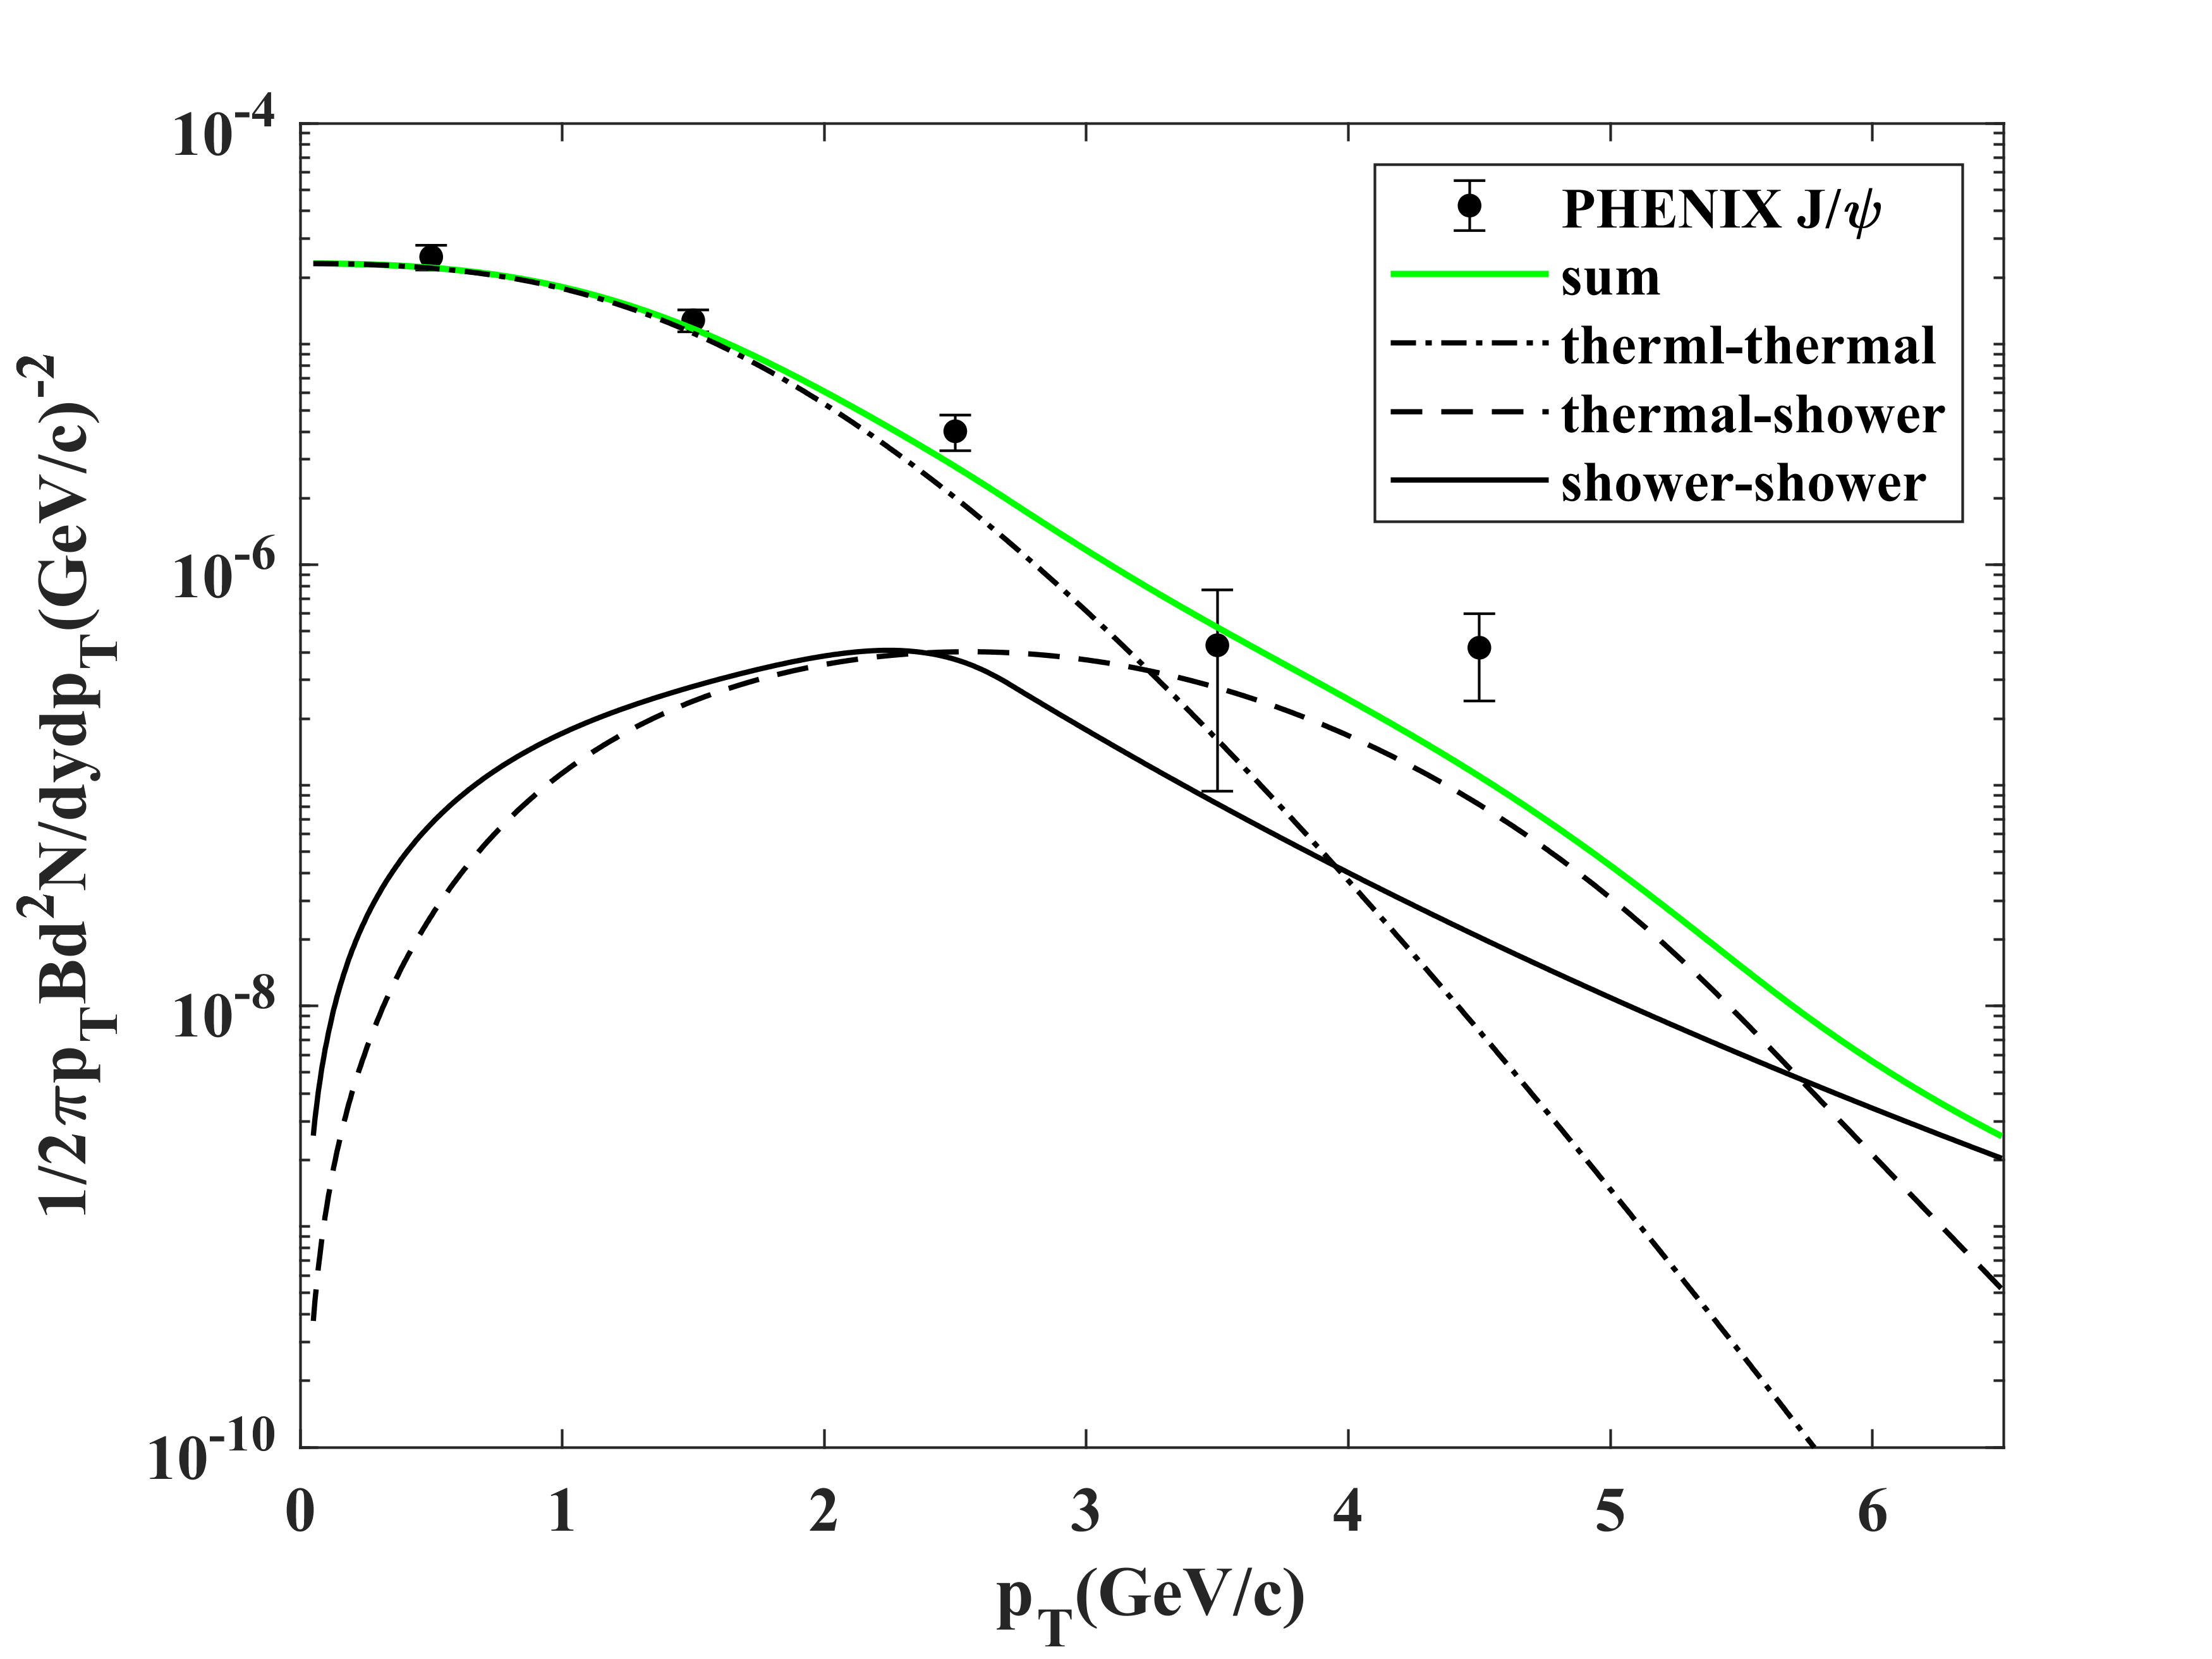
\includegraphics[width=0.45\textwidth]{Jpsi_200GeV.png}
		\caption{Transverse momentum spectra of $J/\psi$ at 200 GeV.}
		\label{fig1}
	\end{figure}
	\begin{figure}[pht]
	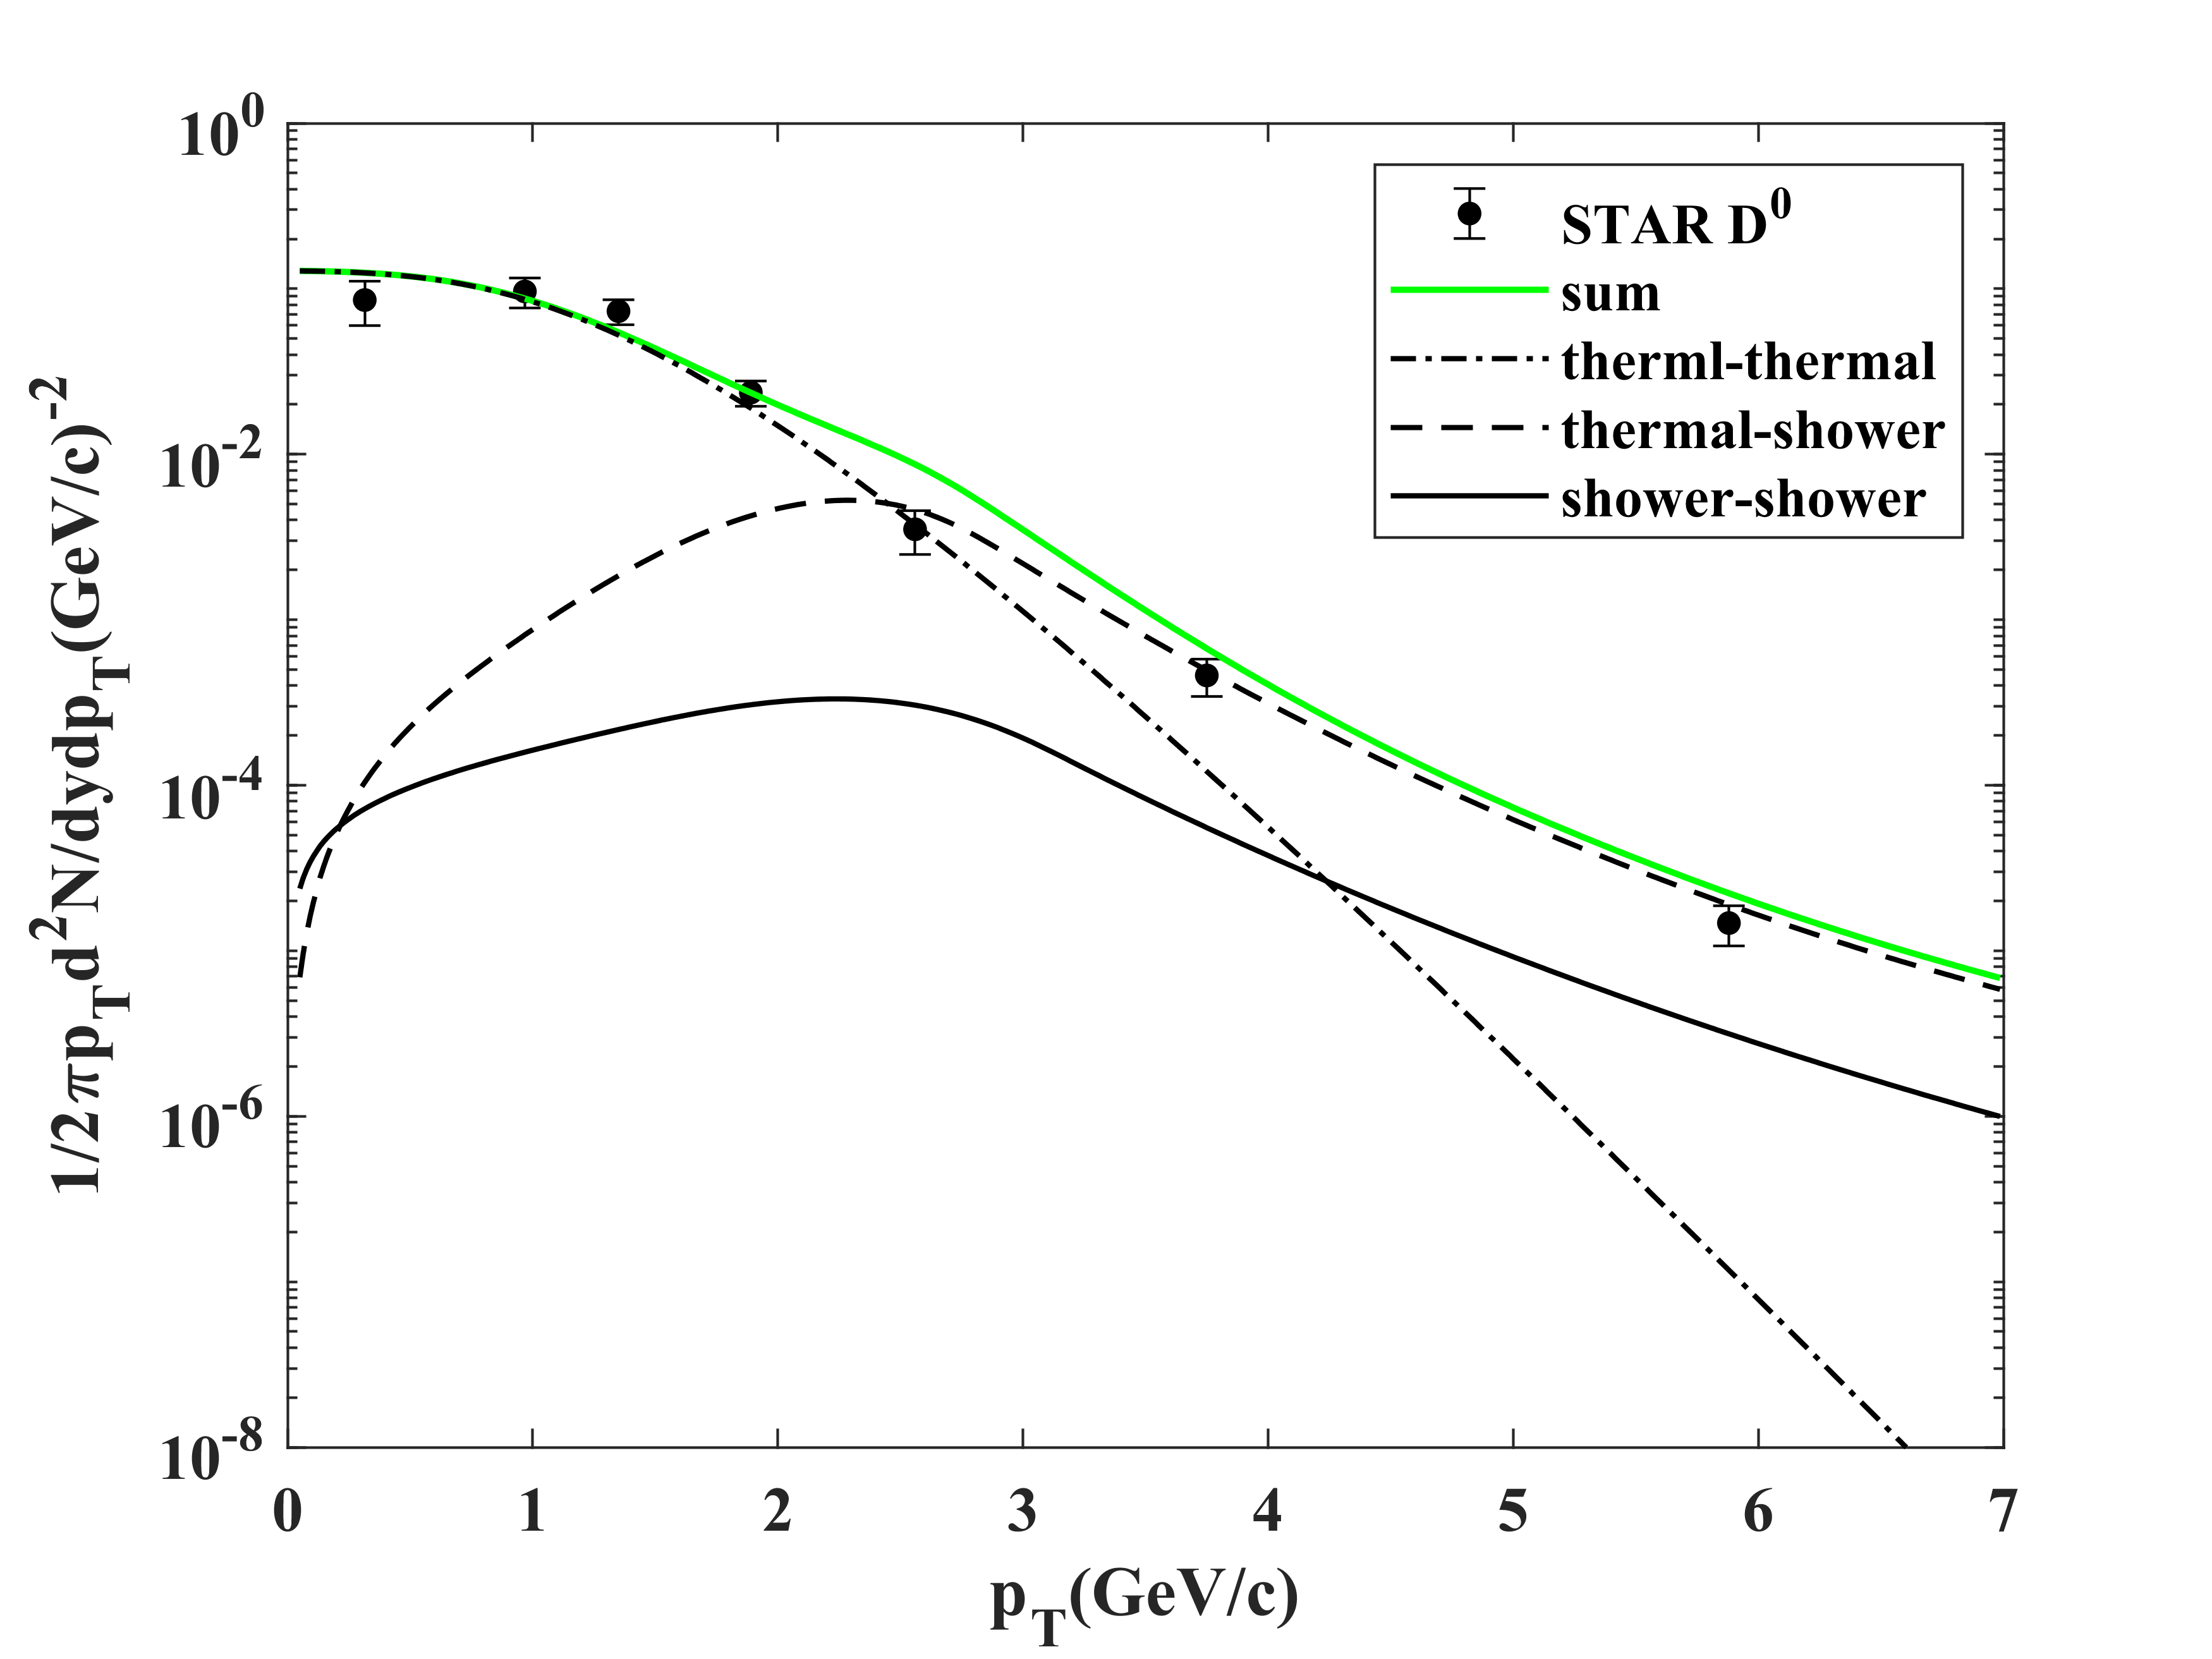
\includegraphics[width=0.45\textwidth]{D0_200GeV.png}
	\caption{Transverse momentum spectra of $D^0$ at 200 GeV.}
	\label{fig2}
	\end{figure}
	\begin{figure}[pht]
	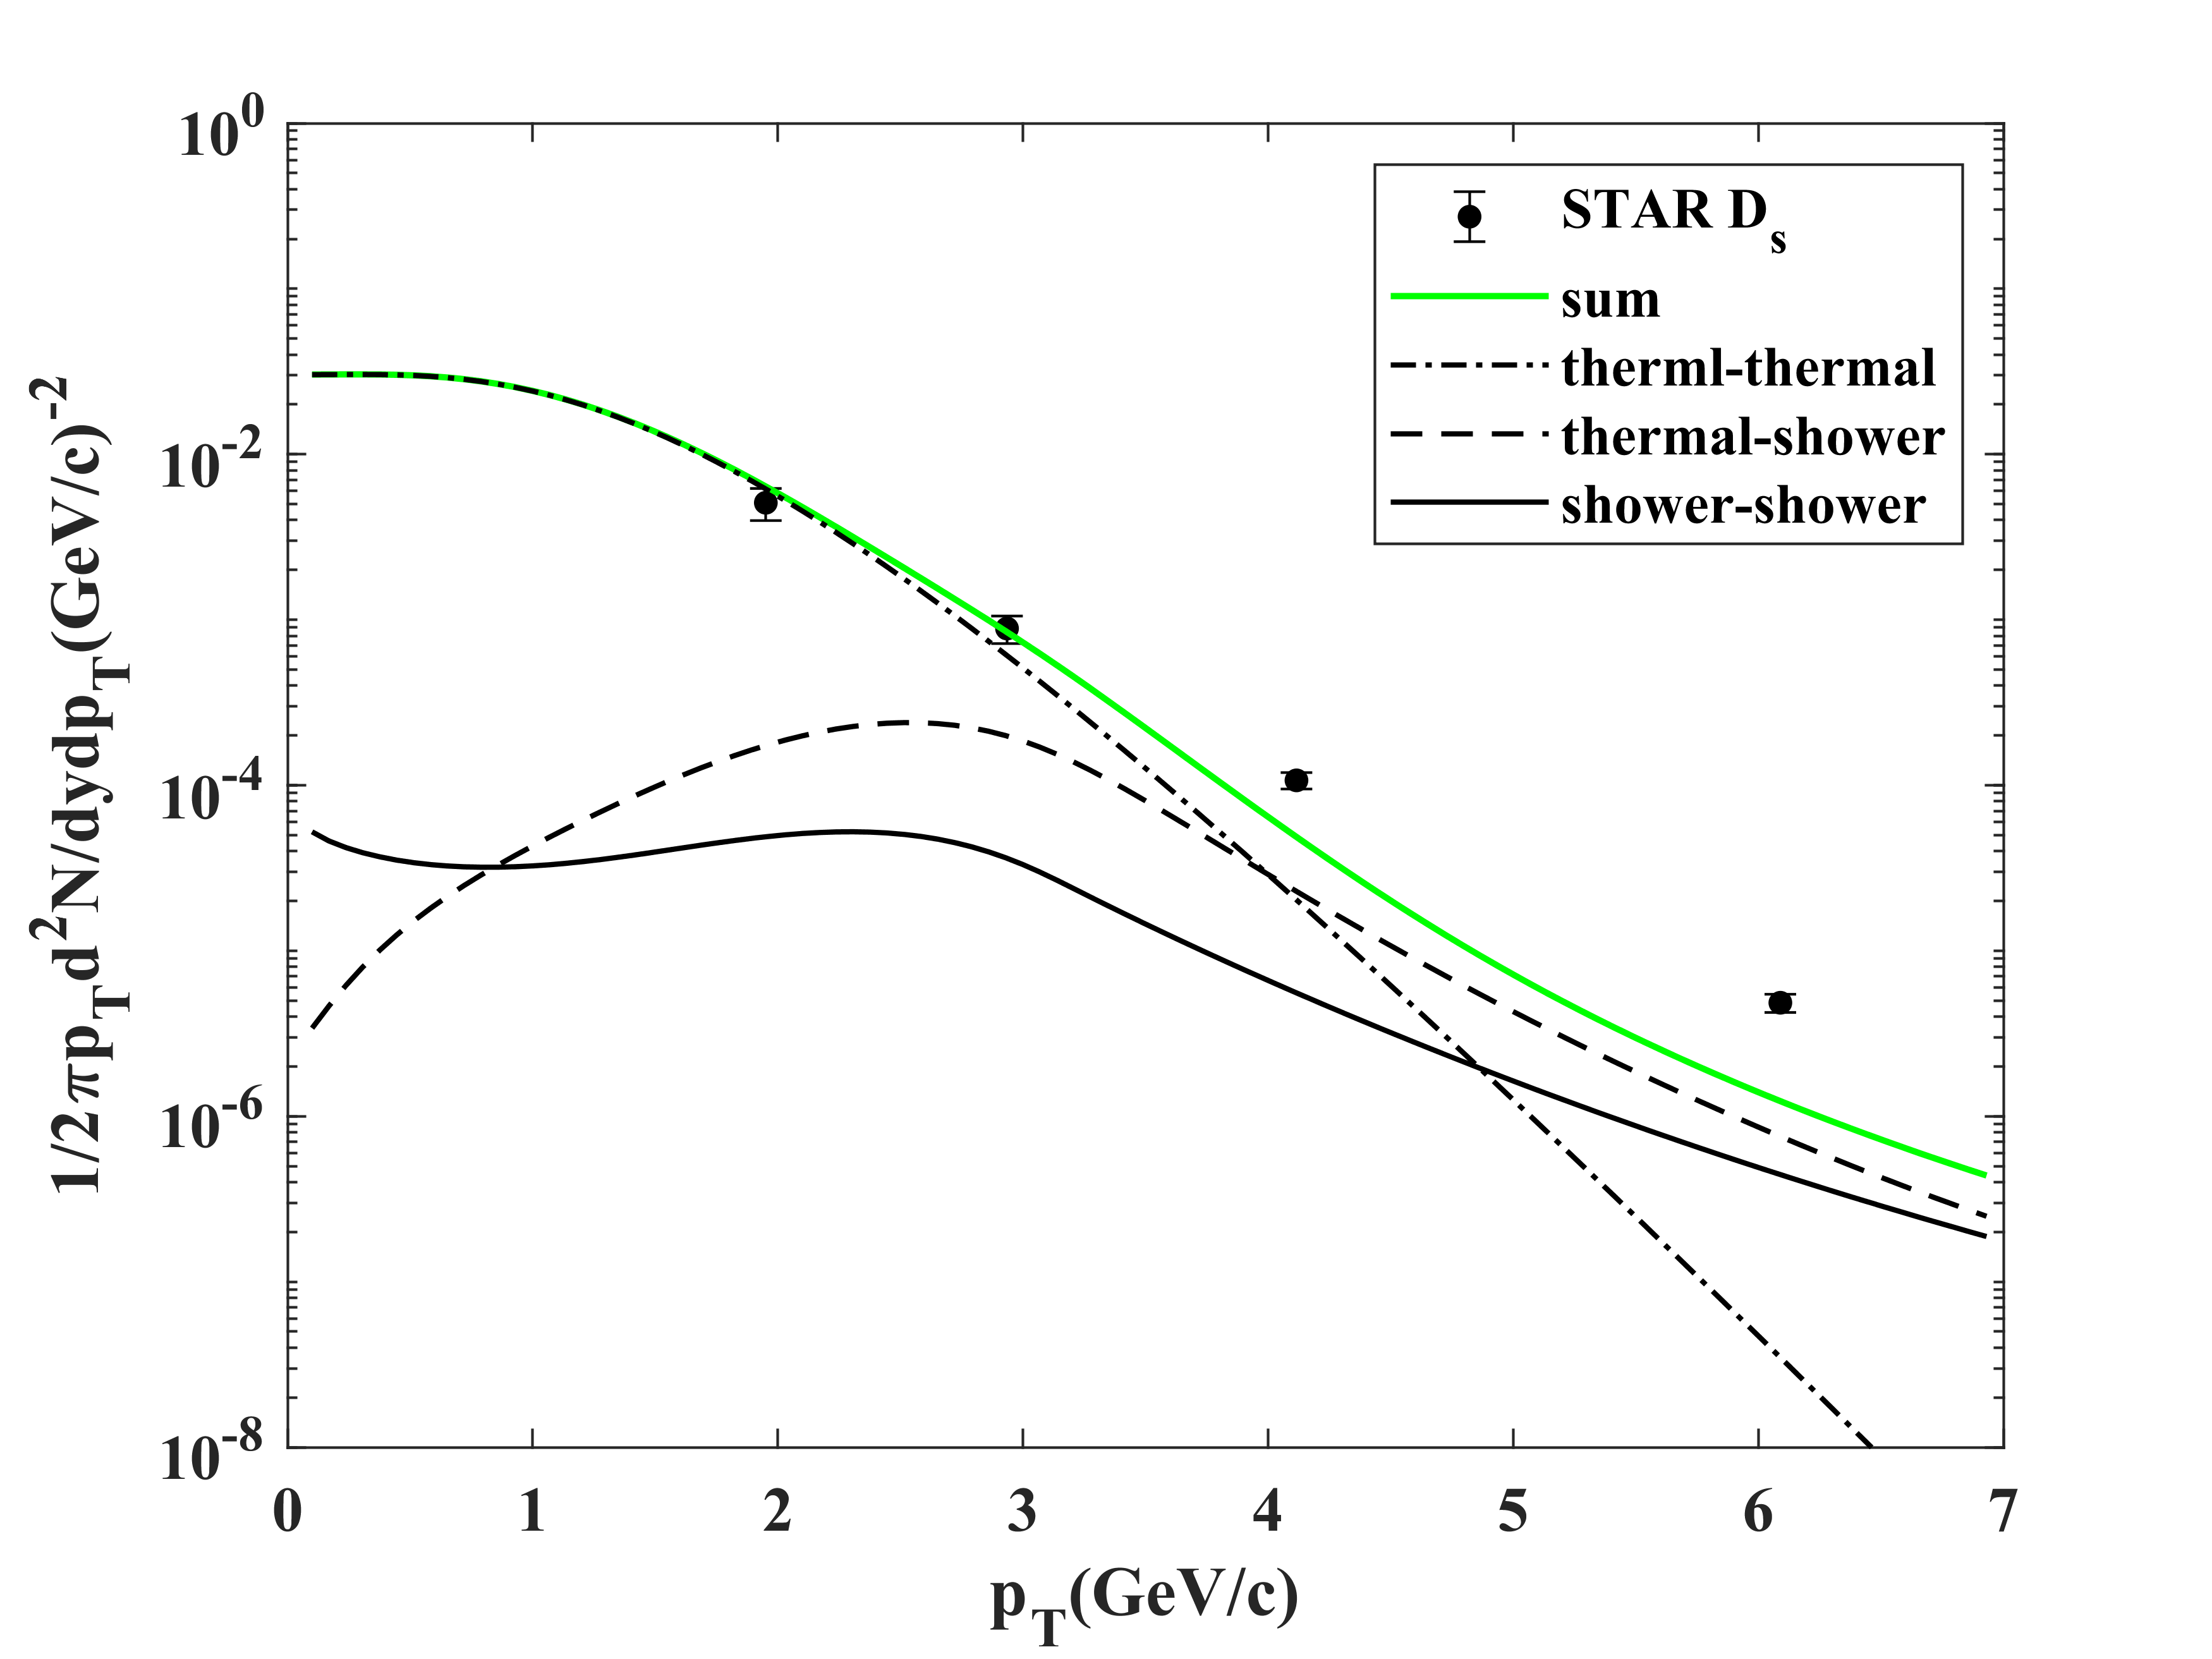
\includegraphics[width=0.45\textwidth]{Ds_200GeV.png}
	\centering
	\caption{Transverse momentum spectra of $D_s$ at 200 GeV.}
	\label{fig3}
	\end{figure}
	
	
\section{urgent questions}
	Data for $J/\psi, D^0, D_s$ at $\sqrt{s_{NN}}$=2.76/5.02 TeV are found in the form of $dN/dp_T$ \cite{jpsi_276, jpsi_502, D0_276,D0_502,Ds_276,Ds_502}, which need to be multiplied by $1/2\pi p_T$. Change of energy only leads to the various coefficients in $f_i(k)$, which has impact on $TT$ and $TS$ terms. Moreover, some parameters, e.g. $\gamma, v_T, \beta L, ect$, may need to be reoptimized.
	
	As for $f_i(k)$, parameters for the initial hard parton distribution at $\sqrt{s_{NN}}$=200 GeV (RHIC) and 5.5 TeV (LHC) are available in \cite{fik14, fik15}, which are not certainly reliable at $\sqrt{s_{NN}}$=2.76/5.02 TeV.
	\bq
		f_i(p_T)=\frac{dN^{jet}}{d^2p_T dy}=K\frac{C}{(1+p_T/B)^\beta}\label{fik}
	\eq
	 For $u, \bar u, d, \bar d, g, s, \bar s$ quark, we can obtain parameters at 2.76 and 5.02 TeV  by logarithmic interpolations between 200 GeV and 5.5 TeV for $lnA, B, \beta$ \cite{Zhu_2020}, whereas parameters for $c/\bar c$ are still not known. Following the notion in \cite{Zhu_2020}, we get the parameters in Eq.\ref{fik} at 2.76 and 5.02 TeV.
	
	The initial $p_T$ spectra of charm quarks at midrapidity at 200 GeV is taken to be
	\bq
		f_c(p_T)=\frac{dN_c}{d^2 p_T}=
		\frac{19.2\left[1+(p_T/6)^2\right]}{(1+p_T/3.7)^{12}\left[1+\text{exp}(0.9-2p_T)\right] }
	\eq
	which is obtained by multiplying the heavy quark $p_T$ spectra from p+p collisions at same energy by the number of binary collisions (\textasciitilde 960) in Au+Au collisions \cite{fik15}.
	
	For LHC energies (5.5 TeV) we take the initial $p_T$ spectra of charm quark at midrapidity from the perturbative calculation multiplied by the number of binary collisions ( \textasciitilde 1700) \cite{Liu:2008bw}.
	\begin{eqnarray}
	f_c(p_T)&=&\frac{dN_c}{d^2 p_T}\nonumber\\ 
	&=&2497(1+\frac{p_T}{1.95})^{-5.5}
	\left(p_T\left[1+\left(\frac{4}{0.1+p_T }\right)^2\right] \right)^{-1}	
	\end{eqnarray}
	Thus, we now just use the formula at 5.5 TeV for 2.76/5.02 TeV, as it is rough to generalize them to 2.76/5.02 TeV. 
	
	Besides, while it is negligible at $\sqrt{s_{NN}}$=200 GeV, the new component of the two-jet contribution $SS(2)$ should be taken into account at $\sqrt{s_{NN}}$=2.76/5.02 TeV, which is given by \cite{Peng:2011zzd}
	\begin{eqnarray}
		\frac{dN^{SS(2)}}{pdp}&=&\frac{1}{p^0p}\sum_{i,i'} \int \frac{dq}{q}\frac{dq'}{q'}F_i(q)F_{i'}(q')\Gamma(q,q')   \\ 
		&\times& \int\frac{dp_1}{p_1}\frac{dp_2}{p_2}F_{ii'}(q,q';p_1,p_2)R_M(p_1,p_2,p).\nonumber
	\end{eqnarray}
	 More details are shown in the next section. Then, the first results are shown in Figs.\ref{fig4}, \ref{fig5}, \ref{fig6}.
	
	\begin{figure}[H]
		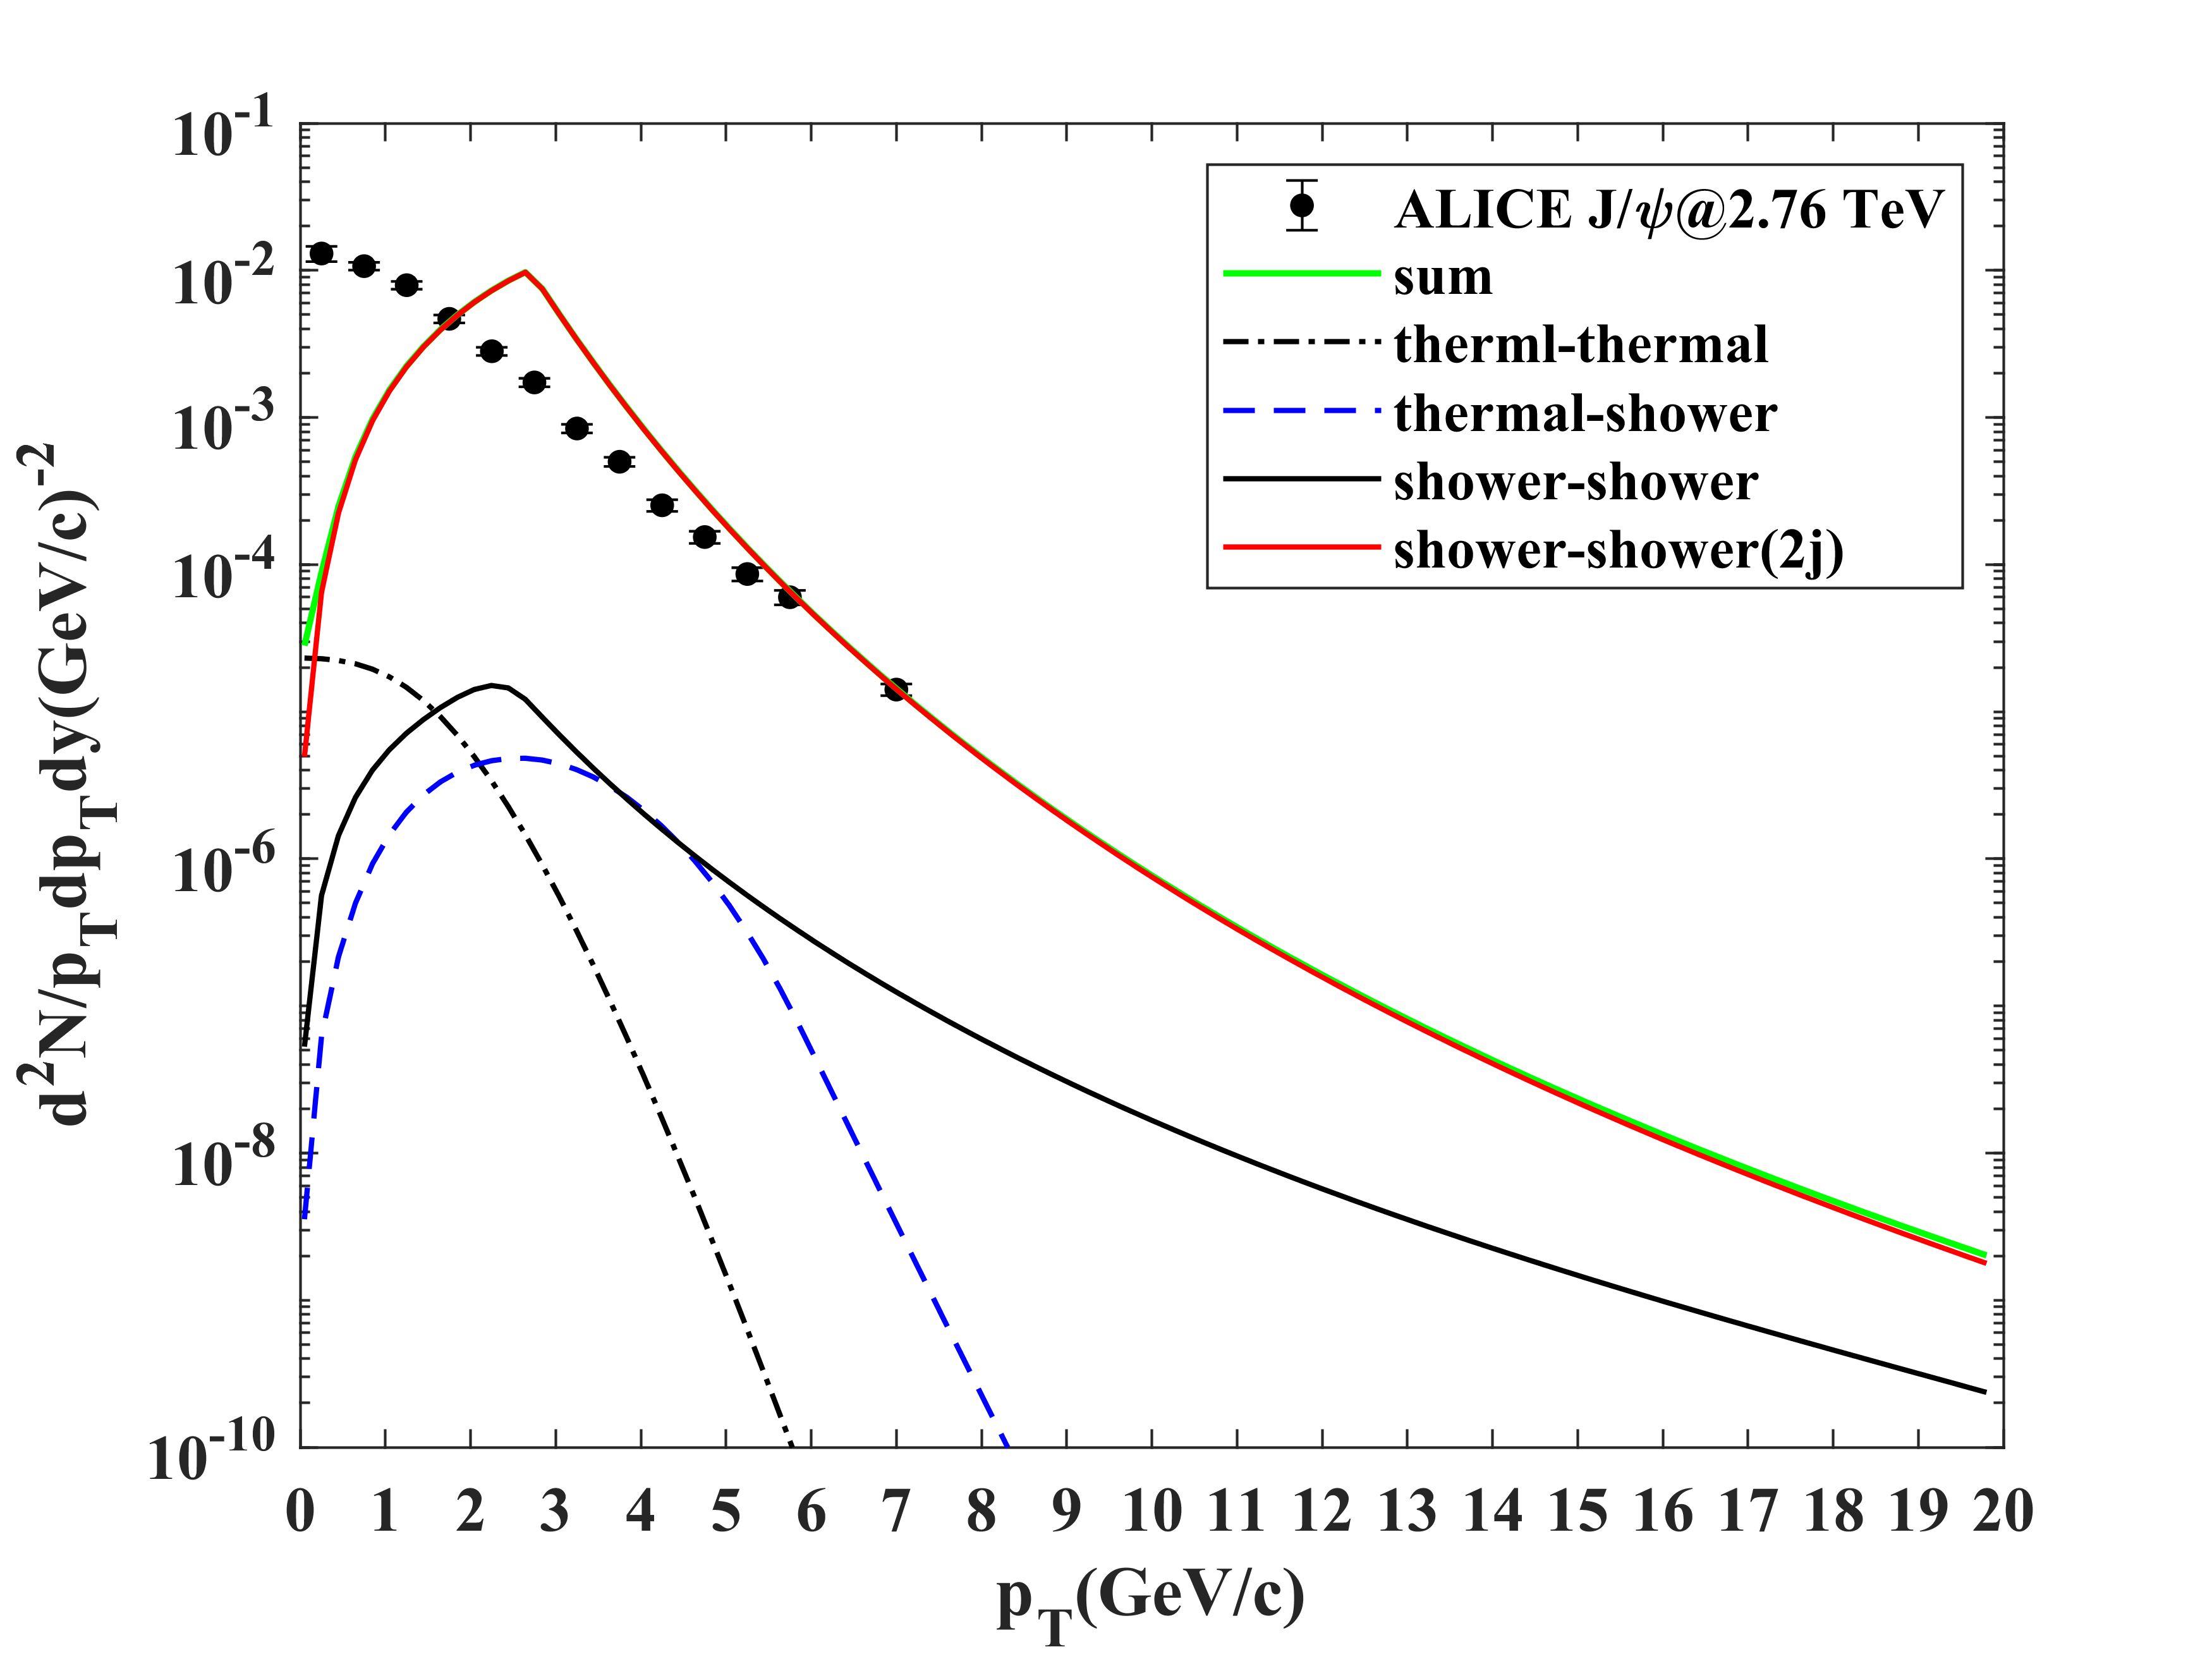
\includegraphics[width=0.45\textwidth]{Jpsi_276_1st.png}
		\caption{Transverse momentum spectra of $J/\psi$ at 2.76 TeV with $\Gamma=10^{-3}$.}
		\label{fig4}
	\end{figure}
	\begin{figure}[H]
		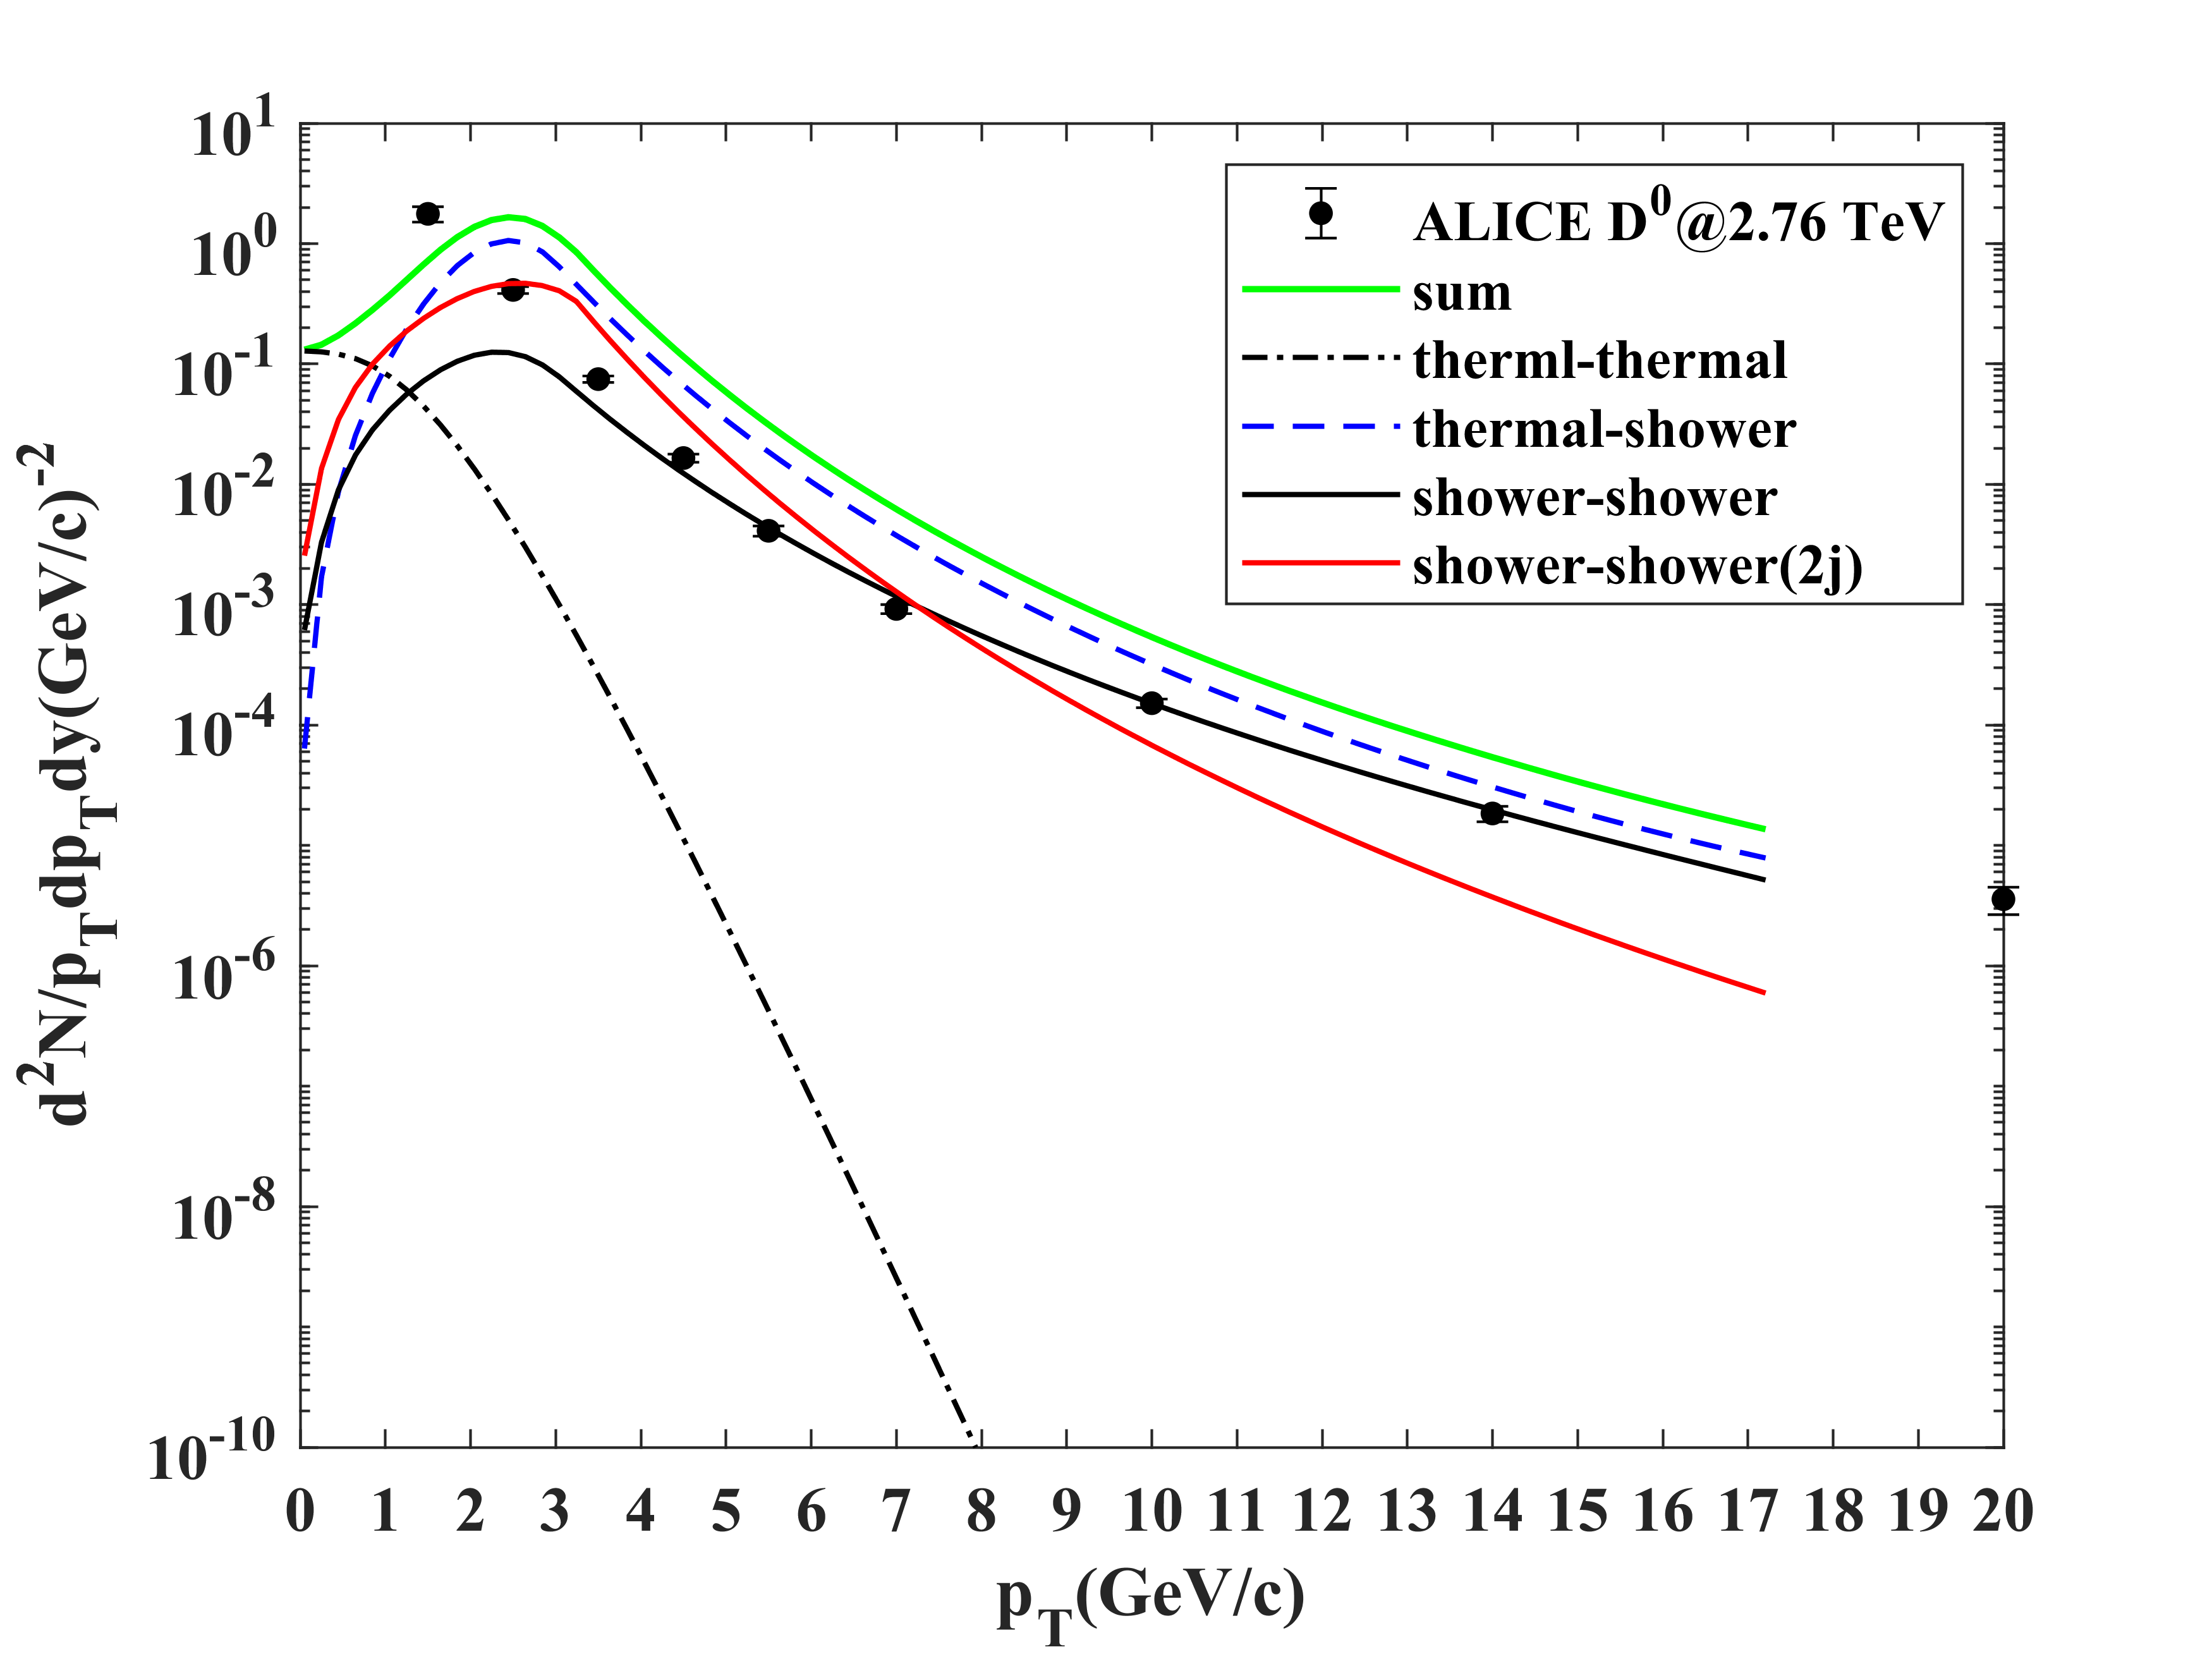
\includegraphics[width=0.45\textwidth]{D0_276_1st.png}
		\caption{Transverse momentum spectra of $D^0$ at 2.76 TeV with $\Gamma=10^{-3}$.}
		\label{fig5}
	\end{figure}
	\begin{figure}[H]
		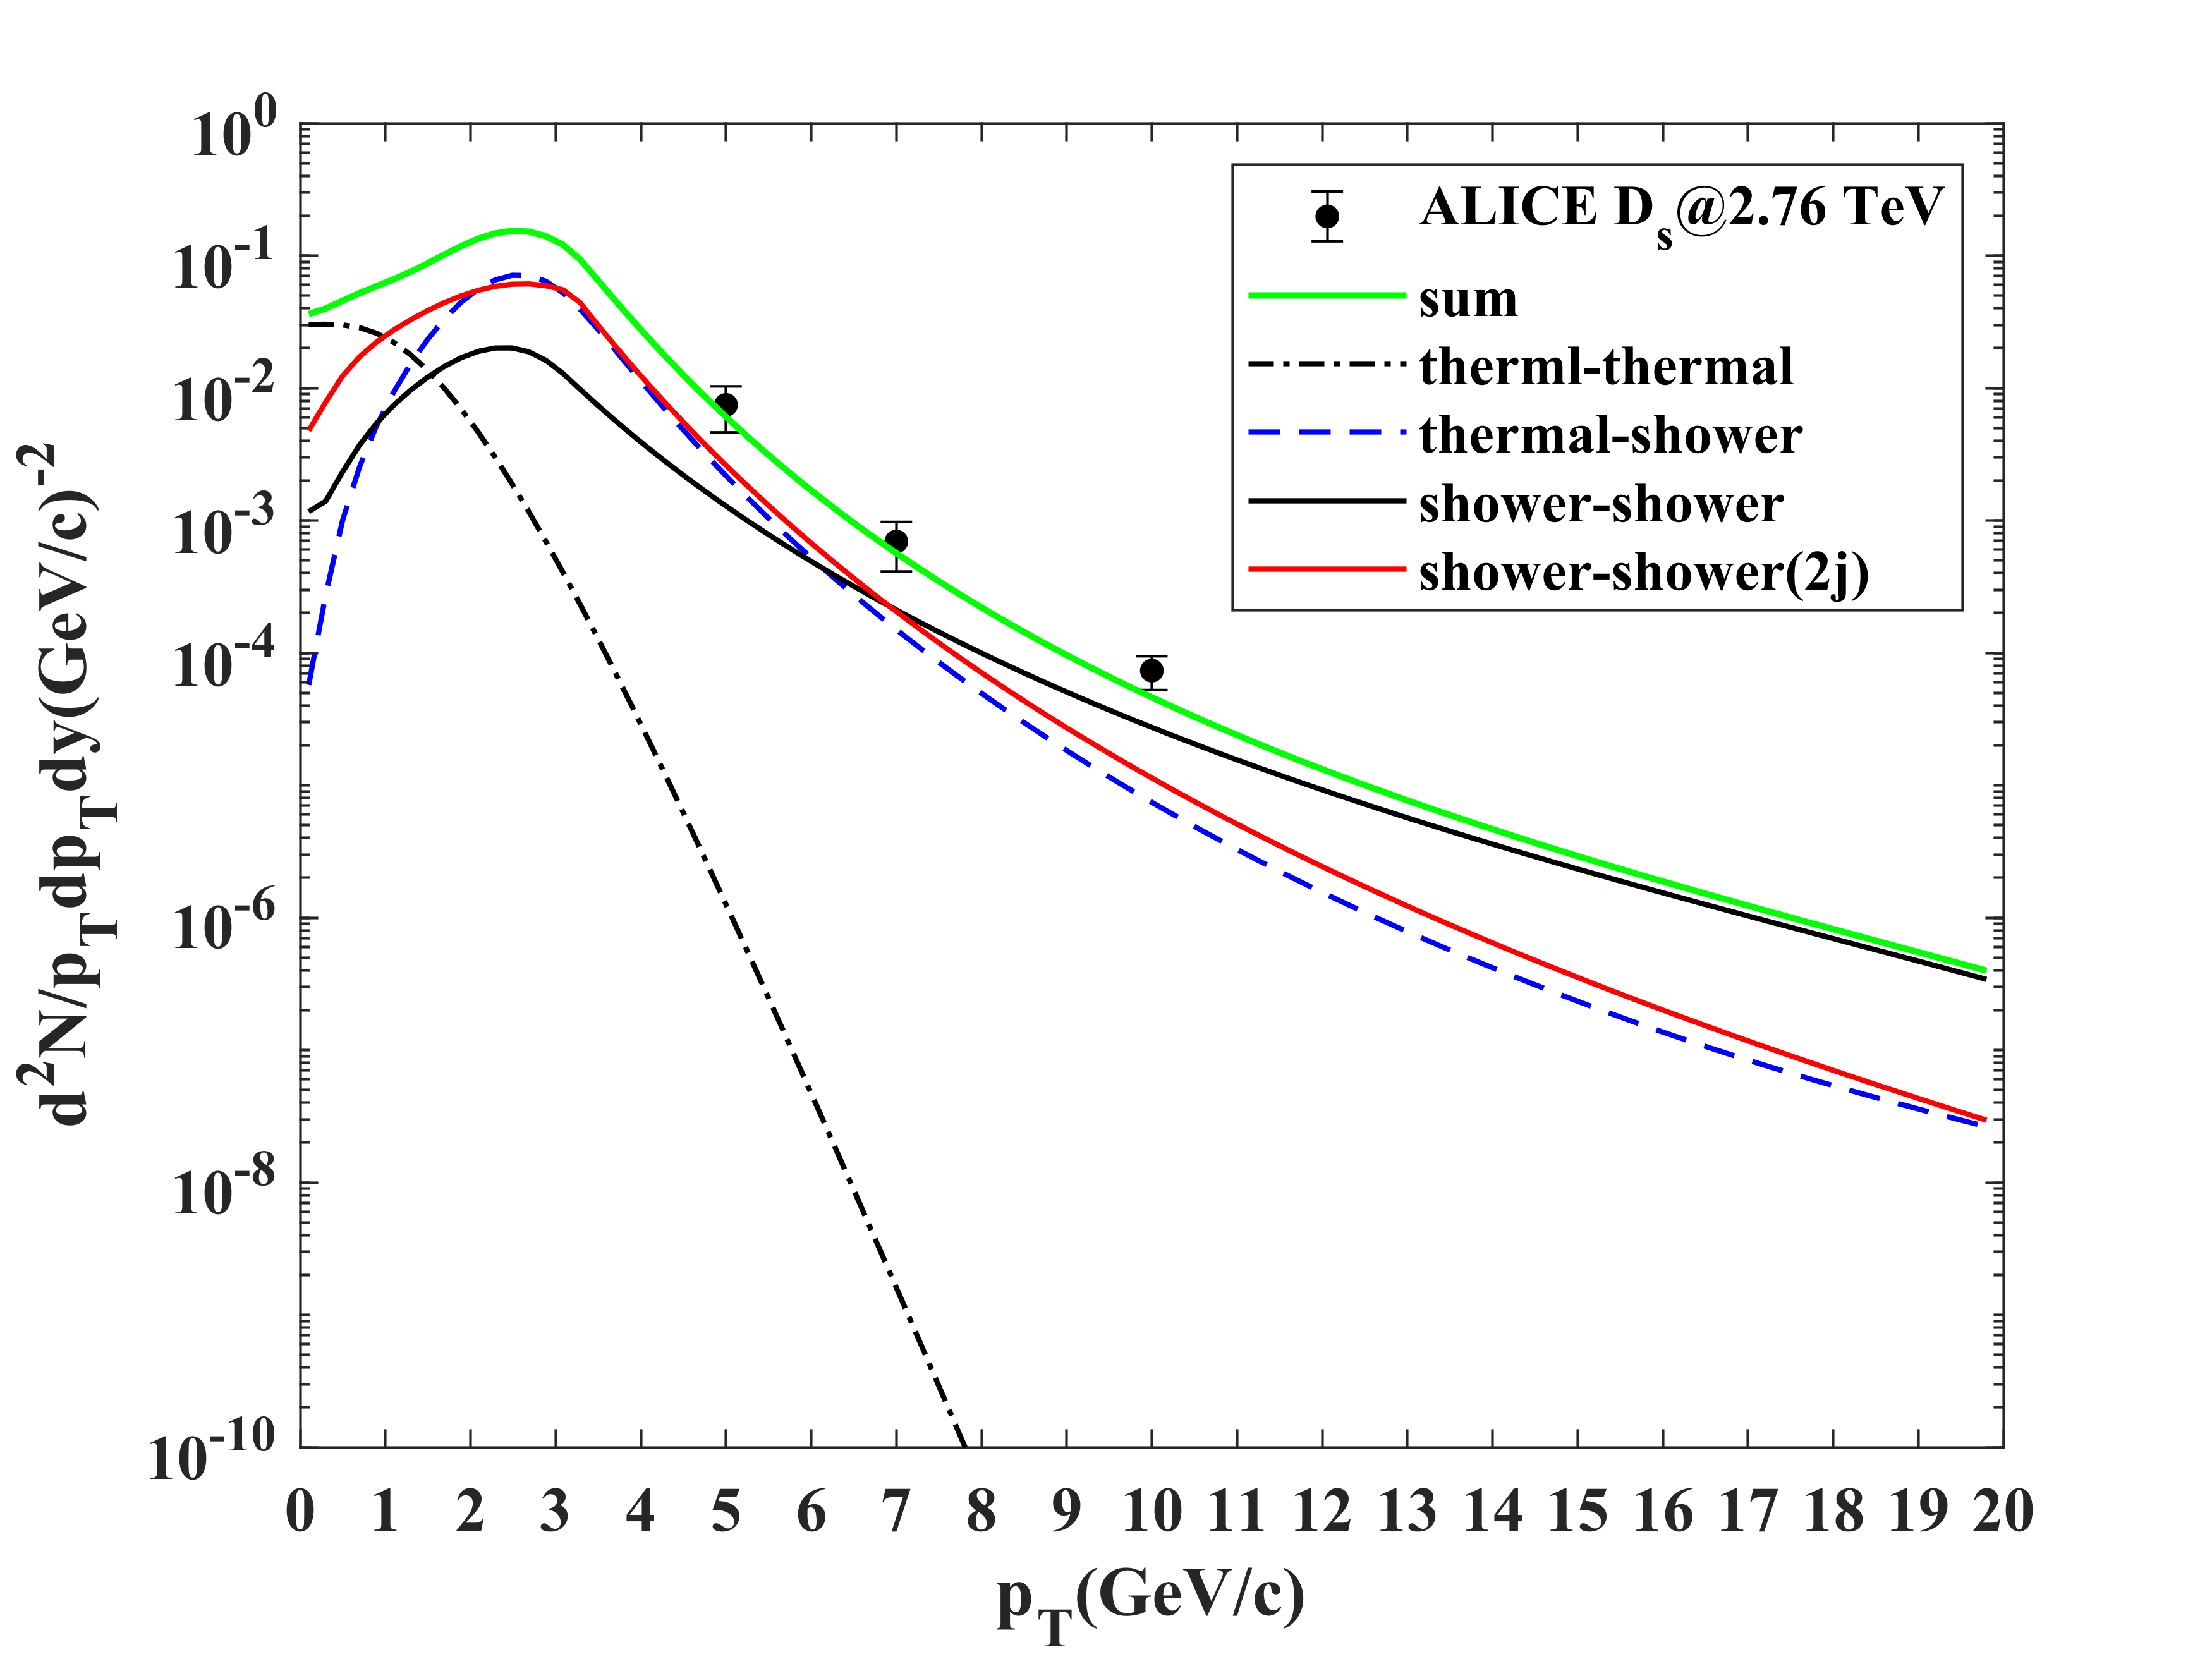
\includegraphics[width=0.45\textwidth]{Ds_276_1st.png}
		\caption{Transverse momentum spectra of $D_s$ at 2.76 TeV with $\Gamma=10^{-3}$.}
		\label{fig6}
	\end{figure}
	
\section{fit and optimization}
Since last meeting, two ideas are put forward. First, the contribution $TT$ should be optimized by fitting $\eta_T$. Second, $f_i(k)$ in Pb+Pb at 2.76 and 5.02 TeV should be given, which cannot be replaced by that at 5.5 TeV.

As a result, we find that the change of $v_T$ can effect only one order of magnitude of $TT$. But the running mass of charm does matter in $T$ composition. The change $m_c$ from 1.5 to 1.2 can fit the data at least in $TT$, although $v_T=0.1c$ and $\gamma_c=1.1$ can also fit the data. Consequently, we fix $\gamma_c=0.26$, $v_T=0.25c$, temperature $T=0.185$ GeV and $m_c=1.28$, fitted by thermal parton distribution at low $p_T$.

 Here, we give the four contributions again as follows. And notice that the results of $TS$, $SS(1j)$,  $SS(2j)$ terms are multiplied by a factor of $1-e^{-p/2}$ to suppress the low $p$ contribution.
 
\subsection{$TT$ term} 
\begin{eqnarray}
	\frac{dN^{TT}_{M}}{d^2p}&=&C_M M_T \frac{\tau A_T}{(2\pi)^3}2\gamma_a\gamma_b I_0\left[\frac{psinh\eta_T}{T}\right]  \nonumber\\
	&&\times \int_{0}^{1}dx \vert \phi_M(x)\vert^2 k_M(x,p),
\end{eqnarray}
where 
\begin{eqnarray}
	k_M(x,p)=K_1\left[\frac{cosh\eta_T}{T}(\sqrt{m_a^2+p_1^2}+\sqrt{m_b^2+p_2^2})\right]
\end{eqnarray}
\begin{eqnarray}
	\vert \phi_M(x)\vert^2={1\over B(a,b)}x^{a-1}(1-x)^{b-1}
\end{eqnarray}
and $p_1=xp, p_2=(1-x)p, A_T=\rho_0^2\pi$ with the radius $\rho_0=9$ fm, the meson degeneracy factor $C_M=(2\times3)^2$. It was assumed that hadronization occurs at $\tau$ = 5 fm with temperature $T$ = 0.175 GeV in the parton phase. $I_0$ and $K_1$ are the modified Bessel functions. Moreover, the fugacities of light quarks are $\gamma_u=\gamma_d=1$ and for the strange quarks $\gamma_s=0.8$. The free parameters are fugacity $\gamma_c=0.26$(fixed) and transverse flow rapidity $\eta_T$ defined by a flow velocity with $v_T=tanh \eta_T$. Fitted by experimental data in Au+Au collision at RHIC energy, we have obtained $v_T=0.3c(J/\psi)$ and  $v_T=0.42c(D^0)$.


\subsection{$TS$ term}
\begin{eqnarray}
	\frac{dN^{TS}_{M}}{d^2p}=C_M\int_{0}^{1}&&dx \vert \phi_M(x)\vert^2 \\ 
	&\times &\left[{T_a(p_1)S_b(p_2)\over g\gamma_a x}+{S_a(p_1)T_b(p_2)\over g\gamma_b (1-x)}\right] \nonumber
\end{eqnarray}
with $g$ = 6 coming from the color and spin degeneracy of a quark. And the thermal parton spectrum
\begin{eqnarray}
	T_a(p)={2g\gamma_a m_T \over (2\pi)^3}I_0\left[\frac{psinh\eta_T}{T}\right]K_1\left[\frac{m_T cosh\eta_T}{T}\right].
\end{eqnarray}
Then, the  the distribution of shower parton $j$
\begin{eqnarray}
	S_j(p)=\sum_i \int {dq\over q}F_i(q)S_i^j(p/q),
\end{eqnarray}
where
\begin{eqnarray}
	F_i(q)={1\over \beta L}\int_{q}^{q e^{\beta L}} {dk\over k}f'_i(k),
\end{eqnarray}
with $f'_i(k)=f_i(k) (2\pi)^3/E$.

\subsection{$SS(1j)$ term}
\begin{eqnarray}
	\frac{dN^{SS(1)}_{M}}{pdp}={1\over p^0p}\sum_i \int {dq\over q}F'_i(q)
	{p\over q}D_i^M({p\over q}),	
\end{eqnarray}
where
\begin{eqnarray}
	F'_i(q)={1\over \beta L}\int_{q}^{q e^{\beta L}} dkk f_i(k),
\end{eqnarray}
and $D_i^M$ is the FF of quark i splitting into meson M.
\begin{eqnarray}
	xD_i^H(x)=\int_0^x {dx_1 \over x_1}\int_0^x {dx_2 \over x_2} \{S_i^q(x_1),S_i^{\overline{q'}} (x_2)\}R(x_1,x_2,x).
\end{eqnarray}

\subsection{$SS(2j)$ term}
Besides, while it is negligible at $\sqrt{s_{NN}}$=200 GeV, the new component of the two-jet contribution $SS(2)$ should be taken into account at $\sqrt{s_{NN}}$=2.76/5.02 TeV, which is given by \cite{Peng:2011zzd}
\begin{eqnarray}
	\frac{dN^{SS(2)}}{pdp}&=&\frac{1}{p^0p}\sum_{i,i'} \int \frac{dq}{q}\frac{dq'}{q'}F'_i(q)F'_{i'}(q')\Gamma(q,q')   \\ 
	&\times& \int\frac{dp_1}{p_1}\frac{dp_2}{p_2}F_{ii'}(q,q';p_1,p_2)R_M(p_1,p_2,p).\nonumber
\end{eqnarray}
In the above expression, $F_{ii′}$ is the distribution of shower partons related to the two jets
and for a meson it is written as
\begin{eqnarray}
	F_{ii'}(q,q';p_1,p_2)=S_i^j({p_1\over q})S_{i'}^{j'}({p_2\over q'}),
\end{eqnarray}
and since we have not sufficient information of such dependencies for collisions at
LHC, the overlap function is approximated by an average quantity $\Gamma$ which varies over a wide range  $\Gamma=10^{-n}$ with $n=1,2,3$ and 4.

Specifically, we simply the formulae of 3 mesons respectively for numerical computing as follows:
\begin{eqnarray}
	\frac{dN^{SS(2)}_{J/\psi}}{pdp}&=&\frac{10^{-n}}{p^0p}\sum_{\substack{i=g,c\\ i'=g,c}} \int \frac{dq}{q}\frac{dq'}{q'}F'_i(q)F'_{i'}(q')\nonumber \\
	&&\times  S_i^{\overline c}({p\over 2q})   S_{i'}^c({p\over 2q'}), \label{ss2_jpsi}
\end{eqnarray}
\begin{eqnarray}
	\frac{dN^{SS(2)}_{D^0}}{pdp}&=&\frac{5*10^{-n}}{p^0p^6}\sum_{\substack{i=q,\overline q,g\\ i'=g,c}} \int \frac{dq}{q}\frac{dq'}{q'}F'_i(q)F'_{i'}(q')\nonumber \\
	&&\times \int_0^q dp_2 S_i^{\overline u}({p-p_2\over q})   S_{i'}^c({p_2\over q'})p_2^4,
\end{eqnarray}
\begin{eqnarray}
	\frac{dN^{SS(2)}_{D_s}}{pdp}&=&\frac{660*10^{-n}}{p^0p^{13}}\sum_{\substack{i=q,\overline q,g,s,\overline s\\ i'=g,c}} \int \frac{dq}{q}\frac{dq'}{q'}F'_i(q)F'_{i'}(q')\nonumber \\
	&&\times \int_0^q dp_2 S_i^{\overline s}({p-p_2\over q})   S_{i'}^c({p_2\over q'})
	p_2^9(p-p_2)^2,
\end{eqnarray}

To testify the accuracy of calculations, we reproduce the results (transverse momentum spectra for $J/\psi$ at 5.5 TeV) in Ref.\cite{Peng:2011zzd}, shown in Fig.\ref{fig11}, which has a good agreement with the reference.
\begin{figure}[H]
	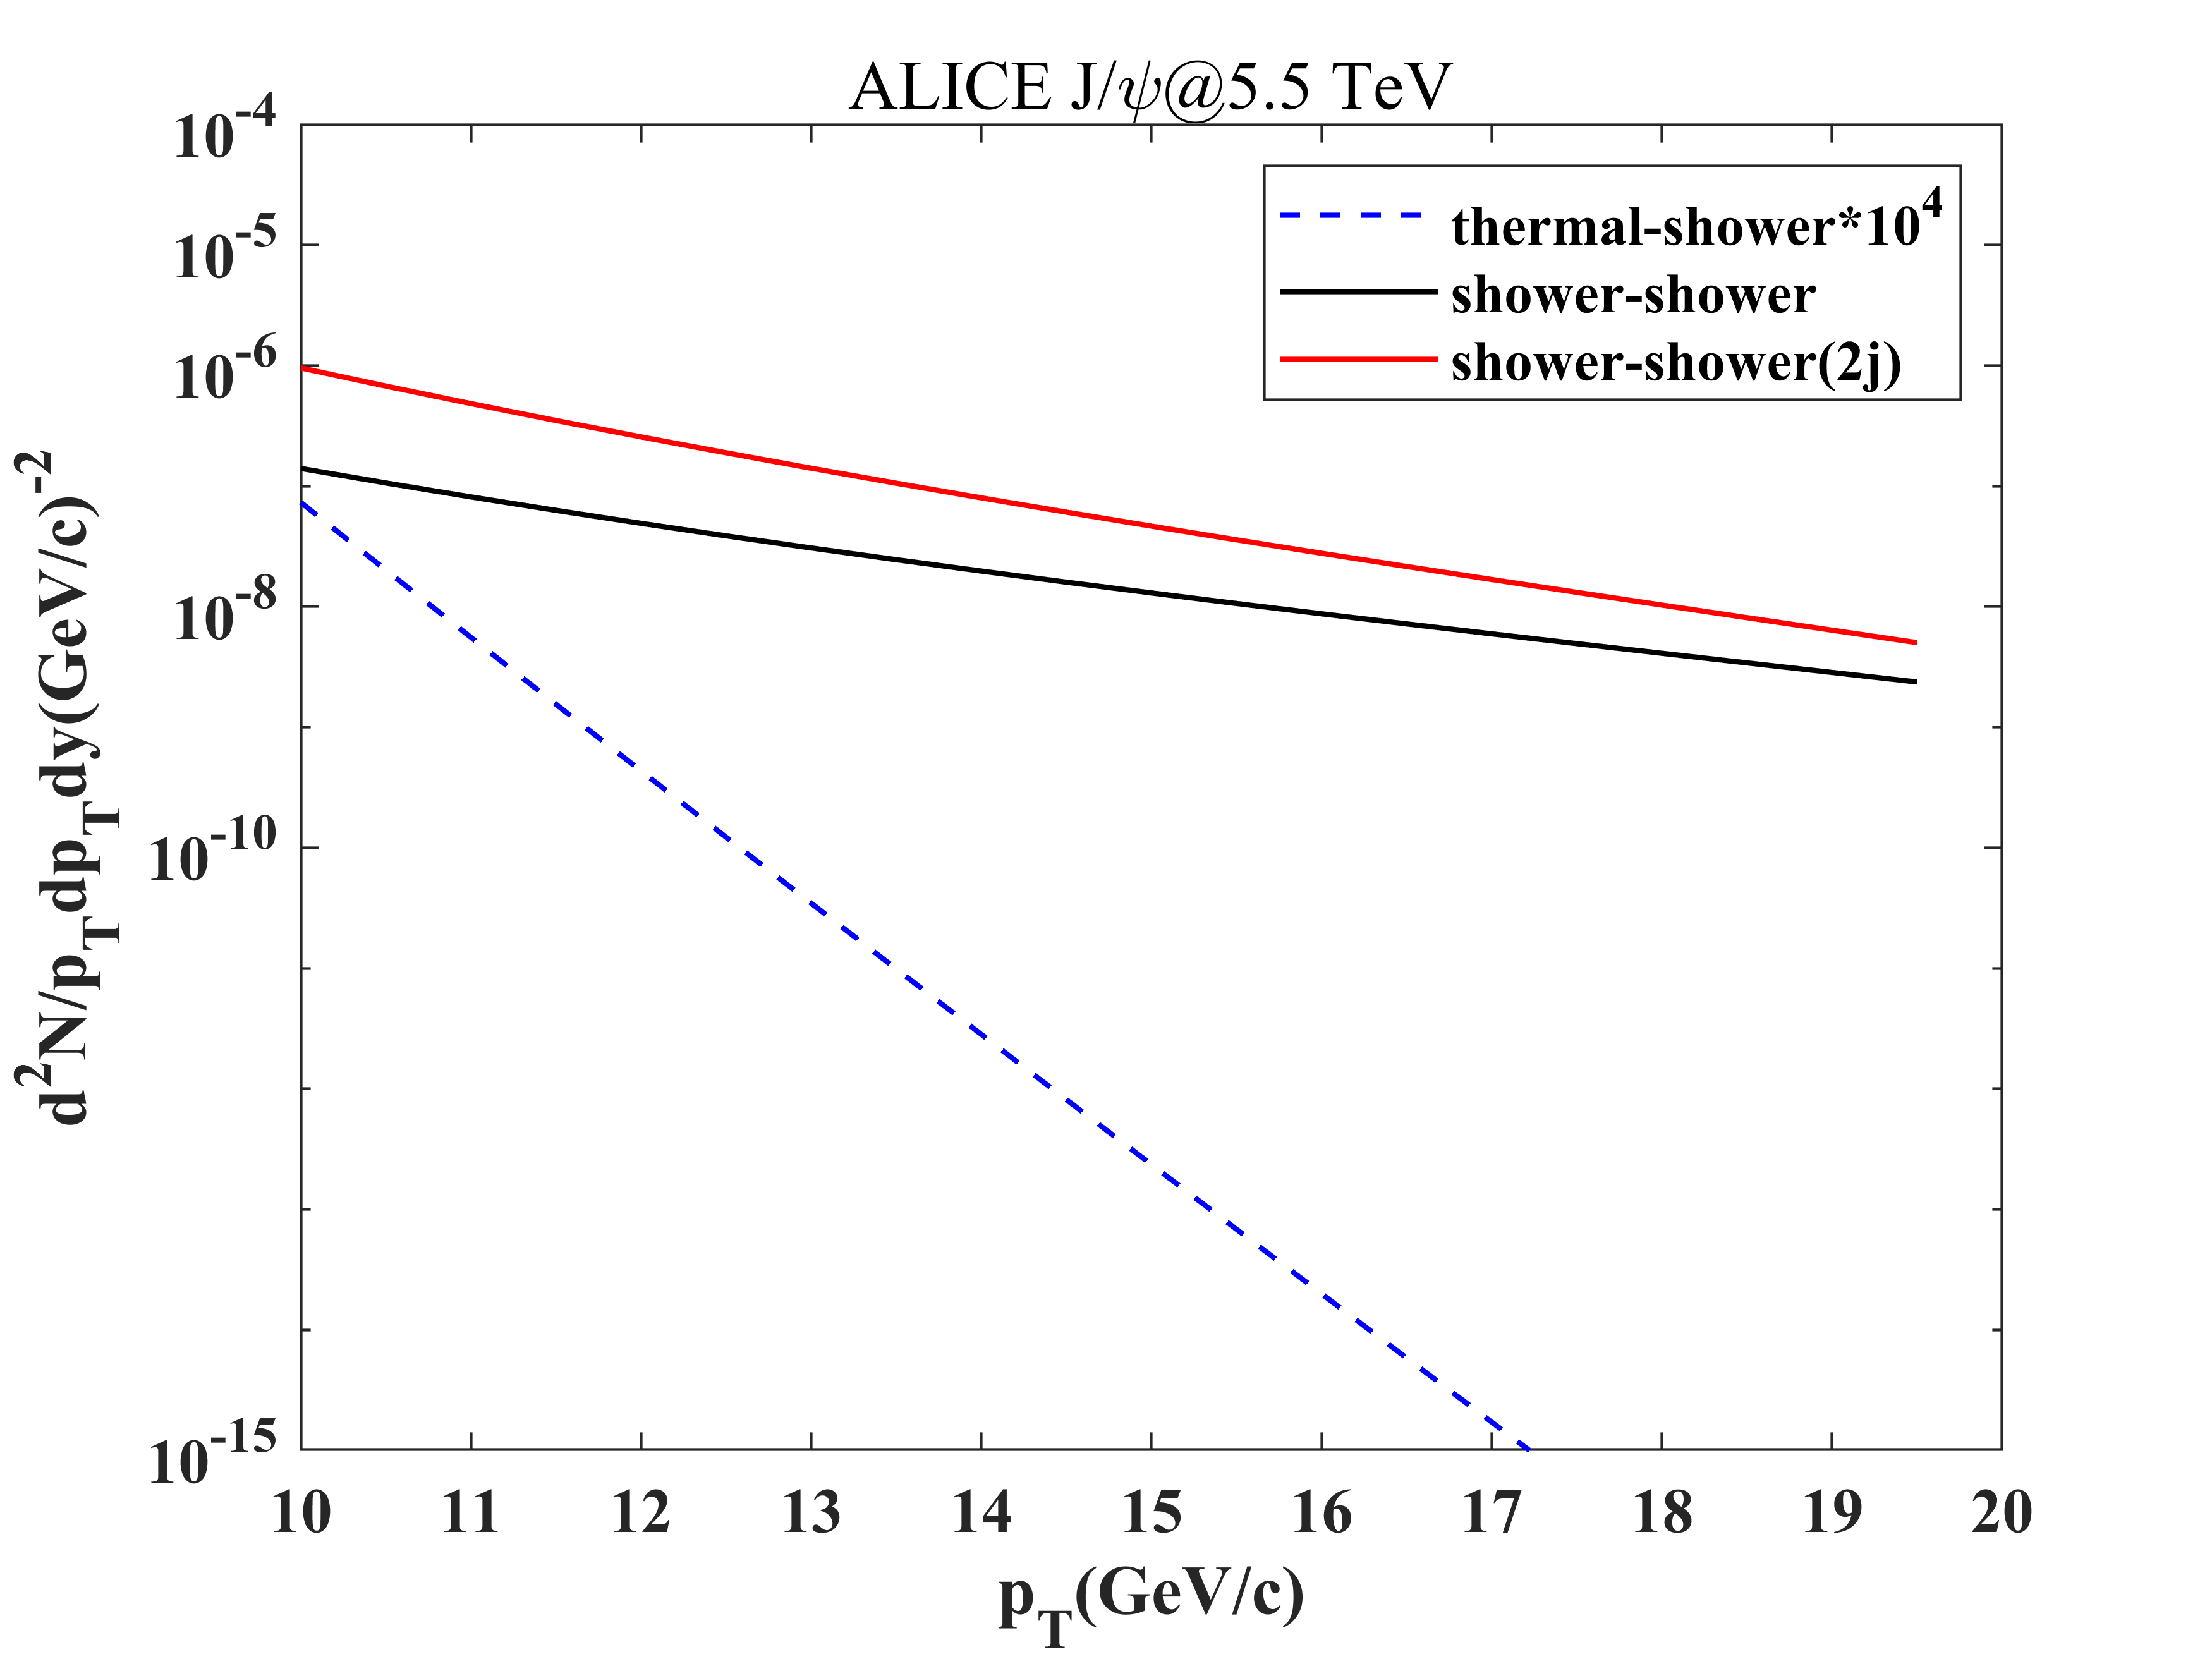
\includegraphics[width=0.45\textwidth]{repro ref.png}
	\caption{The comparison of three terms for $J/\psi$ at 5.5 TeV with $\Gamma=10^{-2}$.}
	\label{fig11}
\end{figure}


\section{solution of hard parton distributions for charm}
After search and contacting some professors, it seems no one had studied parameterized initial charm quark distribution. Thus, we attempt to figure out interpolated functions at 2.76/5.5 TeV between 200 GeV and 5.5 TeV to solve it.

Because of known formula of u quark, we compare the parameterized results at various energy, shown in Fig. \ref{fig7}. Obviously, $\ln(f_i(k))$ is not linear with $\sqrt{s_{NN}}$, otherwise the curve of 2.76 TeV should be almost at the position where two curves of 5.5 TeV and 0.2 TeV are bisected. For simplicity, it is assumed that $\ln(f_i^{\sqrt{s}}(k))$ is linear with $\ln(\sqrt{s_{NN}})$(in TeV), i.e. $f_i^{\sqrt{s}}(k)$ increases linearly with $\sqrt{s_{NN}}$. Therefore, hard parton distribution at any energy can be expressed:
\begin{eqnarray}
	\frac{f_i^{ \sqrt{s}}-f_i^{ 5.5}}{\sqrt{s}-5.5}=
	\frac{f_i^{ 0.2}-f_i^{ 5.5}}{0.2-5.5} \label{method_fik}
\end{eqnarray} 
Then, we give the deviation between our linear evaluation and parameterized values in Fig.\ref{fig8}, from which it is reasonable to accept the linear assumption. So we generalize this simple relation to initial charm quark distribution and get the distributions at 2.76 and 5.02 TeV successfully by linear combination of distributions at 0.2 and 5.5 TeV, shown in Fig.\ref{fig9}. We also give another results assuming $\ln(f_i(k))$ is linear with $\sqrt{s_{NN}}$ to trial, shown in Fig.\ref{fig10}.

Subsequently, we test the two $f_i(k)$, which is linear or exponential with $\sqrt{s_{NN}}$ respectively, by calculating the momentum spectra for $J/\psi$ at 2.76 TeV shown in Fig.\ref{fig12} and \ref{fig13}. Unfortunately, the former result, which should be logically compelling, is even worse than the latter, and both of all cannot fit the experiment data. But the latter conveys that the dominant components $SS(1j)$ and $SS(2j)$ in high transverse momentum determine the accuracy of fitting. And next step should be to determine further the shape of $f_i(k)$ for charm.

After that, from the high contribution of $SS$, it is reasonable to decrease $f_i(k)$ of charm. Therefore, we adjust the weight of $f_c(k)$ at 200 GeV from about 0.51, according to Eq.\ref{method_fik}, to 0.6 shown in Fig.\ref{improved fck}, improving the calculated $p_T$ distribution for $J/\psi, D^0, D_s$ at 2.76 TeV shown in Figs.\ref{fig14}, \ref{fig15}, \ref{fig16}. The parameters changed are list here:
\begin{eqnarray}
	J/\psi&:& v_T=0.25c, T=0.185 \text{ GeV}, \Gamma=5\times 10^{-3}, \\ \nonumber
						&&\beta L\rightarrow \text{0 for charm, 2.39 for gluon}\\
	D^0&:& v_T=0.43c, T=0.185 \text{ GeV}, \Gamma=10^{-2}, \\ \nonumber
						&&\beta L=\text{5.8 for all}\\
	D_s&:& v_T=0.3c, T=0.185\text{ GeV}, \Gamma=10^{-2}, \\ \nonumber
						&& \beta L=\text{5.0 for all}.
\end{eqnarray}

\begin{figure}[H]
	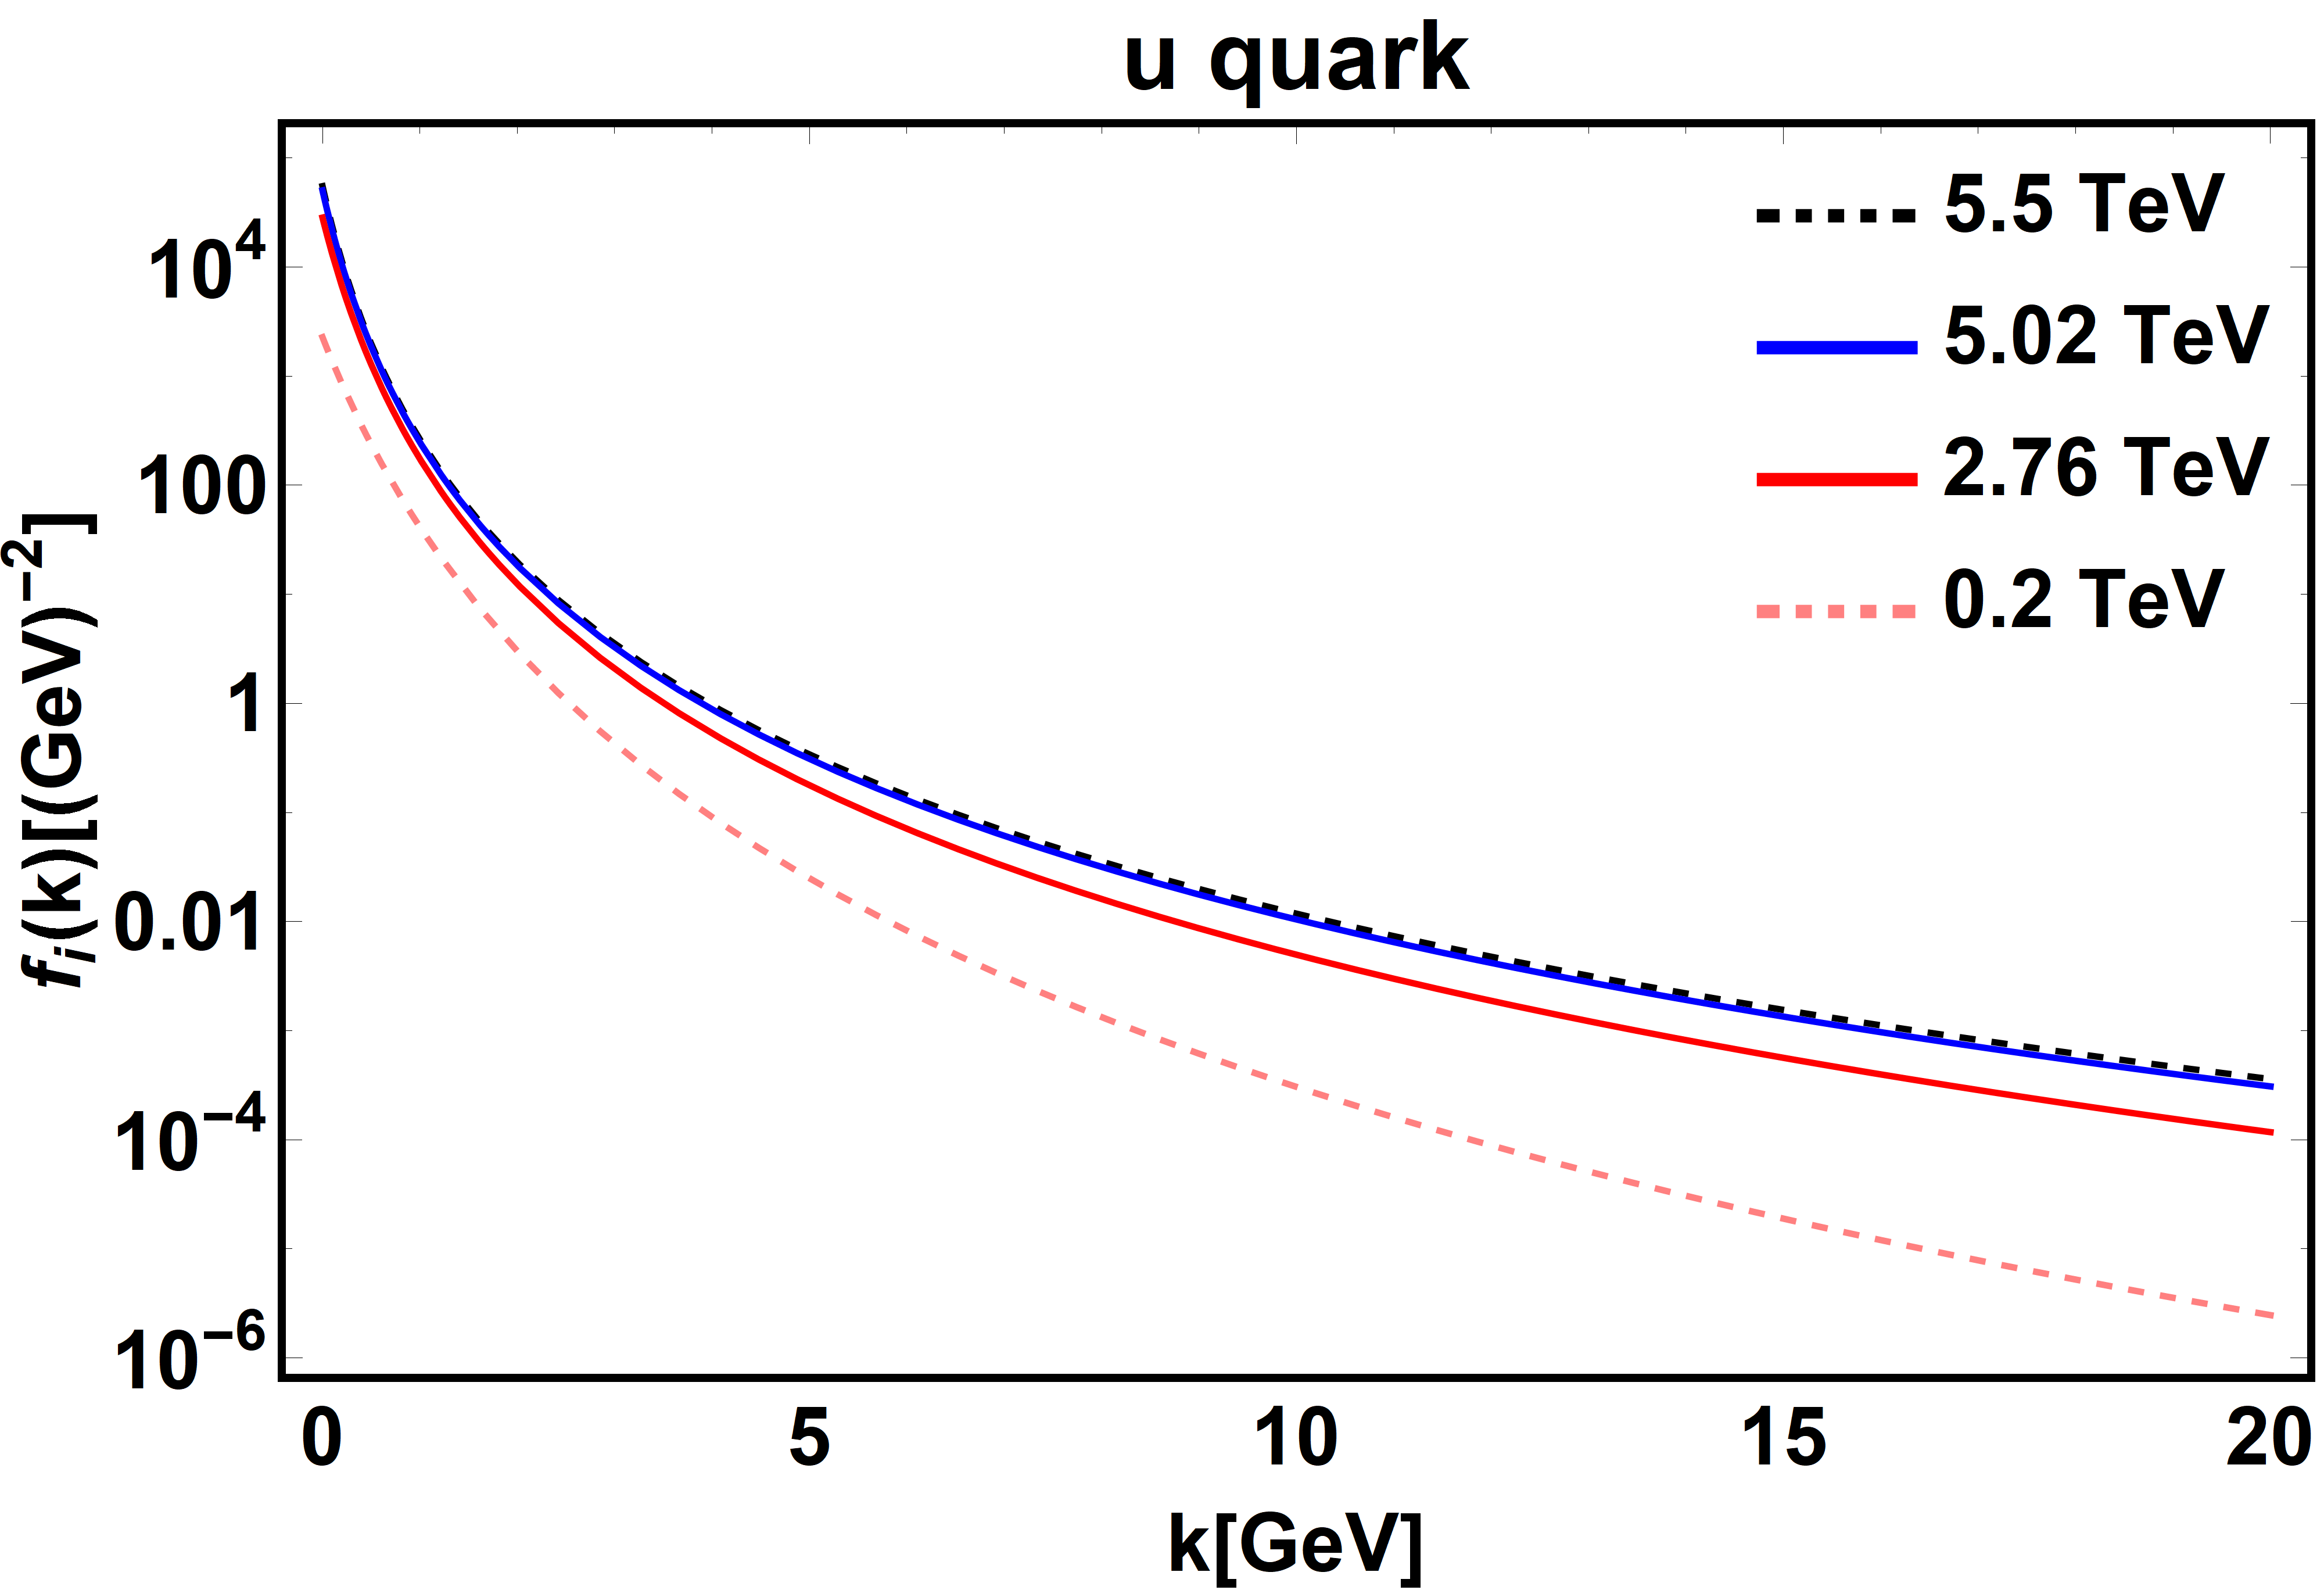
\includegraphics[width=0.45\textwidth]{fiku.png}
	\caption{Hard parton distribution of u quark at various energy.}
	\label{fig7}
\end{figure}

\begin{figure}[H]
	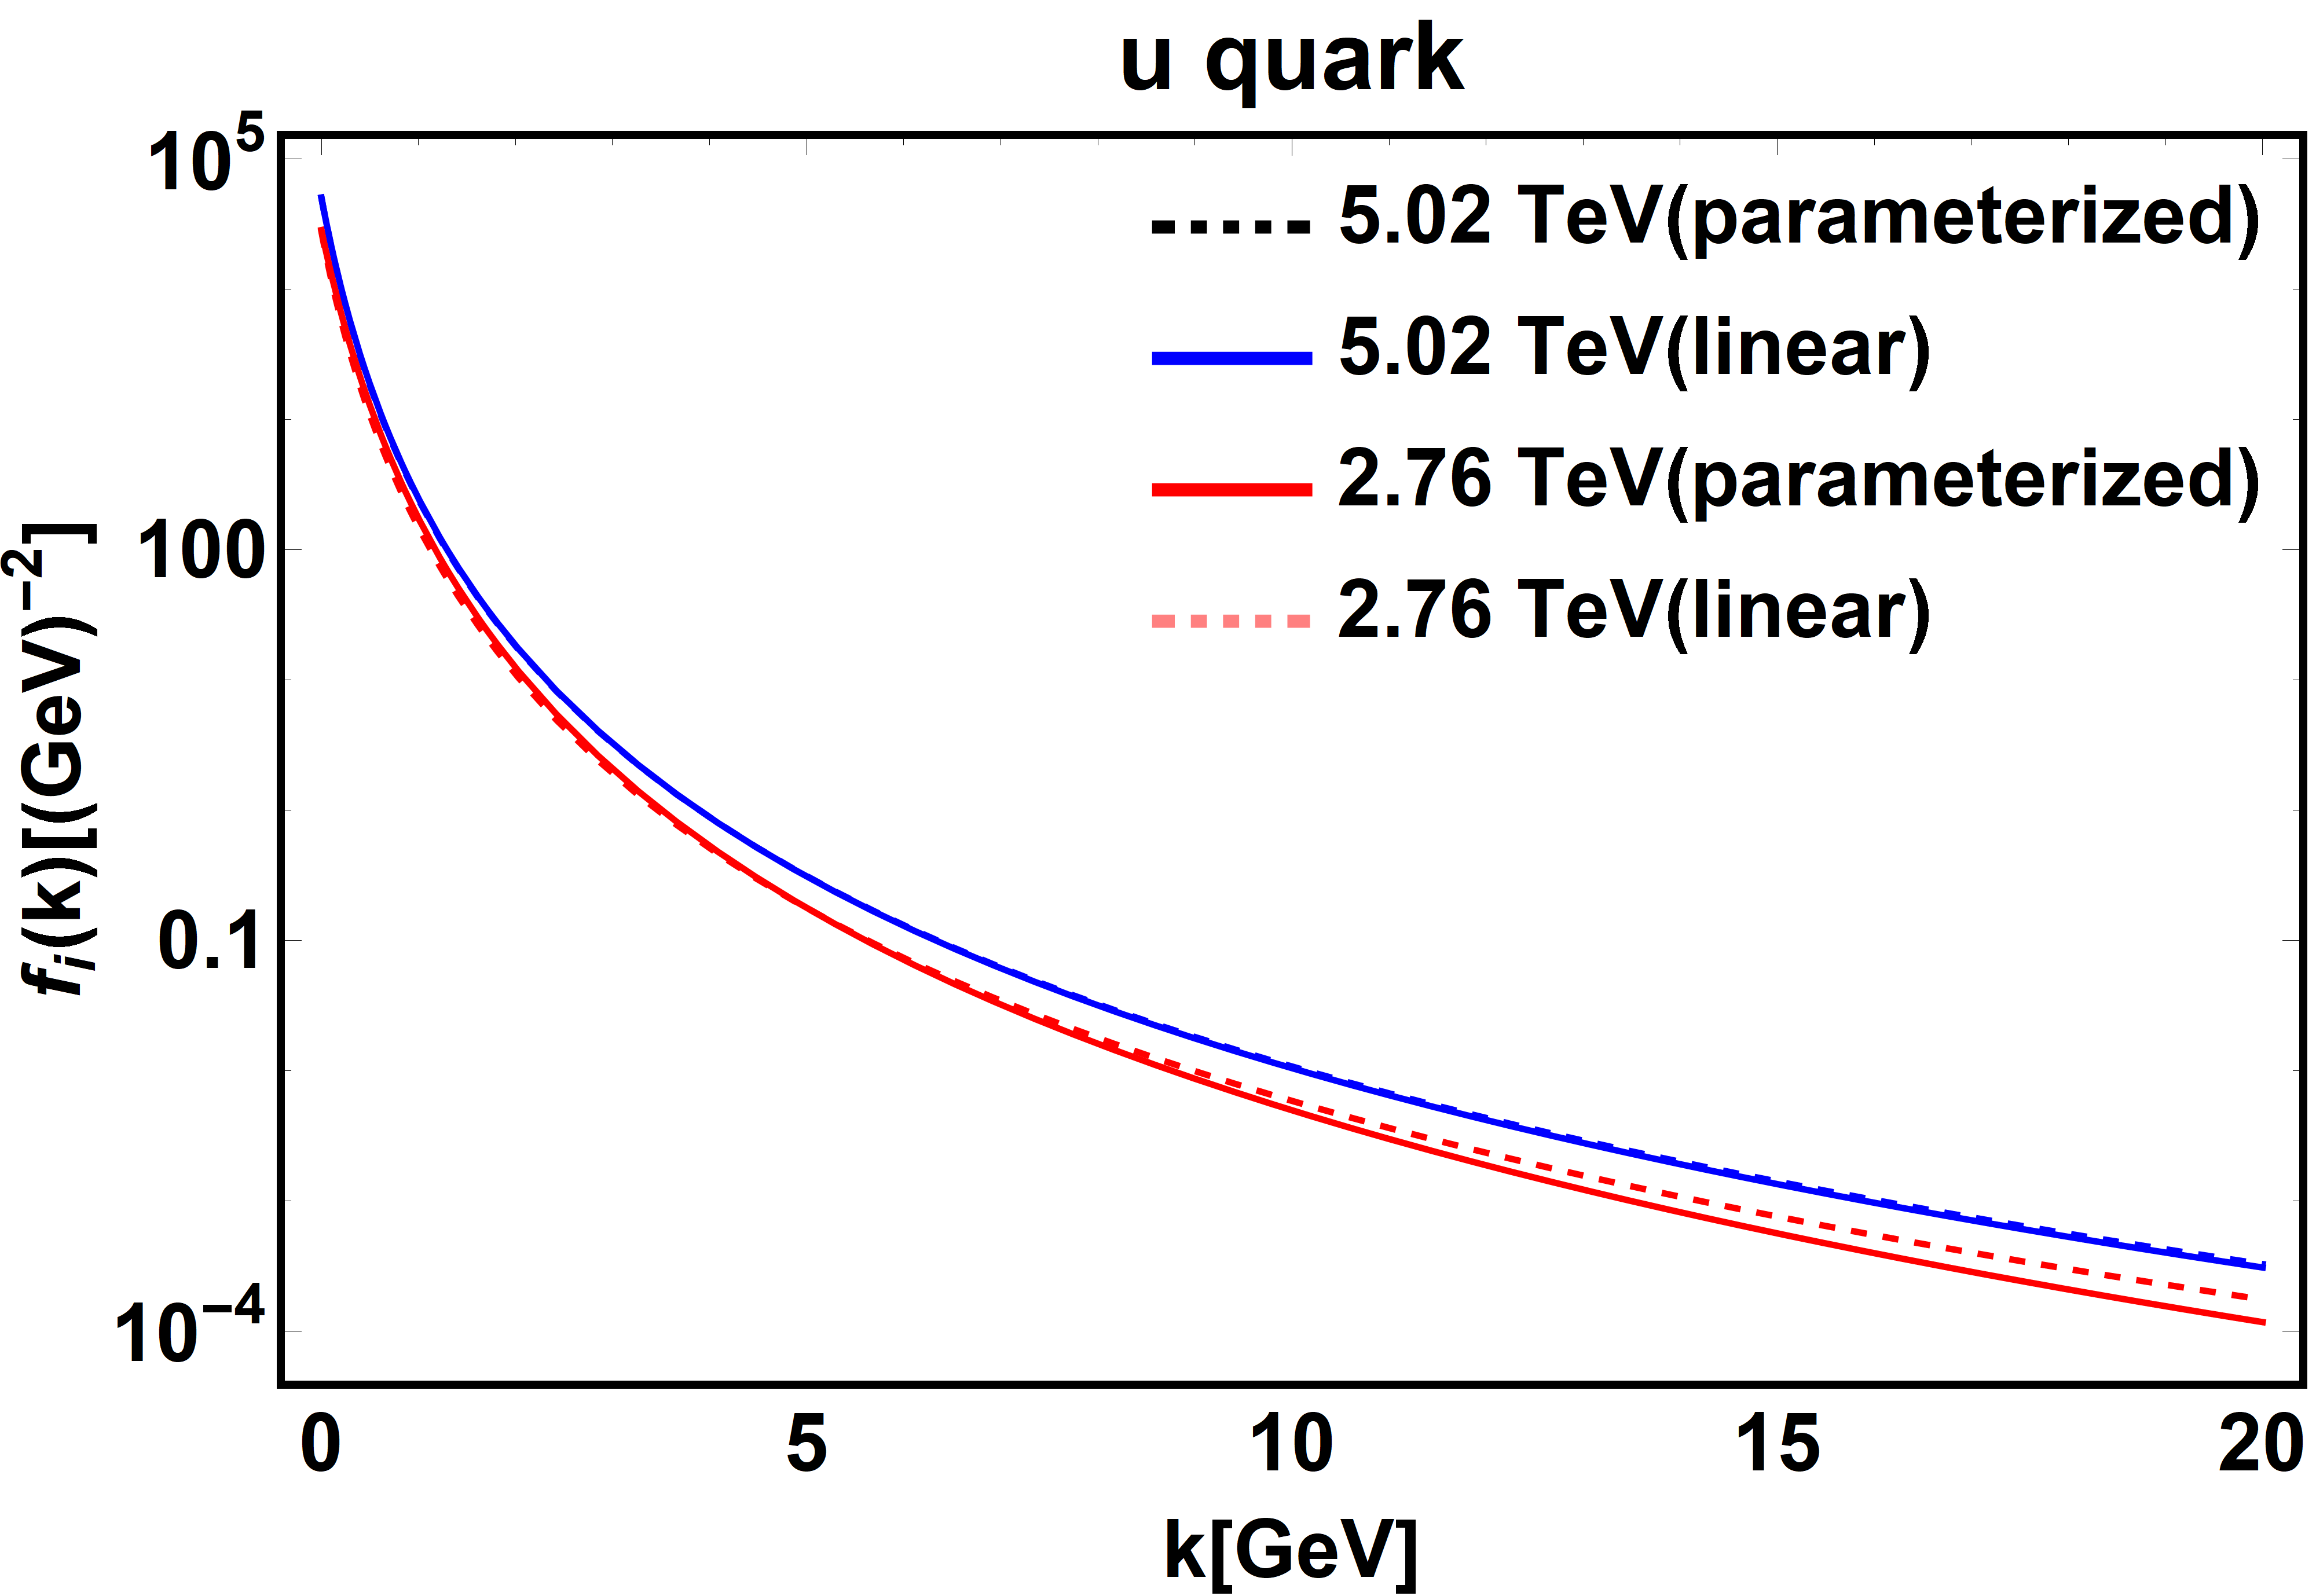
\includegraphics[width=0.45\textwidth]{compareu.png}
	\caption{Deviation between linear evaluation and parameterized values for u quark at 2.76 and 5.02 TeV.}
	\label{fig8}
\end{figure}

\begin{figure}[H]
	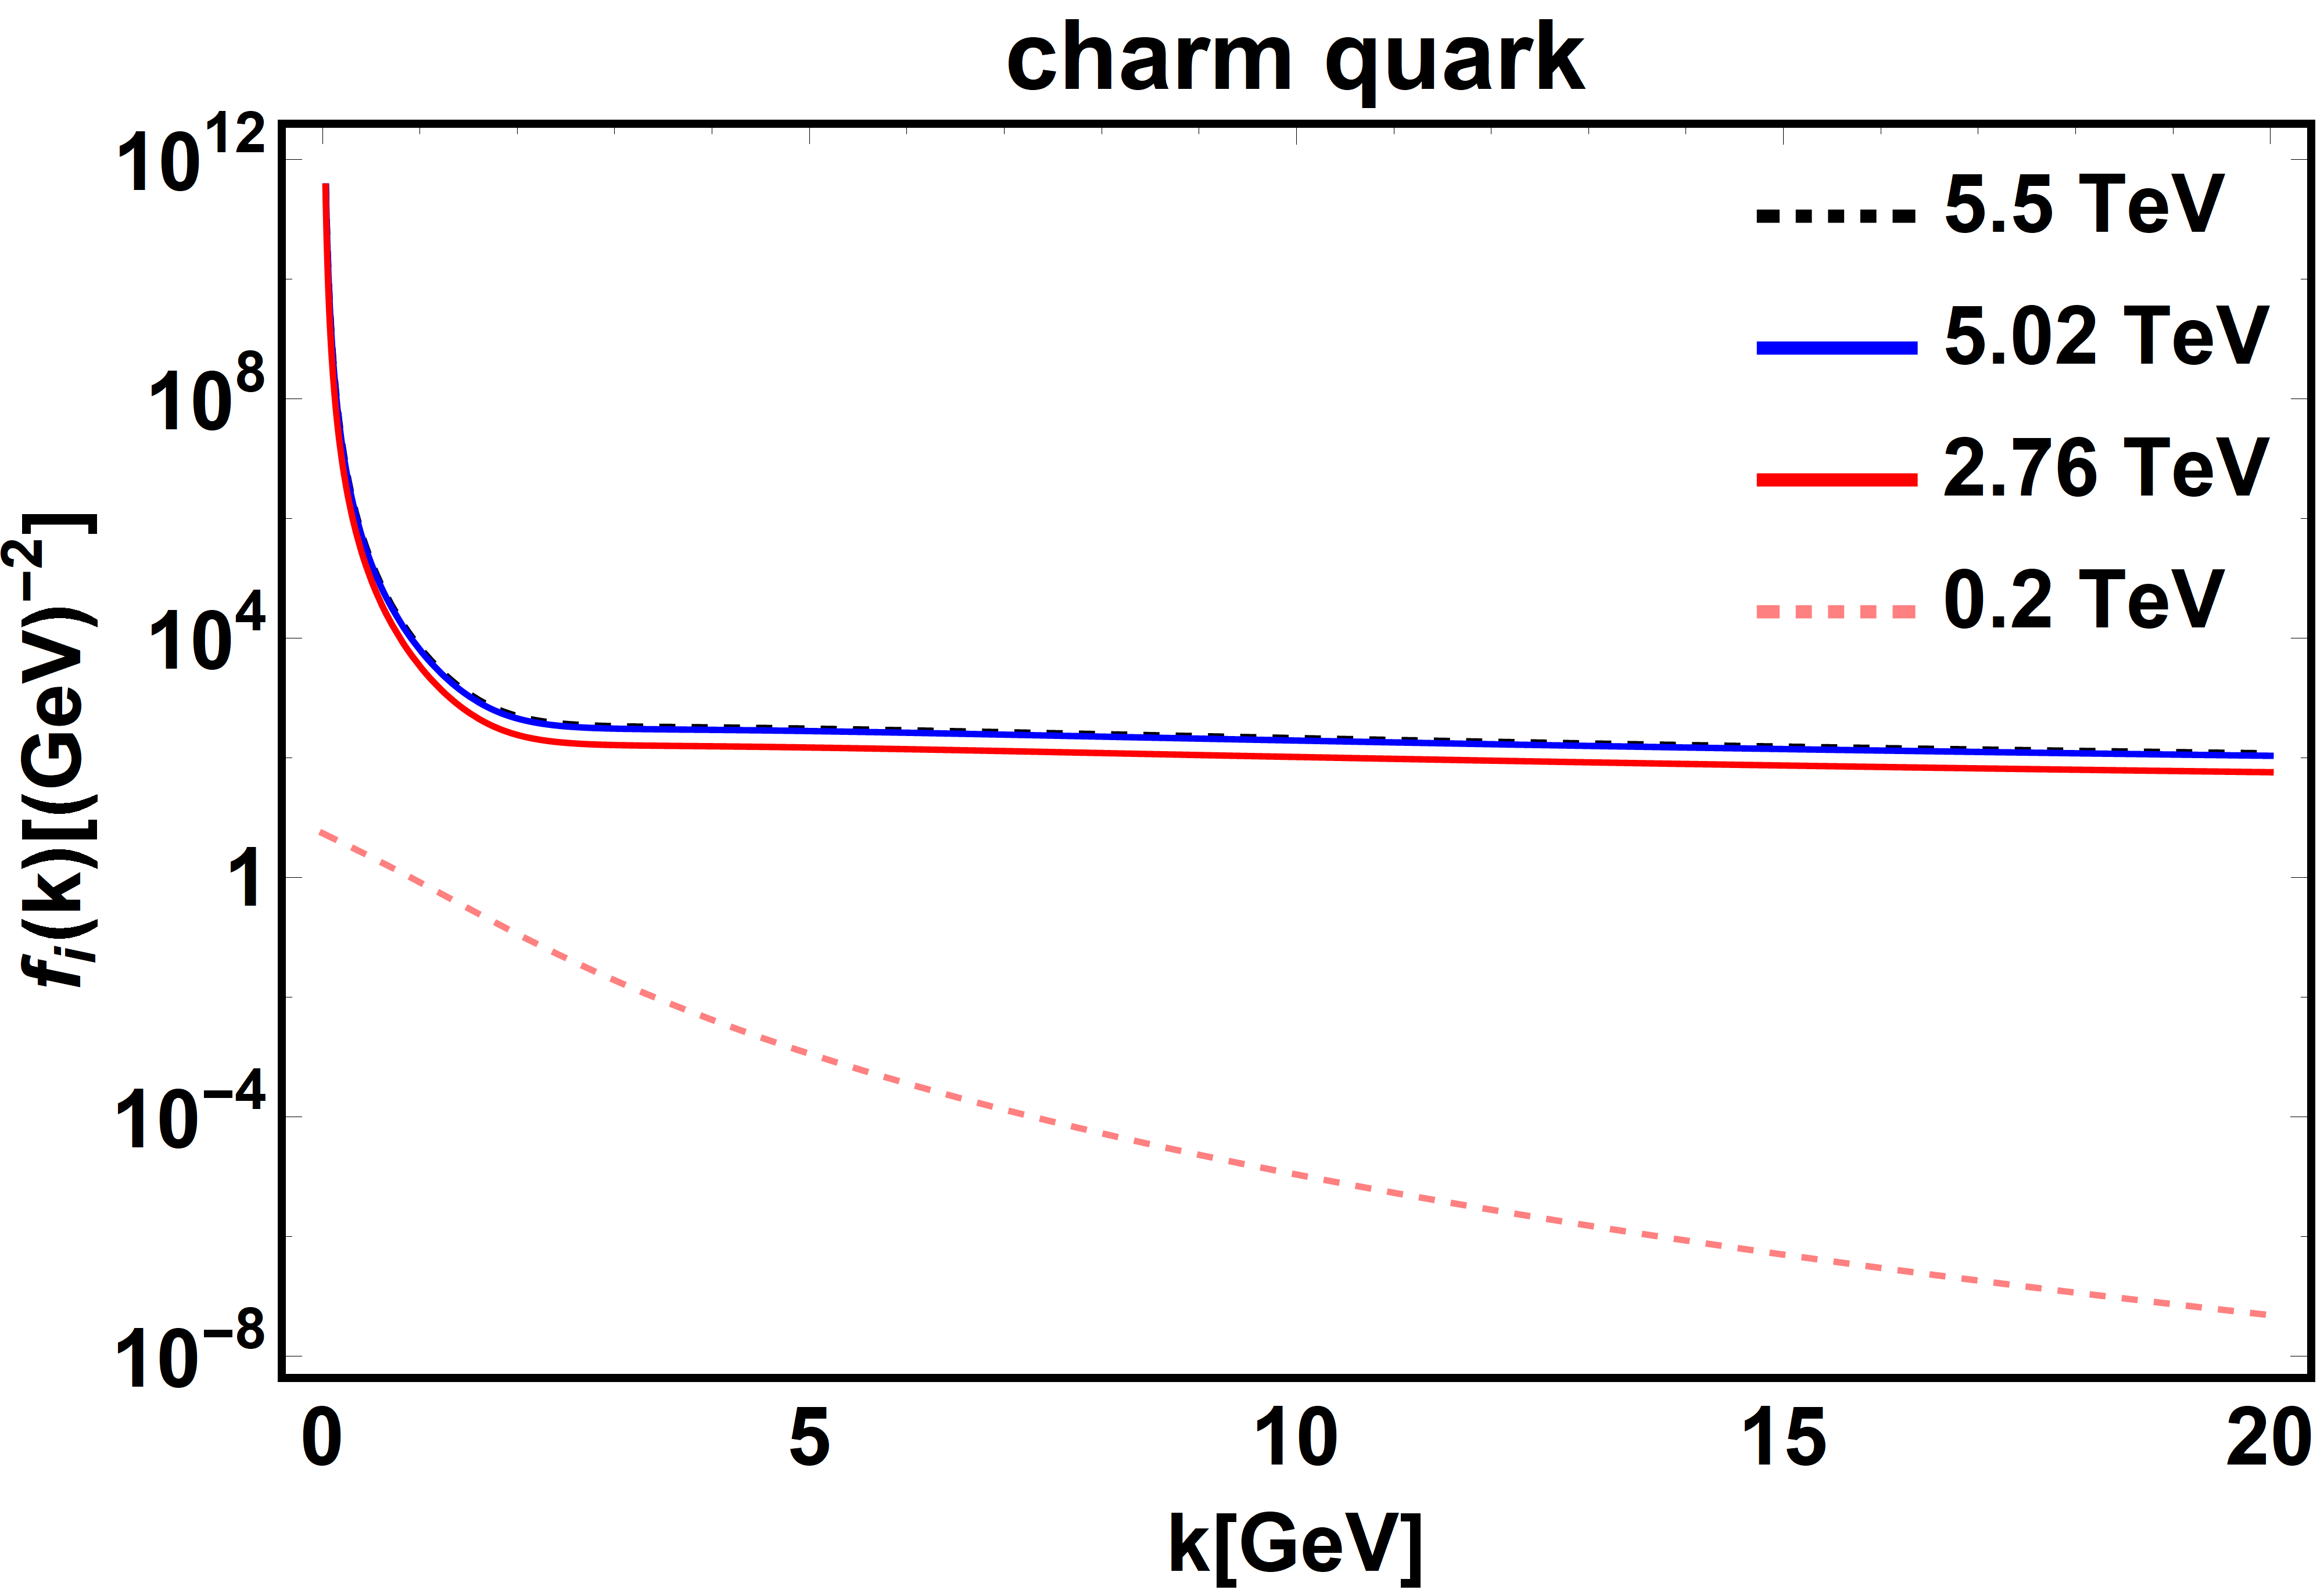
\includegraphics[width=0.45\textwidth]{fikc.png}
	\caption{Hard parton distribution of charm quark at various energy assuming $f_c(k)$ is linear with $\sqrt{s_{NN}}$.}
	\label{fig9}
\end{figure}

\begin{figure}[H]
	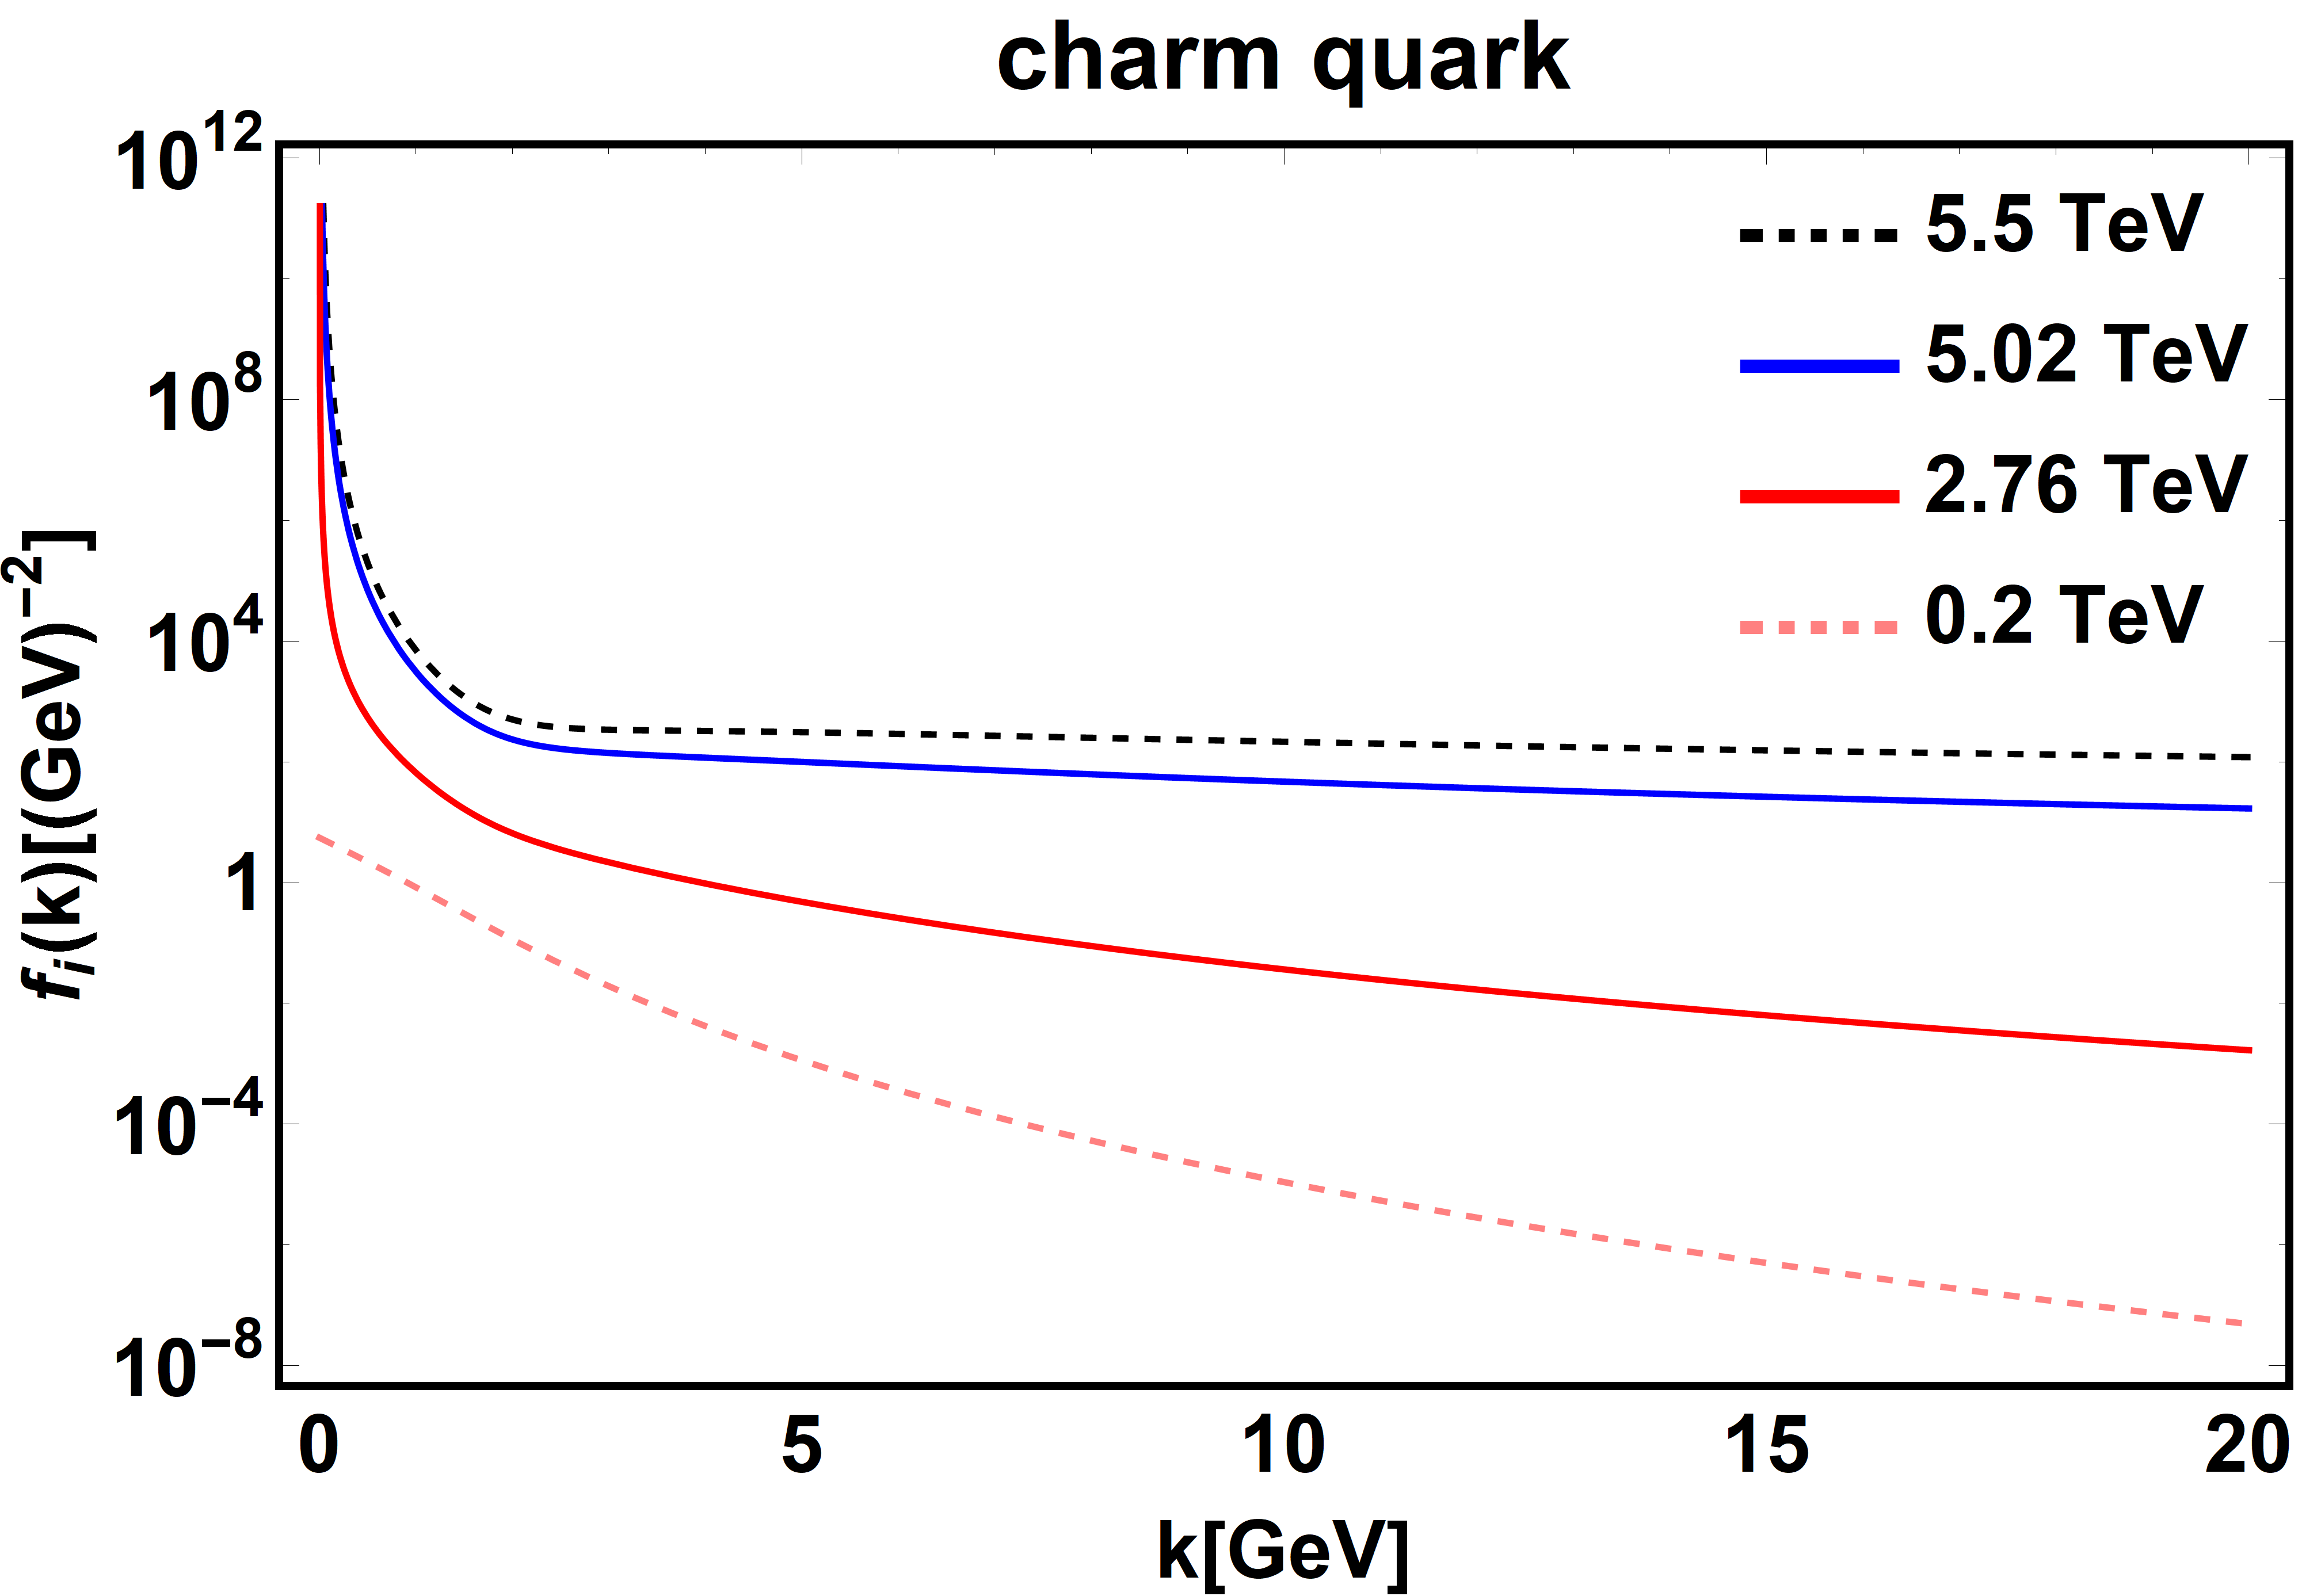
\includegraphics[width=0.45\textwidth]{fikc_log.png}
	\caption{Hard parton distribution of charm quark at various energy assuming $\ln(f_c(k))$ is linear with $\sqrt{s_{NN}}$.}
	\label{fig10}
\end{figure}

\begin{figure}[H]
	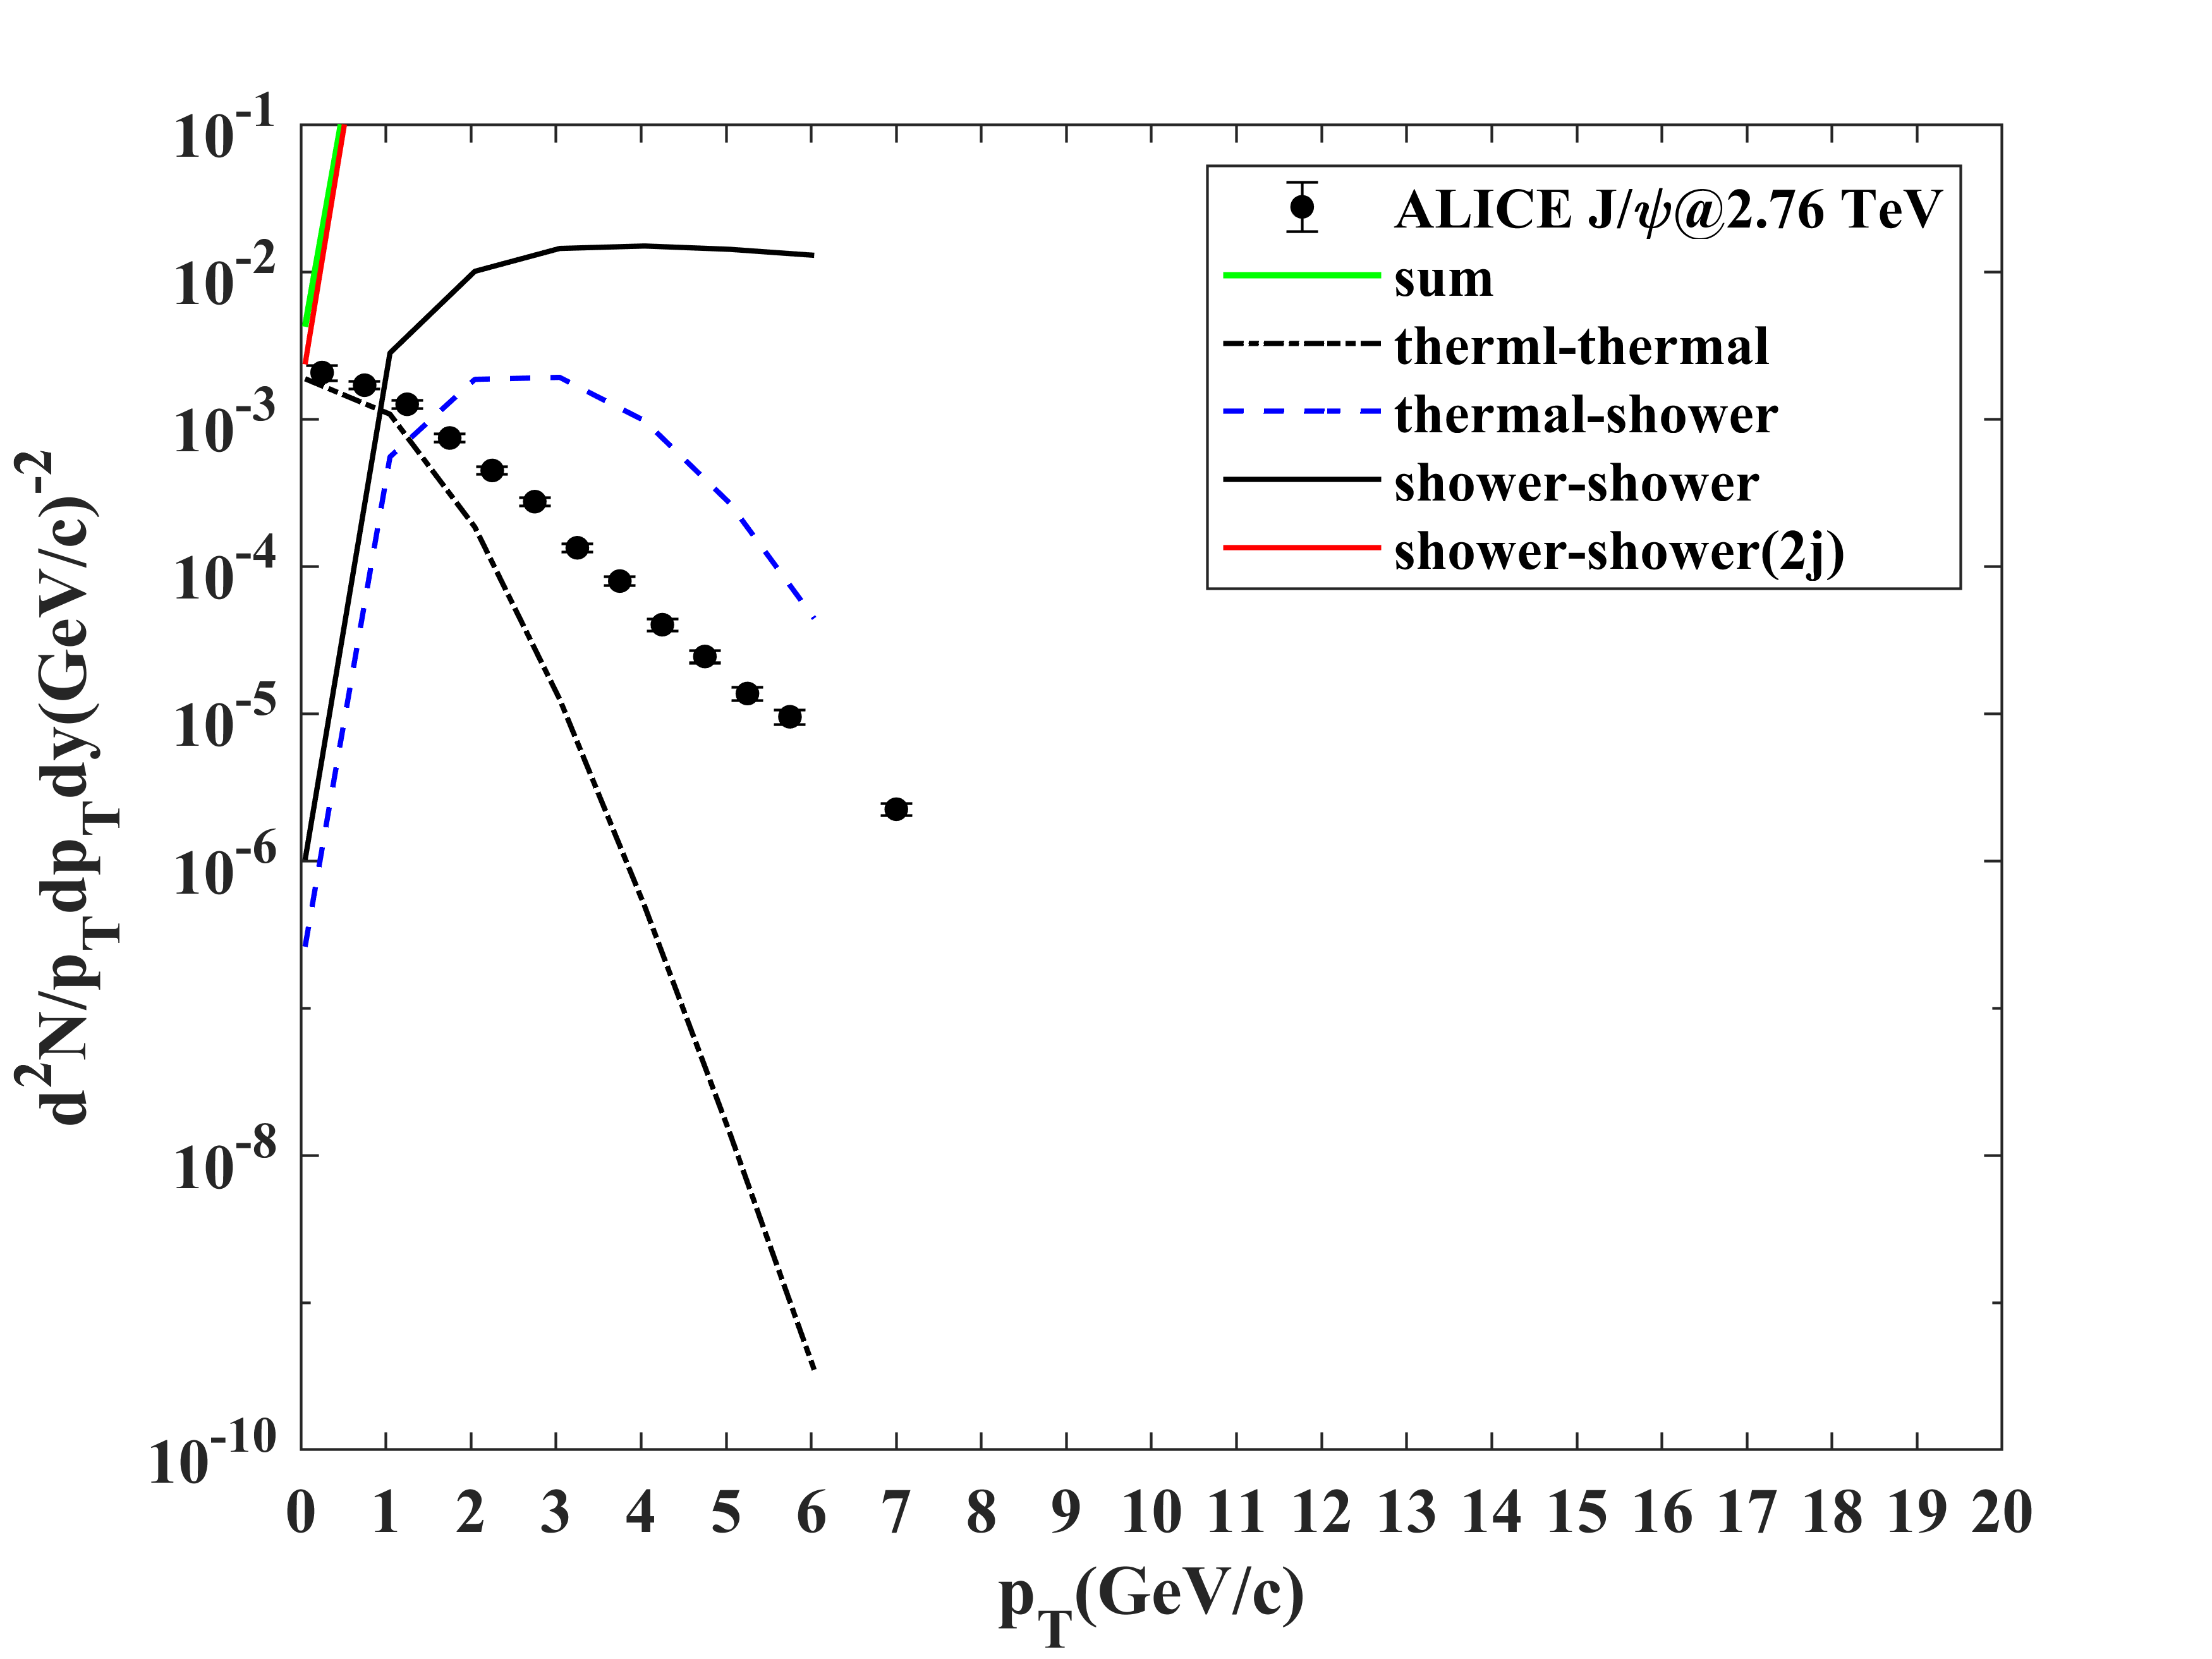
\includegraphics[width=0.45\textwidth]{jpsi_f_vs_s.png}
	\caption{$J/\psi$ distribution at 2.76 TeV assuming $f_c(k)$ is linear with $\sqrt{s_{NN}}$.}
	\label{fig12}
\end{figure}

\begin{figure}[H]
	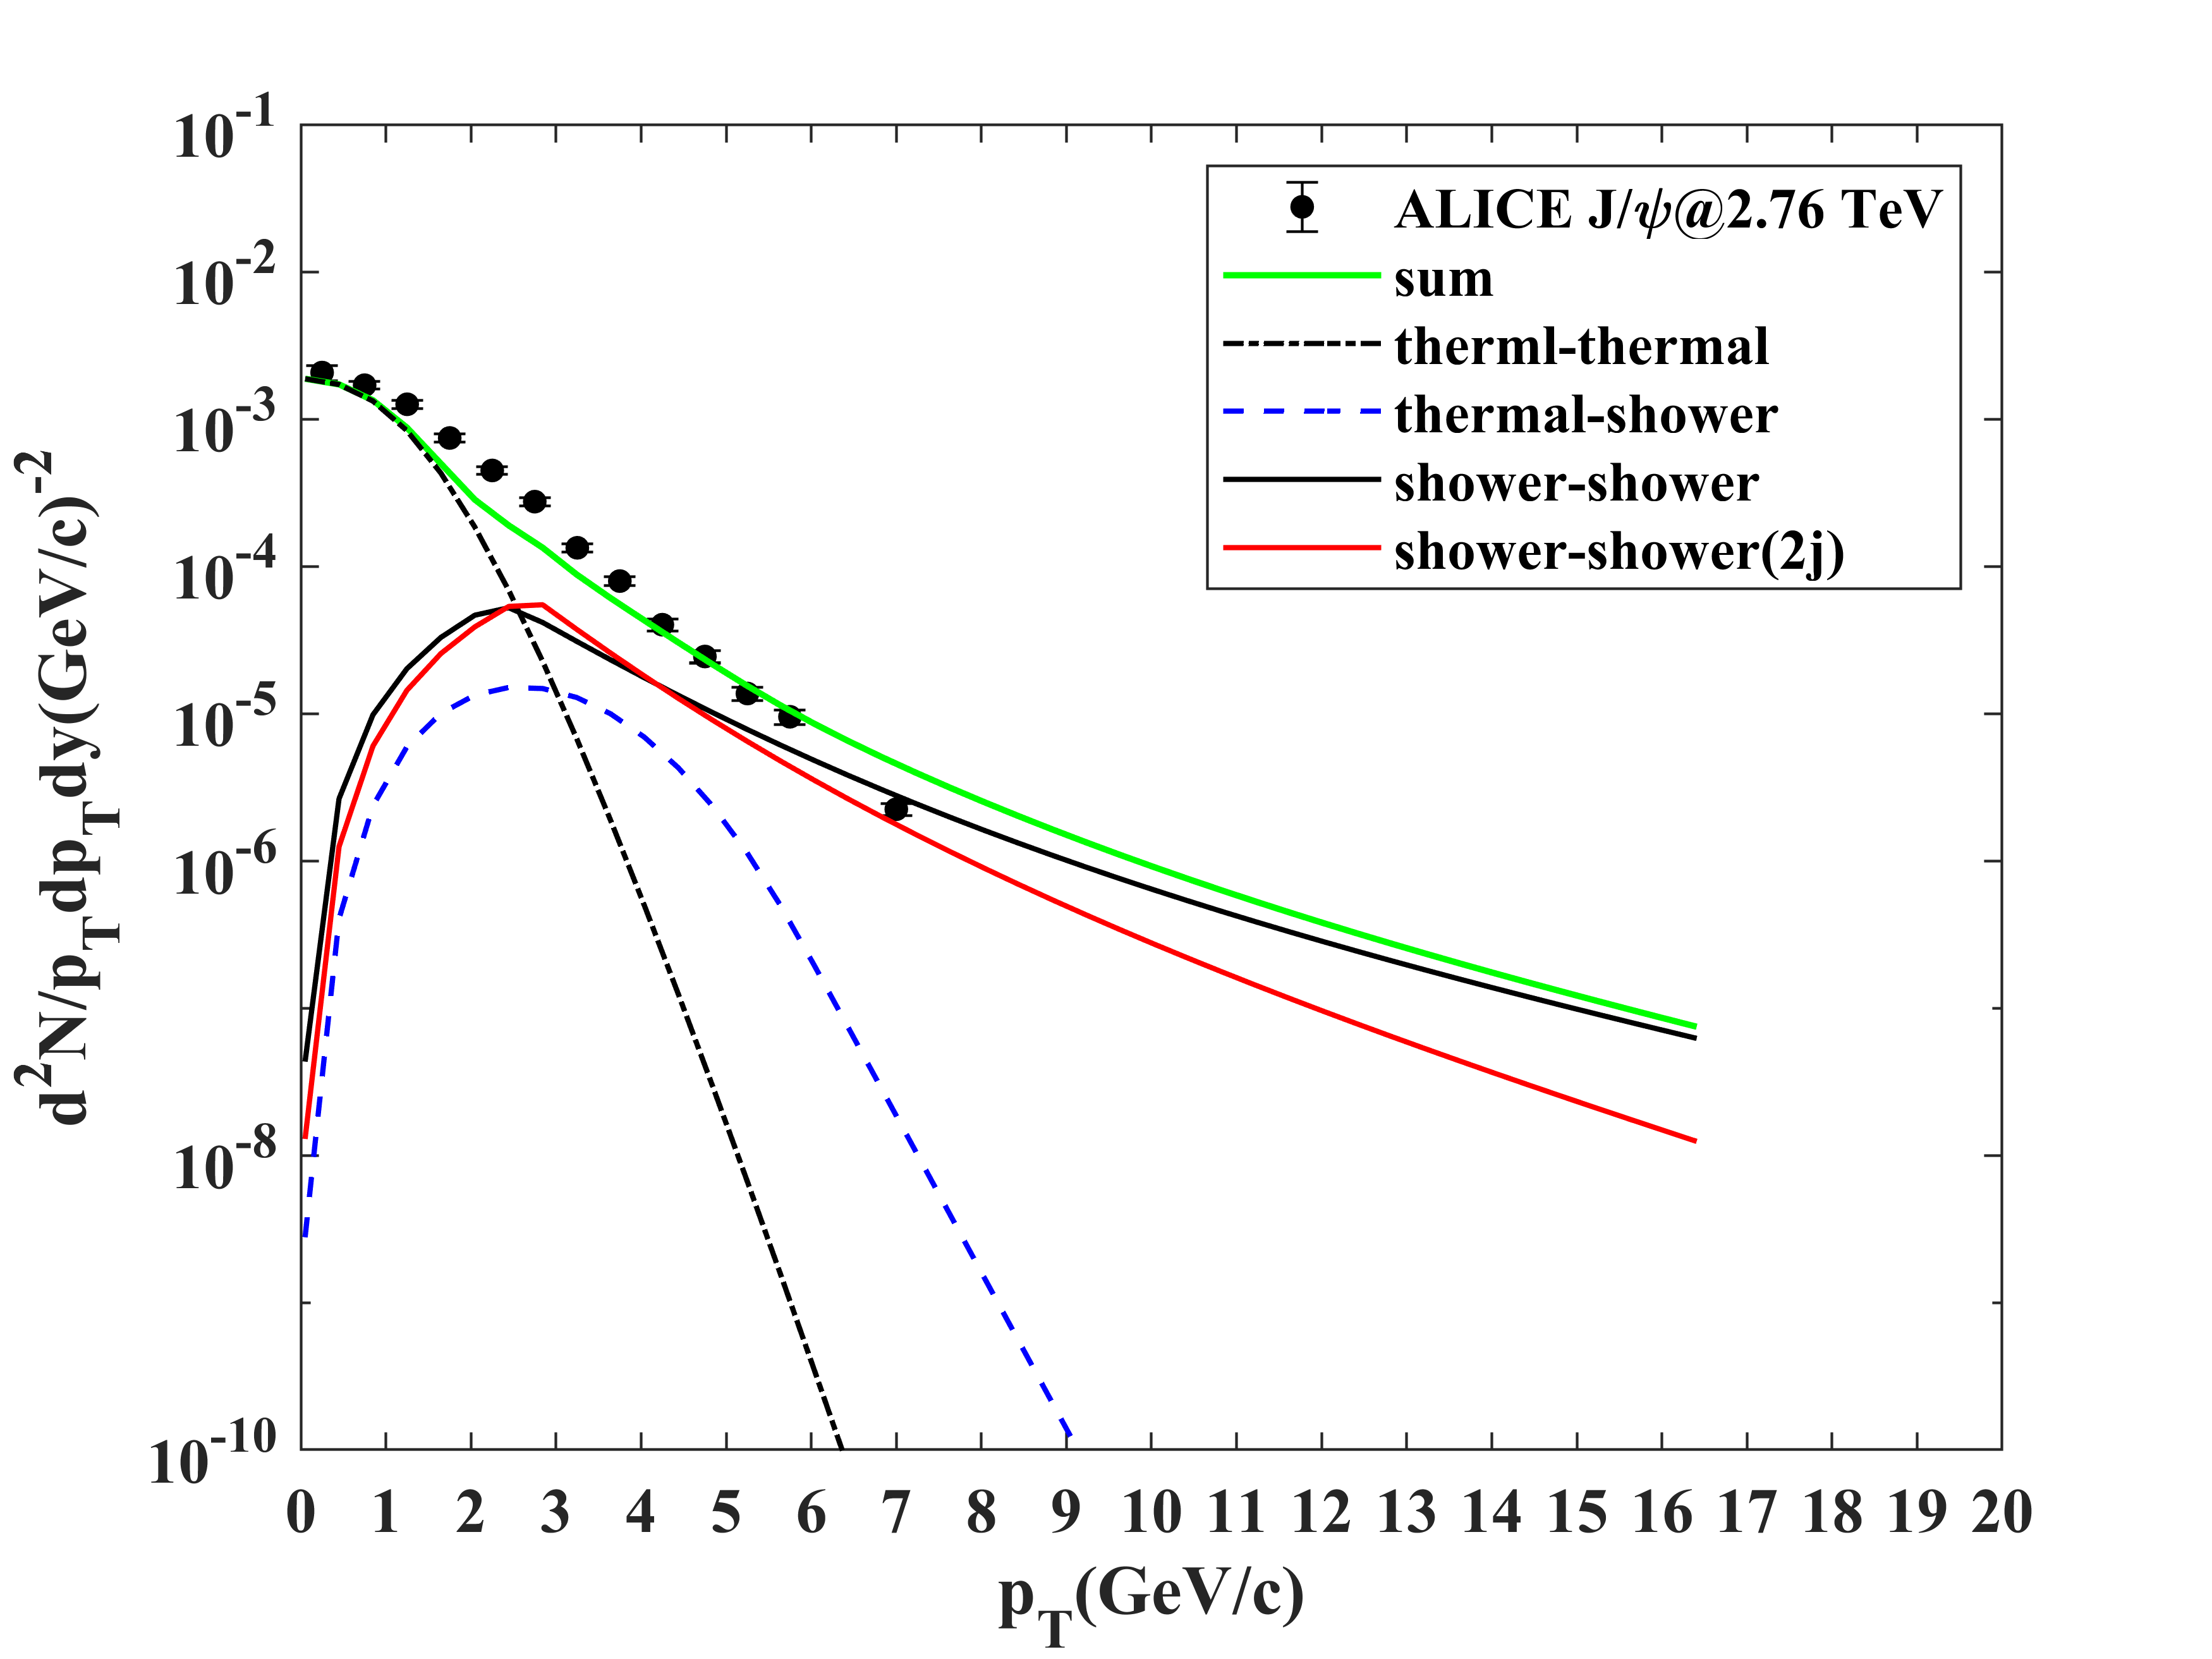
\includegraphics[width=0.45\textwidth]{jpsi_lnf_vs_s.png}
	\caption{$J/\psi$ distribution at 2.76 TeV assuming $f_c(k)$ is exponential with $\sqrt{s_{NN}}$.}
	\label{fig13}
\end{figure}

\begin{figure}[H]
	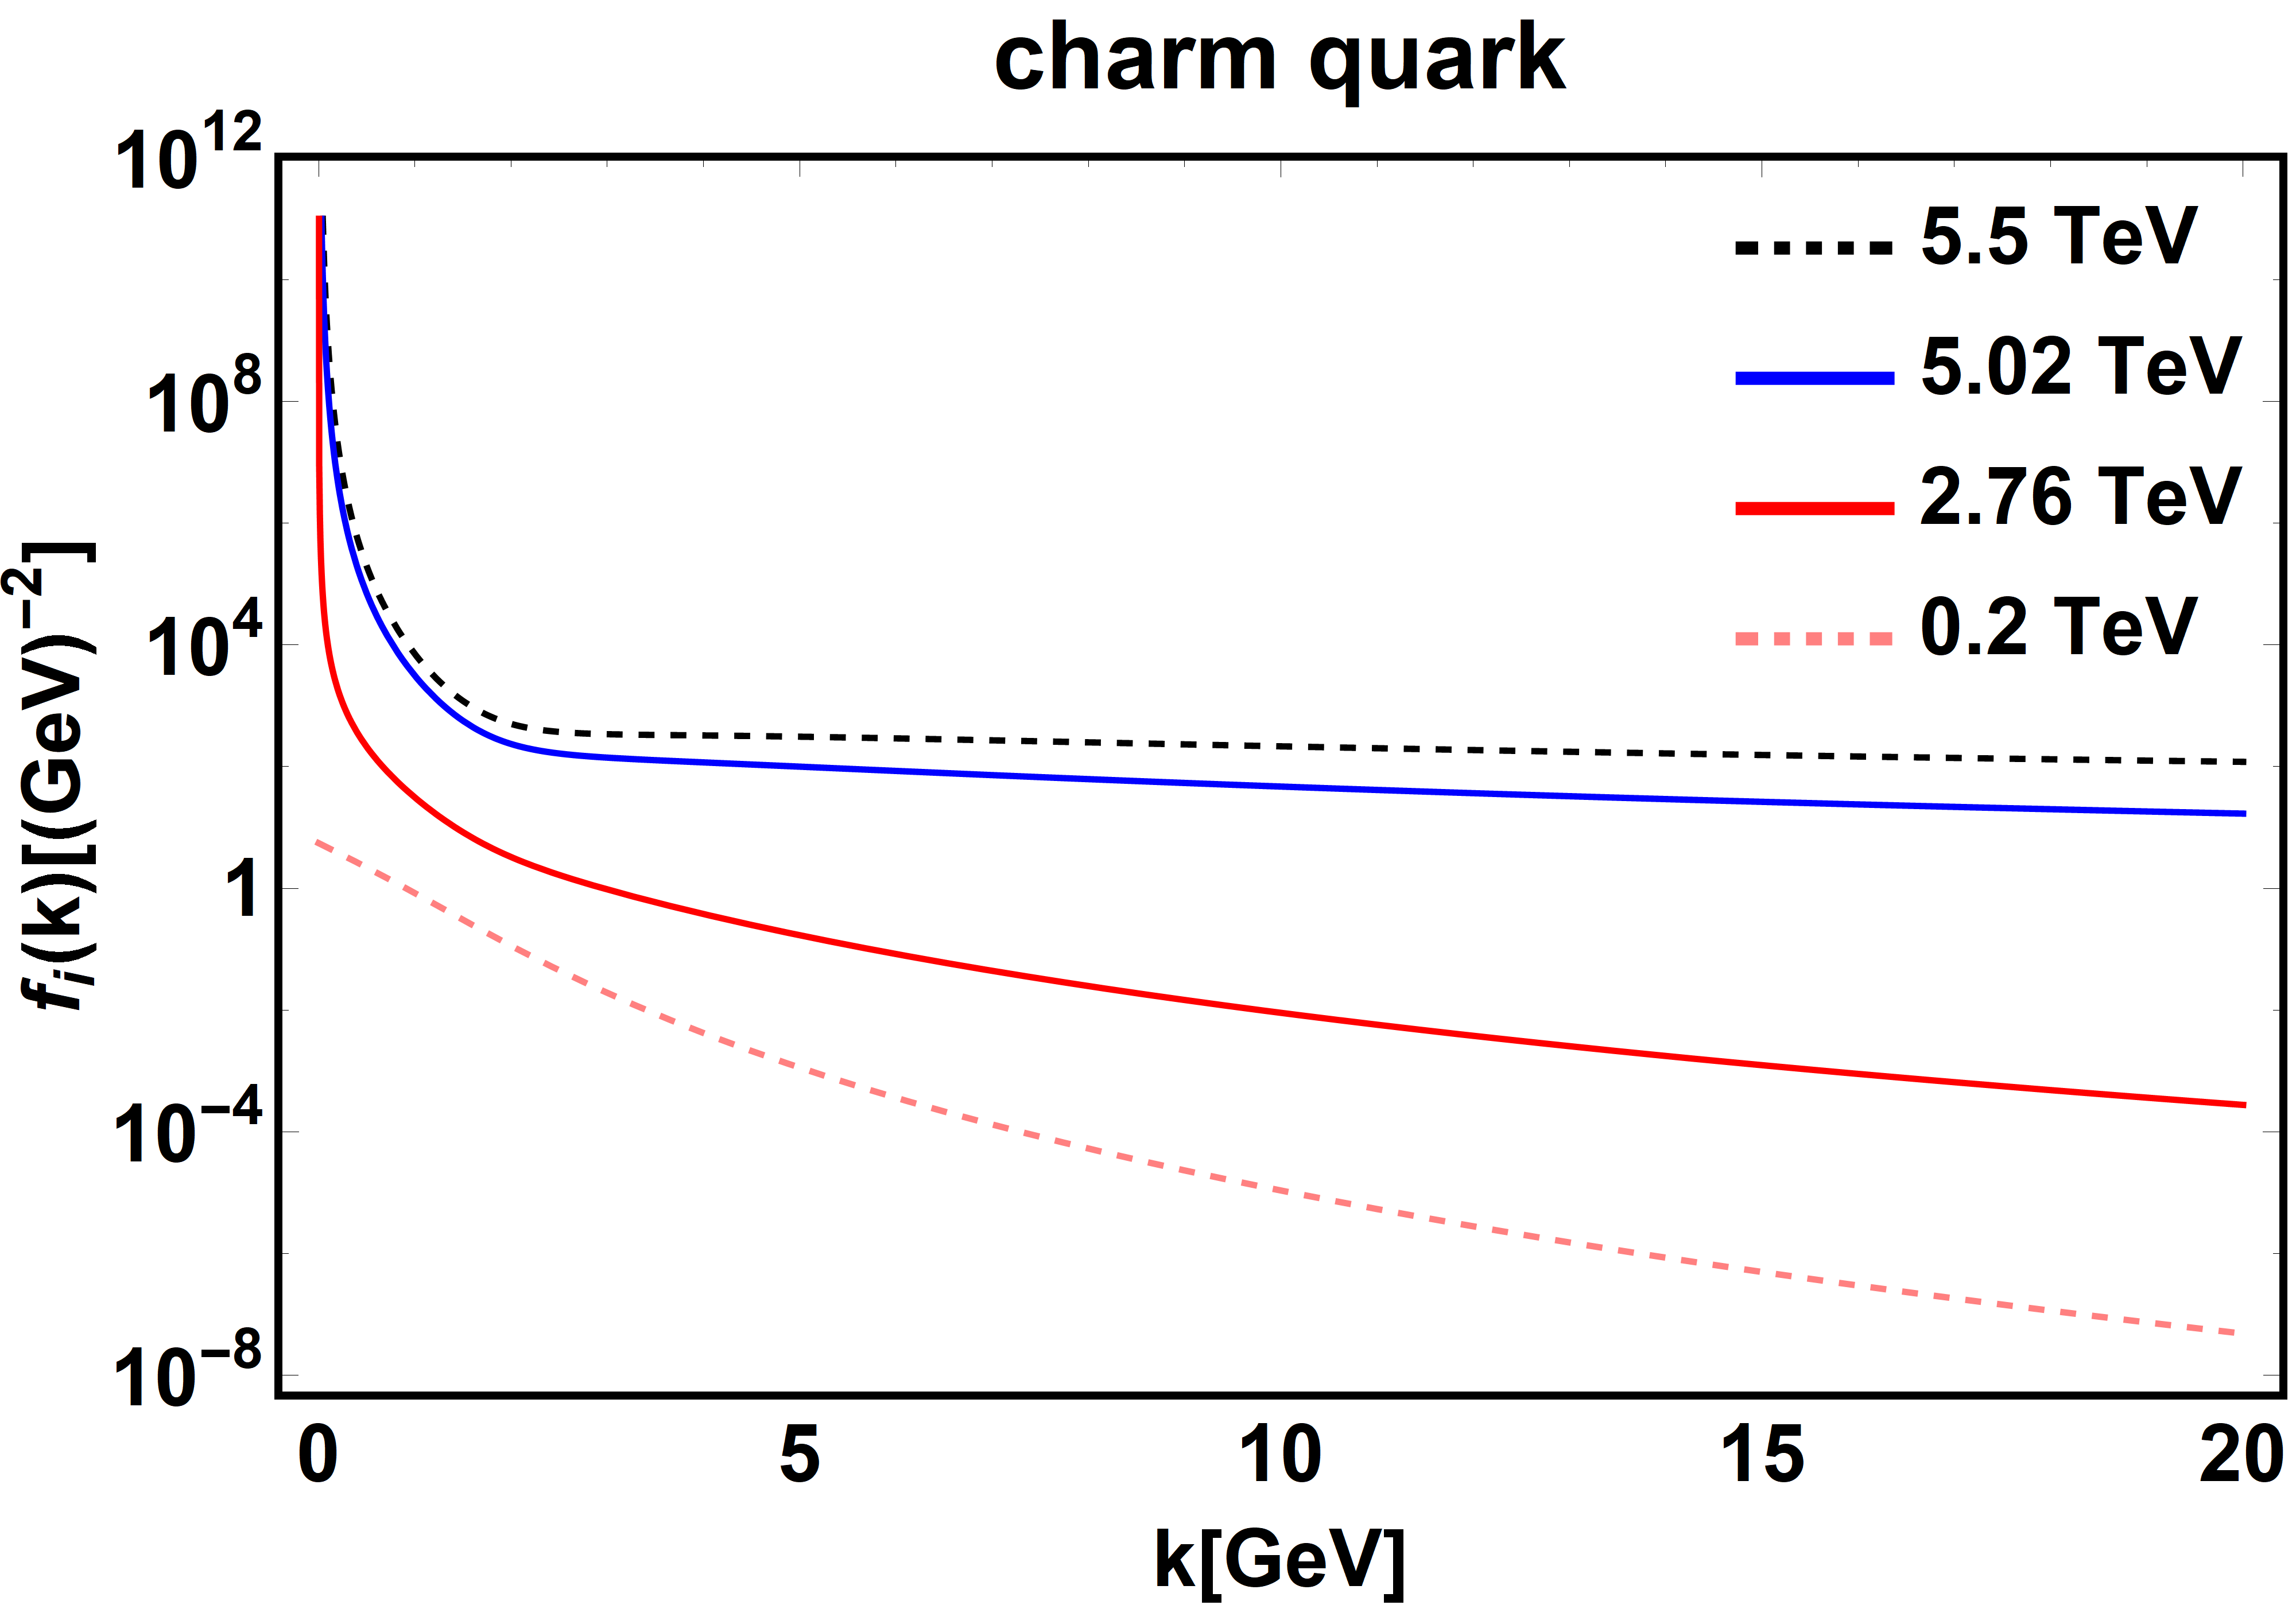
\includegraphics[width=0.45\textwidth]{improved fck.png}
	\caption{Hard parton distribution of charm quark at various energy assuming $f_c(k)$ =0.6$f^{0.2}_c(k)$+0.4$f^{5.5}_c(k)$.}
	\label{improved fck}
\end{figure}

\begin{figure}[H]
	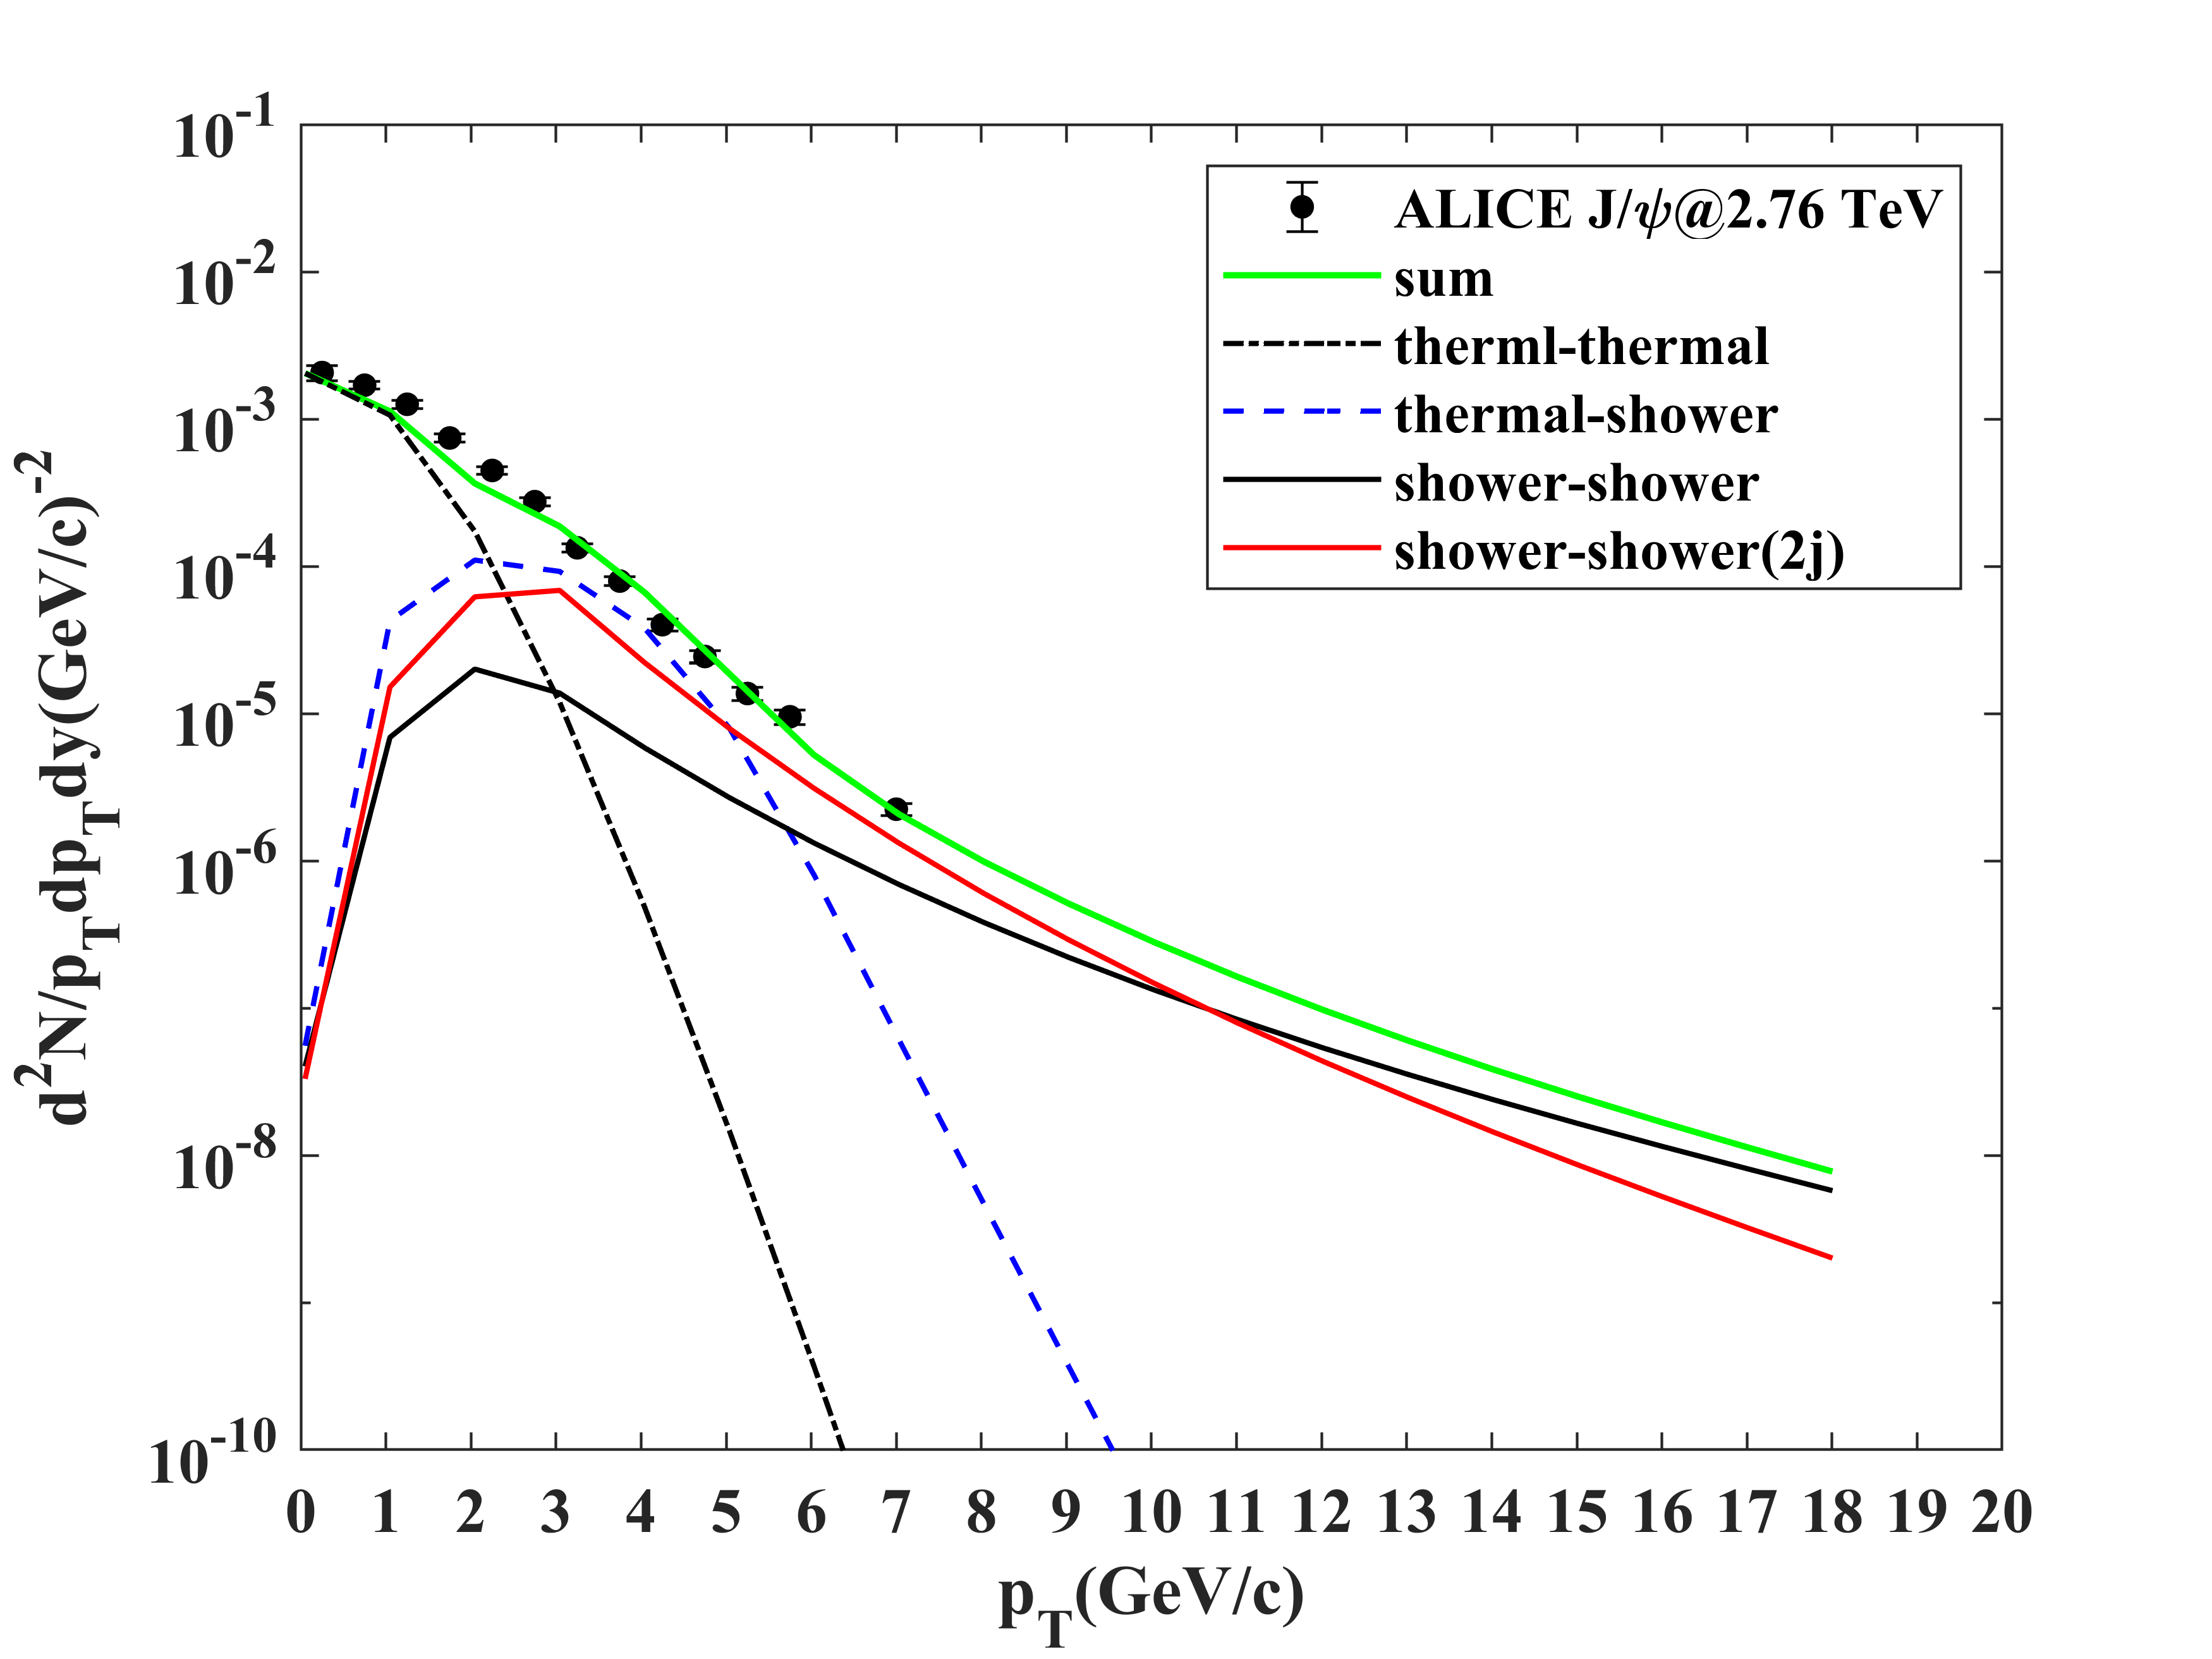
\includegraphics[width=0.45\textwidth]{Jpsi_276_4th.png}
	\caption{$J/\psi$ distribution at 2.76 TeV applying improved $f_c(k)$.}
	\label{fig14}
\end{figure}

\begin{figure}[H]
	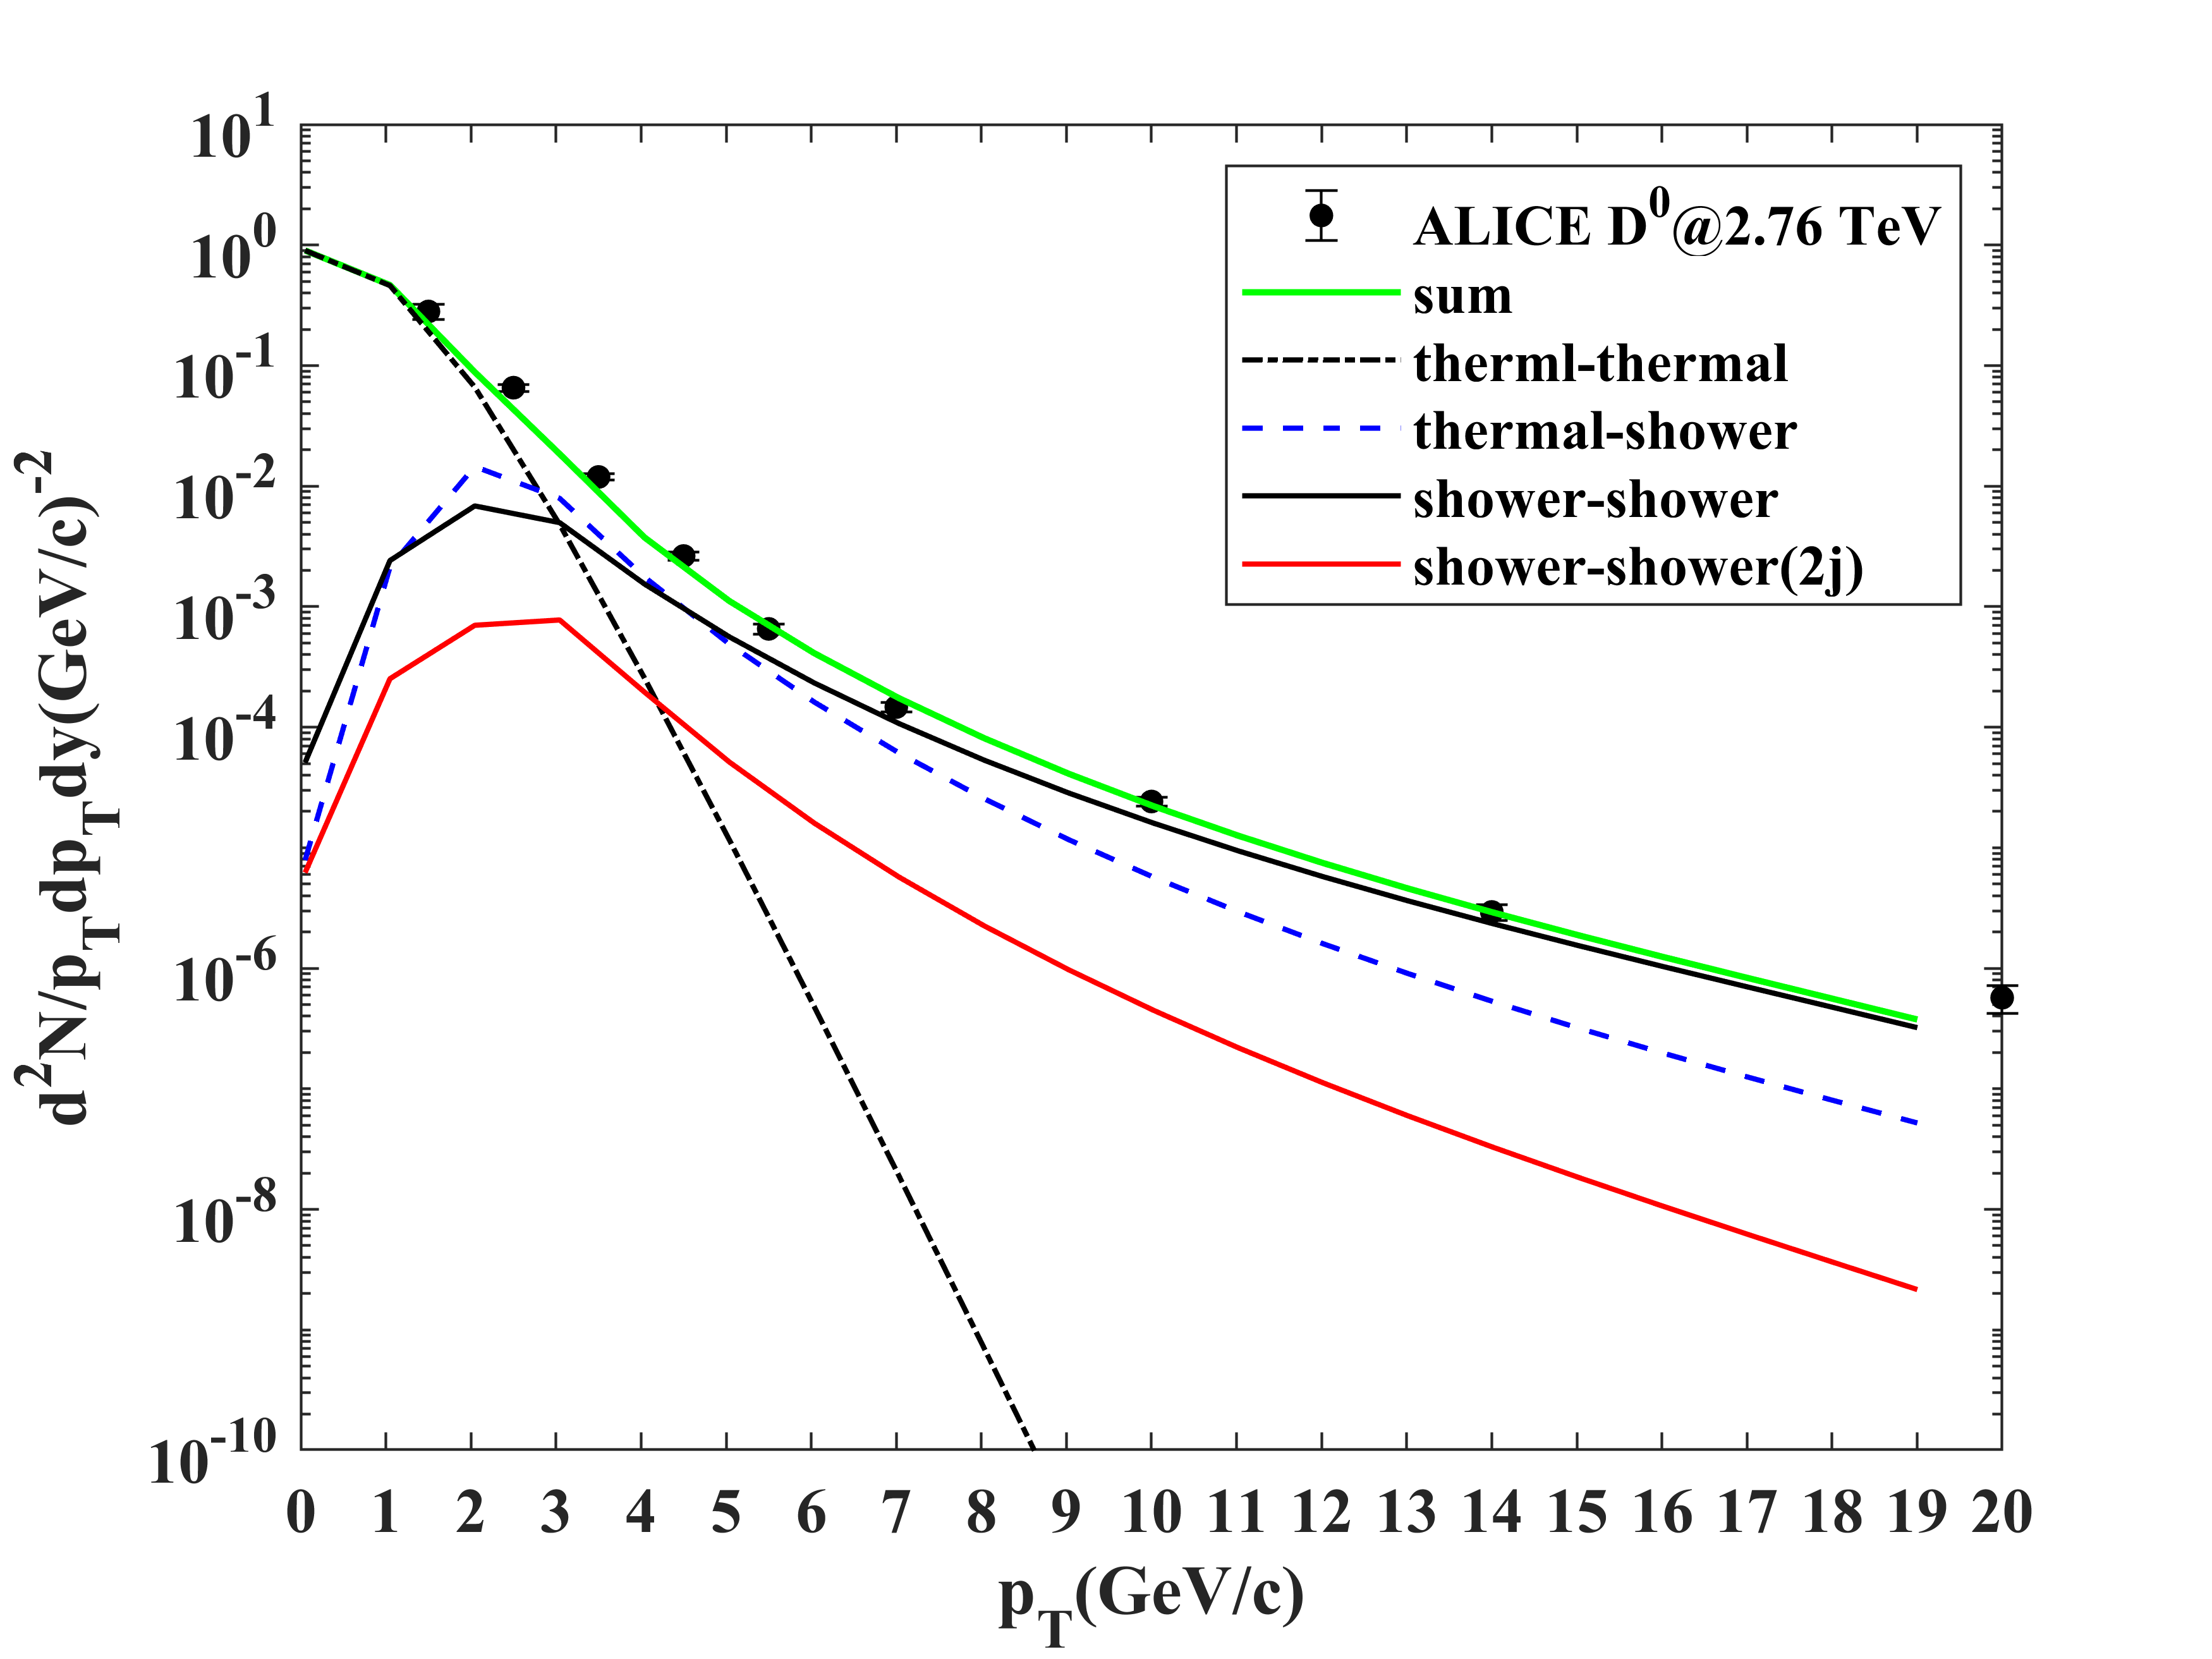
\includegraphics[width=0.45\textwidth]{D0_276_final.png}
	\caption{$D^0$ distribution at 2.76 TeV applying improved $f_c(k)$.}
	\label{fig15}
\end{figure}

\begin{figure}[H]
	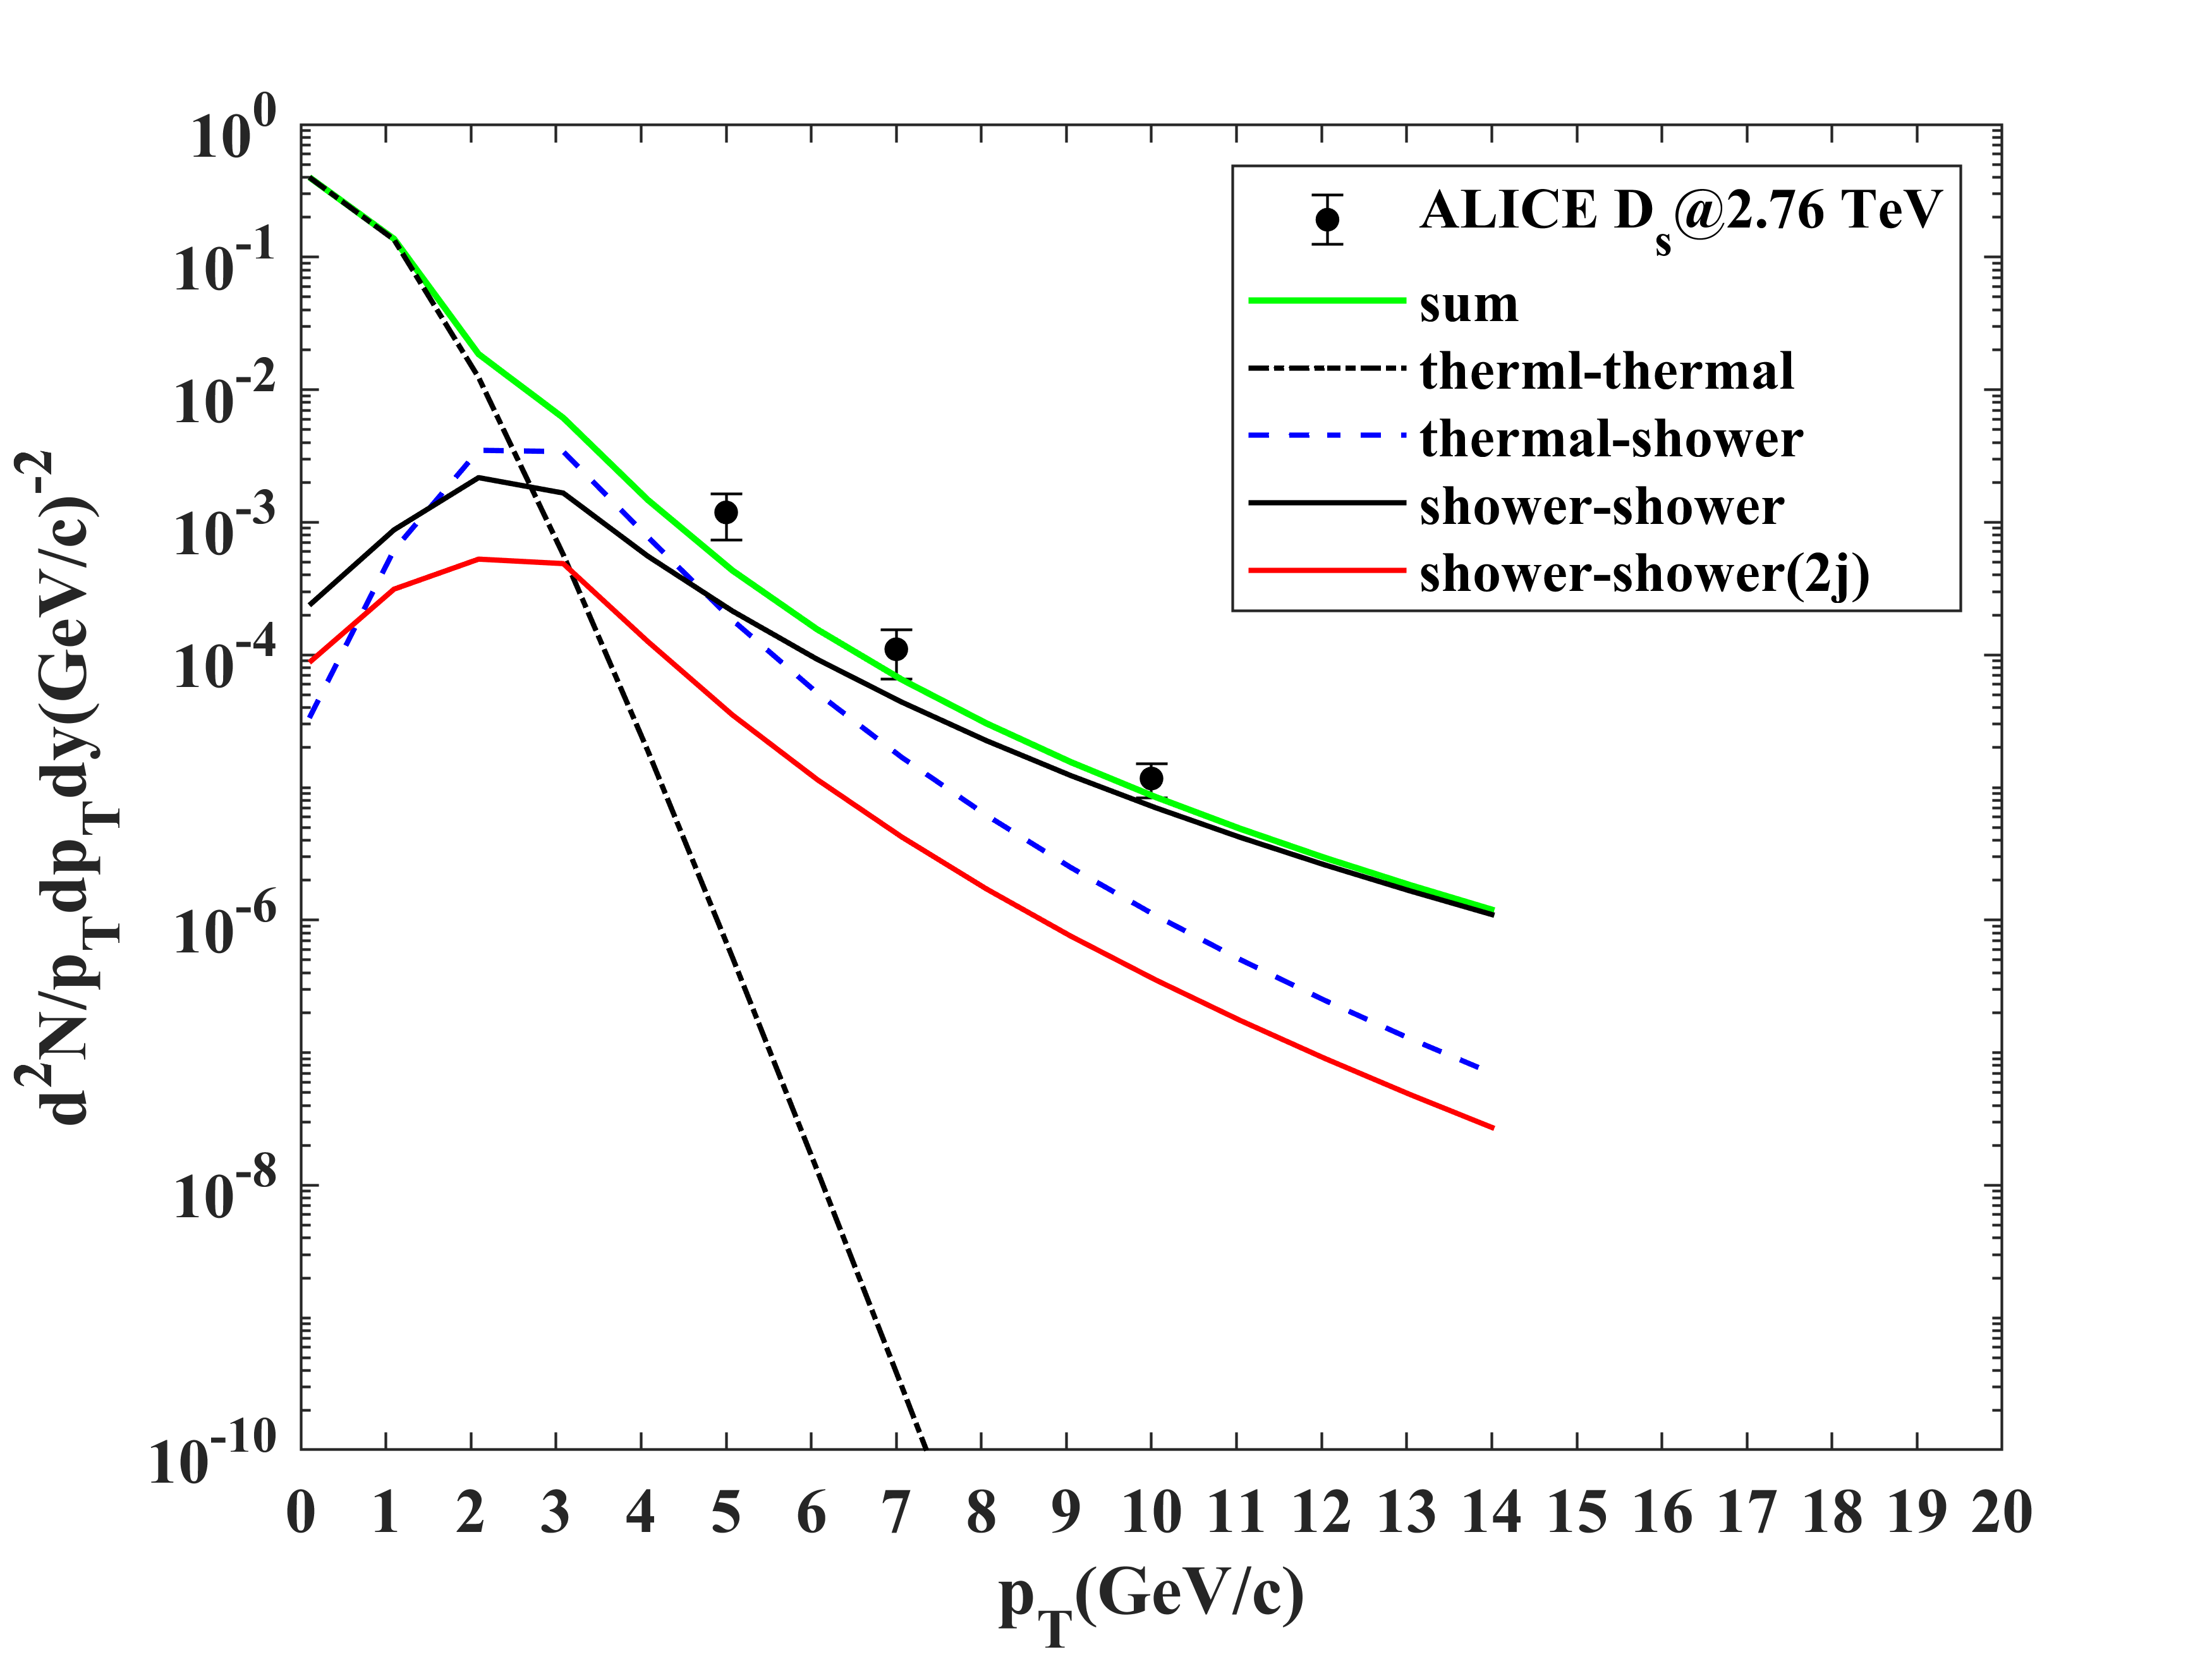
\includegraphics[width=0.45\textwidth]{Ds_276_final.png}
	\caption{$D_s$ distribution at 2.76 TeV applying improved $f_c(k)$.}
	\label{fig16}
\end{figure}

\section{Meeting 2022.10.24}
Last week, we improved the program by adopting $R_{J/\psi}={x_1 x_2\over x^2}\delta({x_1+x_2 \over x}-1)$ instead of ${x_1 x_2\over x^2} \delta({x_1\over x}-{1\over 2}) \delta({x_2\over x}-{1\over 2})$ owing to interaction between $c$ and $\overline{c}$ quark. However, now we still adopt the latter form and $m_c=1.5$ GeV to be consistent with Ref.\cite{Peng:2011zzd}. Moreover, we should limit the $p_T$ spectra in the range of 0 to 10 GeV to raise the program operating speed. 

Besides, we fix the hard jet momentum limits $q$ in shower parton distribution in the range of after checking $\itshape{recomb\_product\_v15.f90}$. Next we will improve the $SS(1)$ term and reproduce $J/\psi, D^0, D_s$ at 2.76 and 5.02 TeV, and figure out the issue of $SS(2)$ which shows a sharp decrease at point of changing integration low limit in Fig.\ref{fig17}.
\begin{figure}[H]
	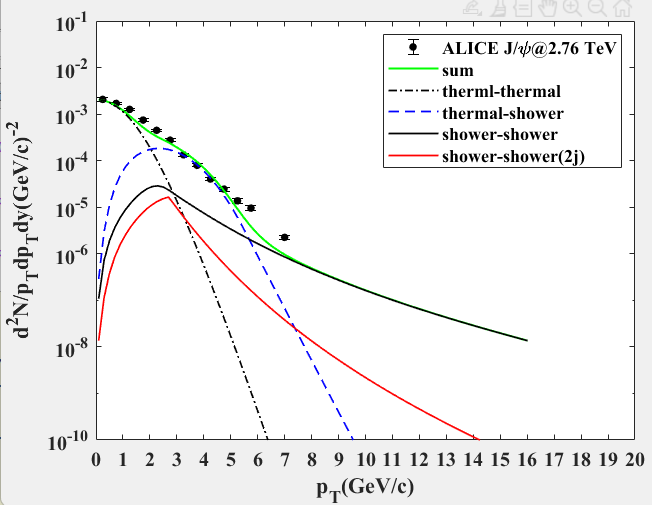
\includegraphics[width=0.45\textwidth]{Jpsi_221024.png}
	\caption{$J/\psi$ distribution at 2.76 TeV at 2022/10/24 meeting.}
	\label{fig17}
\end{figure}

\section{Meeting 2022.10.31}
Last week, we attempt to fit $TT$ and $TS$ terms by adopting $R_{J/\psi}={x_1 x_2\over x^2} \delta({x_1\over x}-{1\over 2}) \delta({x_2\over x}-{1\over 2})$ and $m_c=1.5$ GeV. However, we find it hard to fit so we still use $m_c=1.28$ GeV and change $R_{J/\psi}$ back only. Then, we improve the integrate limits in Eq.\ref{ss2_jpsi} from 3 to 15 GeV and the critical point is changed to $p_T=2q$. 

Besides, trying to add cutoff in reference of \cite{Zhu_2020} and \cite{Zhu_cutoff}, we find it analogous to add either $1-e^{-p/2}$ or the cutoff. It is much lower if two factor are both added to  suppress the low $p_T$ contribution. Therefore, the cutoff are abandoned. 

This week, $J/\psi$ distribution is improved, shown in Fig.\ref{fig18}, in which parameters at 2.76 TeV are listed here in comparison with them at 200 GeV:
\begin{eqnarray}
	J/\psi \text{ at 2.76 TeV}&:& v_T=0.25c, \gamma_c=0.26,\\
	 &&T=0.185 \text{ GeV}, \Gamma=10^{-2},  \nonumber \\
	&&\beta L\rightarrow \text{0 for charm, 2.39 for gluon.} \nonumber\\
	J/\psi \text{ at 200 GeV}&:& v_T=0.3c, \gamma_c=0.26,\\
	&&T=0.175 \text{ GeV},  \nonumber \\
	&&\beta L\rightarrow \text{0 for charm, 2.39 for gluon.}\nonumber
\end{eqnarray}
The results have a good agreement with ALICE data. And we will begin to focus on $D^0, D_s$ at 2.76 TeV next. That will be easier.


\begin{figure}[H]
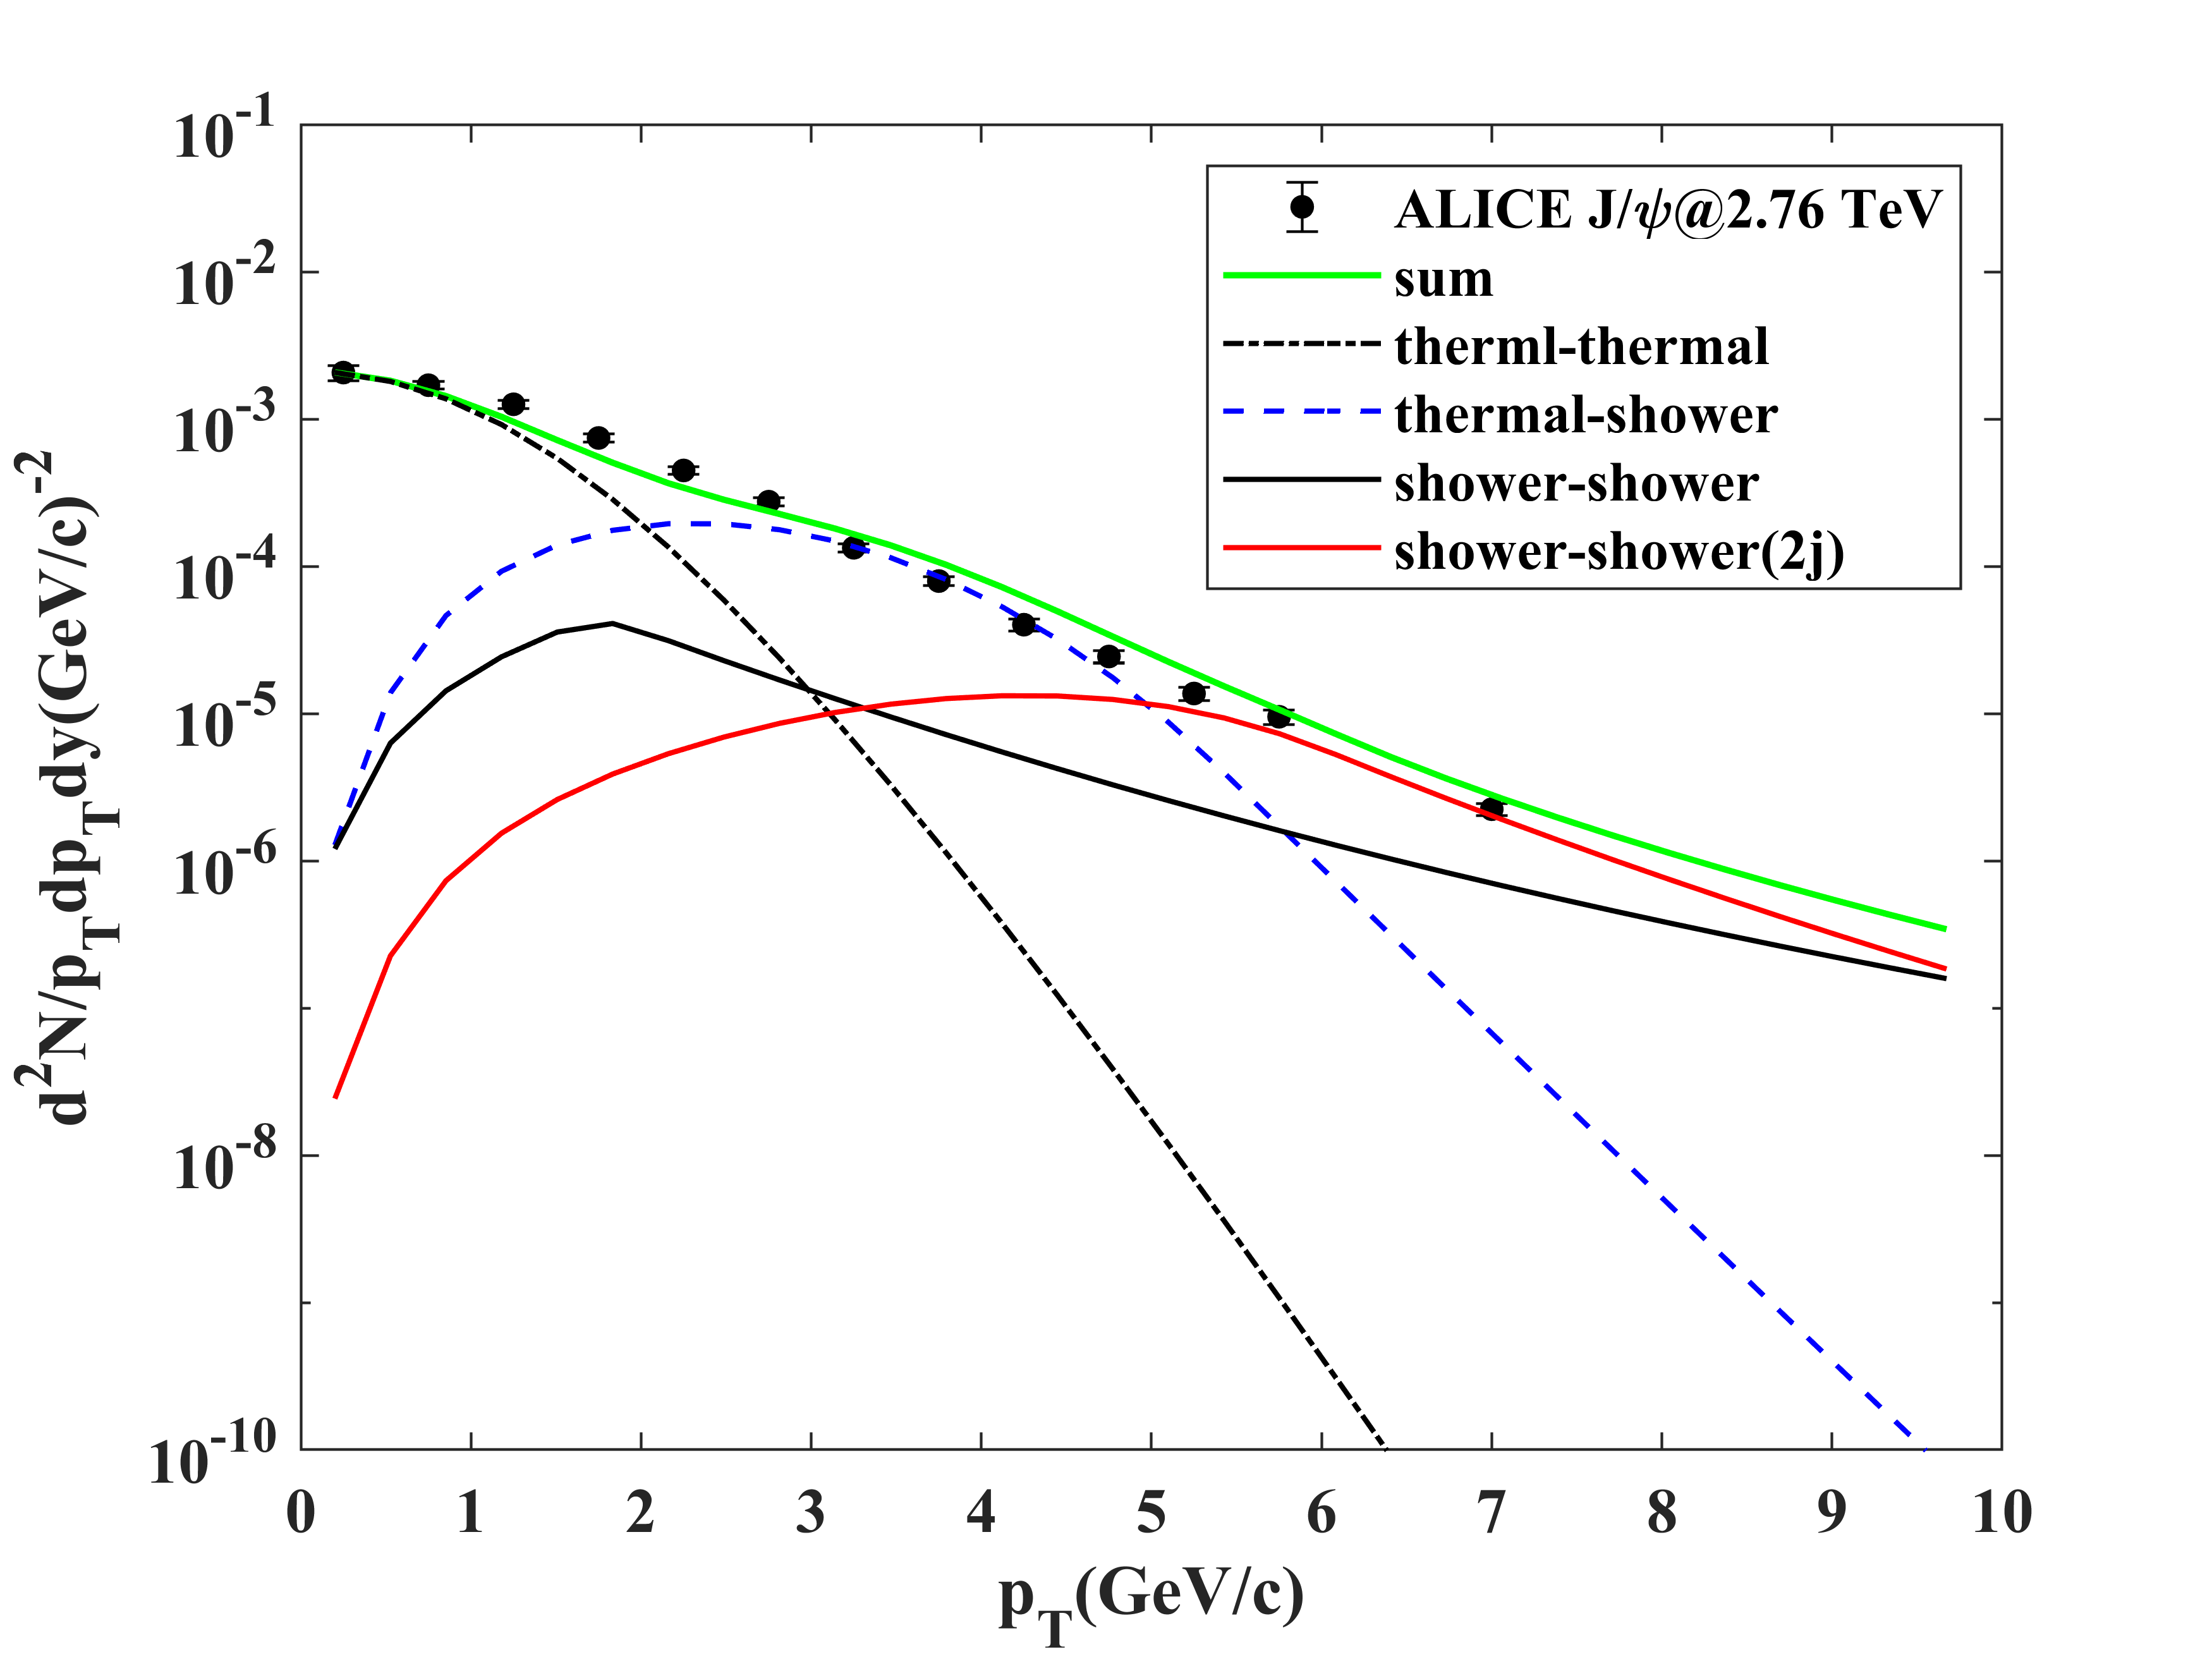
\includegraphics[width=0.45\textwidth]{Jpsi_221031.png}
\caption{$J/\psi$ distribution at 2.76 TeV at 2022/10/31 meeting.}
\label{fig18}
\end{figure}

\subsection{The issue for limit of integral in SS(2j)}\label{integral issue}
The contribution of $SS(2j)$ in mediate $p_T$ region seems too large. Therefore, we would like to do some tests for the limit of integral. Note that
\begin{eqnarray}
	\frac{dN^{SS(2)}_{J/\psi}}{pdp}&=&\frac{10^{-n}}{p^0p}\sum_{\substack{i=g,c\\ i'=g,c}} \int \frac{dq}{q}\frac{dq'}{q'}F'_i(q)F'_{i'}(q')\nonumber \\
	&&\times  S_i^{\overline c}({p\over 2q})   S_{i'}^c({p\over 2q'}), \label{ss2_jpsi}
\end{eqnarray}
First, we set up the integral region in the range of 2 to 30 GeV, and change the lower limit from 2 to $p$ when $p=q$ to insure ${p\over q}<1$. Otherwise when $p>2$ GeV, the lower limit 2 will lead to ${p\over q}>1$.
\begin{eqnarray}
	\frac{dN^{SS(2)}_{J/\psi}}{pdp}&=&\frac{10^{-n}}{p^0p}
	\int^{30}_{2}\int^{30}_{2}
	\sum_{\substack{i=g,c\\ i'=g,c}}  \frac{dq}{q}\frac{dq'}{q'}F'_i(q)F'_{i'}(q')\nonumber \\
	&&\times  S_i^{\overline c}({p\over 2q})   S_{i'}^c({p\over 2q'})\\
	&&\downarrow   \nonumber \\
	&&\downarrow   \text{when $p>2$}	 \nonumber \\
	&&\downarrow   \nonumber \\
	\frac{dN^{SS(2)}_{J/\psi}}{pdp}&=&\frac{10^{-n}}{p^0p}
	\int^{30}_{p}\int^{30}_{p}
	\sum_{\substack{i=g,c\\ i'=g,c}}  \frac{dq}{q}\frac{dq'}{q'}F'_i(q)F'_{i'}(q')\nonumber \\
	&&\times  S_i^{\overline c}({p\over 2q})   S_{i'}^c({p\over 2q'}) 
\end{eqnarray}
The results are shown in Fig.\ref{fig19}.
\begin{figure}[H]
	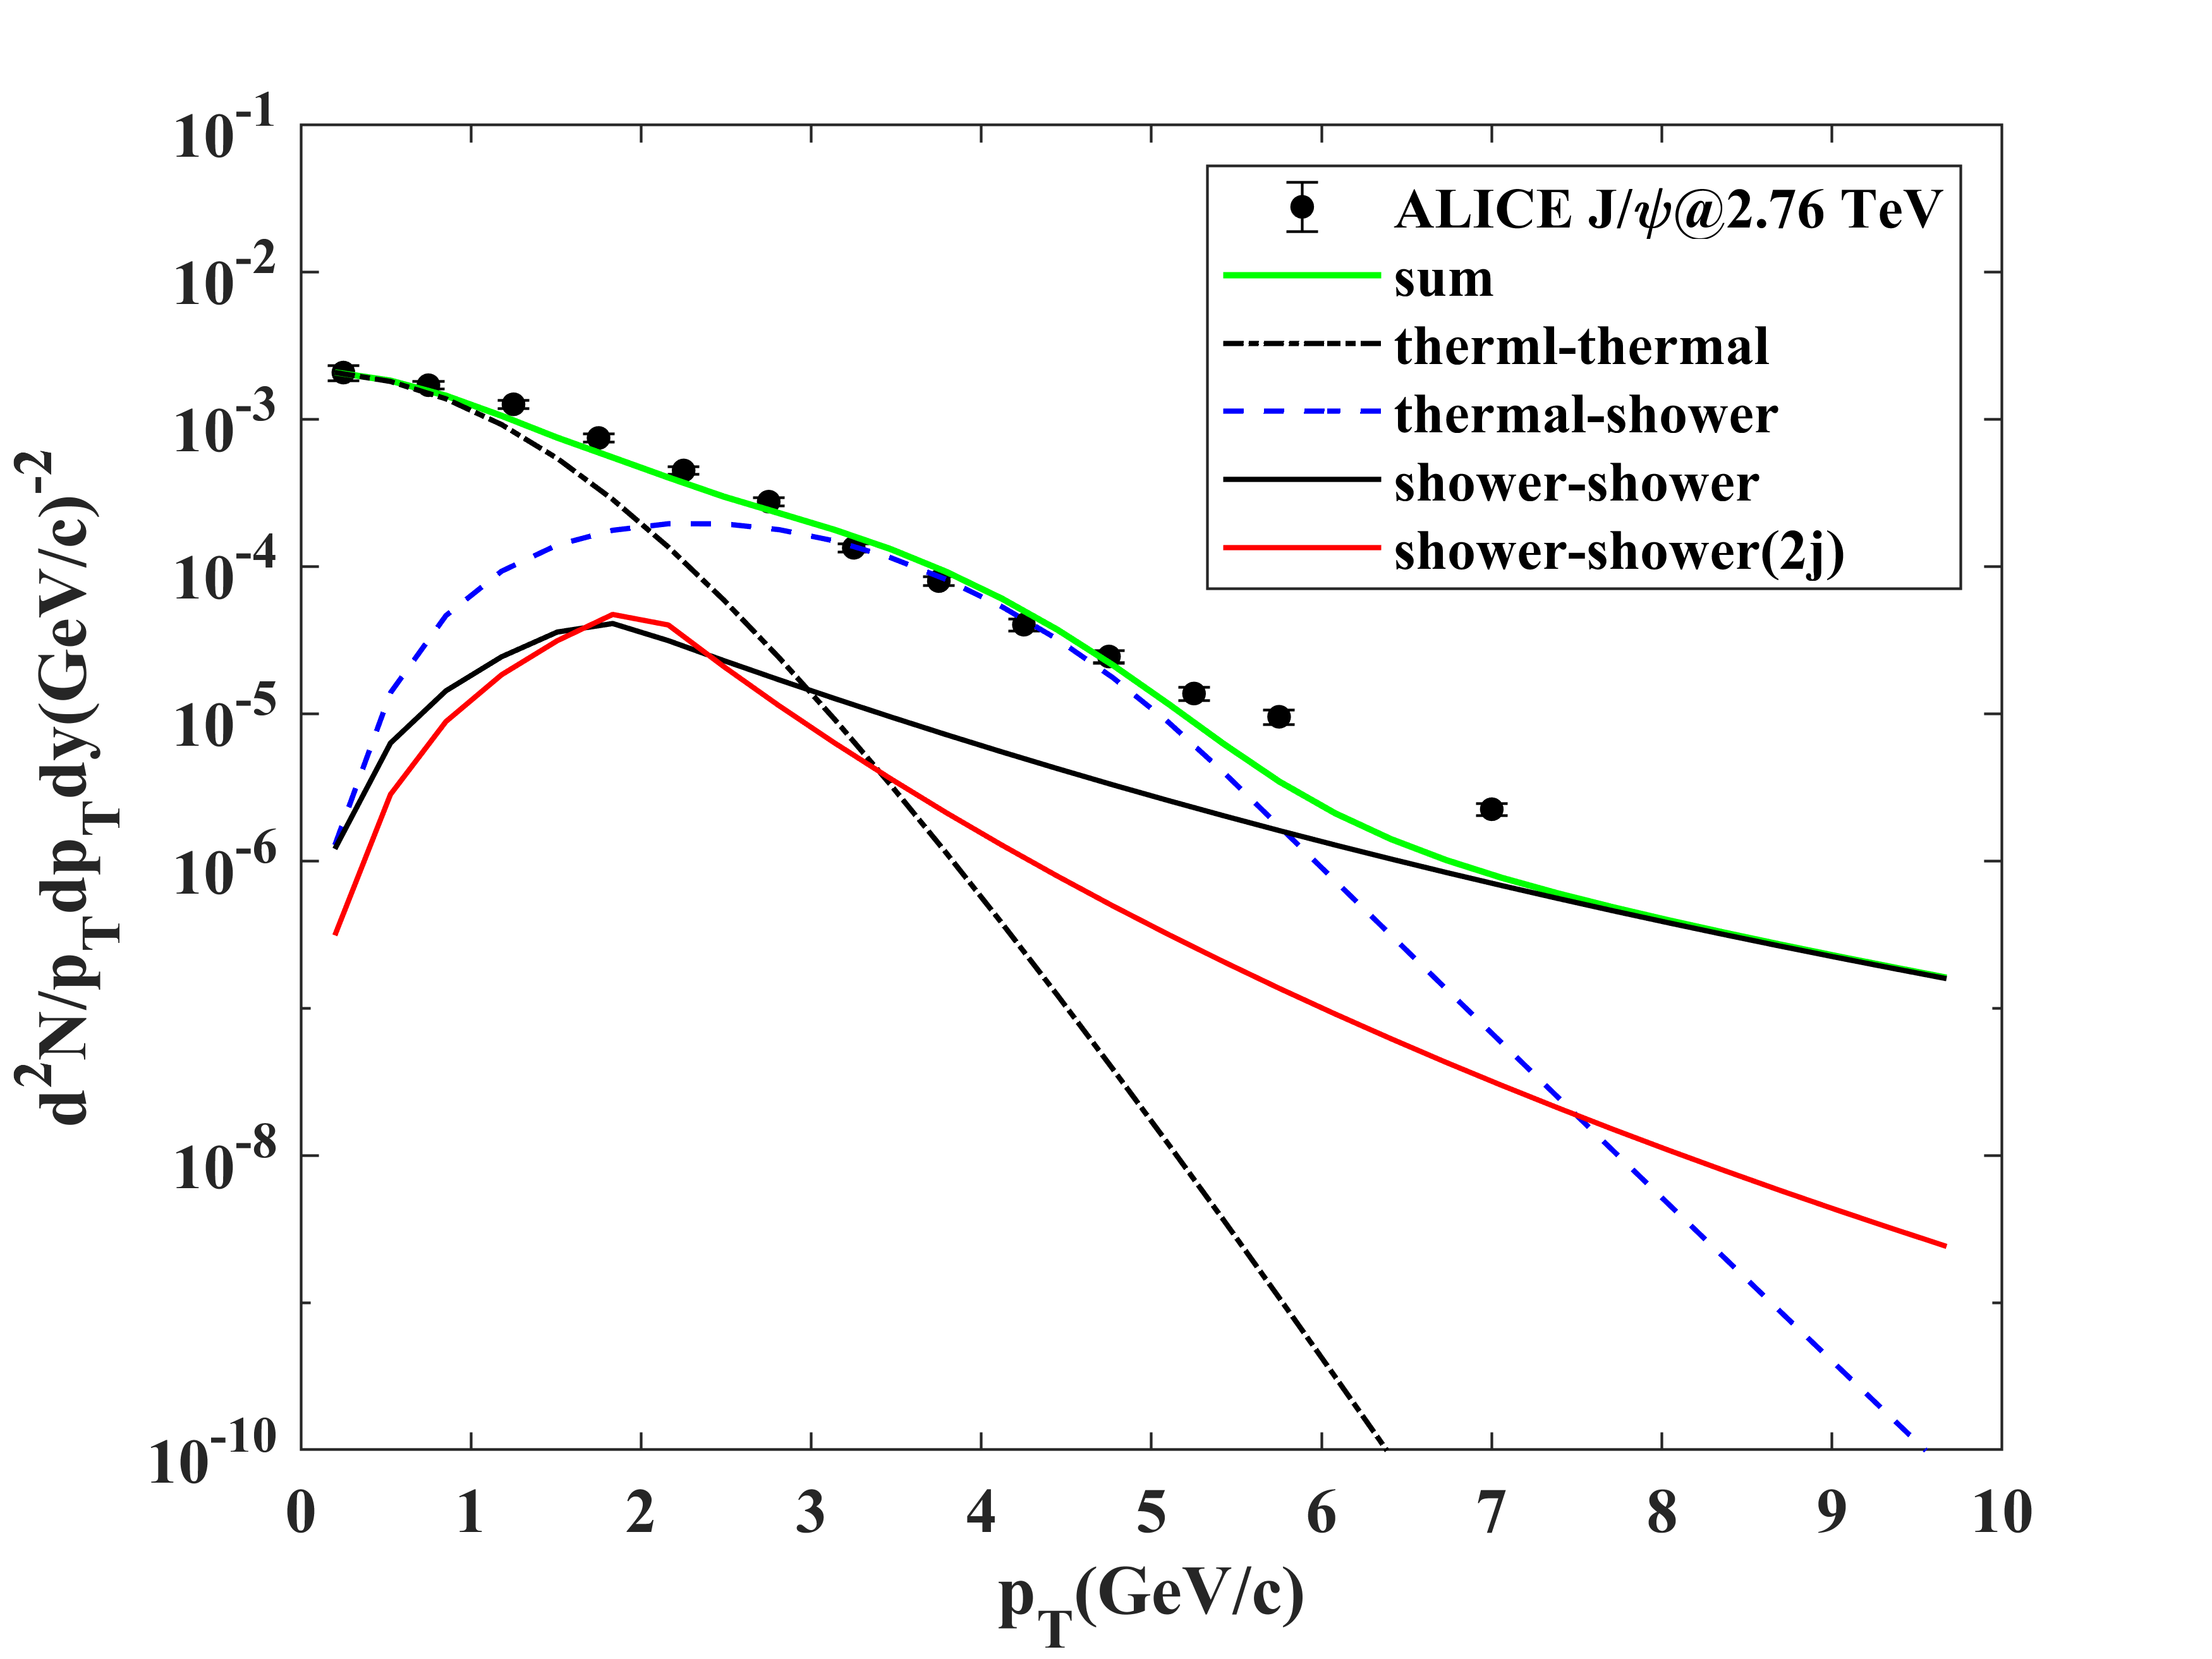
\includegraphics[width=0.45\textwidth]{p_2_30.png}
	\caption{$J/\psi$ distribution at 2.76 TeV. $SS(2j)$: from 2 to 30 and from $p$ to 30 when $p>2$.}
	\label{fig19}
\end{figure}

Then we change the lower limit from 2 to $p/2$ when $p/2=q$ to insure ${p\over 2q}<1$.
\begin{eqnarray}
	\frac{dN^{SS(2)}_{J/\psi}}{pdp}&=&\frac{10^{-n}}{p^0p}
	\int^{30}_{2}\int^{30}_{2}
	\sum_{\substack{i=g,c\\ i'=g,c}}  \frac{dq}{q}\frac{dq'}{q'}F'_i(q)F'_{i'}(q')\nonumber \\
	&&\times  S_i^{\overline c}({p\over 2q})   S_{i'}^c({p\over 2q'})\\
	&&\downarrow   \nonumber \\
	&&\downarrow   \text{when $p>4$}	 \nonumber \\
	&&\downarrow   \nonumber \\
	\frac{dN^{SS(2)}_{J/\psi}}{pdp}&=&\frac{10^{-n}}{p^0p}
	\int^{30}_{p/2}\int^{30}_{p/2}
	\sum_{\substack{i=g,c\\ i'=g,c}}  \frac{dq}{q}\frac{dq'}{q'}F'_i(q)F'_{i'}(q')\nonumber \\
	&&\times  S_i^{\overline c}({p\over 2q})   S_{i'}^c({p\over 2q'})\label{int_ss2j}
\end{eqnarray}
The results are shown in Fig.\ref{fig20}.
\begin{figure}[H]
	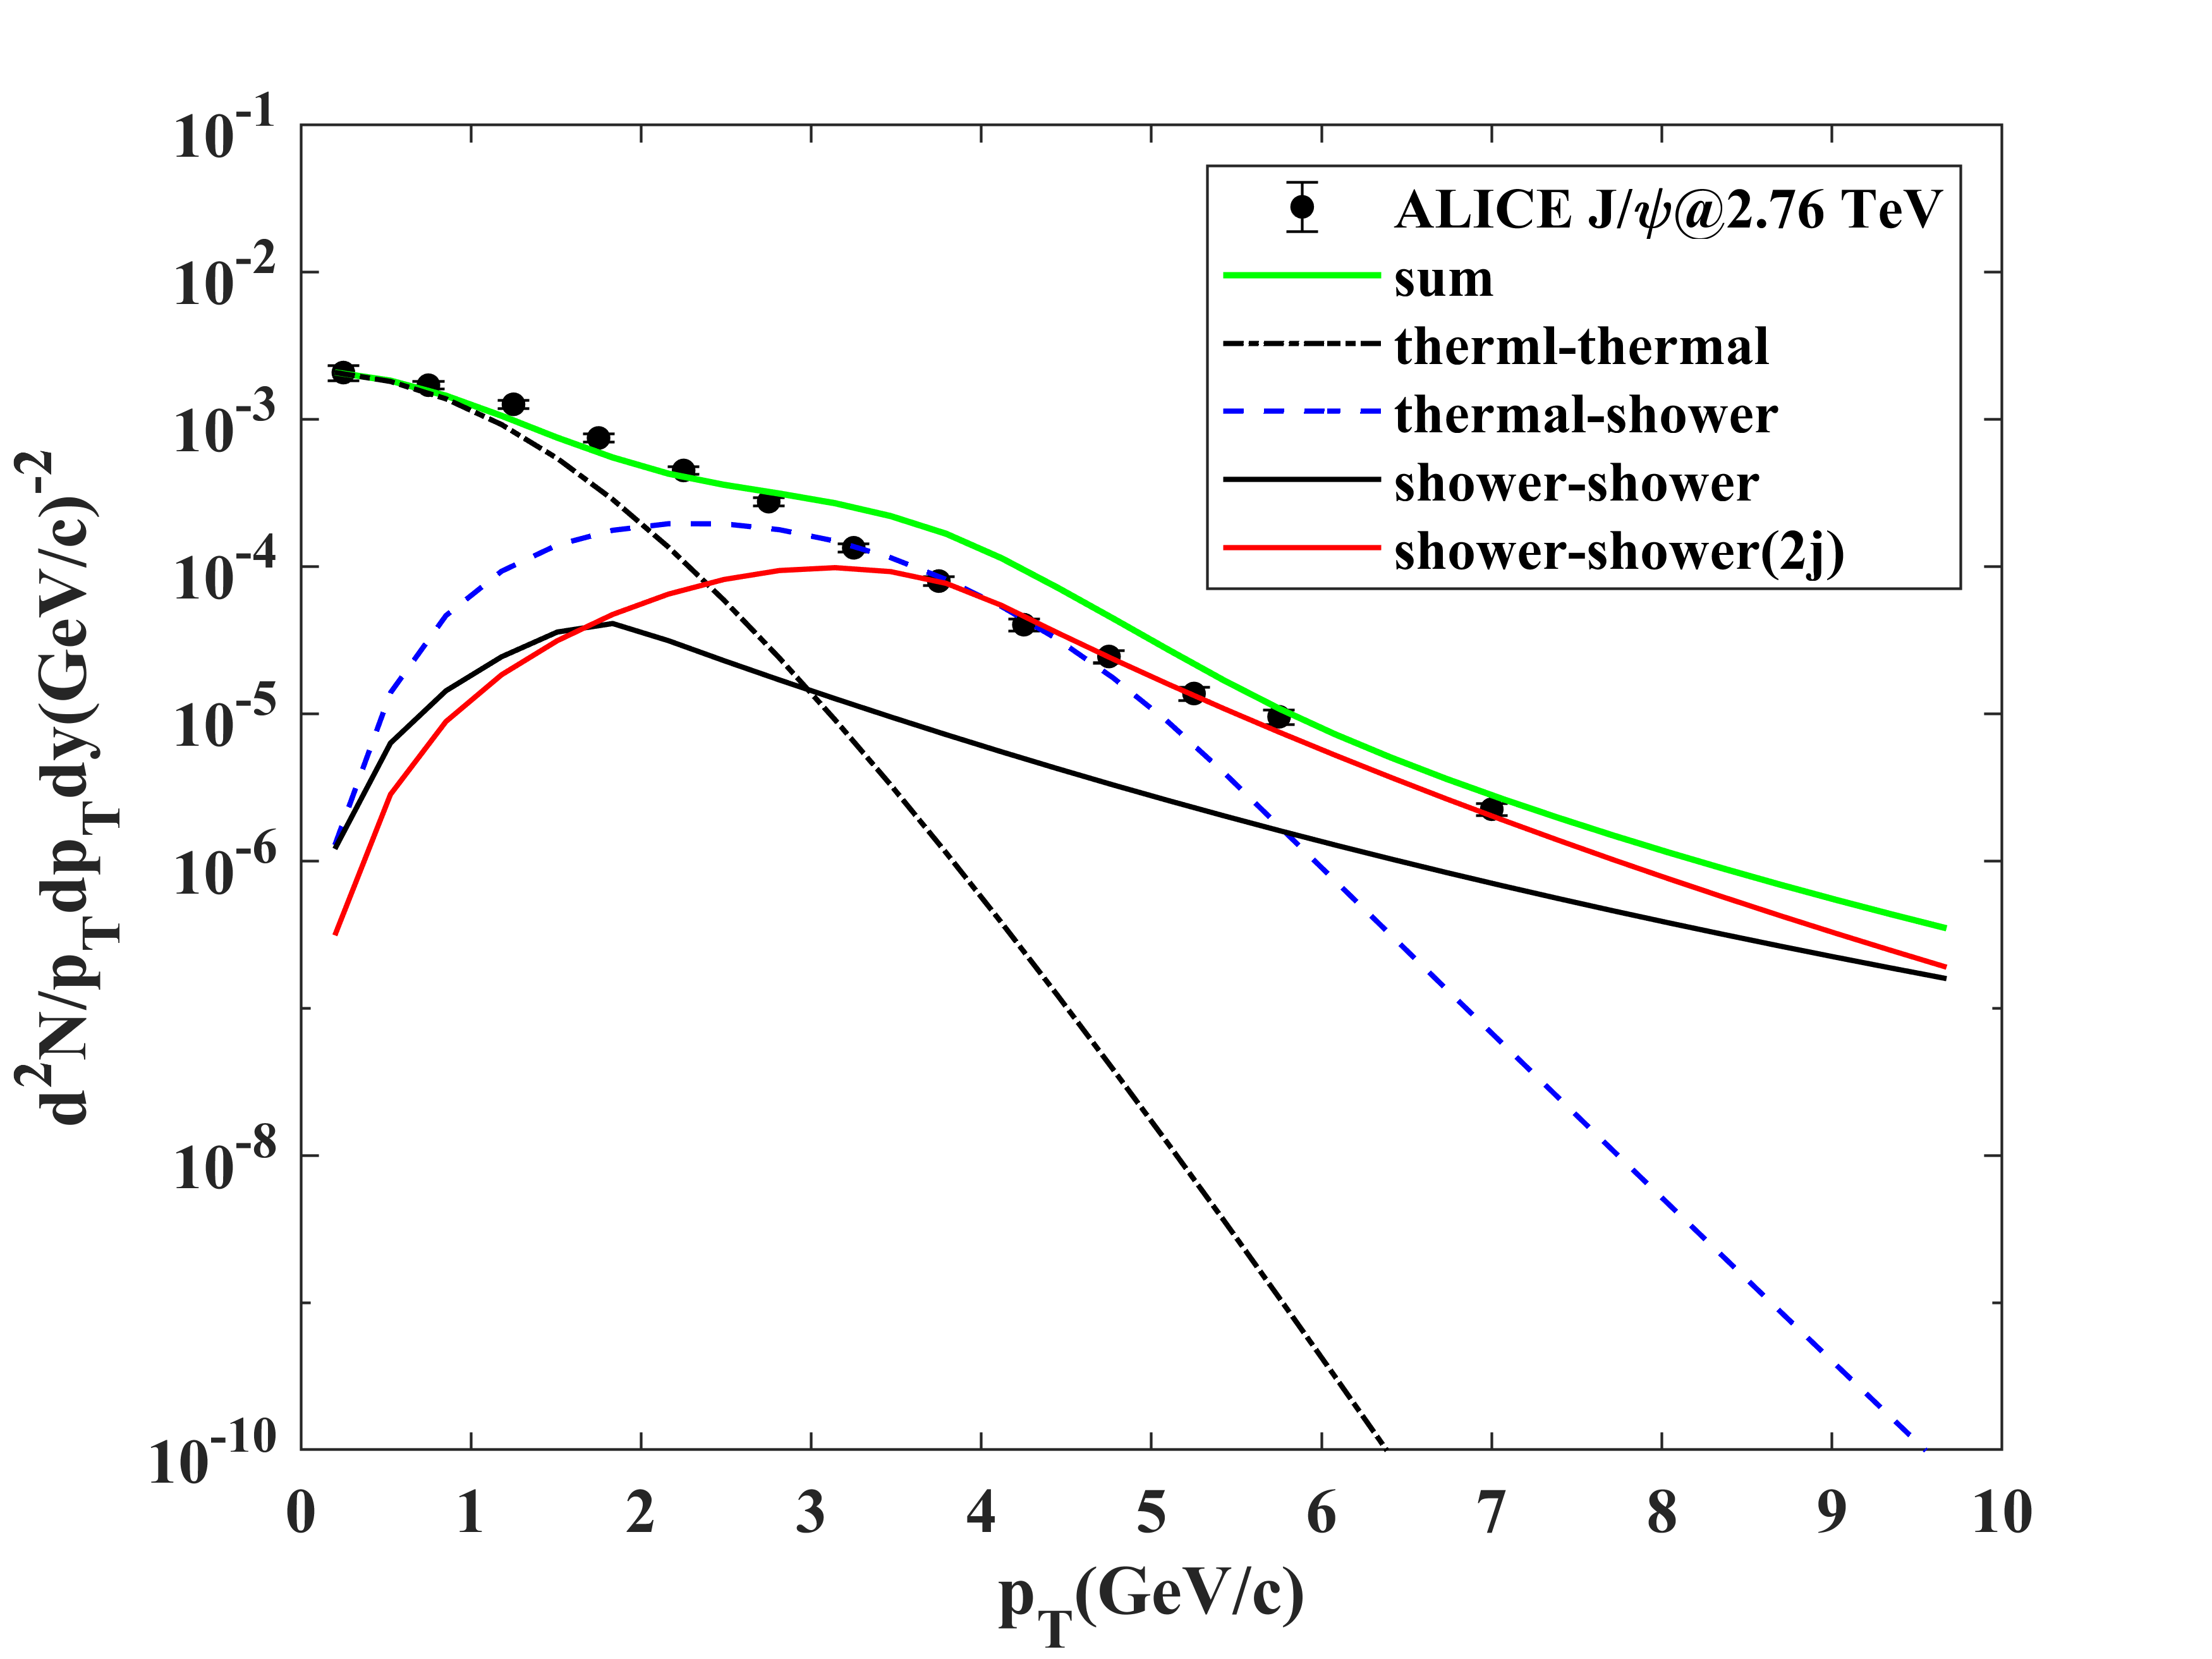
\includegraphics[width=0.45\textwidth]{2p_2_30.png}
	\caption{$J/\psi$ distribution at 2.76 TeV. $SS(2j)$: from 2 to 30 and from $p/2$ to 30 when $p>4$.}
	\label{fig20}
\end{figure}

To fit the data, we change the initial lower limit of integral from 2 to 3 and everything else remains the same.
\begin{eqnarray}
	\frac{dN^{SS(2)}_{J/\psi}}{pdp}&=&\frac{10^{-n}}{p^0p}
	\int^{30}_{3}\int^{30}_{3}
	\sum_{\substack{i=g,c\\ i'=g,c}}  \frac{dq}{q}\frac{dq'}{q'}F'_i(q)F'_{i'}(q')\nonumber \\
	&&\times  S_i^{\overline c}({p\over 2q})   S_{i'}^c({p\over 2q'})\\
	&&\downarrow   \nonumber \\
	&&\downarrow   \text{when $p>3$}	 \nonumber \\
	&&\downarrow   \nonumber \\
	\frac{dN^{SS(2)}_{J/\psi}}{pdp}&=&\frac{10^{-n}}{p^0p}
	\int^{30}_{p}\int^{30}_{p}
	\sum_{\substack{i=g,c\\ i'=g,c}}  \frac{dq}{q}\frac{dq'}{q'}F'_i(q)F'_{i'}(q')\nonumber \\
	&&\times  S_i^{\overline c}({p\over 2q})   S_{i'}^c({p\over 2q'})
\end{eqnarray}
The results are shown in Fig.\ref{fig21}.
\begin{figure}[H]
	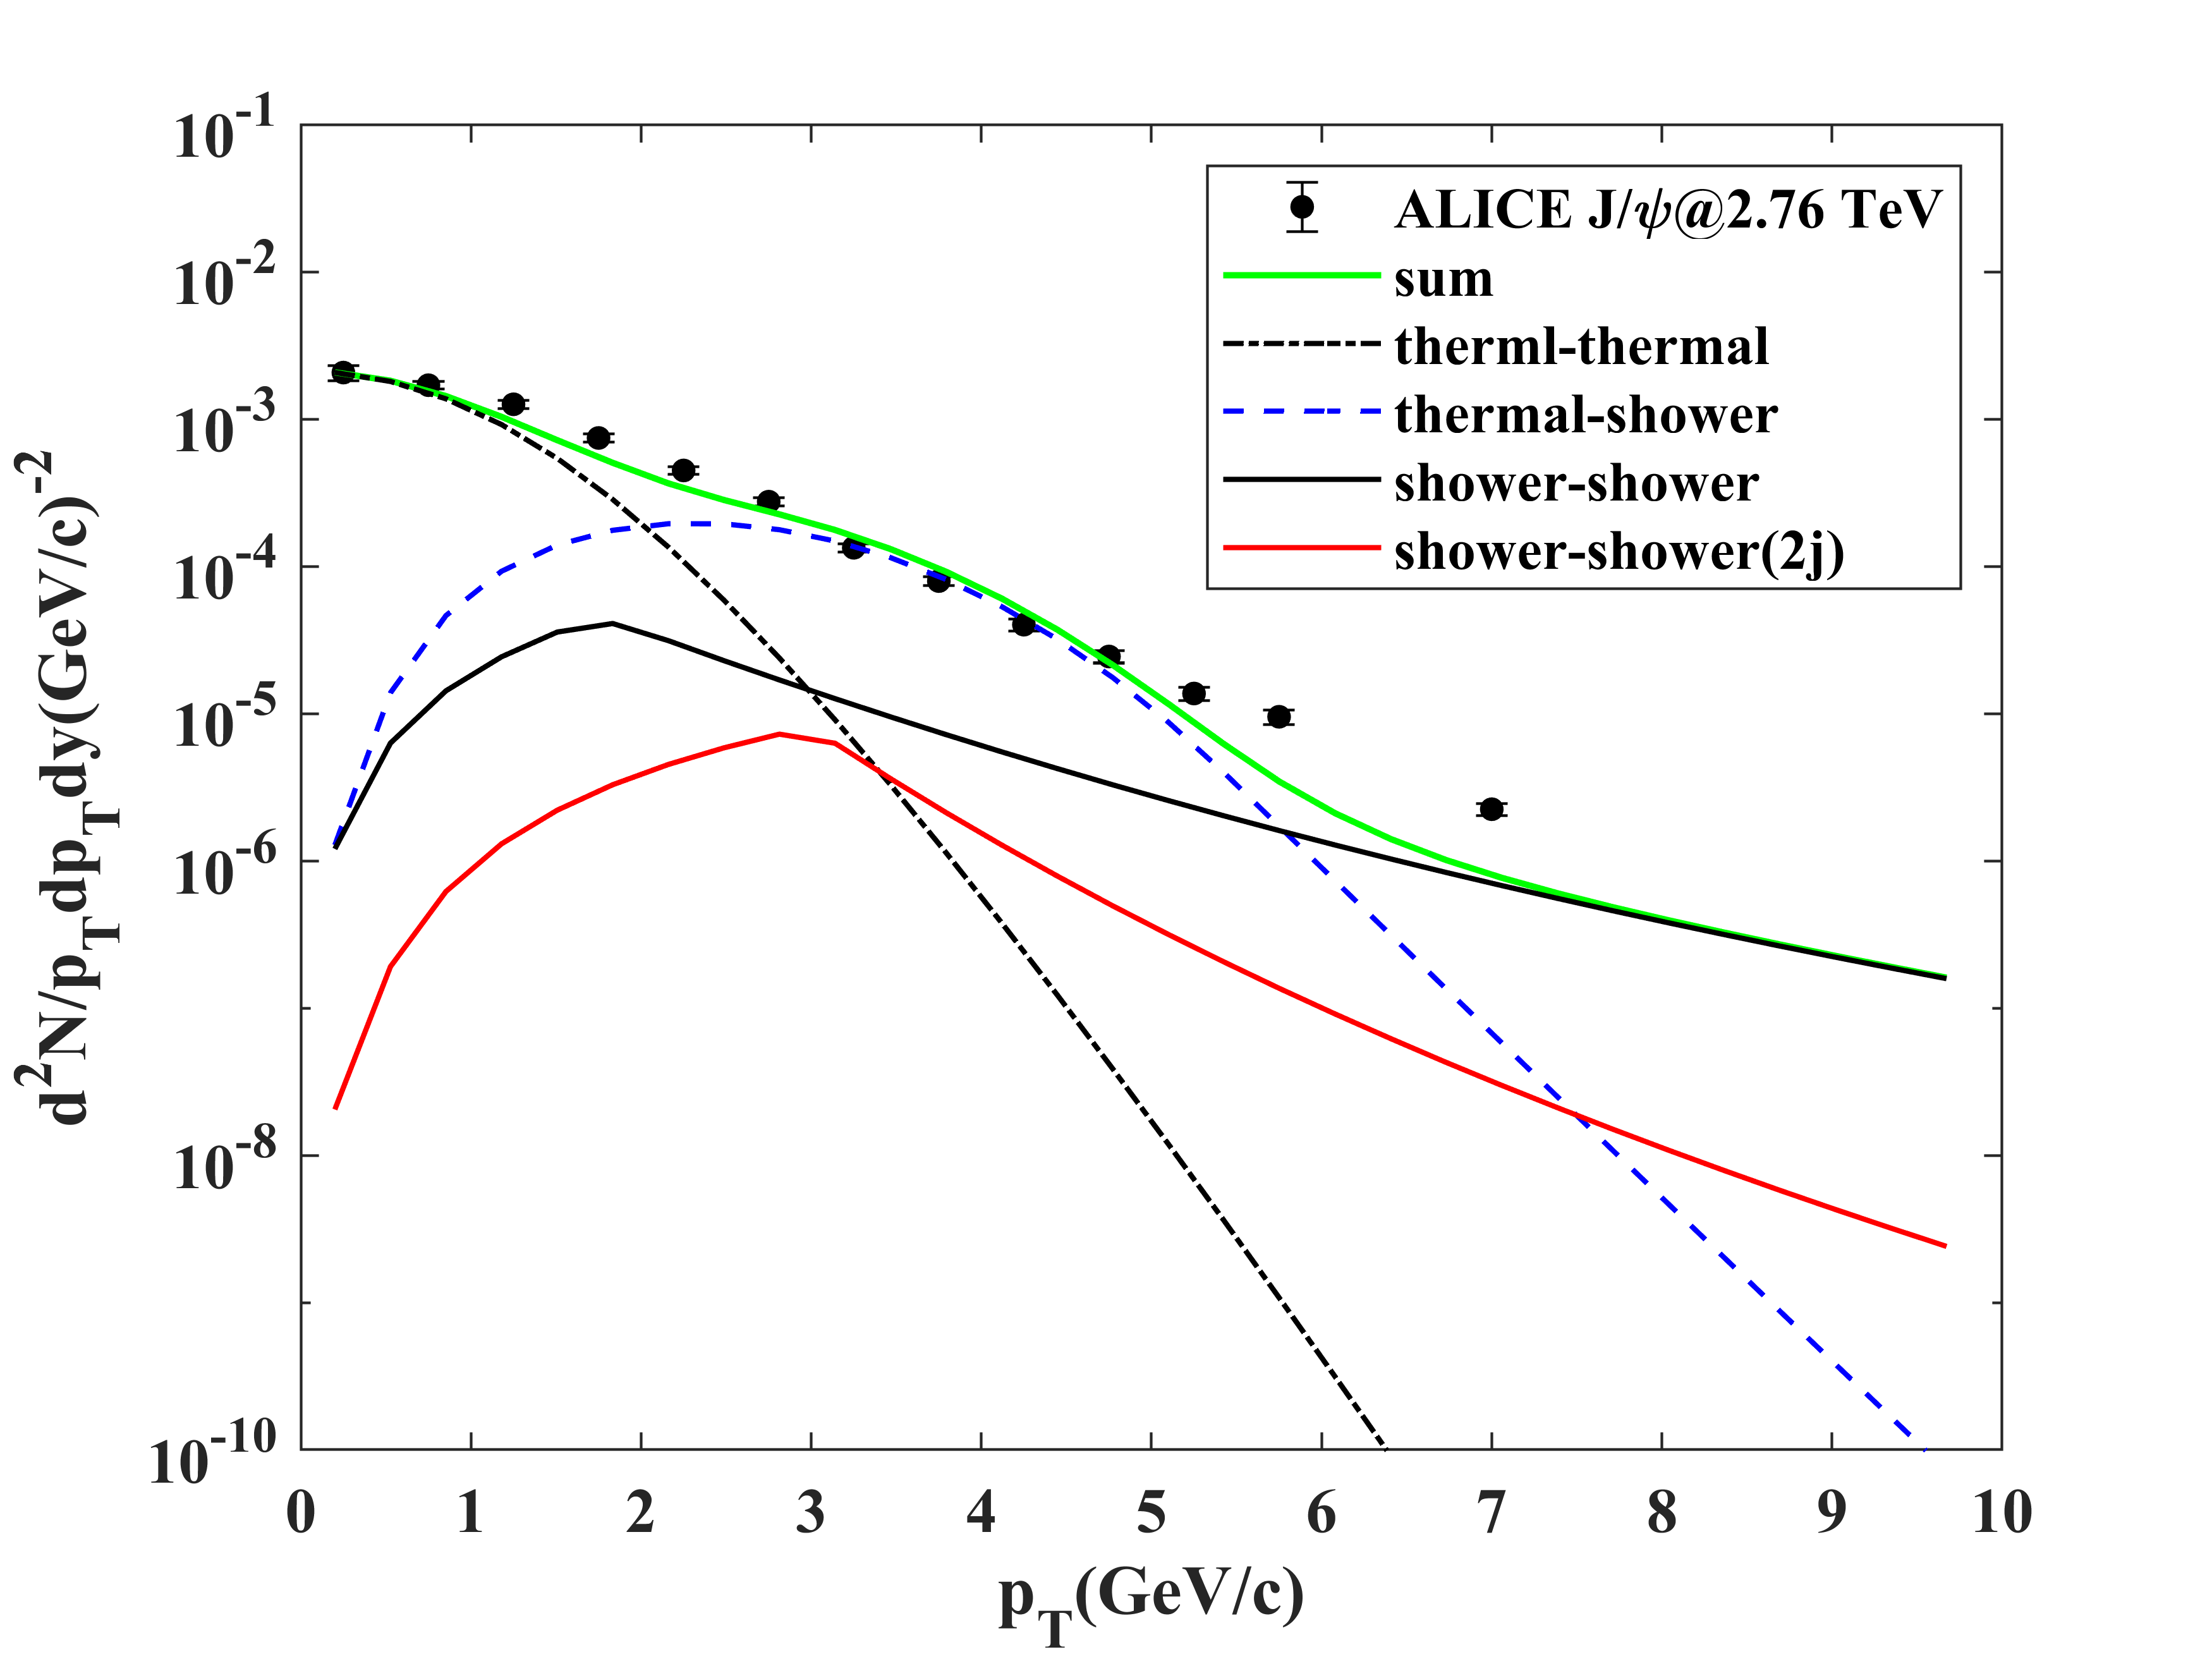
\includegraphics[width=0.45\textwidth]{p_3_30.png}
	\caption{$J/\psi$ distribution at 2.76 TeV. $SS(2j)$: from 3 to 30 and from $p$ to 30 when $p>2$.}
	\label{fig21}
\end{figure}

Then we change the lower limit from 3 to $p/2$ when $p/2=q$ to insure ${p\over 2q}<1$.
\begin{eqnarray}
	\frac{dN^{SS(2)}_{J/\psi}}{pdp}&=&\frac{10^{-n}}{p^0p}
	\int^{30}_{3}\int^{30}_{3}
	\sum_{\substack{i=g,c\\ i'=g,c}}  \frac{dq}{q}\frac{dq'}{q'}F'_i(q)F'_{i'}(q')\nonumber \\
	&&\times  S_i^{\overline c}({p\over 2q})   S_{i'}^c({p\over 2q'})\\
	&&\downarrow   \nonumber \\
	&&\downarrow   \text{when $p>6$}	 \nonumber \\
	&&\downarrow   \nonumber \\
	\frac{dN^{SS(2)}_{J/\psi}}{pdp}&=&\frac{10^{-n}}{p^0p}
	\int^{30}_{p/2}\int^{30}_{p/2}
	\sum_{\substack{i=g,c\\ i'=g,c}}  \frac{dq}{q}\frac{dq'}{q'}F'_i(q)F'_{i'}(q')\nonumber \\
	&&\times  S_i^{\overline c}({p\over 2q})   S_{i'}^c({p\over 2q'})
\end{eqnarray}
The results are shown in Fig.\ref{fig22}.
\begin{figure}[H]
	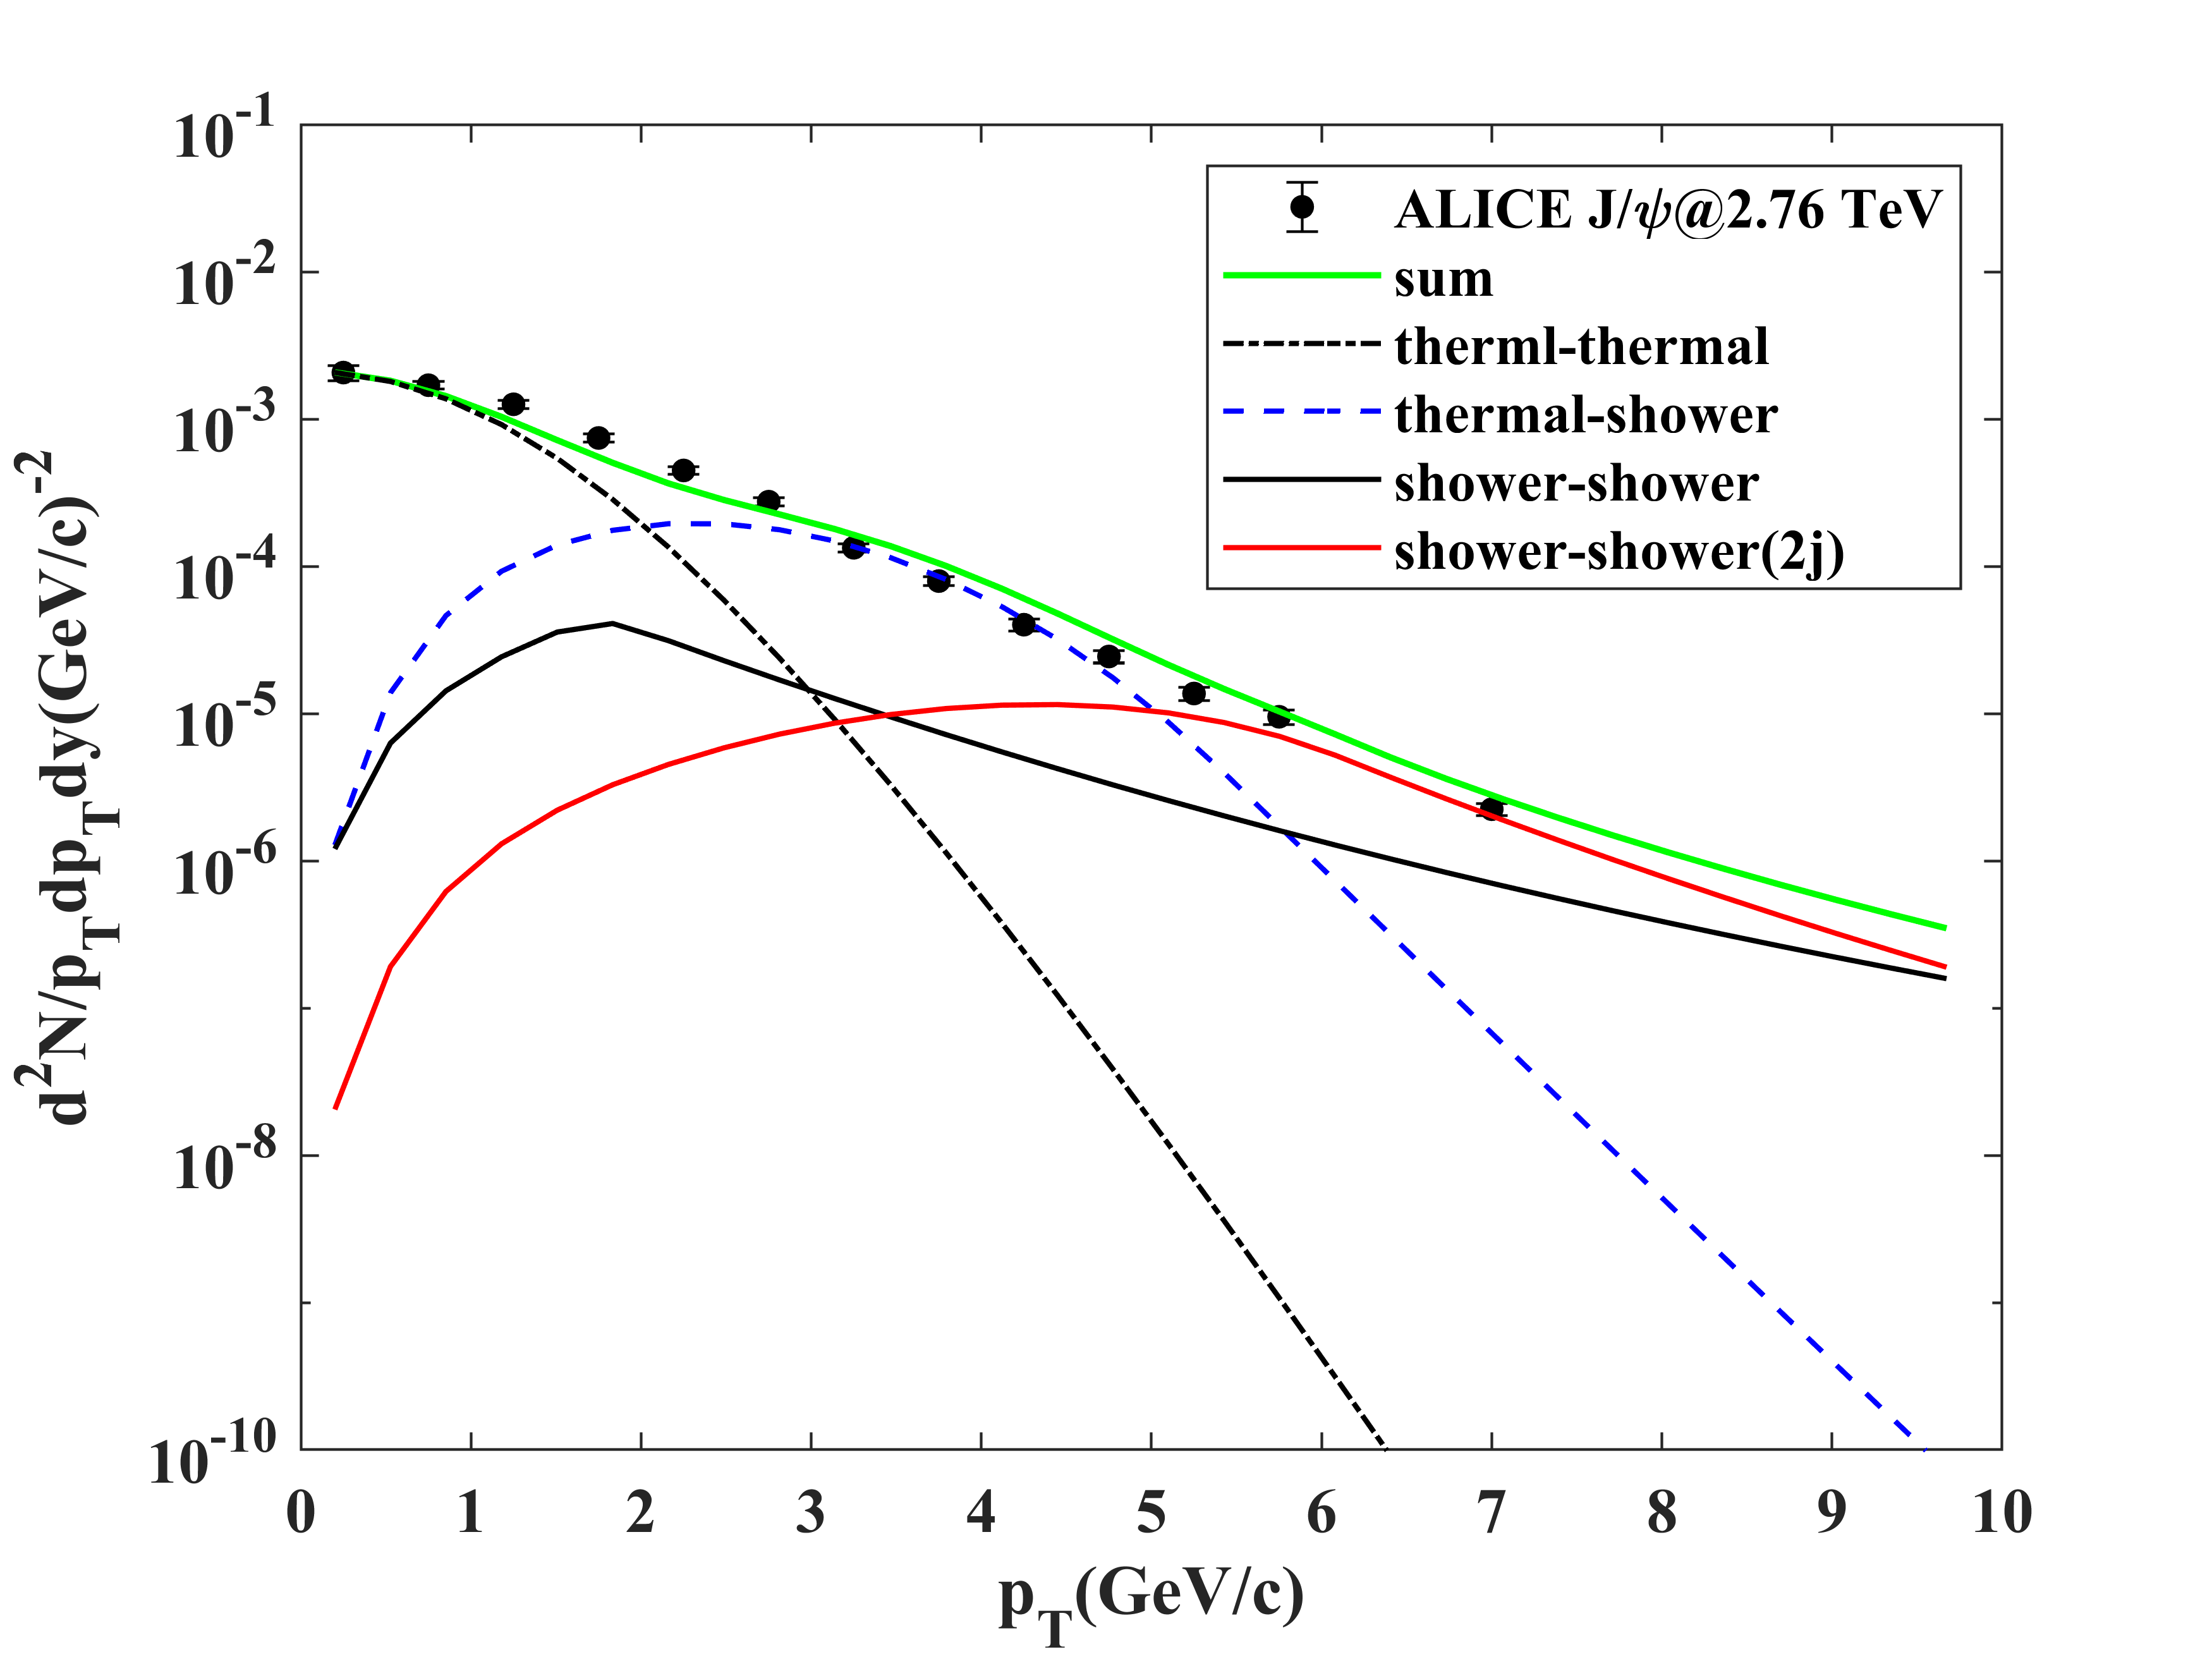
\includegraphics[width=0.45\textwidth]{2p_3_30.png}
	\caption{$J/\psi$ distribution at 2.76 TeV. $SS(2j)$: from 3 to 30 and from $p/2$ to 30 when $p>6$.}
	\label{fig22}
\end{figure}
All are listed above with $\Gamma=10^{-2}$. 

\section{Meeting 2022.11.07}
We try to fit the distributions of charmed mesons with improved approaches above. The best results by fitting are shown in this section.
And all the parameters used are listed here:
\begin{eqnarray}
	\text{2.76 TeV}&:&  \nonumber \\
	&&T=0.185 \text{ GeV}, \Gamma=10^{-2}, \nonumber \\
	&&\gamma_l=1.0,  \gamma_s=0.8 ,\gamma_c=0.26\nonumber \\
	J/\psi&:& v_T=0.25c,  \\ \nonumber
	&&\beta L\rightarrow \text{0 for charm, 2.39 for gluon}\\
	D^0&:& v_T=0.43c,  \beta L=\text{5.8 for all}\\
	D_s&:& v_T=0.3c,    \beta L=\text{4.0 for all}.\\
	\text{5.02 TeV}&:&  \nonumber \\
	&&T=0.185 \text{ GeV}, \Gamma=10^{-2}, \nonumber \\
	&&\gamma_l=0.5,  \gamma_s=0.8 ,\gamma_c=0.49\nonumber \\
	J/\psi&:& v_T=0.28c,  \\ \nonumber
	&&\beta L\rightarrow \text{0 for charm, 2.39 for gluon}\\
	D^0&:& v_T=0.51c,  \beta L=\text{5.8 for all}\\
	D_s&:& v_T=0.4c,    \beta L=\text{4.0 for all}.
\end{eqnarray}

\begin{figure}[H]
	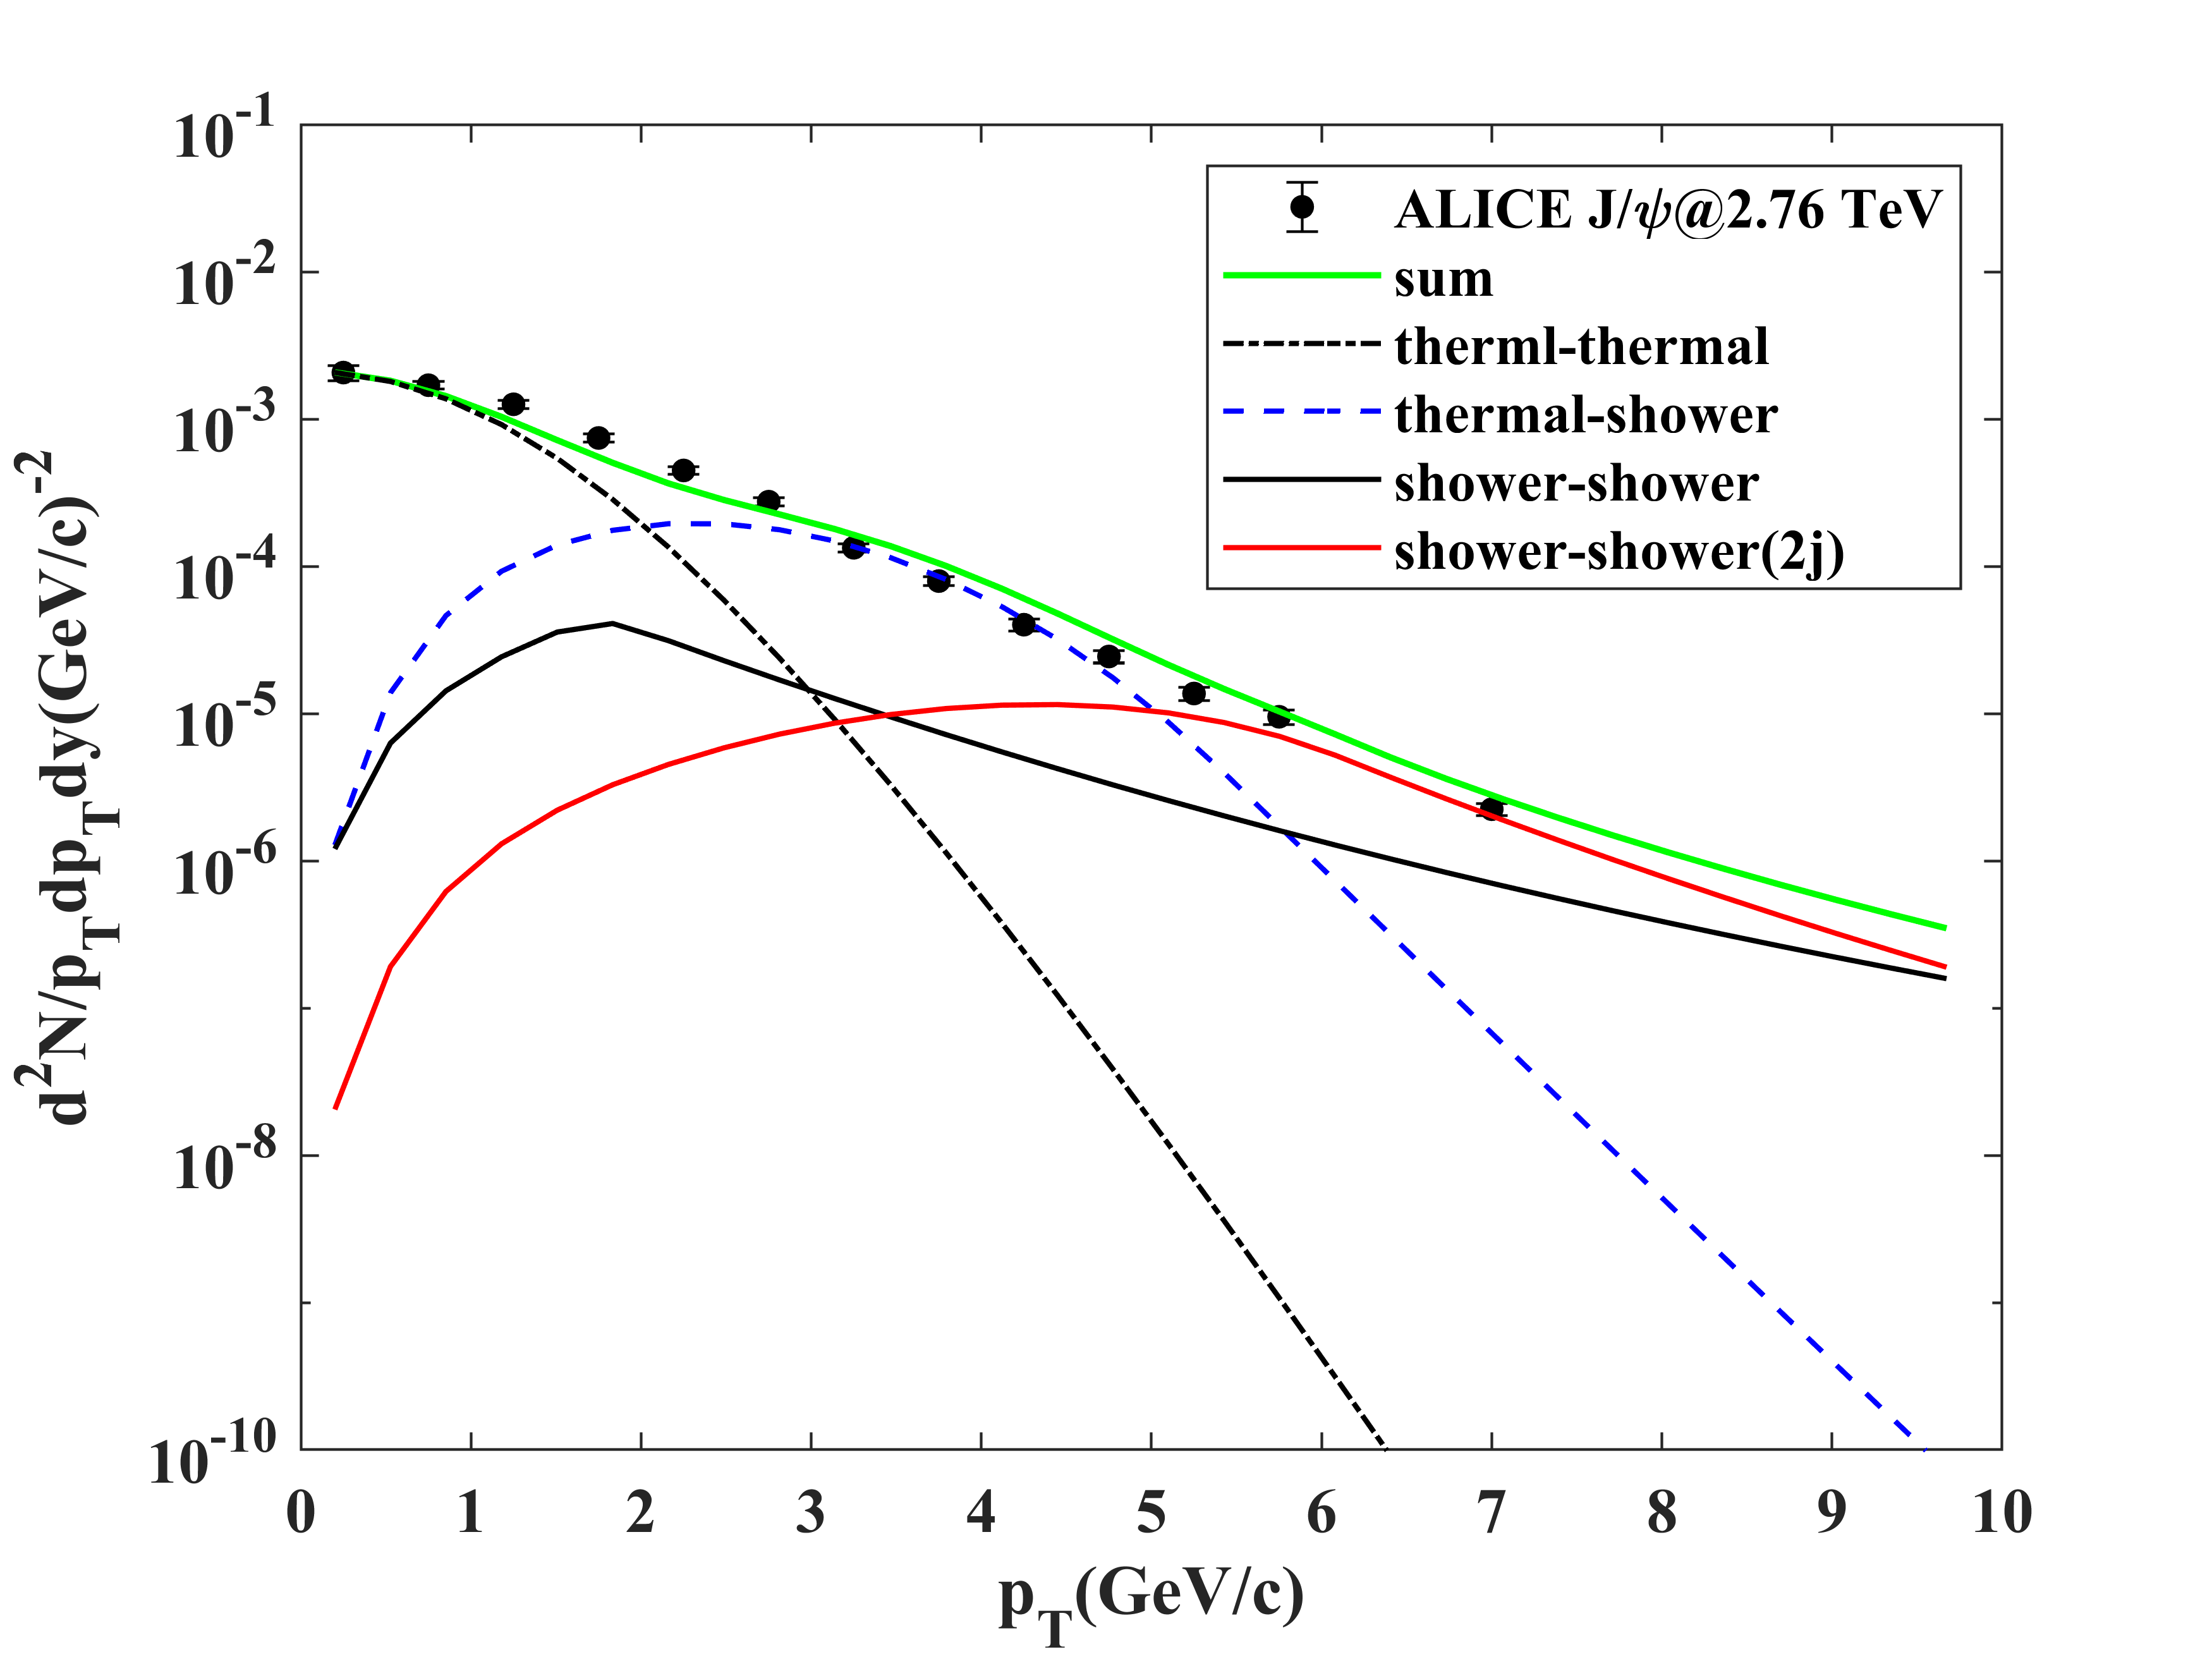
\includegraphics[width=0.45\textwidth]{2p_3_30.png}
	\caption{$J/\psi$ distribution at 2.76 TeV. }
	\label{fig23}
\end{figure}
\begin{figure}[H]
	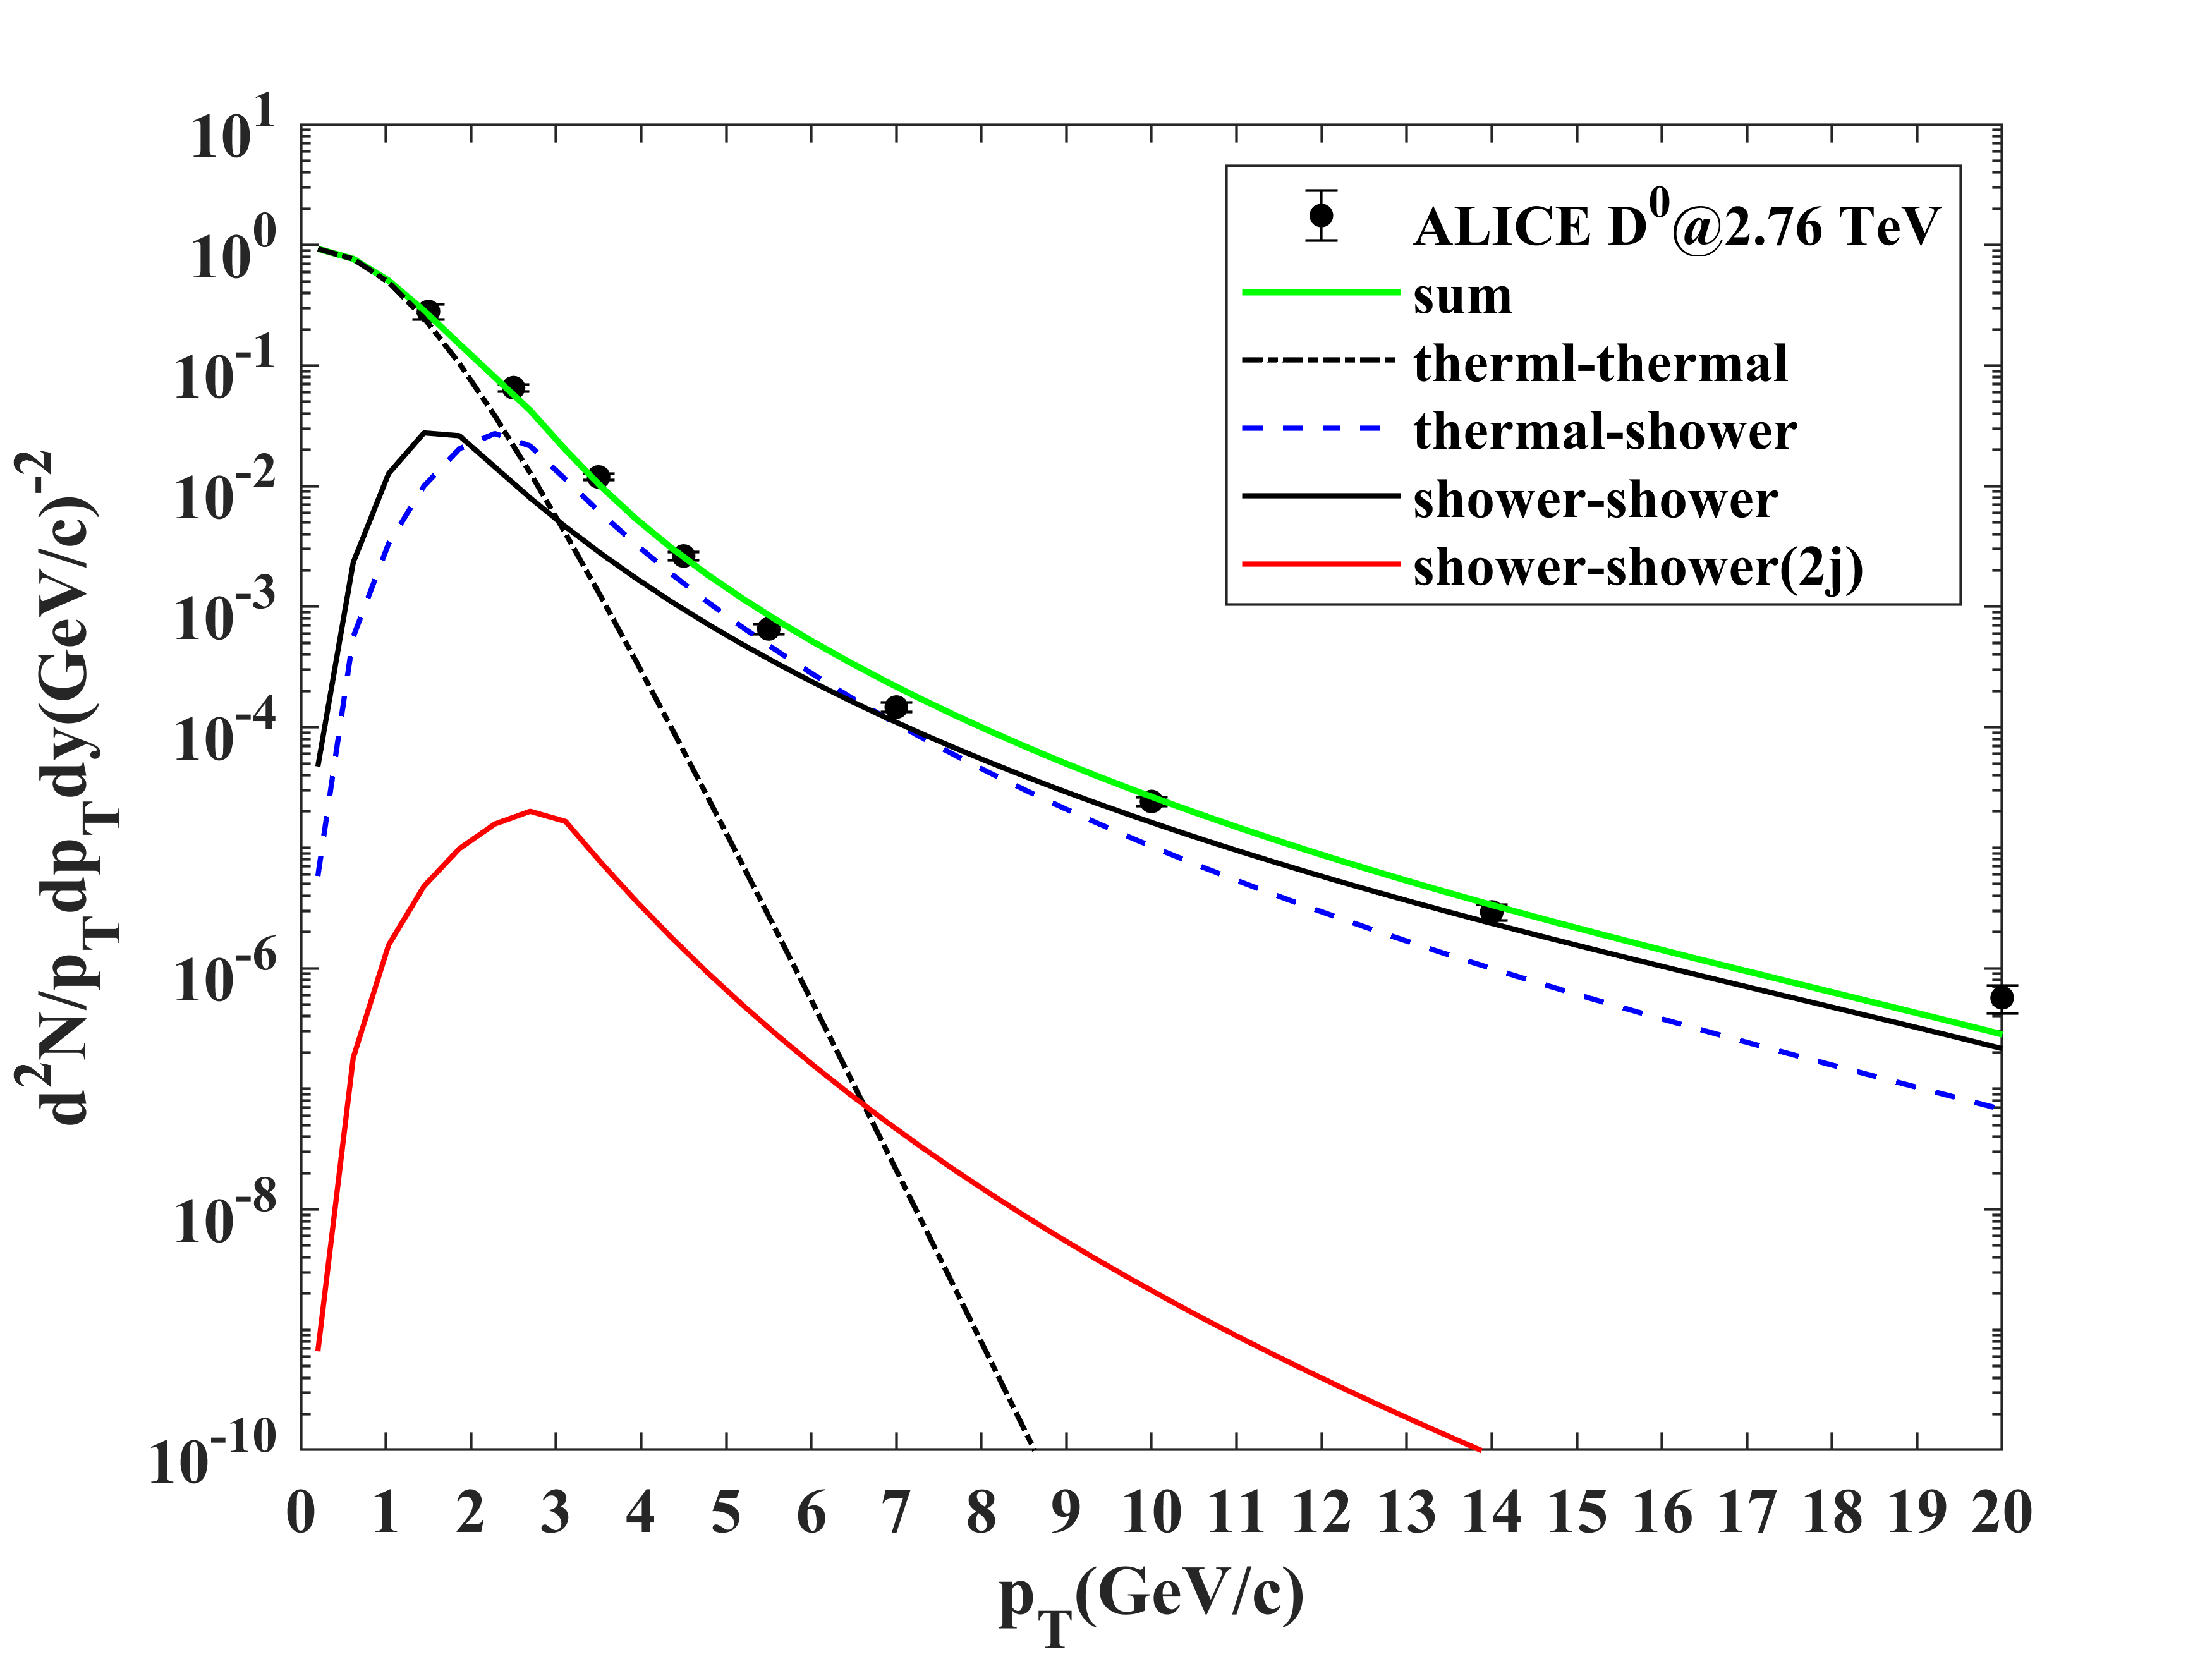
\includegraphics[width=0.45\textwidth]{D0_1106.png}
	\caption{$D^0$ distribution at 2.76 TeV. }
	\label{fig24}
\end{figure}
\begin{figure}[H]
	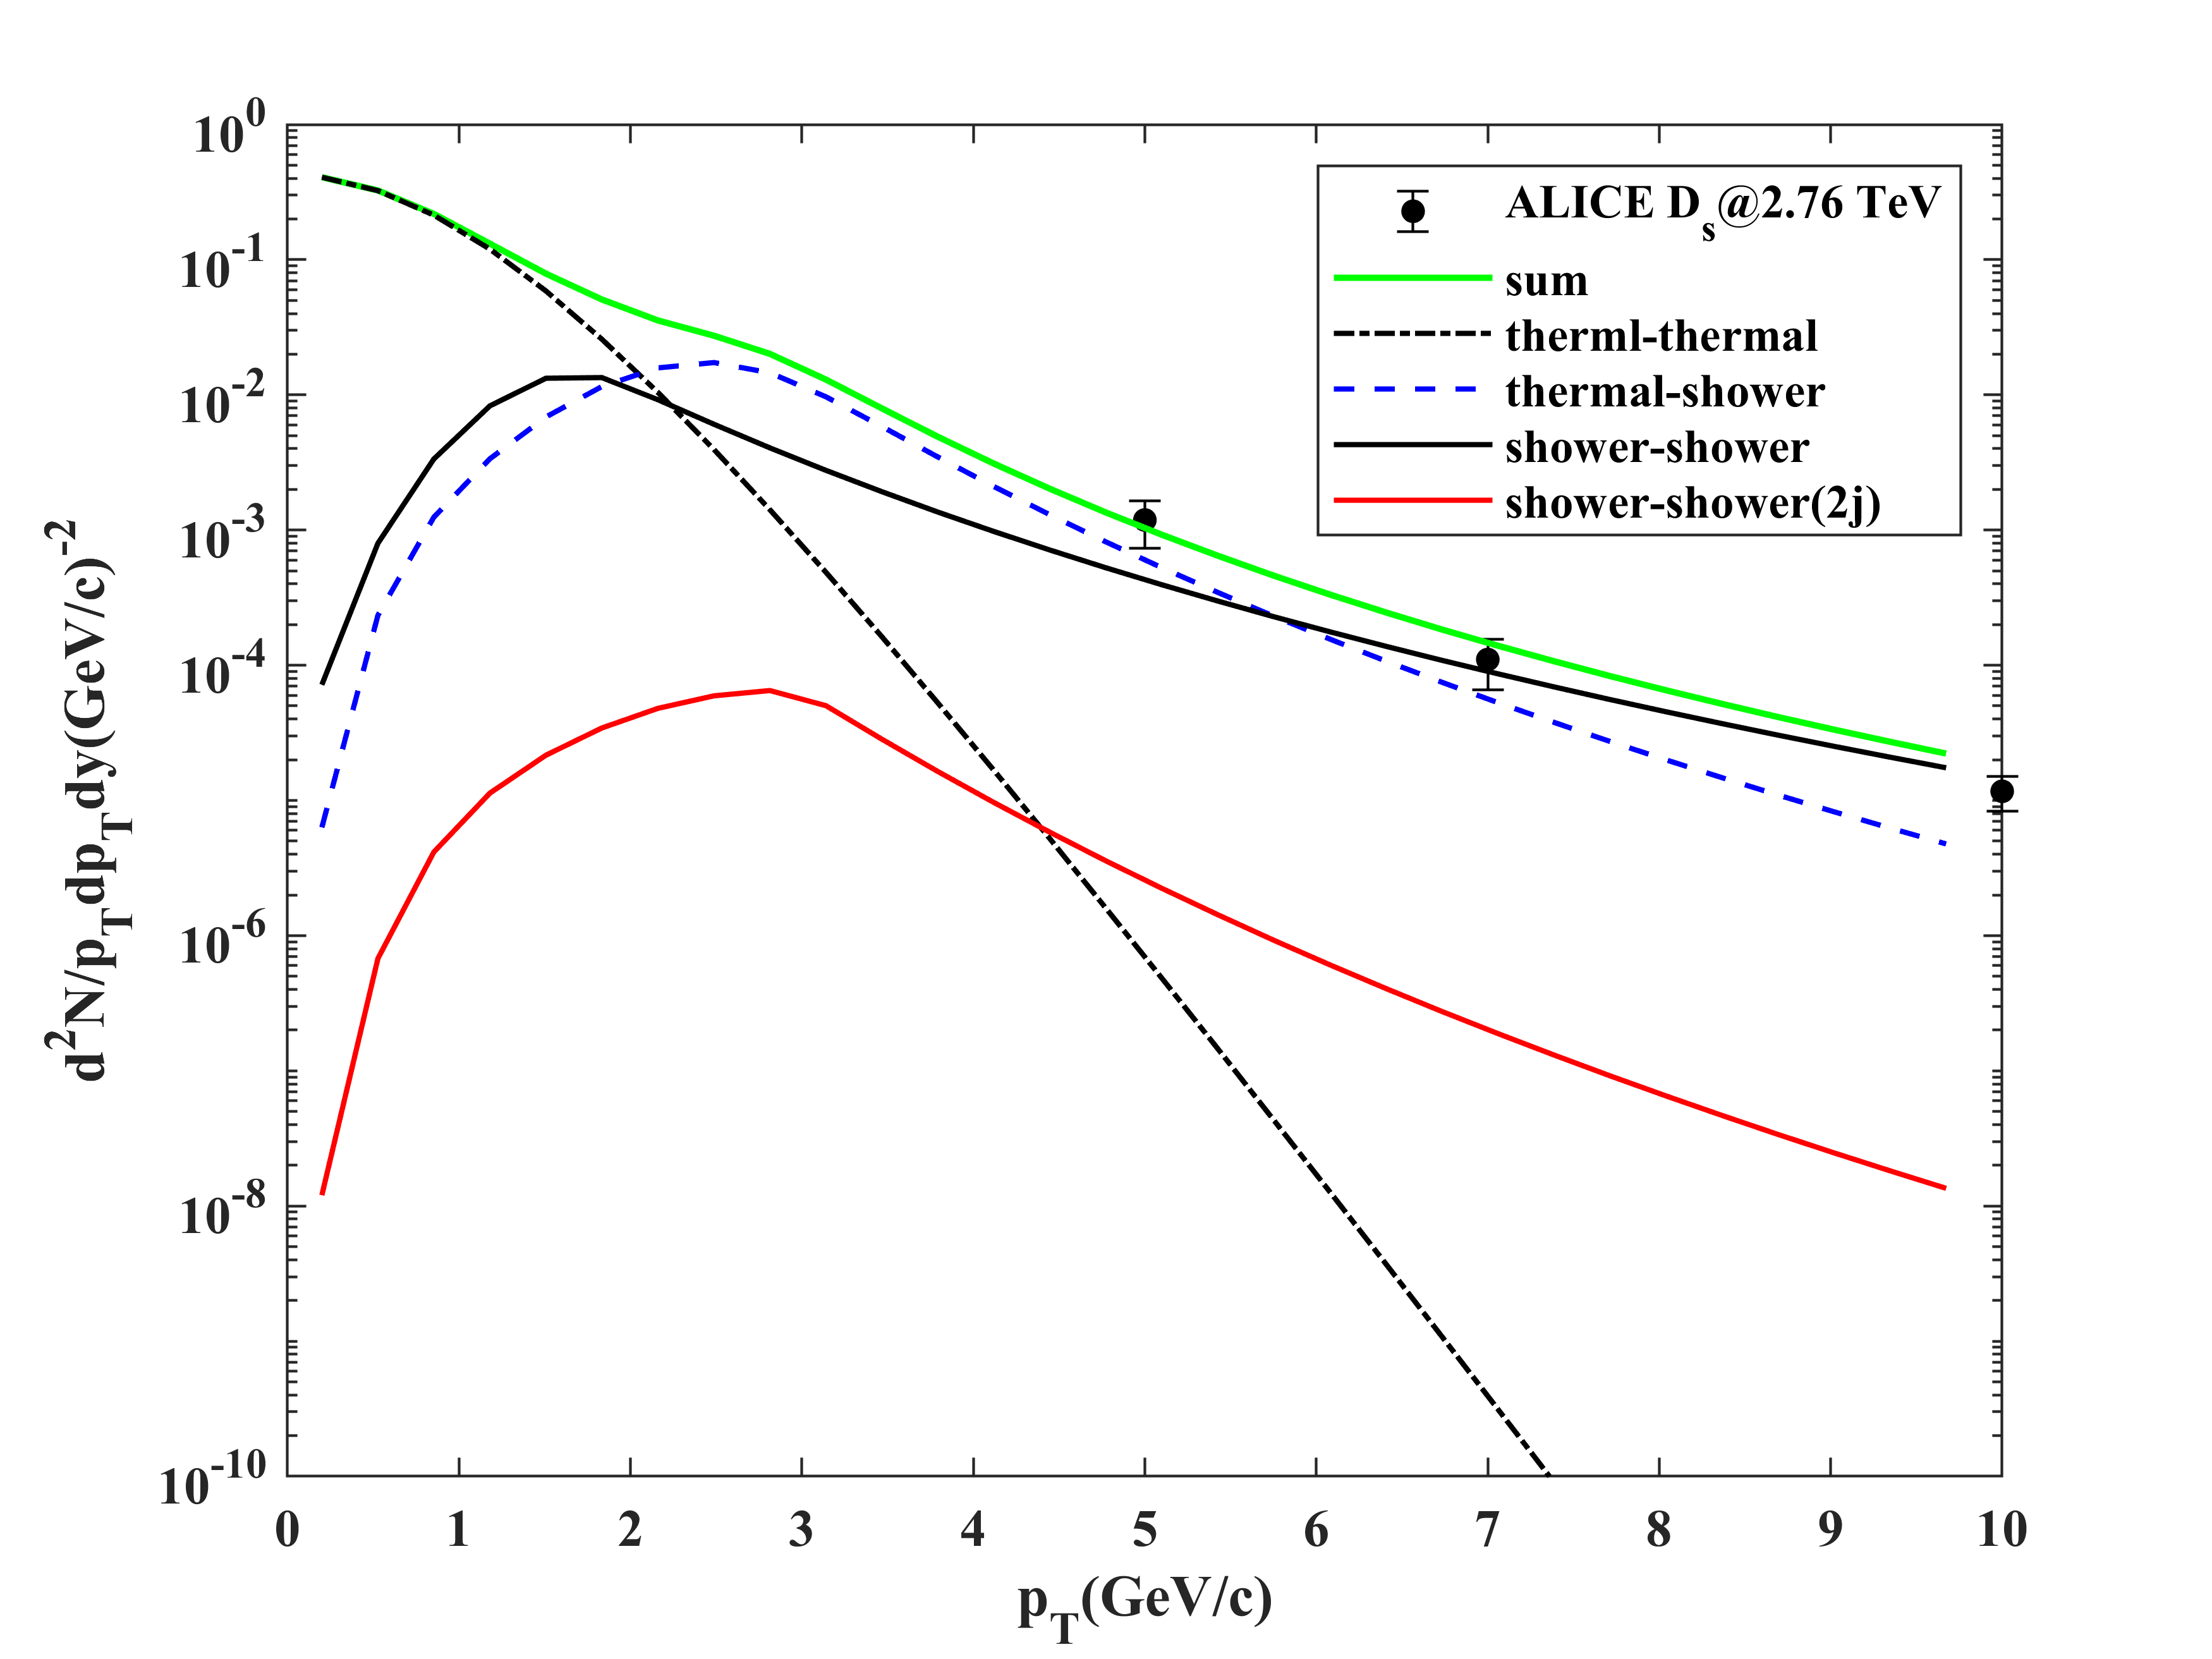
\includegraphics[width=0.45\textwidth]{Ds_1106.png}
	\caption{$D_s$ distribution at 2.76 TeV. }
	\label{fig25}
\end{figure}


\section{Meeting 2022.11.14}
So far, two main issues have been put forward. One is that initial charm quark distribution $f_c(k)$ at 2.76 and 5.02 TeV should be determined reasonably. Prof. Min He has recommended FONLL Heavy Quark Production program(\url{http://www.lpthe.jussieu.fr/~cacciari/fonll/fonllform.html}) to produce charm distributions in pp collisions at any energy, which can figure out this issue.

We first get the factor, by which charm distribution multiplied or (1/pi dsigma/dp^2/dy) divided, i.e. $3.2\times10^6$ at 5.5 TeV. Then the parameterized charm distribution can be derived.
\begin{eqnarray}
	\text{2.76 TeV: }\nonumber\\ 
	f_c(p_T)&=&\frac{dN_c}{d^2 p_T}\nonumber\\ 
	&=&\frac{\text{Exp}(20.406 - 3.343 p_T^{0.5})}{3.2\times10^6}\\
	\text{5.02 TeV: }\nonumber\\ 
	f_c(p_T)&=&\frac{dN_c}{d^2 p_T}\nonumber\\ 
	&=&\frac{\text{Exp}(20.49 - 3.15879 p_T^{0.5})}{3.2\times10^6}
\end{eqnarray}
 The fitted results are shown in Fig.\ref{fig26}.
\begin{figure}[H]
	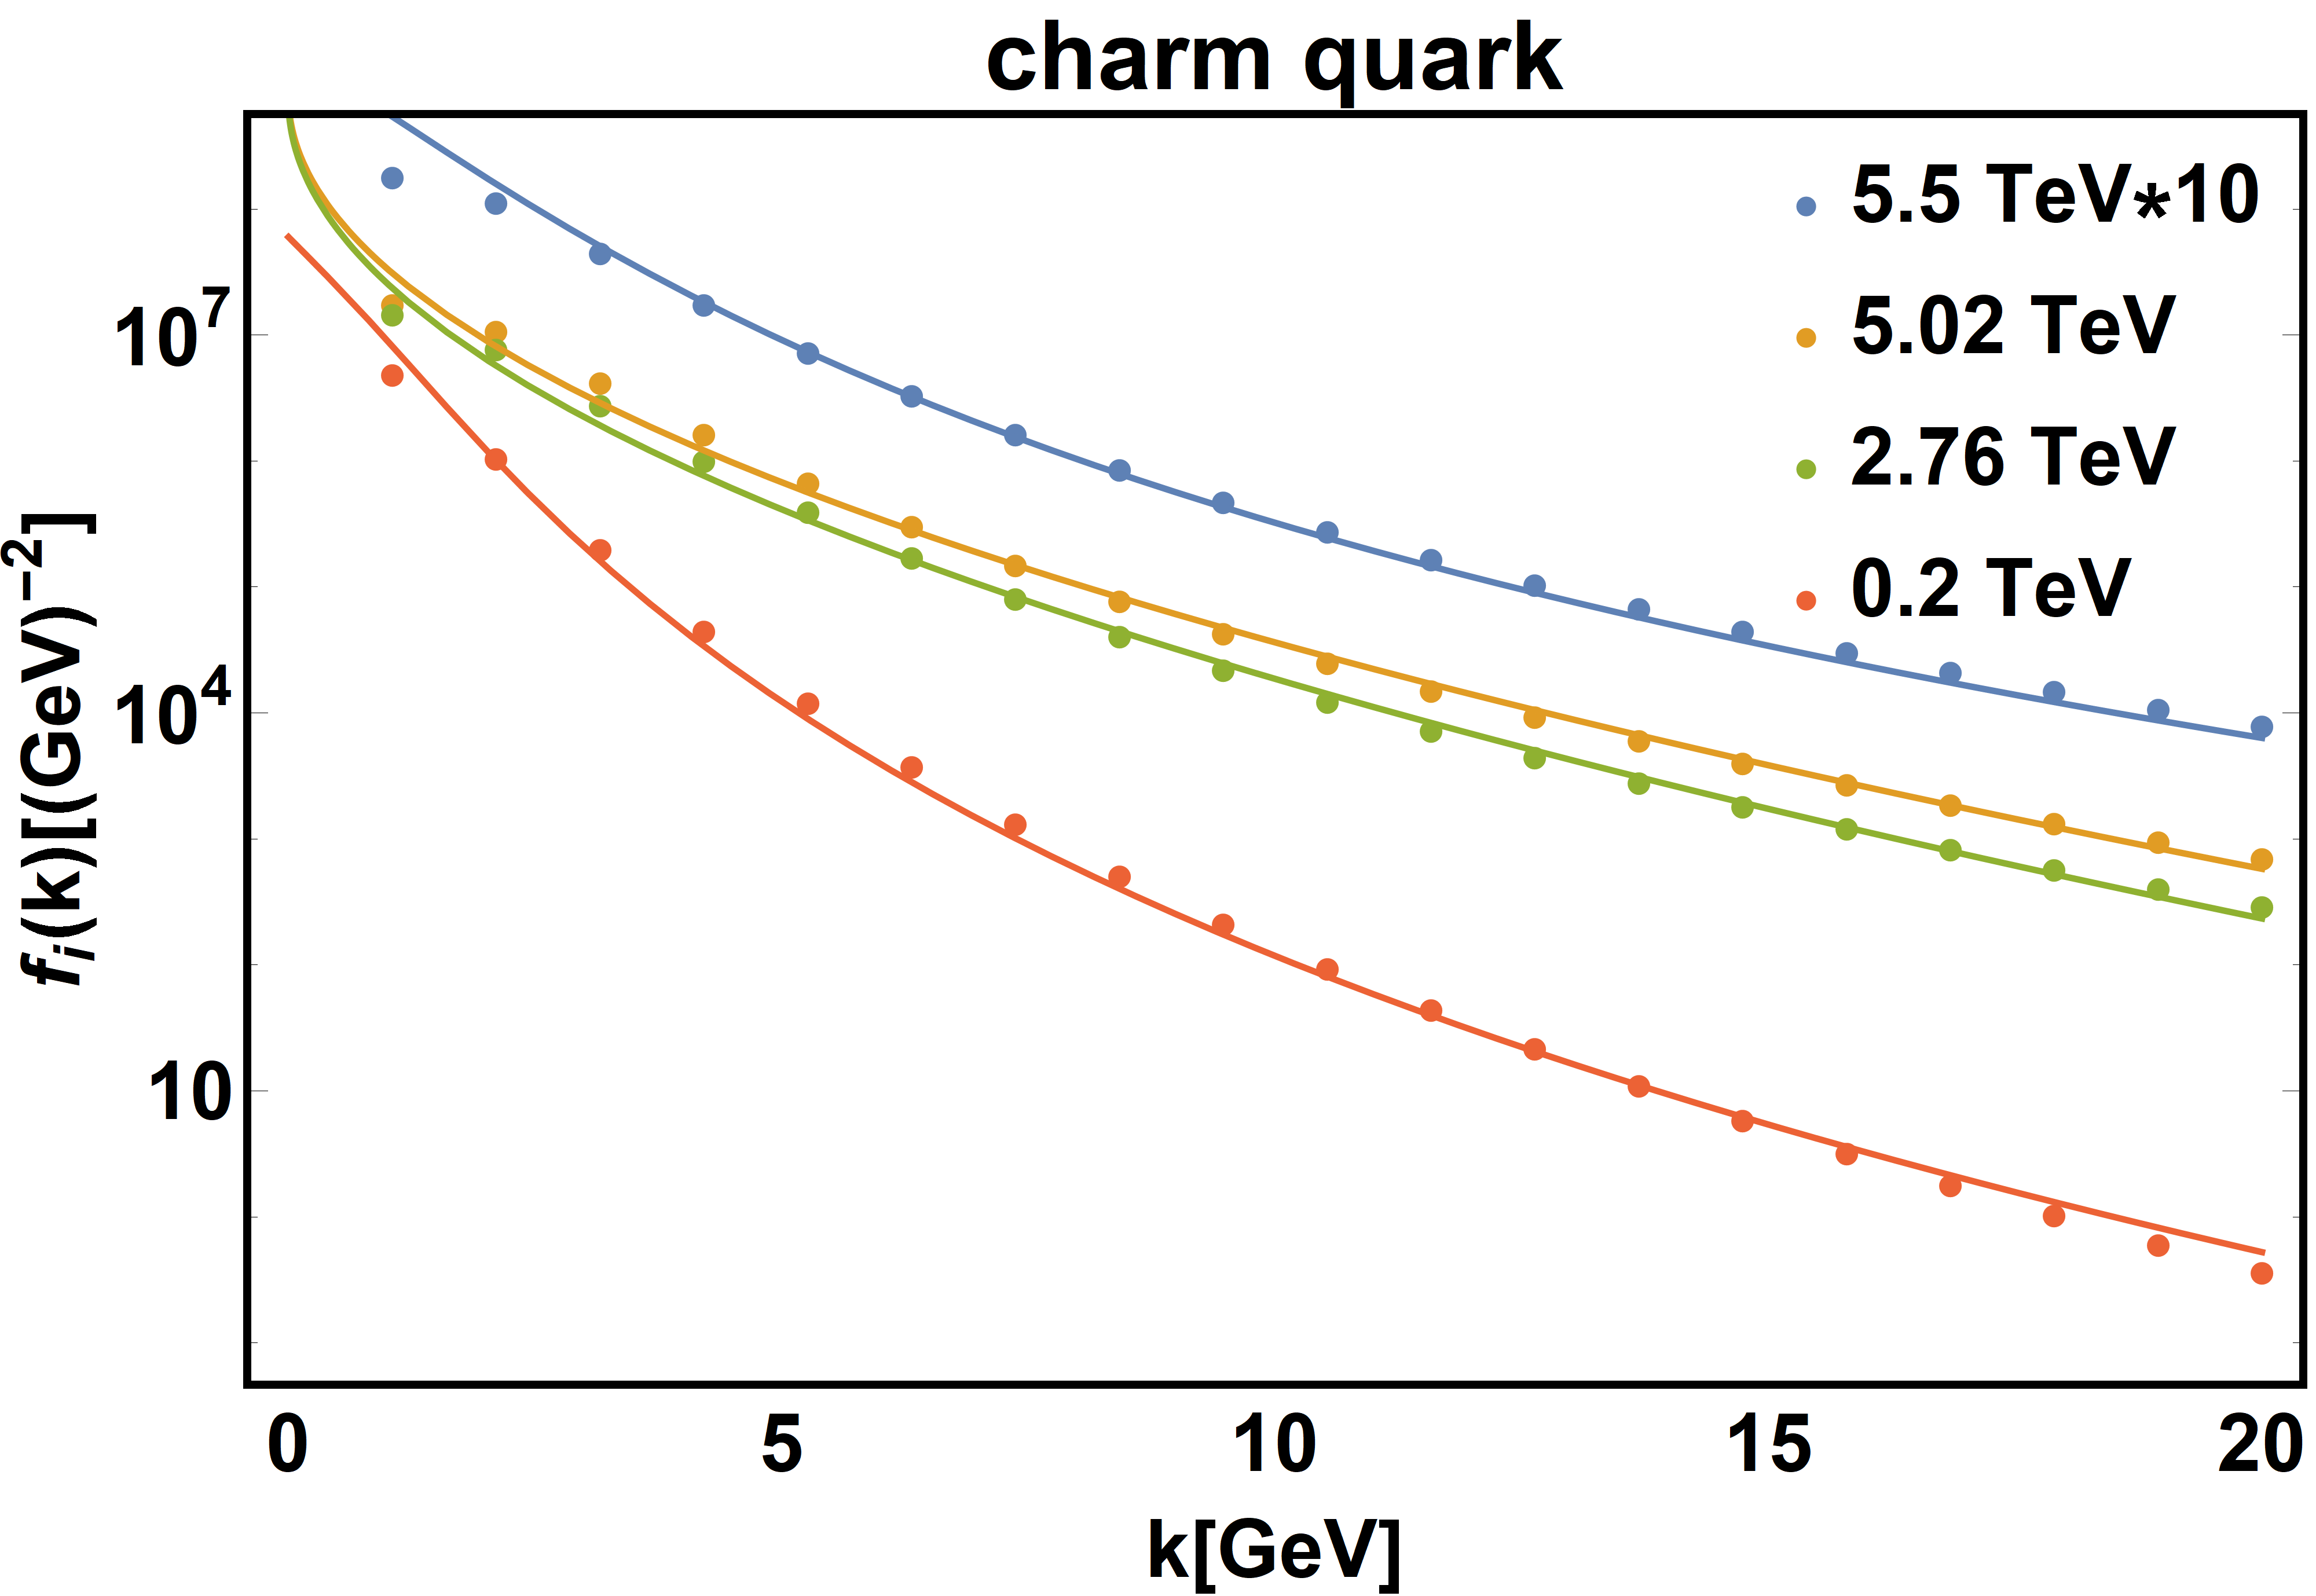
\includegraphics[width=0.45\textwidth]{FONLL.png}
	\caption{Charm quark distributions $f_c(k)$ fitted by FONLL data. }
	\label{fig26}
\end{figure}

Another is that which integral limits in terms of $SS(2j)$, described in Sec.\ref{integral issue}, should be adopted.

\section{MEETING 2022.11.28}
Now new $f_c(k)$ is adopted to reproduce charmed mesons. And new fitted parameters are listed here:
\begin{eqnarray}
	\text{2.76 TeV}&:&  \nonumber \\
	&&T=0.185 \text{ GeV}, \Gamma=10^{-2}, \nonumber \\
	&&\gamma_l=1.0,  \gamma_s=0.8 ,\gamma_c=0.26\nonumber \\
	J/\psi&:& v_T=0.25c,  \\ \nonumber
	&&\beta L\rightarrow \text{0 for charm, 2.39 for gluon}\nonumber\\
	D^0&:& v_T=0.43c,  \beta L=\text{3.5 for all}\nonumber\\
	D_s&:& v_T=0.3c,    \beta L=\text{2.9 for all}.\nonumber\\
	\text{5.02 TeV}&:&  \nonumber \\
	&&T=0.185 \text{ GeV}, \Gamma=10^{-2}, \nonumber \\
	&&\gamma_l=0.5,  \gamma_s=0.3 ,\gamma_c=0.49\nonumber \\
	J/\psi&:& v_T=0.28c,  \\ \nonumber
	&&\beta L\rightarrow \text{0 for charm, 0.8 for gluon}\nonumber\\
	D^0&:& v_T=0.51c,  \beta L=\text{3.0 for charm, 7.0 for gluon}\nonumber\\
	D_s&:& v_T=0.2c,    \beta L=\text{2.0 for charm, 6.0 for gluon}.\nonumber
\end{eqnarray}
Through those above, the spectra are shown below.

\begin{figure}[H]
	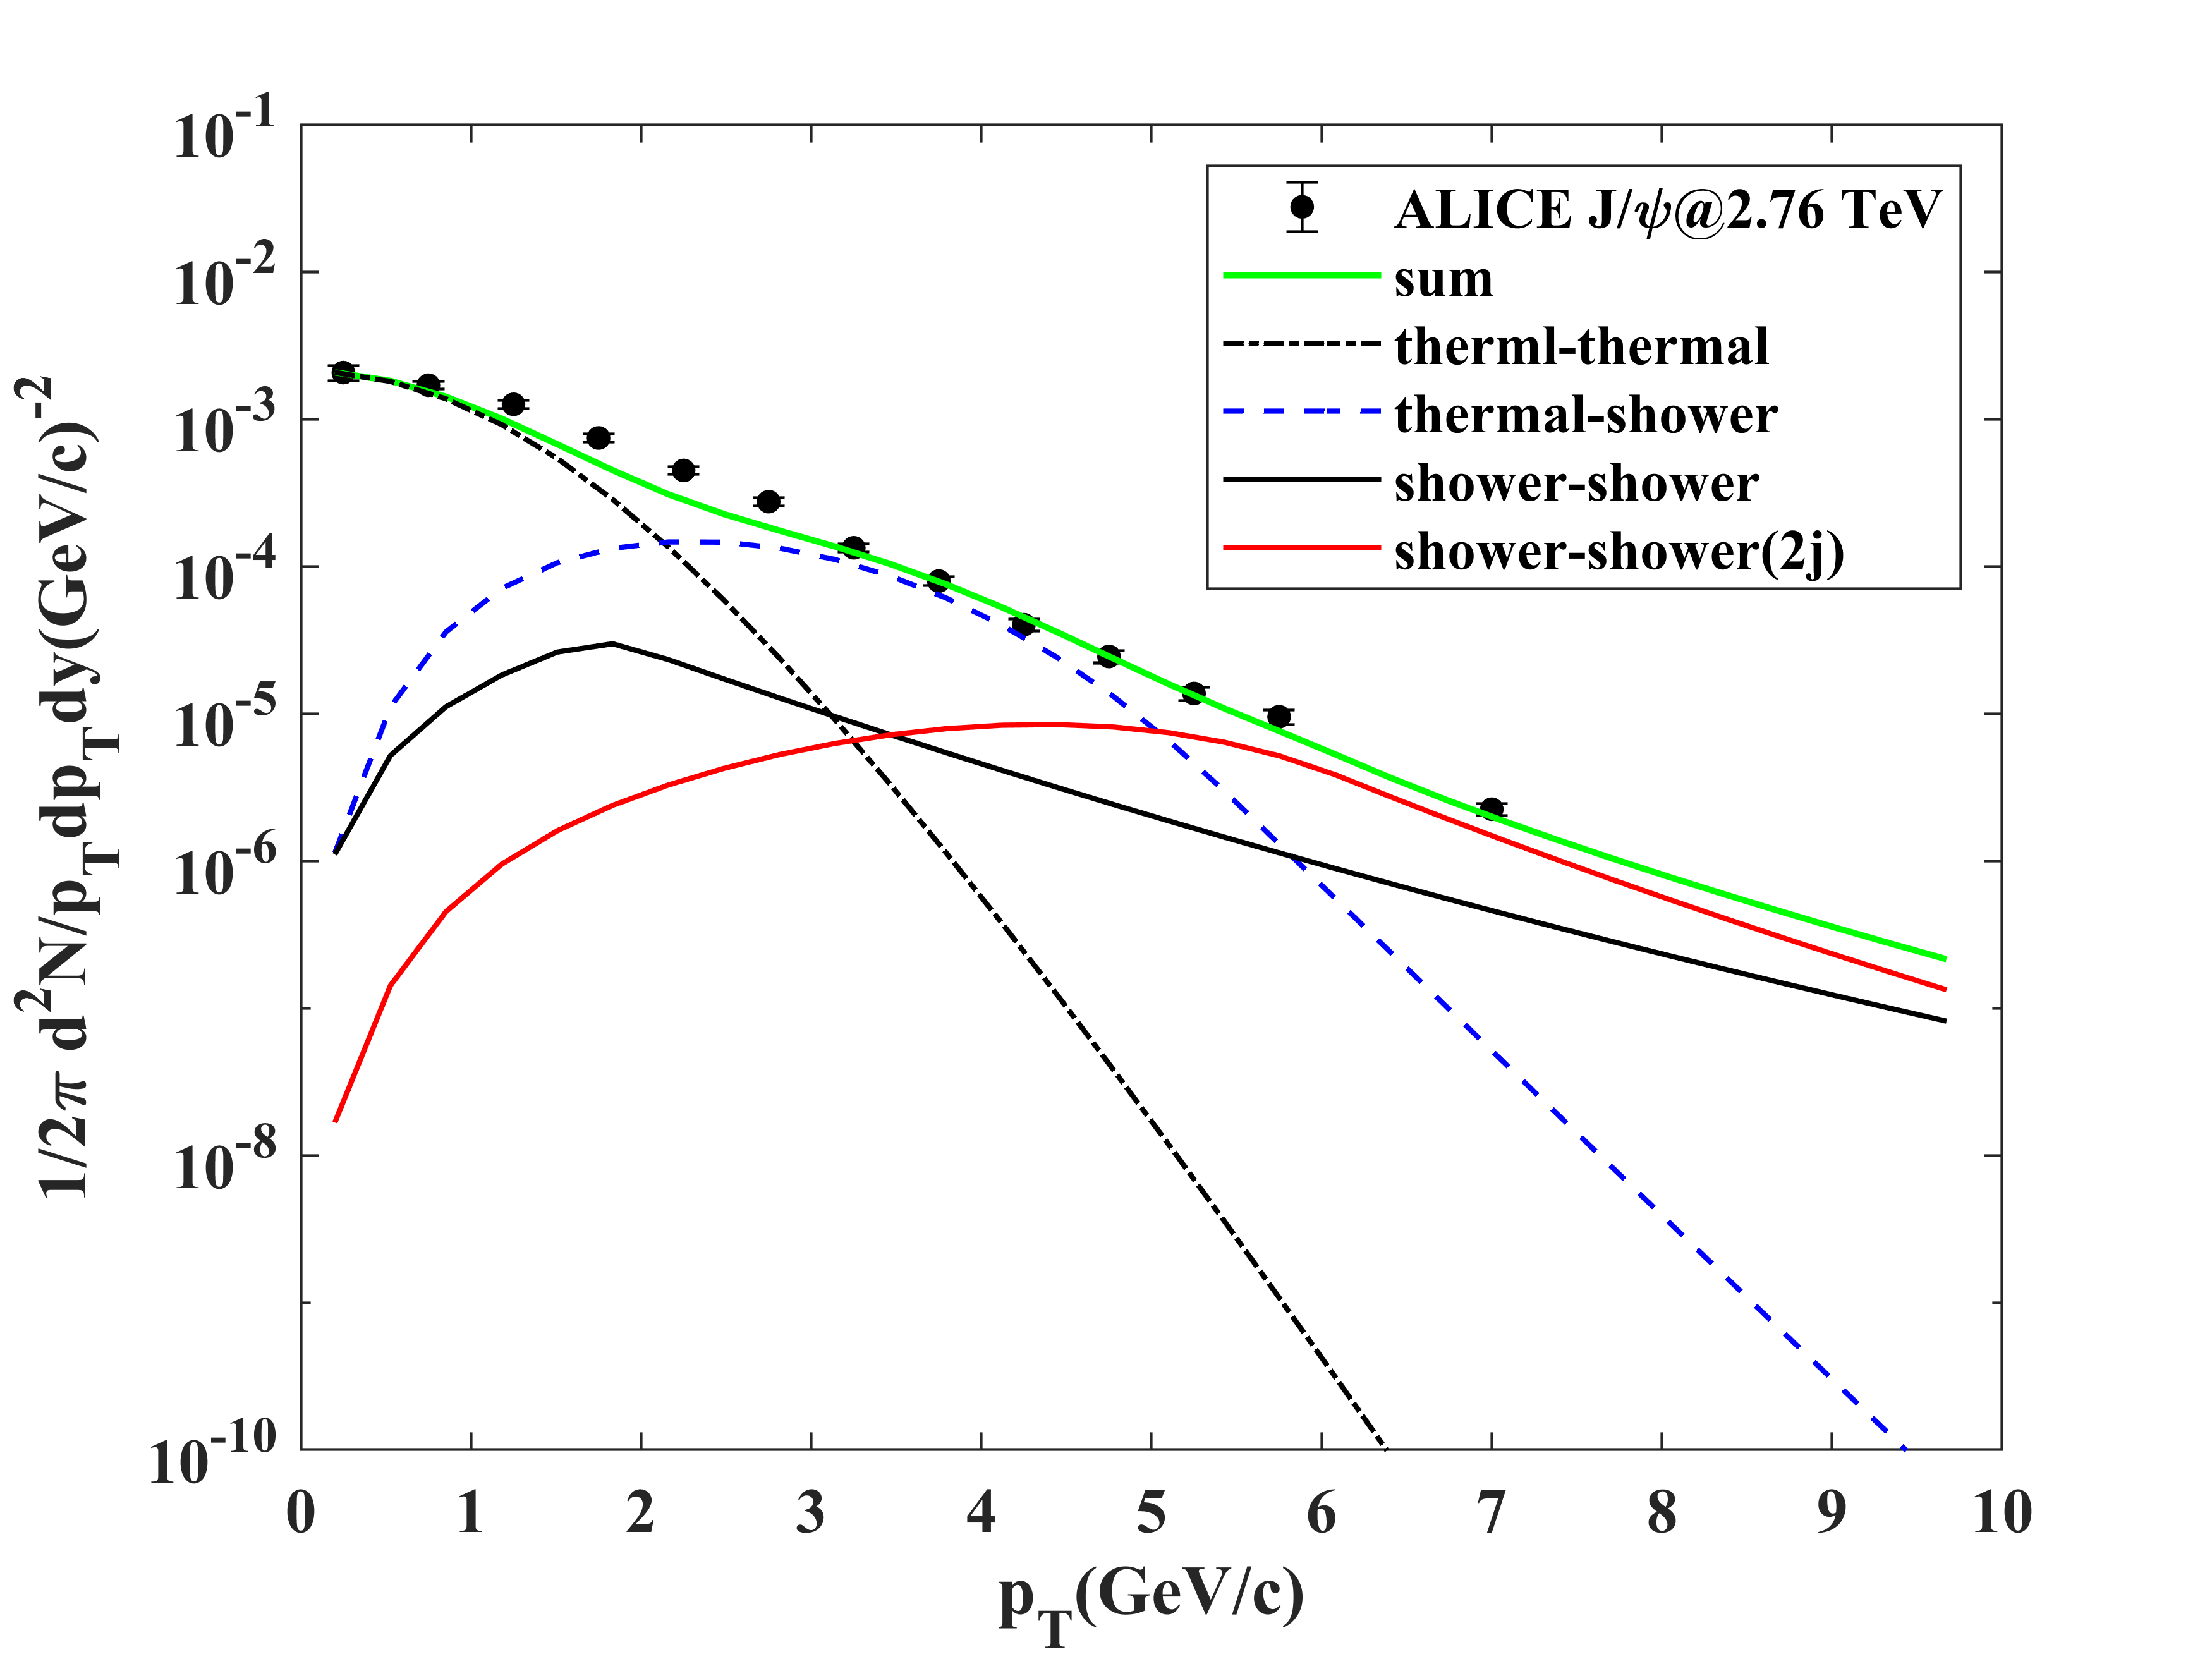
\includegraphics[width=0.45\textwidth]{Jpsi276_FONLL.png}
	\caption{$J/\psi$ distribution at 2.76 TeV. }
	\label{fig27}
\end{figure}
\begin{figure}[H]
	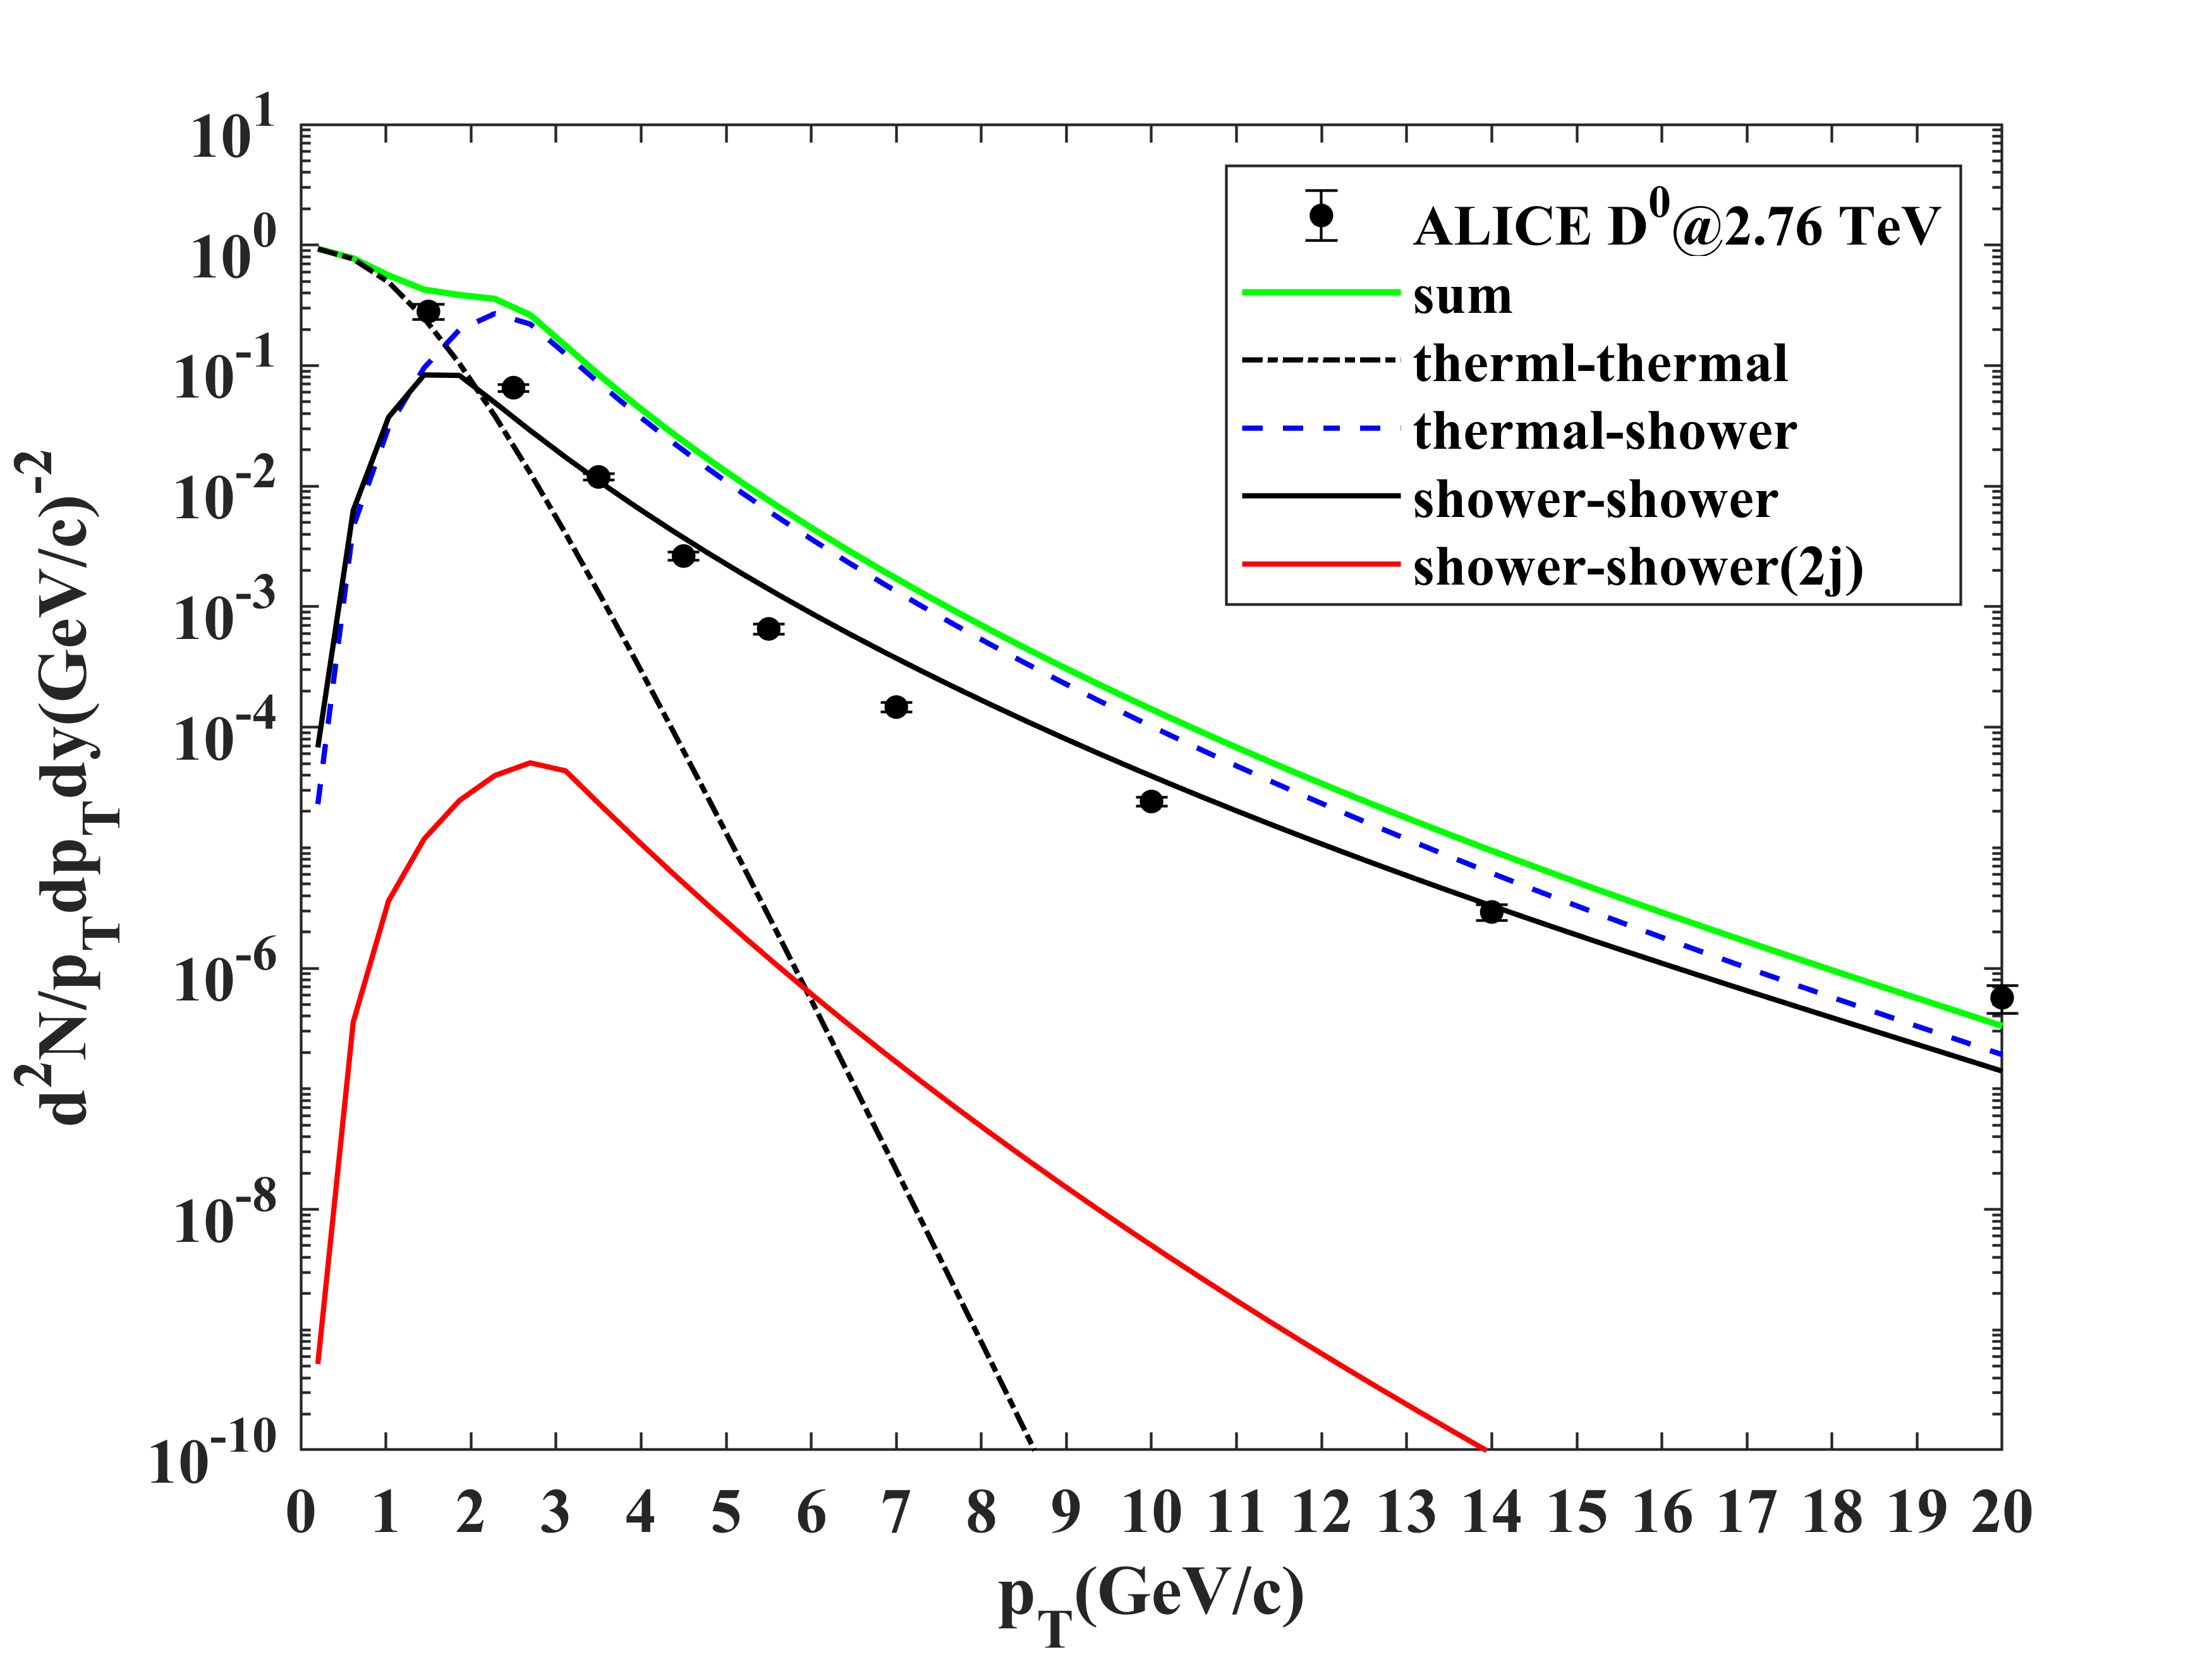
\includegraphics[width=0.45\textwidth]{D0276_FONLL.png}
	\caption{$D^0$ distribution at 2.76 TeV. }
	\label{fig28}
\end{figure}
\begin{figure}[H]
	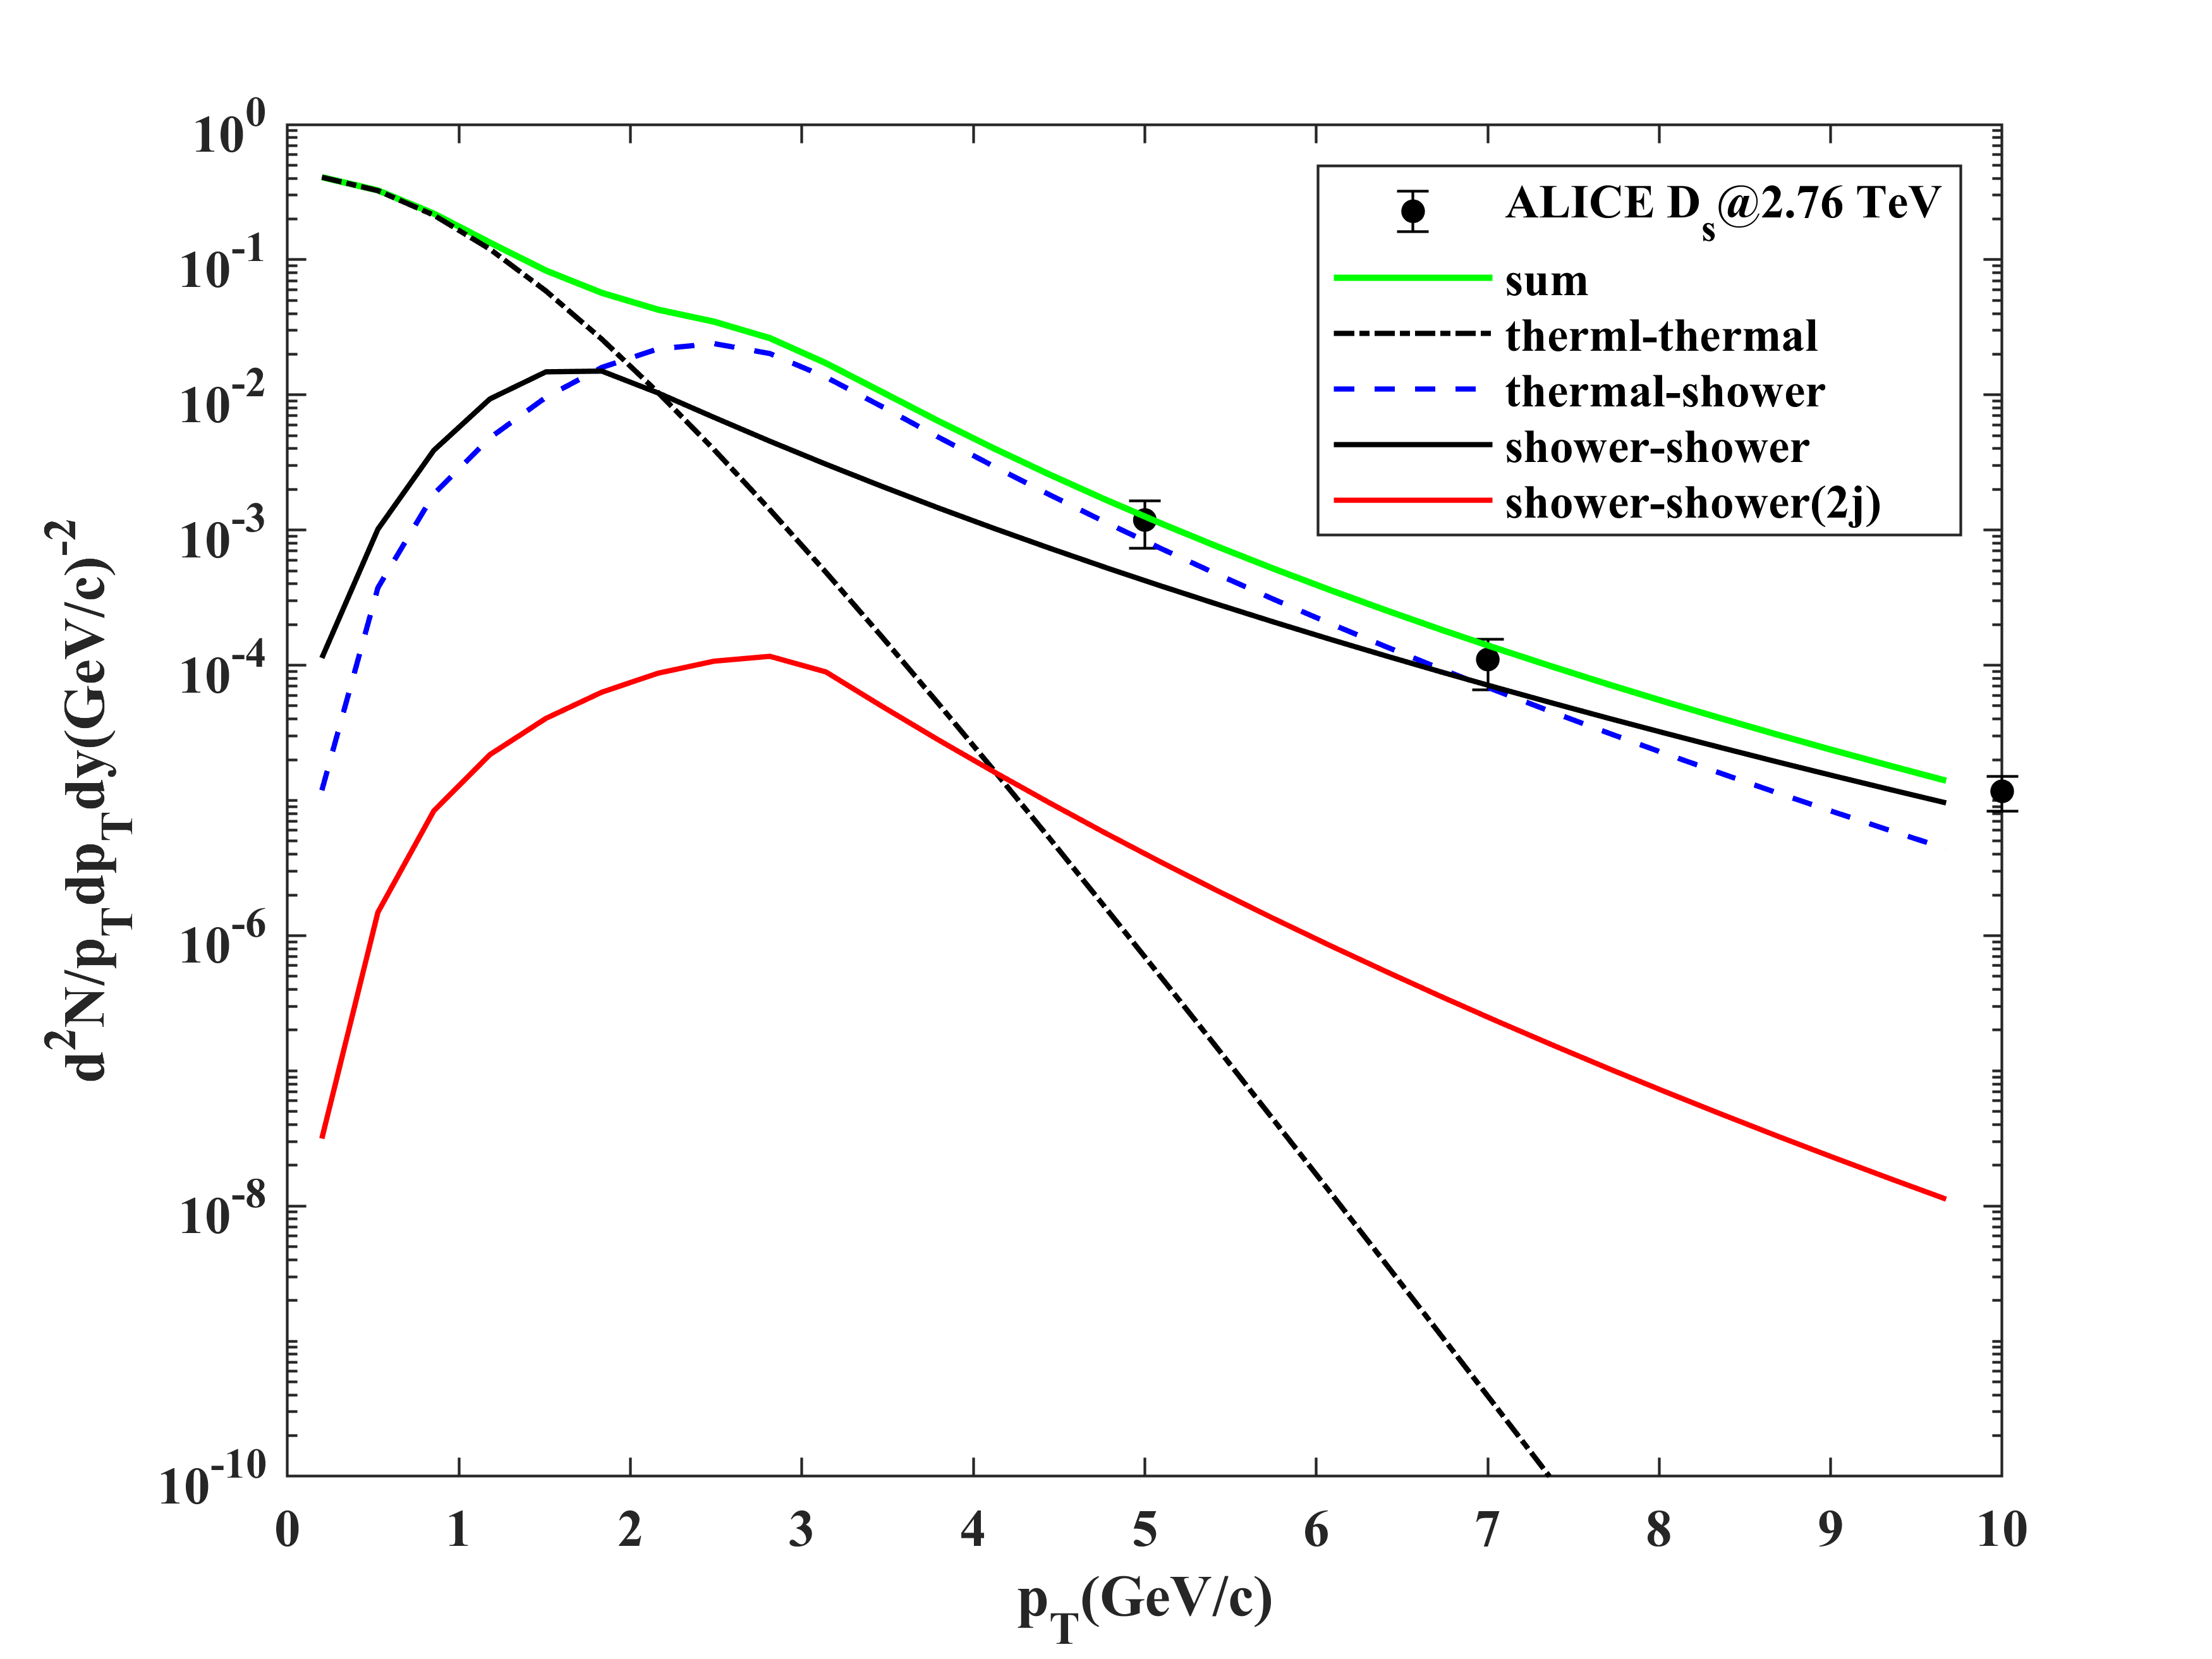
\includegraphics[width=0.45\textwidth]{Ds276_FONLL.png}
	\caption{$D_s$ distribution at 2.76 TeV. }
	\label{fig29}
\end{figure}

\begin{figure}[H]
	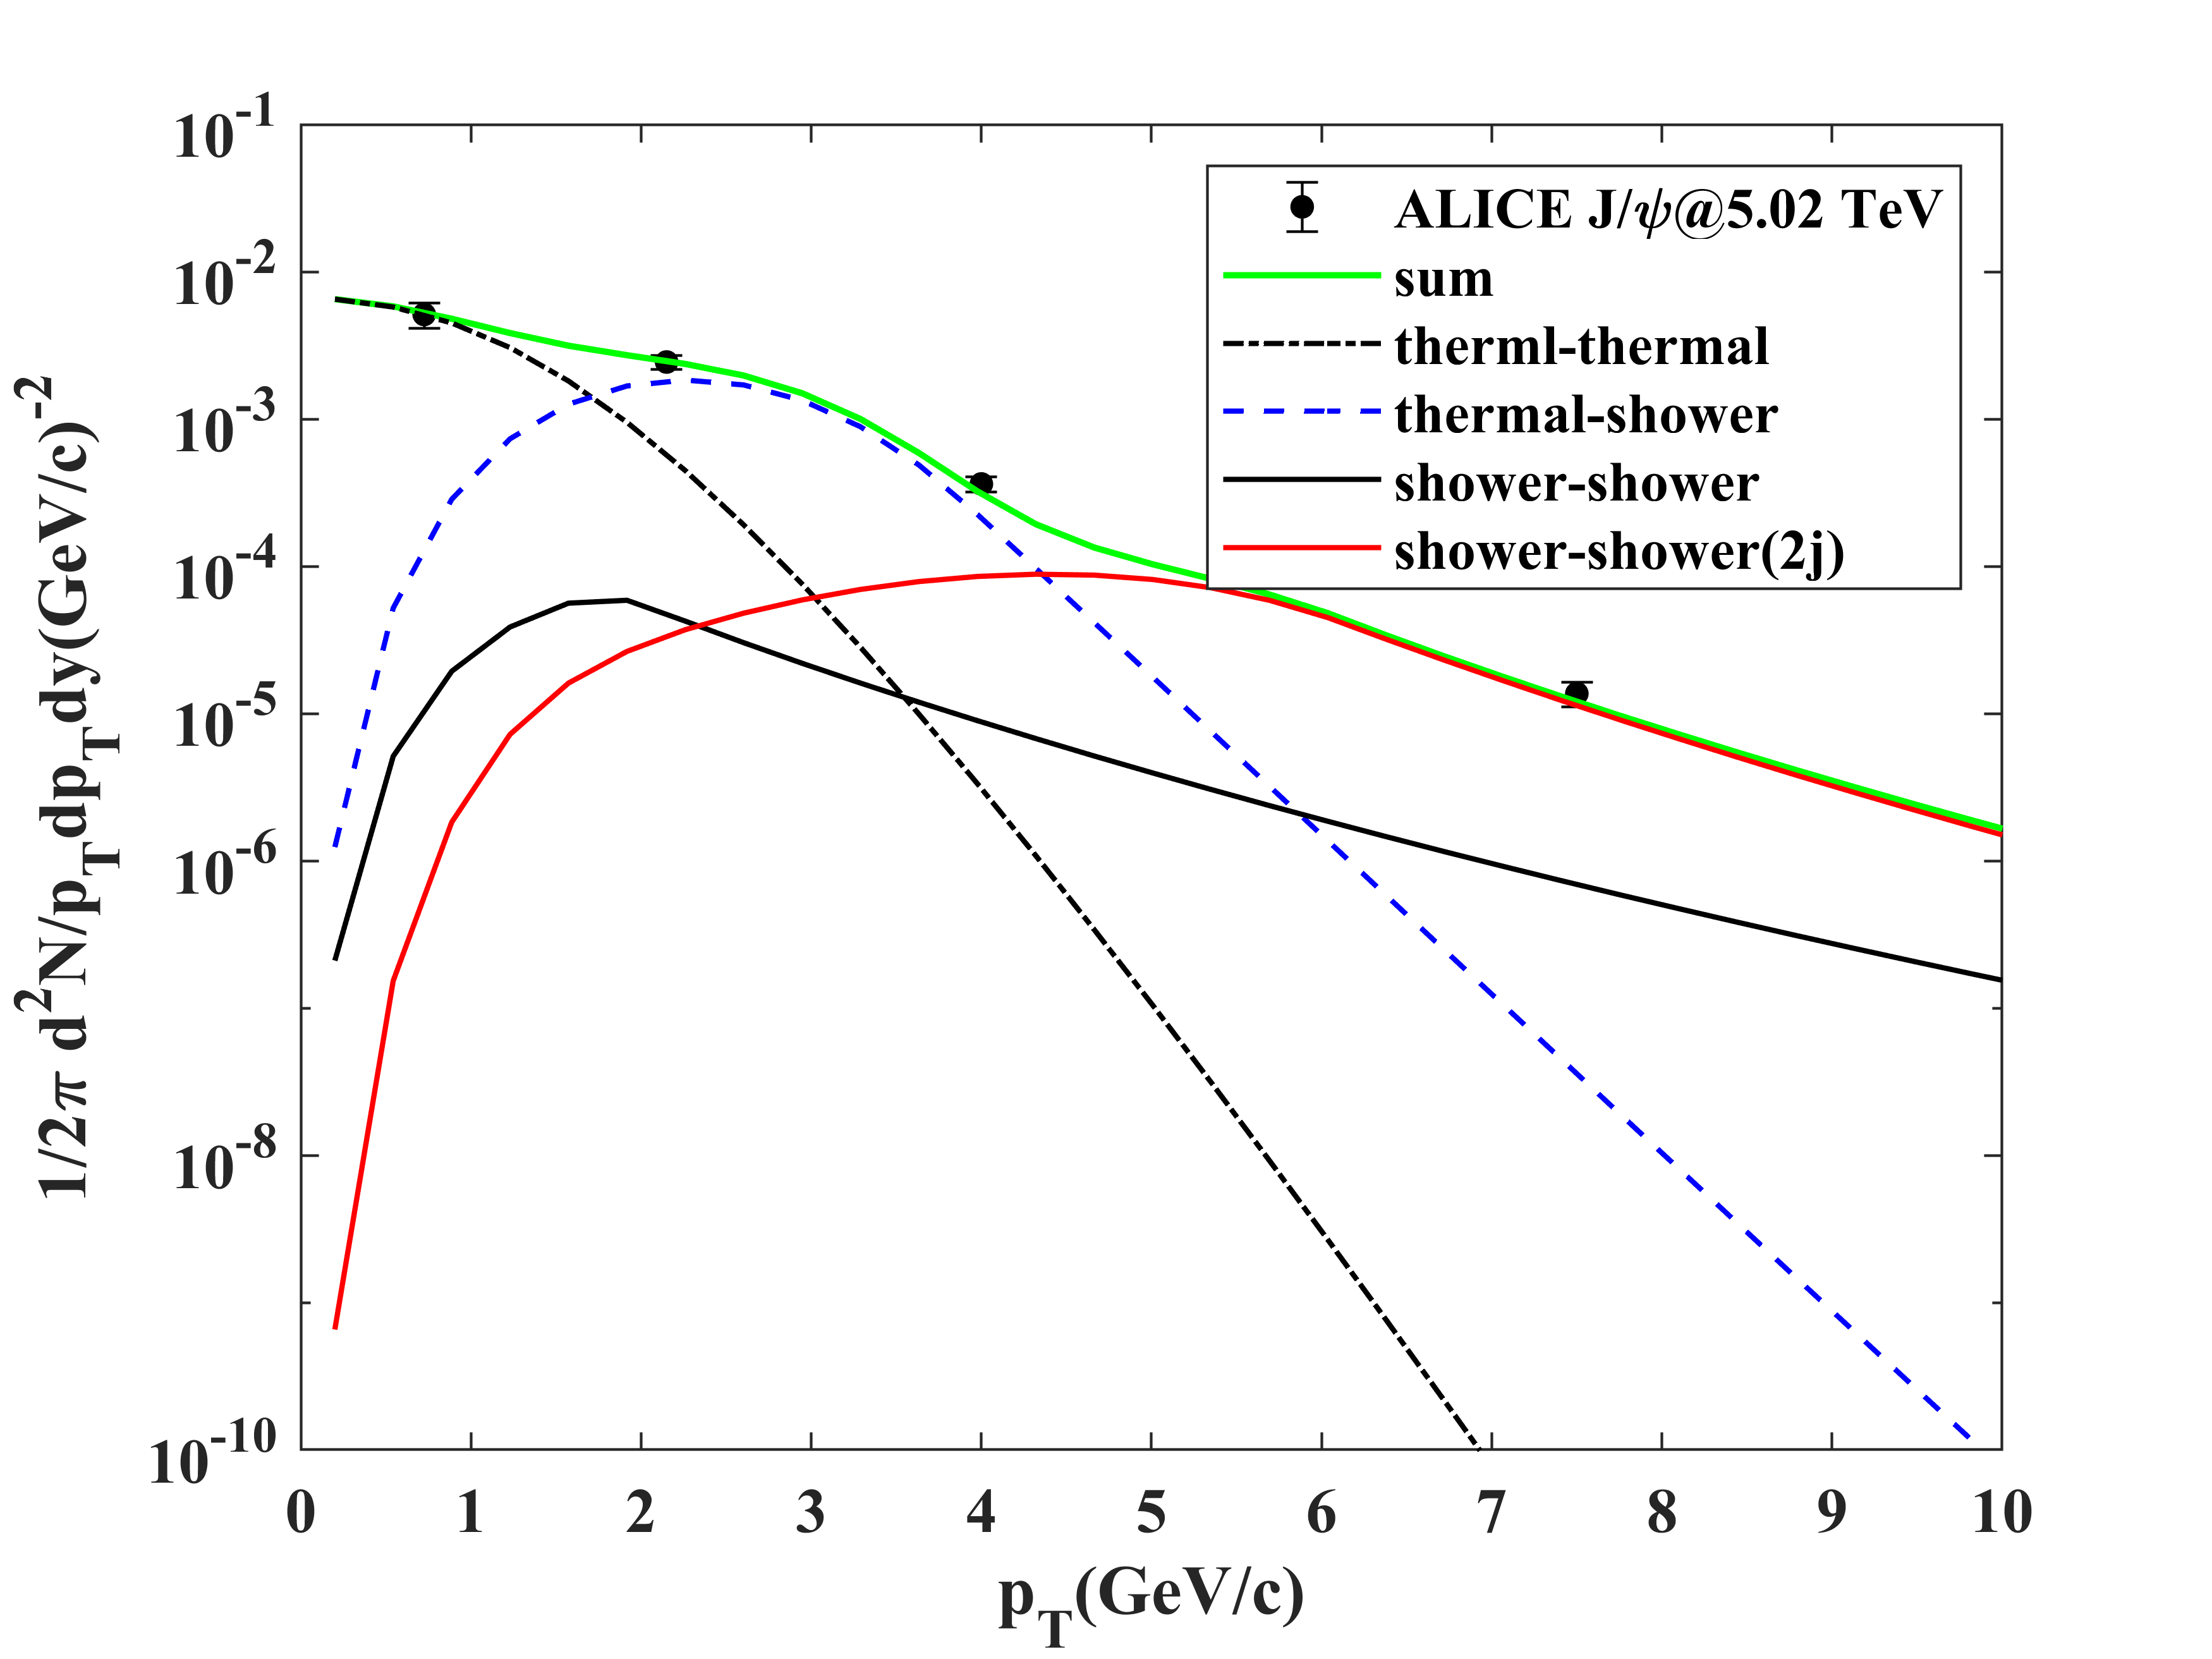
\includegraphics[width=0.45\textwidth]{Jpsi502_FONLL.png}
	\caption{$J/\psi$ distribution at 5.02 TeV. }
	\label{fig30}
\end{figure}
\begin{figure}[H]
	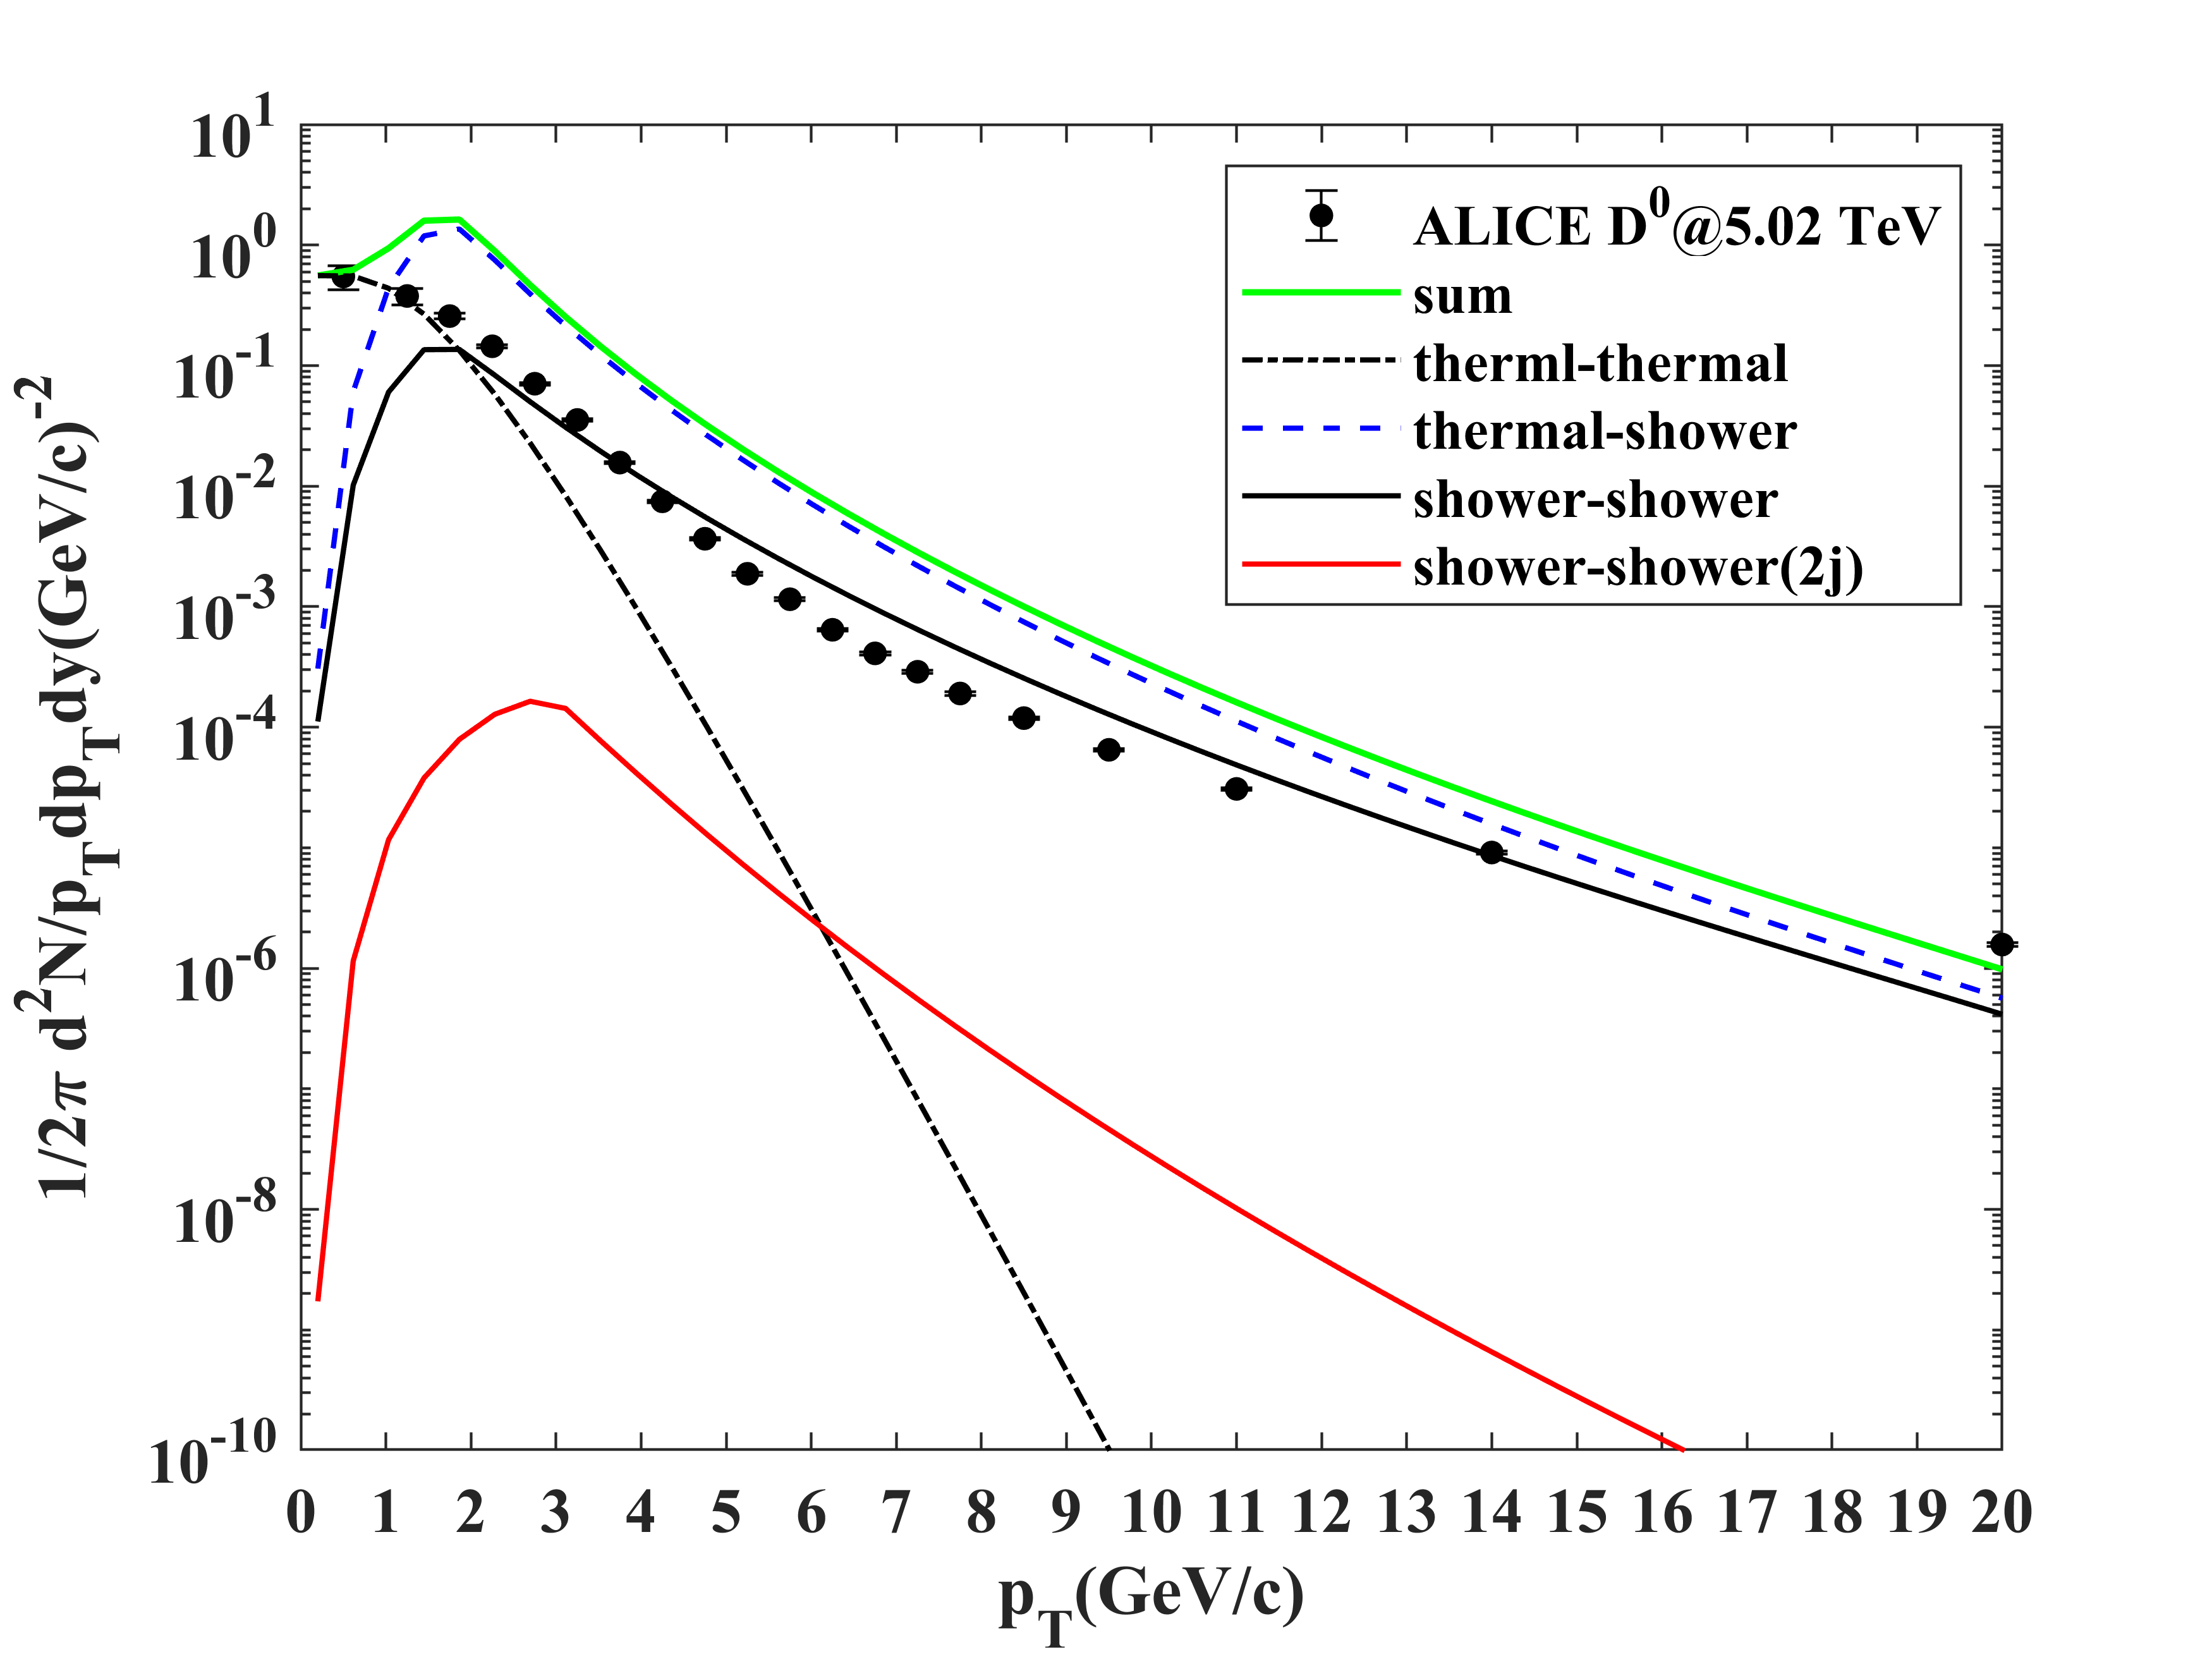
\includegraphics[width=0.45\textwidth]{D0502_FONLL.png}
	\caption{$D^0$ distribution at 5.02 TeV. }
	\label{fig31}
\end{figure}
\begin{figure}[H]
	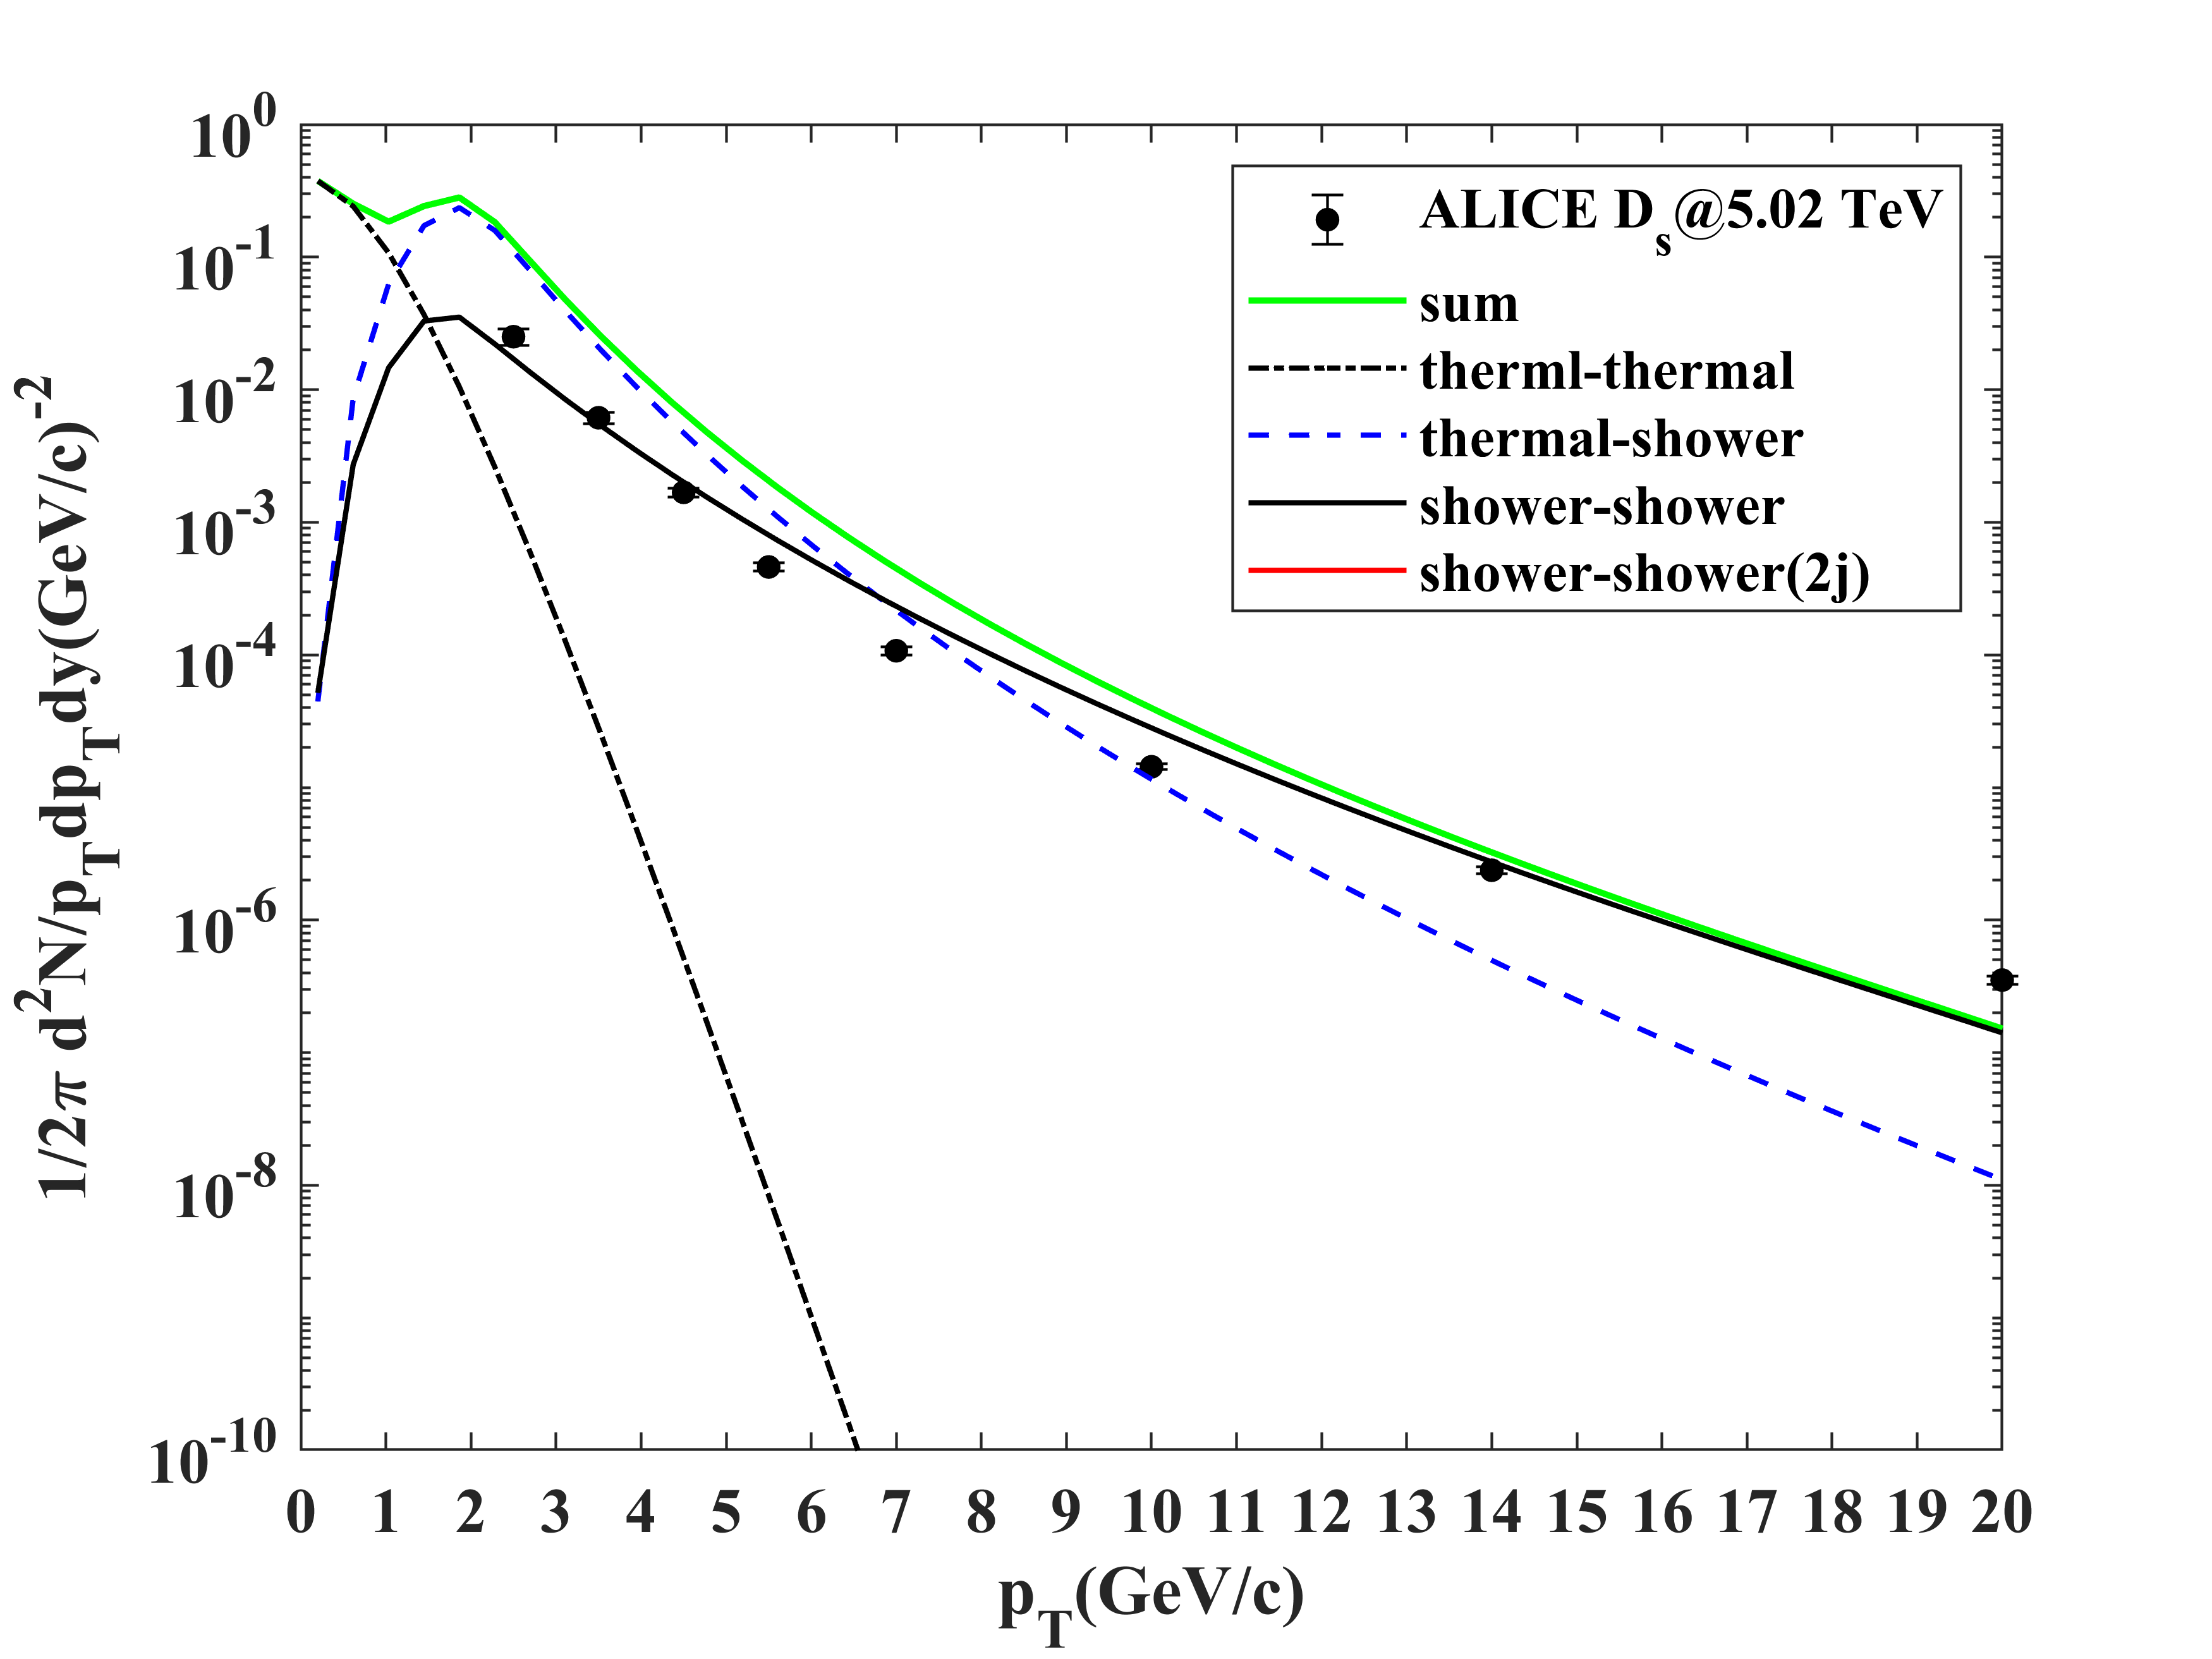
\includegraphics[width=0.45\textwidth]{Ds502_FONLL.png}
	\caption{$D_s$ distribution at 5.02 TeV. }
	\label{fig32}
\end{figure}

Next, we will check whether initial charm quark distribution is normalized and use $\itshape{recomb\_product\_v15.f90}$ to compare with last results to figure out SS(2j) integral issues.


\section{MEETING 2022.12.05}
Last week, by integration, we have found initial charm quark distribution is not normalized, so that the factor 3.2$\times 10^6$ is multiplied by direct.  And the results using $\itshape{recomb\_product\_v15.f90}$ are shown in Fig.\ref{fig33}.

To calculate Jpsi by changing phi program: p0:m(Jpsi)=3.096, fik:index 6、7 are note changed, however, fik has been changed.
Questions: gbst=0.432 ? Cs? C? T? Ts? anything else not changed.
\begin{figure}[H]
	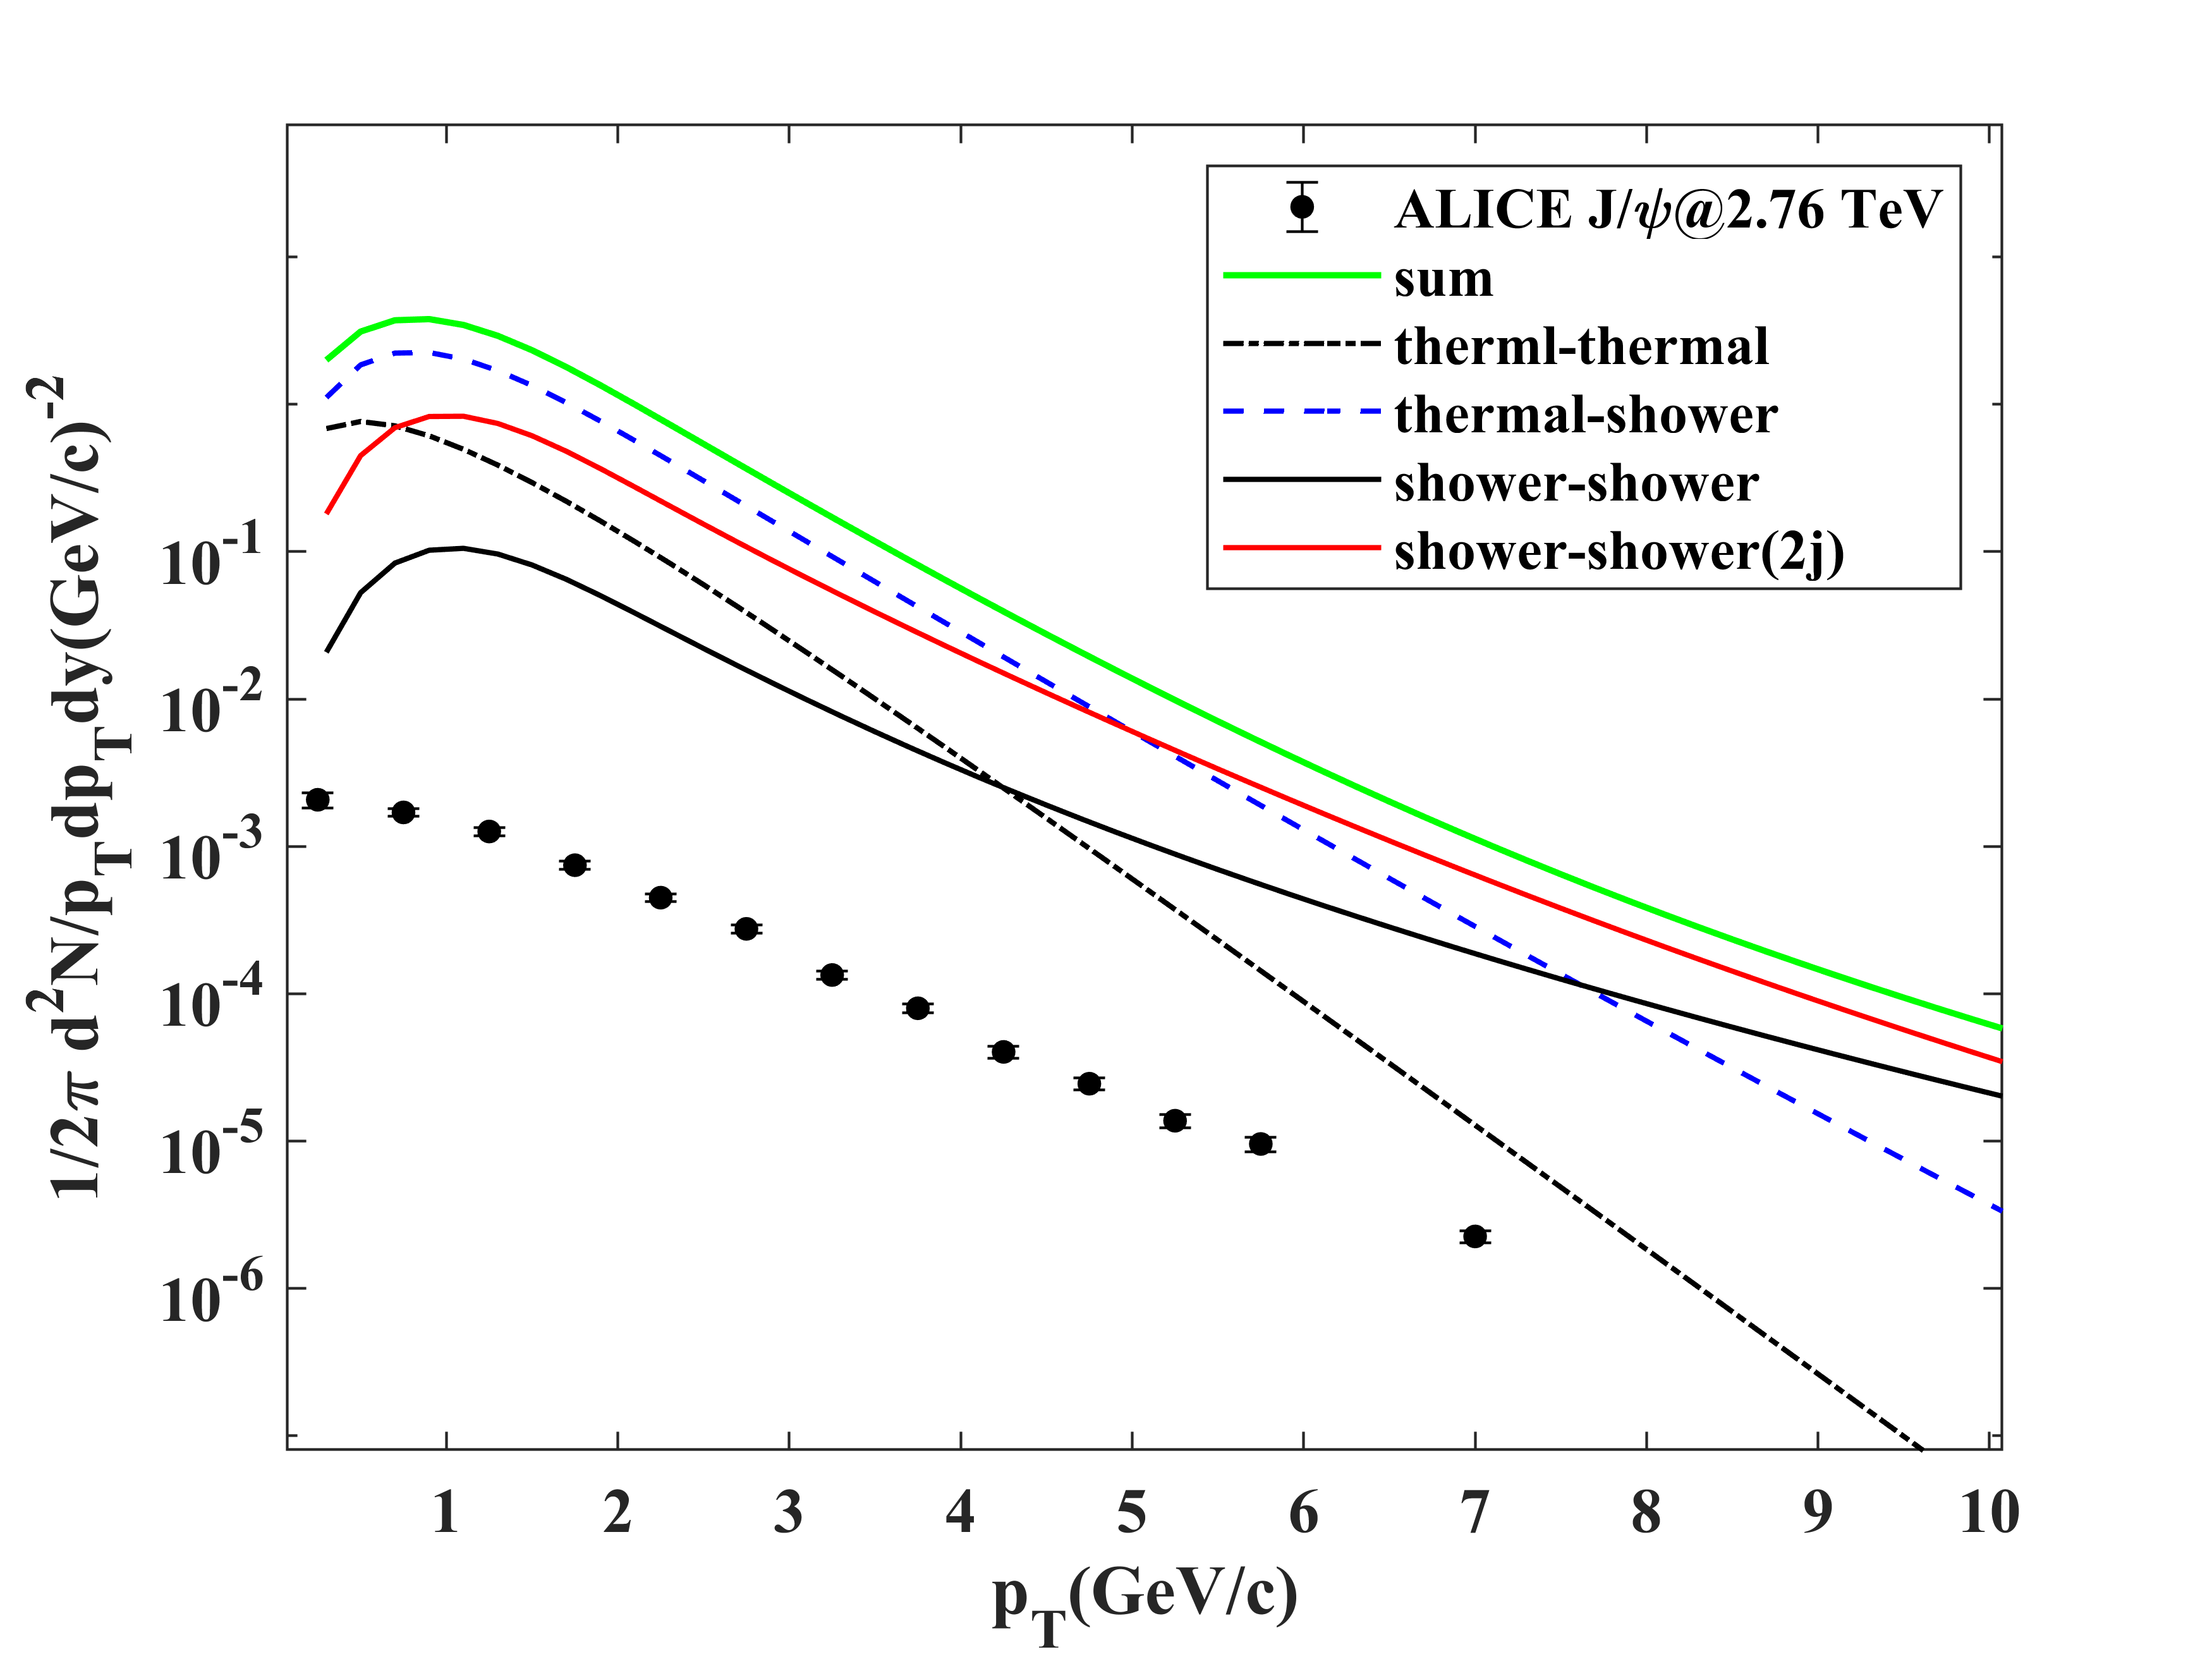
\includegraphics[width=0.45\textwidth]{Jpsi276_Zhu.png}
	\caption{$J/\psi$ distribution at 2.76 TeV using \itshape{recomb\_product\_v15.f90}. }
	\label{fig33}
\end{figure}

Then, due to various framework compared with recombination model, we only adopt $SS(2j)$ in version15 program.

\section{MEETING 2022.12.12}
This week, first, considering inconsistent asymptotic behavior of charm jet distribution at low momentum, its contribution is cut off by a smooth function, like Fermi-Dirac distribution, which we take to be \cite{PhysRevC.84.064914} for gluon
\begin{eqnarray}
	g(q)=[1+e^{(3.5-q)/0.5}]^{-1}.\label{QuenchFiqc}
\end{eqnarray}
Similarly, charm jet distributions can be given below, shown in \ref{fig34}.
 \begin{eqnarray}
 	\text{2.76 TeV: }\nonumber\\ 
 	f_c(p_T)&=&\frac{dN_c}{d^2 p_T}\nonumber\\ 
 	&=&\frac{\text{Exp}(20.406 - 3.343 p_T^{0.5})}{3.5\times10^6}\nonumber\\
 	&&\times \frac{1}{1+e^{\frac{0.84-p_T}{0.257}}}\\ \label{fit_276}
 	\text{5.02 TeV: }\nonumber\\ 
 	f_c(p_T)&=&\frac{dN_c}{d^2 p_T}\nonumber\\ 
 	&=&\frac{\text{Exp}(20.49 - 3.15879 p_T^{0.5})}{3.5\times10^6}\nonumber\\
 	&&\times \frac{1}{1+e^{\frac{1.05-p_T}{0.3}}}  \label{fit_502}
 \end{eqnarray}

\begin{figure}[H]
	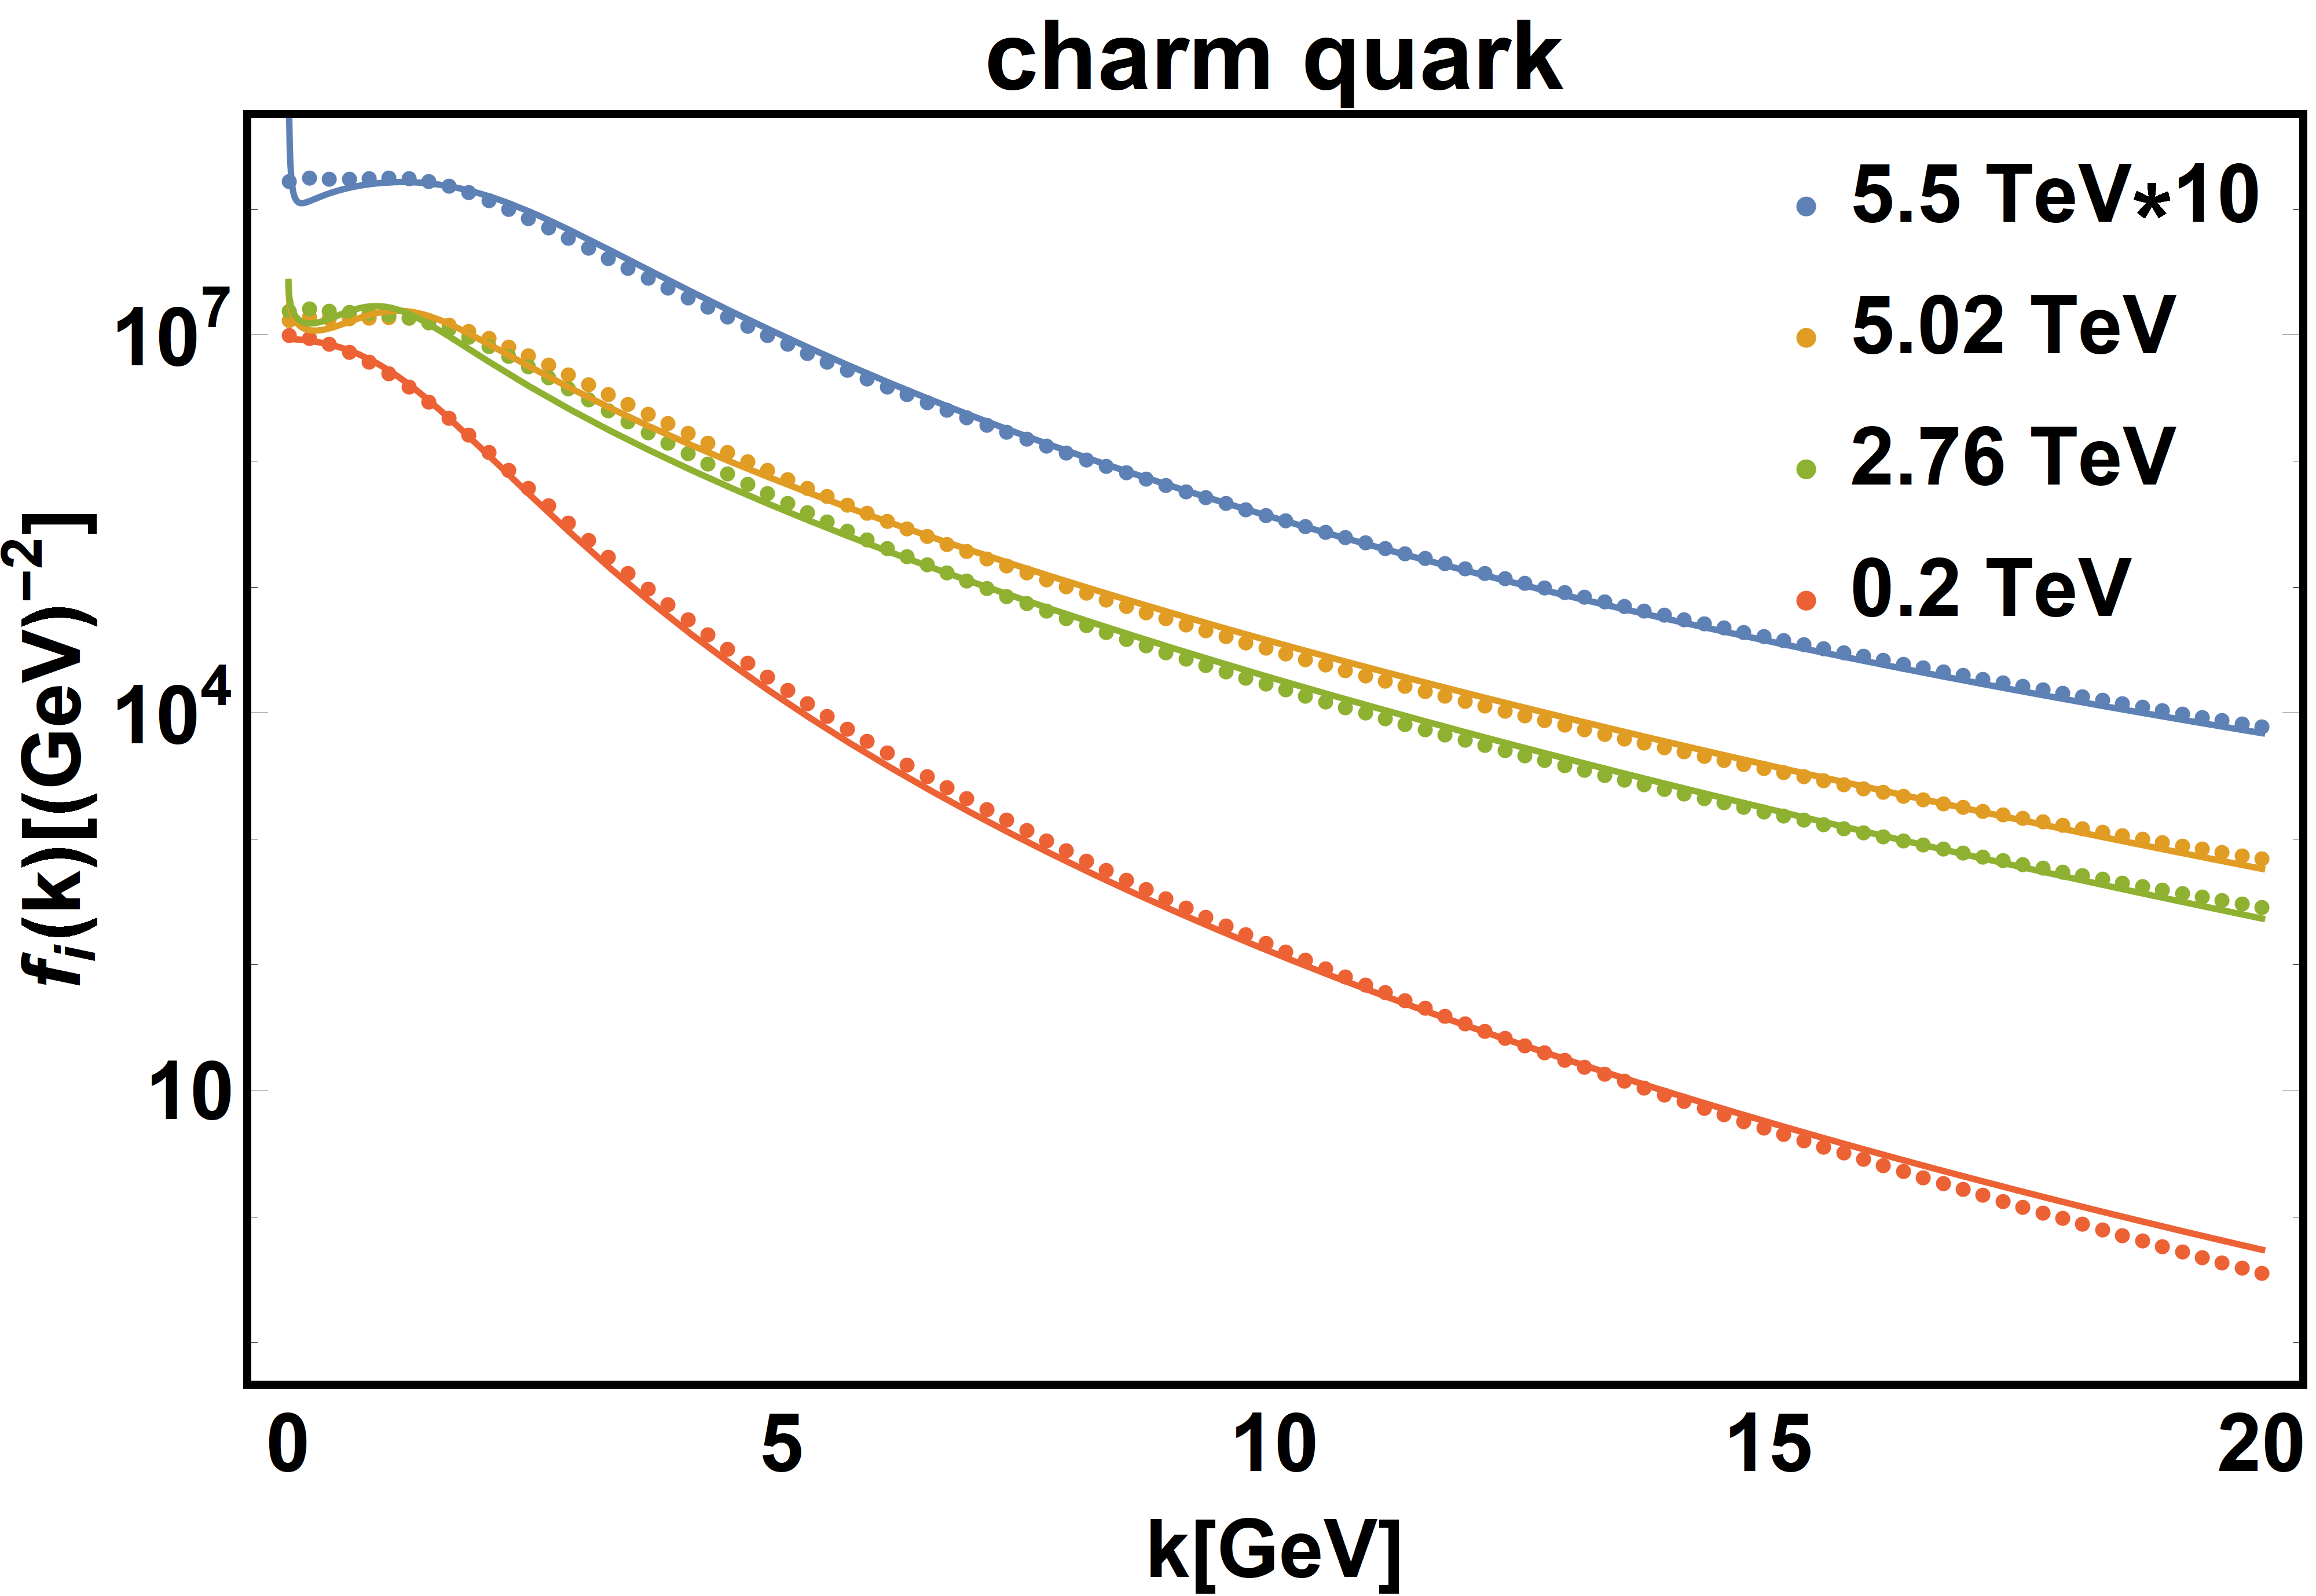
\includegraphics[width=0.45\textwidth]{FONLL_2.png}
	\caption{Charm quark distributions $f_c(k)$ fitted by FONLL data. }
	\label{fig34}
\end{figure}

Besides, compared with v15 $SS(2j)$ component:
 \begin{eqnarray}
	{dN_{J/\psi}^{SS^{2j}} \over p_Tdp_T}={g\Gamma \over p_Tm_T^{J/\psi}}S^c(p_T/2)S^{\bar{c}}(p_T/2),
\end{eqnarray}
our integral limit in Eq.\ref{int_ss2j} actually is consistent with it. After adding QuenchFiqc \ref{QuenchFiqc} and QuenchSPD \ref{QuenchSPD}
 from v15 to our program, we calculated distributions again shown in Fig.\ref{fig35}.
 \begin{eqnarray}
 	c_2(p_2)=1-e^{-(p_2/p_c)^2},\space p_c=0.5 \text{GeV/c}.\label{QuenchSPD}
 \end{eqnarray}
\begin{figure}[H]
	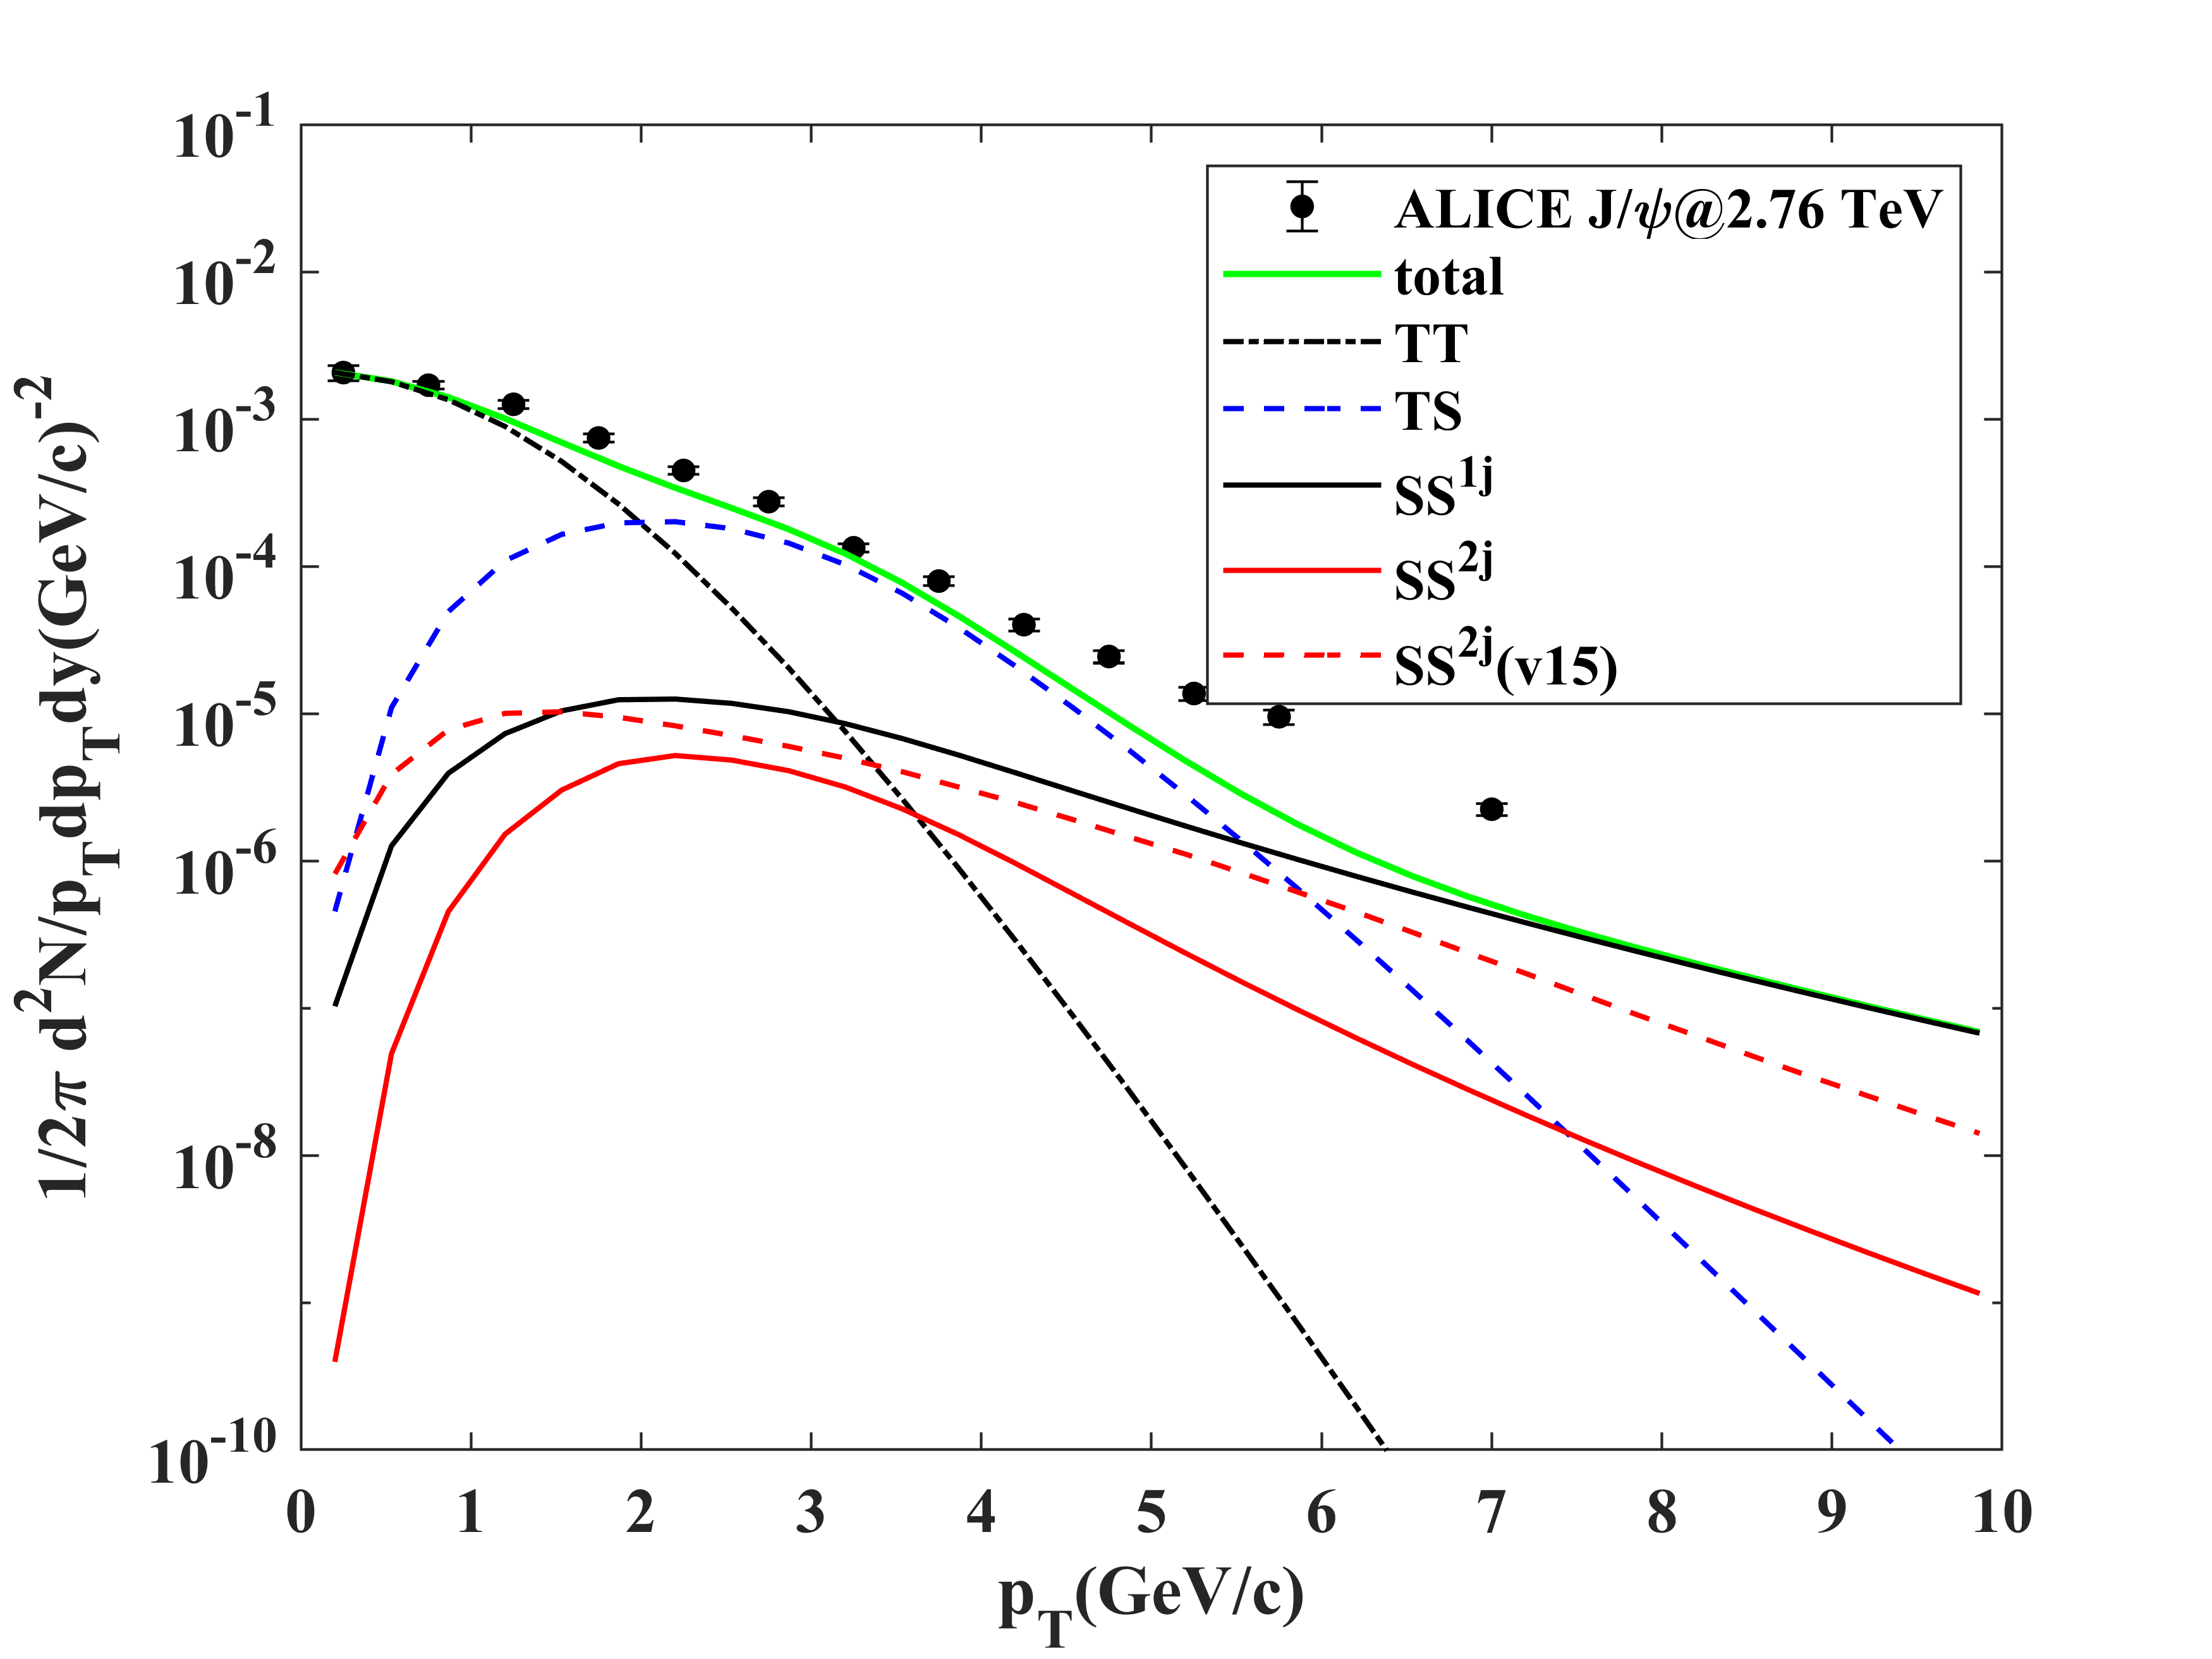
\includegraphics[width=0.45\textwidth]{Jpsi276_compare.png}
	\caption{$J/\psi$ distribution at 2.76 TeV. }
	\label{fig35}
\end{figure}

I should check $SS(1)$ to fit data and $SS(2)$ summing over charm and gluon, while v15 summing over light quark, gluon and charm.

\section{MEETING 2022.12.19}
Last week, as for $SS(2)$ issues, it is found that the difference between two frameworks is minijet distributions. In our(R. Peng) framework, it is easy to write
\begin{eqnarray}
	\frac{dN^{SS(2)}_{J/\psi}}{pdp}&=&\frac{10^{-n}}{p^0p}\sum_{\substack{i=g,c\\ i'=g,c}} \int \frac{dq}{q}\frac{dq'}{q'}F'_i(q)F'_{i'}(q')\nonumber \\
	&&\times  S_i^{\overline c}({p\over 2q})   S_{i'}^c({p\over 2q'}),
\end{eqnarray}
\begin{eqnarray}
	F'_i(q)={1\over \beta L}\int_{q}^{q e^{\beta L}} dkk f_i(k).
\end{eqnarray}
However, in previous RM framework\cite{Zhu_2020}, considering azimuthal angle $\phi$ and impact parameter $b$, much more complex formula is written as
\begin{eqnarray}
	&&F'_i(q)=\int d\xi P_i(\xi,\phi,b) \int dkk f_i(k)G(k,q,\xi),\\
	&&G(k,q,\xi)=q\delta(q-ke^{-\xi}),\\
	&&\gamma_g(g)=\frac{\gamma_0}{1+(q/q_0)^2},\\
	&&\gamma_0=2.8,q_0=7,\text{  PbPb@2.76}.
\end{eqnarray}
Thus, in two framework, there are parameters $\gamma_0$, $q_0$ or $\beta L$ to fit respectively. It is difficult to compare them owing to no right reference. While transferring code from v15 to ours, it is verified that shower parton distribution $S_i^j$ is much larger than ours. Next we determine $SS(1)$ first to ensure minijet distribution, in which v15 used different method for calculation.

As a result, calculation of $SS(2)$ adopted process in v15, except for $S_i^j$. All are shown in Fig.\ref{fig36}. 

\begin{figure}[H]
	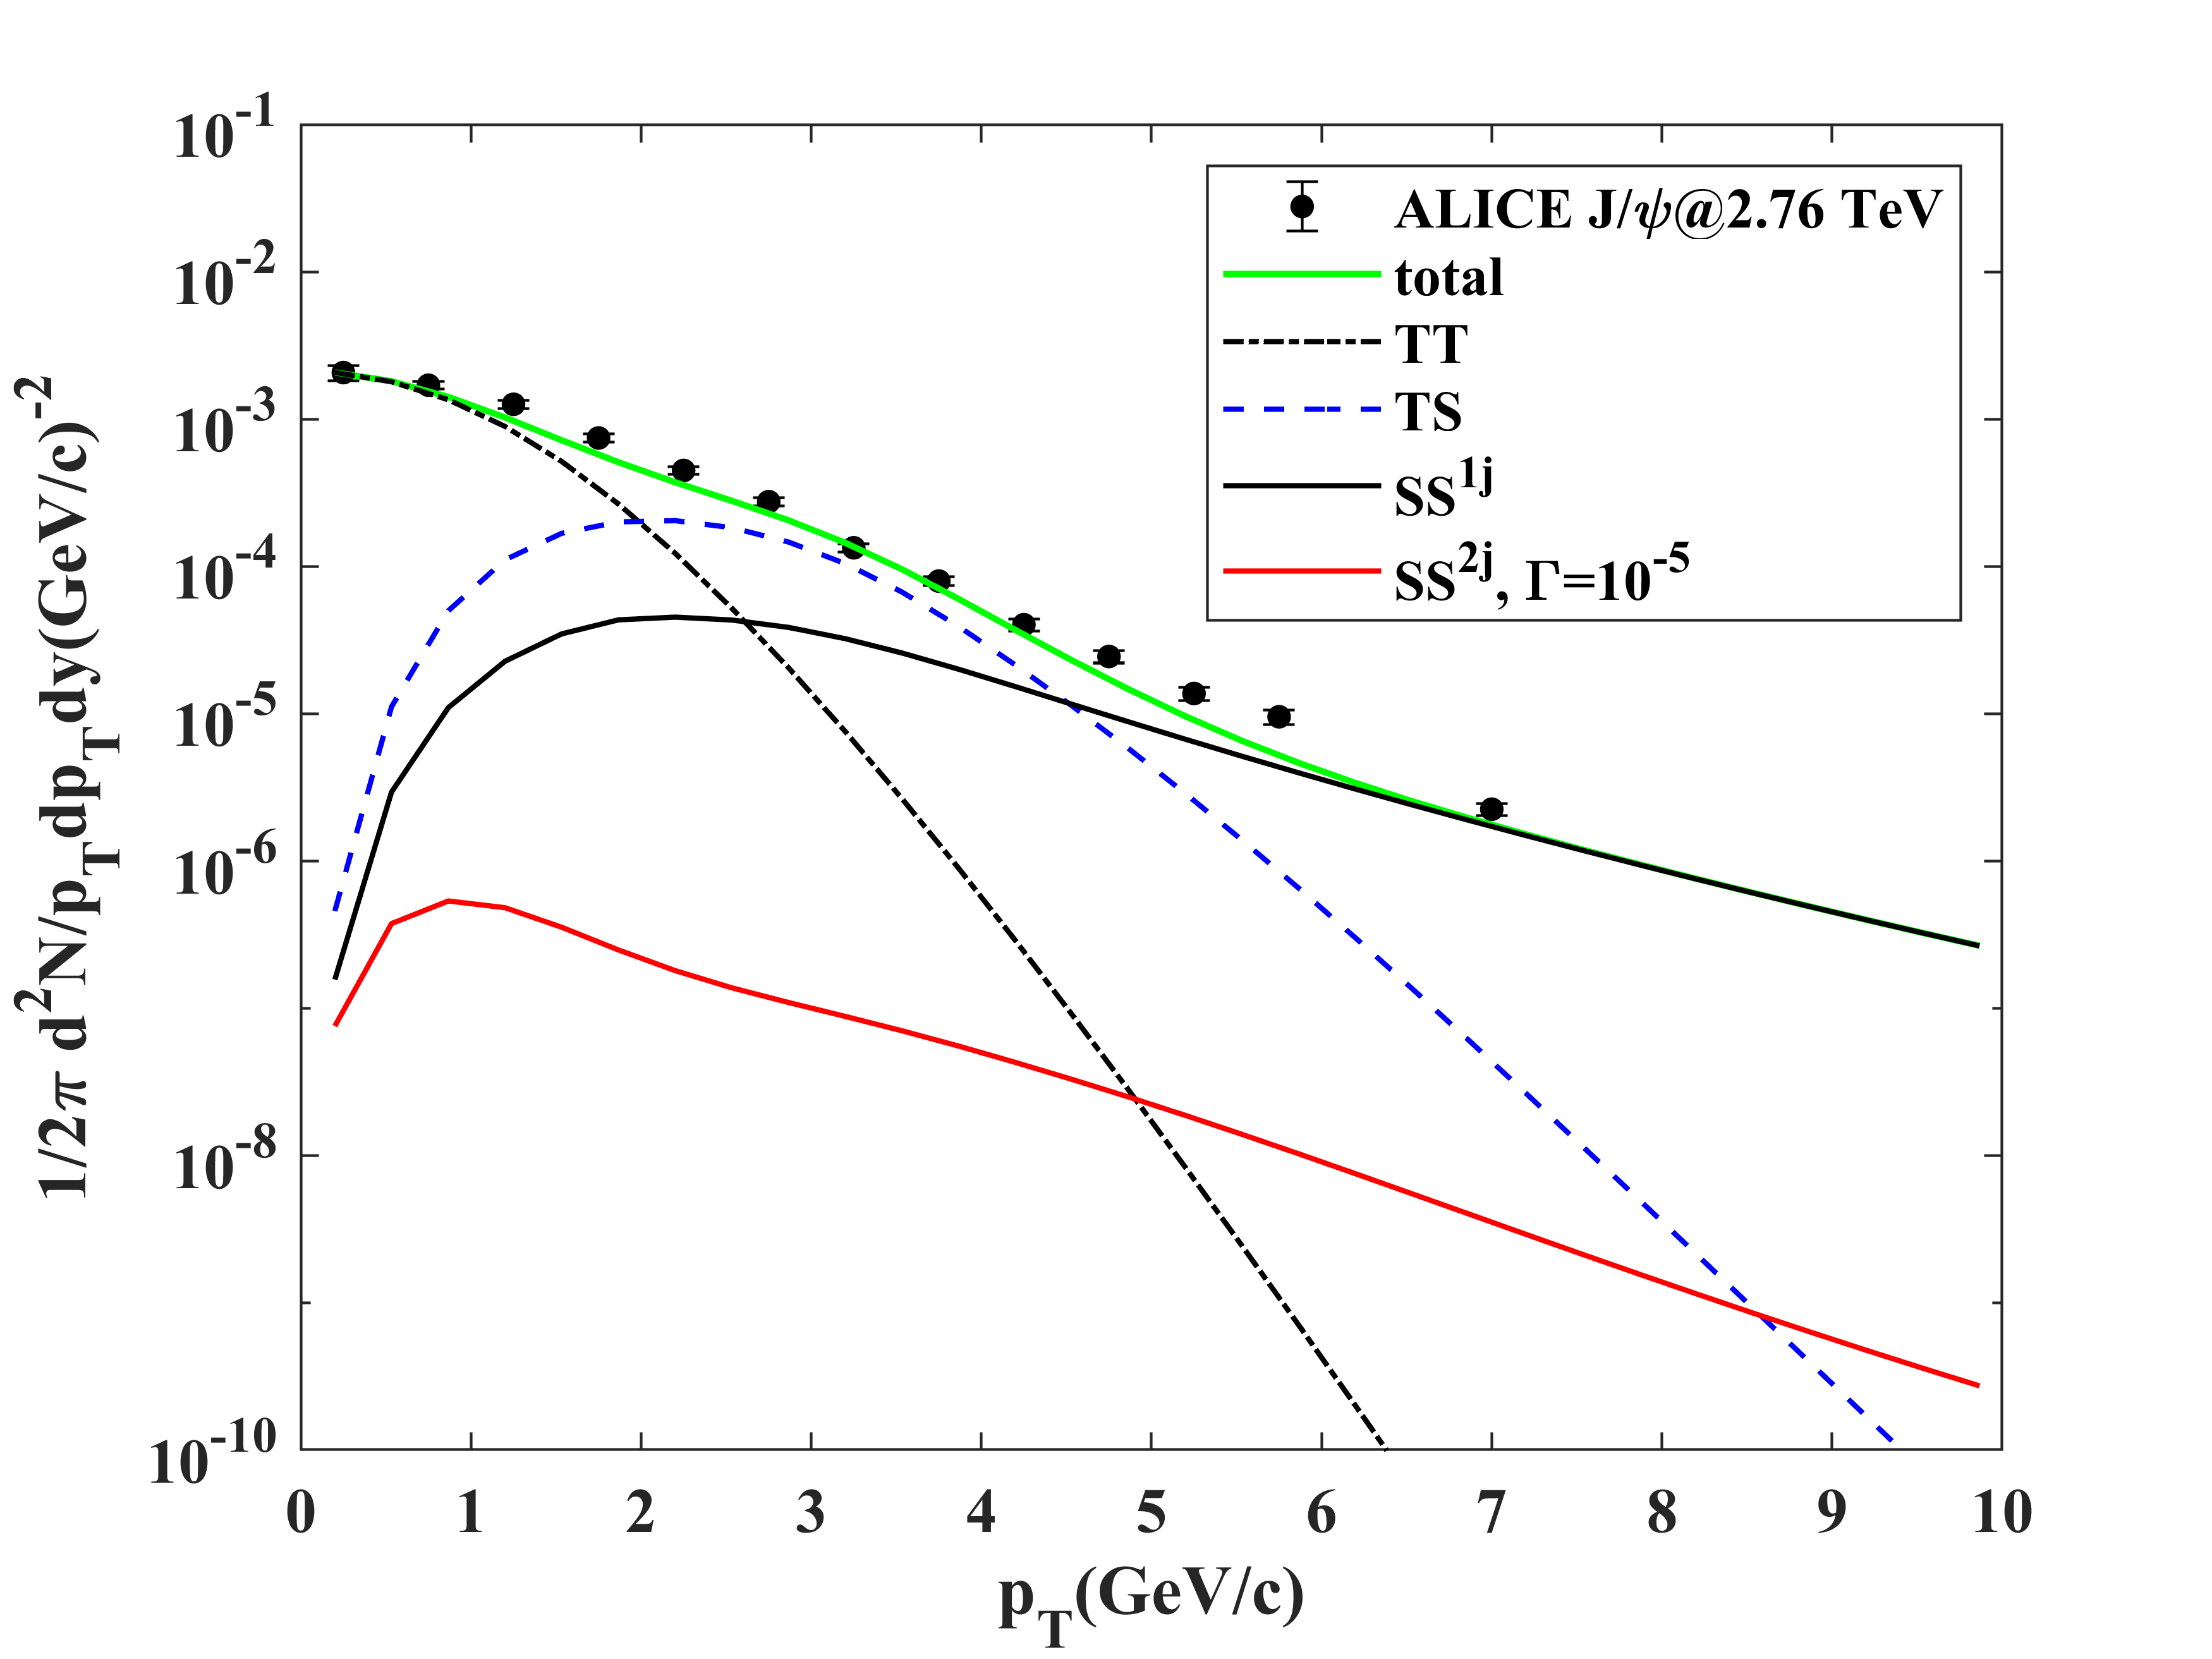
\includegraphics[width=0.45\textwidth]{Jpsi276_221218.png}
	\caption{$J/\psi$ distribution at 2.76 TeV. }
	\label{fig36}
\end{figure}

We should figure out the bug in calculation of $SS(2)$.

\section{MEETING 2023.01.02}
Last week, the bug in $SS(2)$ was found, which is a wrong order in a loop, resulting in much larger results in $SS(2)$. After modifying, new spectrum is shown in Fig.\ref{fig37}.
\begin{figure}[H]
	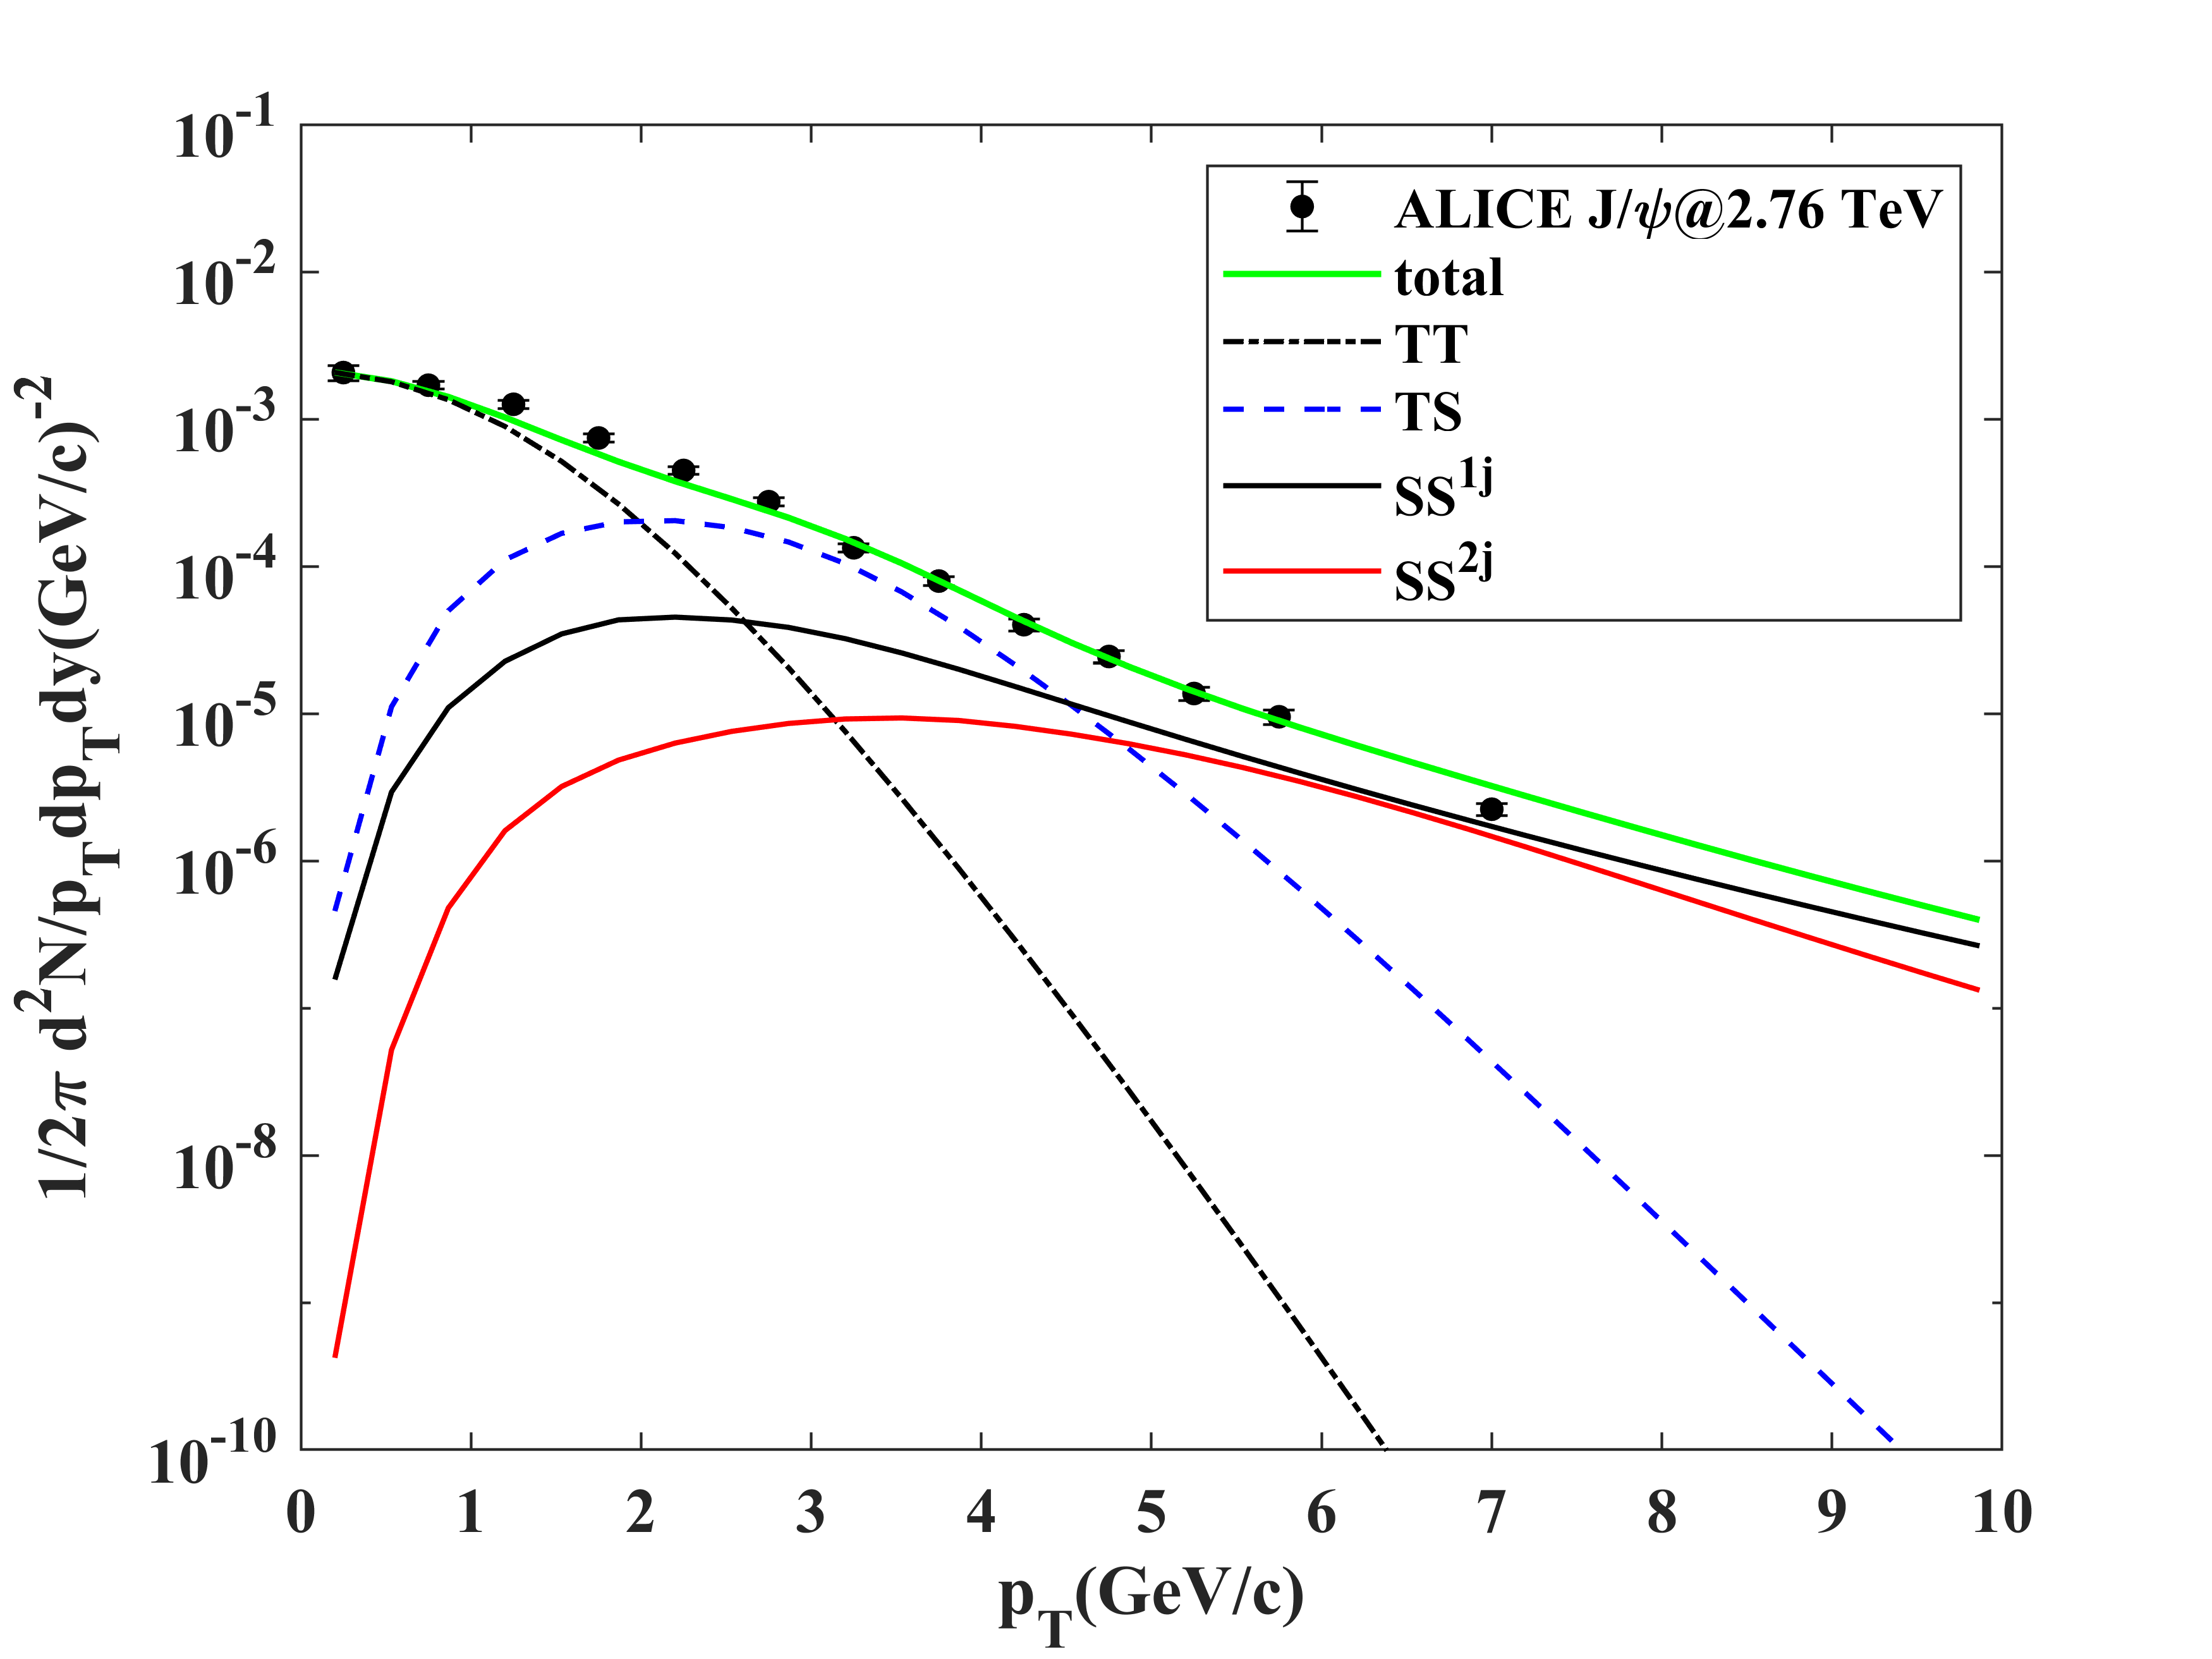
\includegraphics[width=0.45\textwidth]{Jpsi276_230101.png}
	\caption{$J/\psi$ distribution at 2.76 TeV with $\Gamma=10^{-2}$. }
	\label{fig37}
\end{figure}
Next, I will check all the code and reproduce others.

\section{MEETING 2023.01.09}
After refactoring the code, the first results are shown below. And next parameters should be fitted to be consistent with experiments.
\begin{figure}[H]
	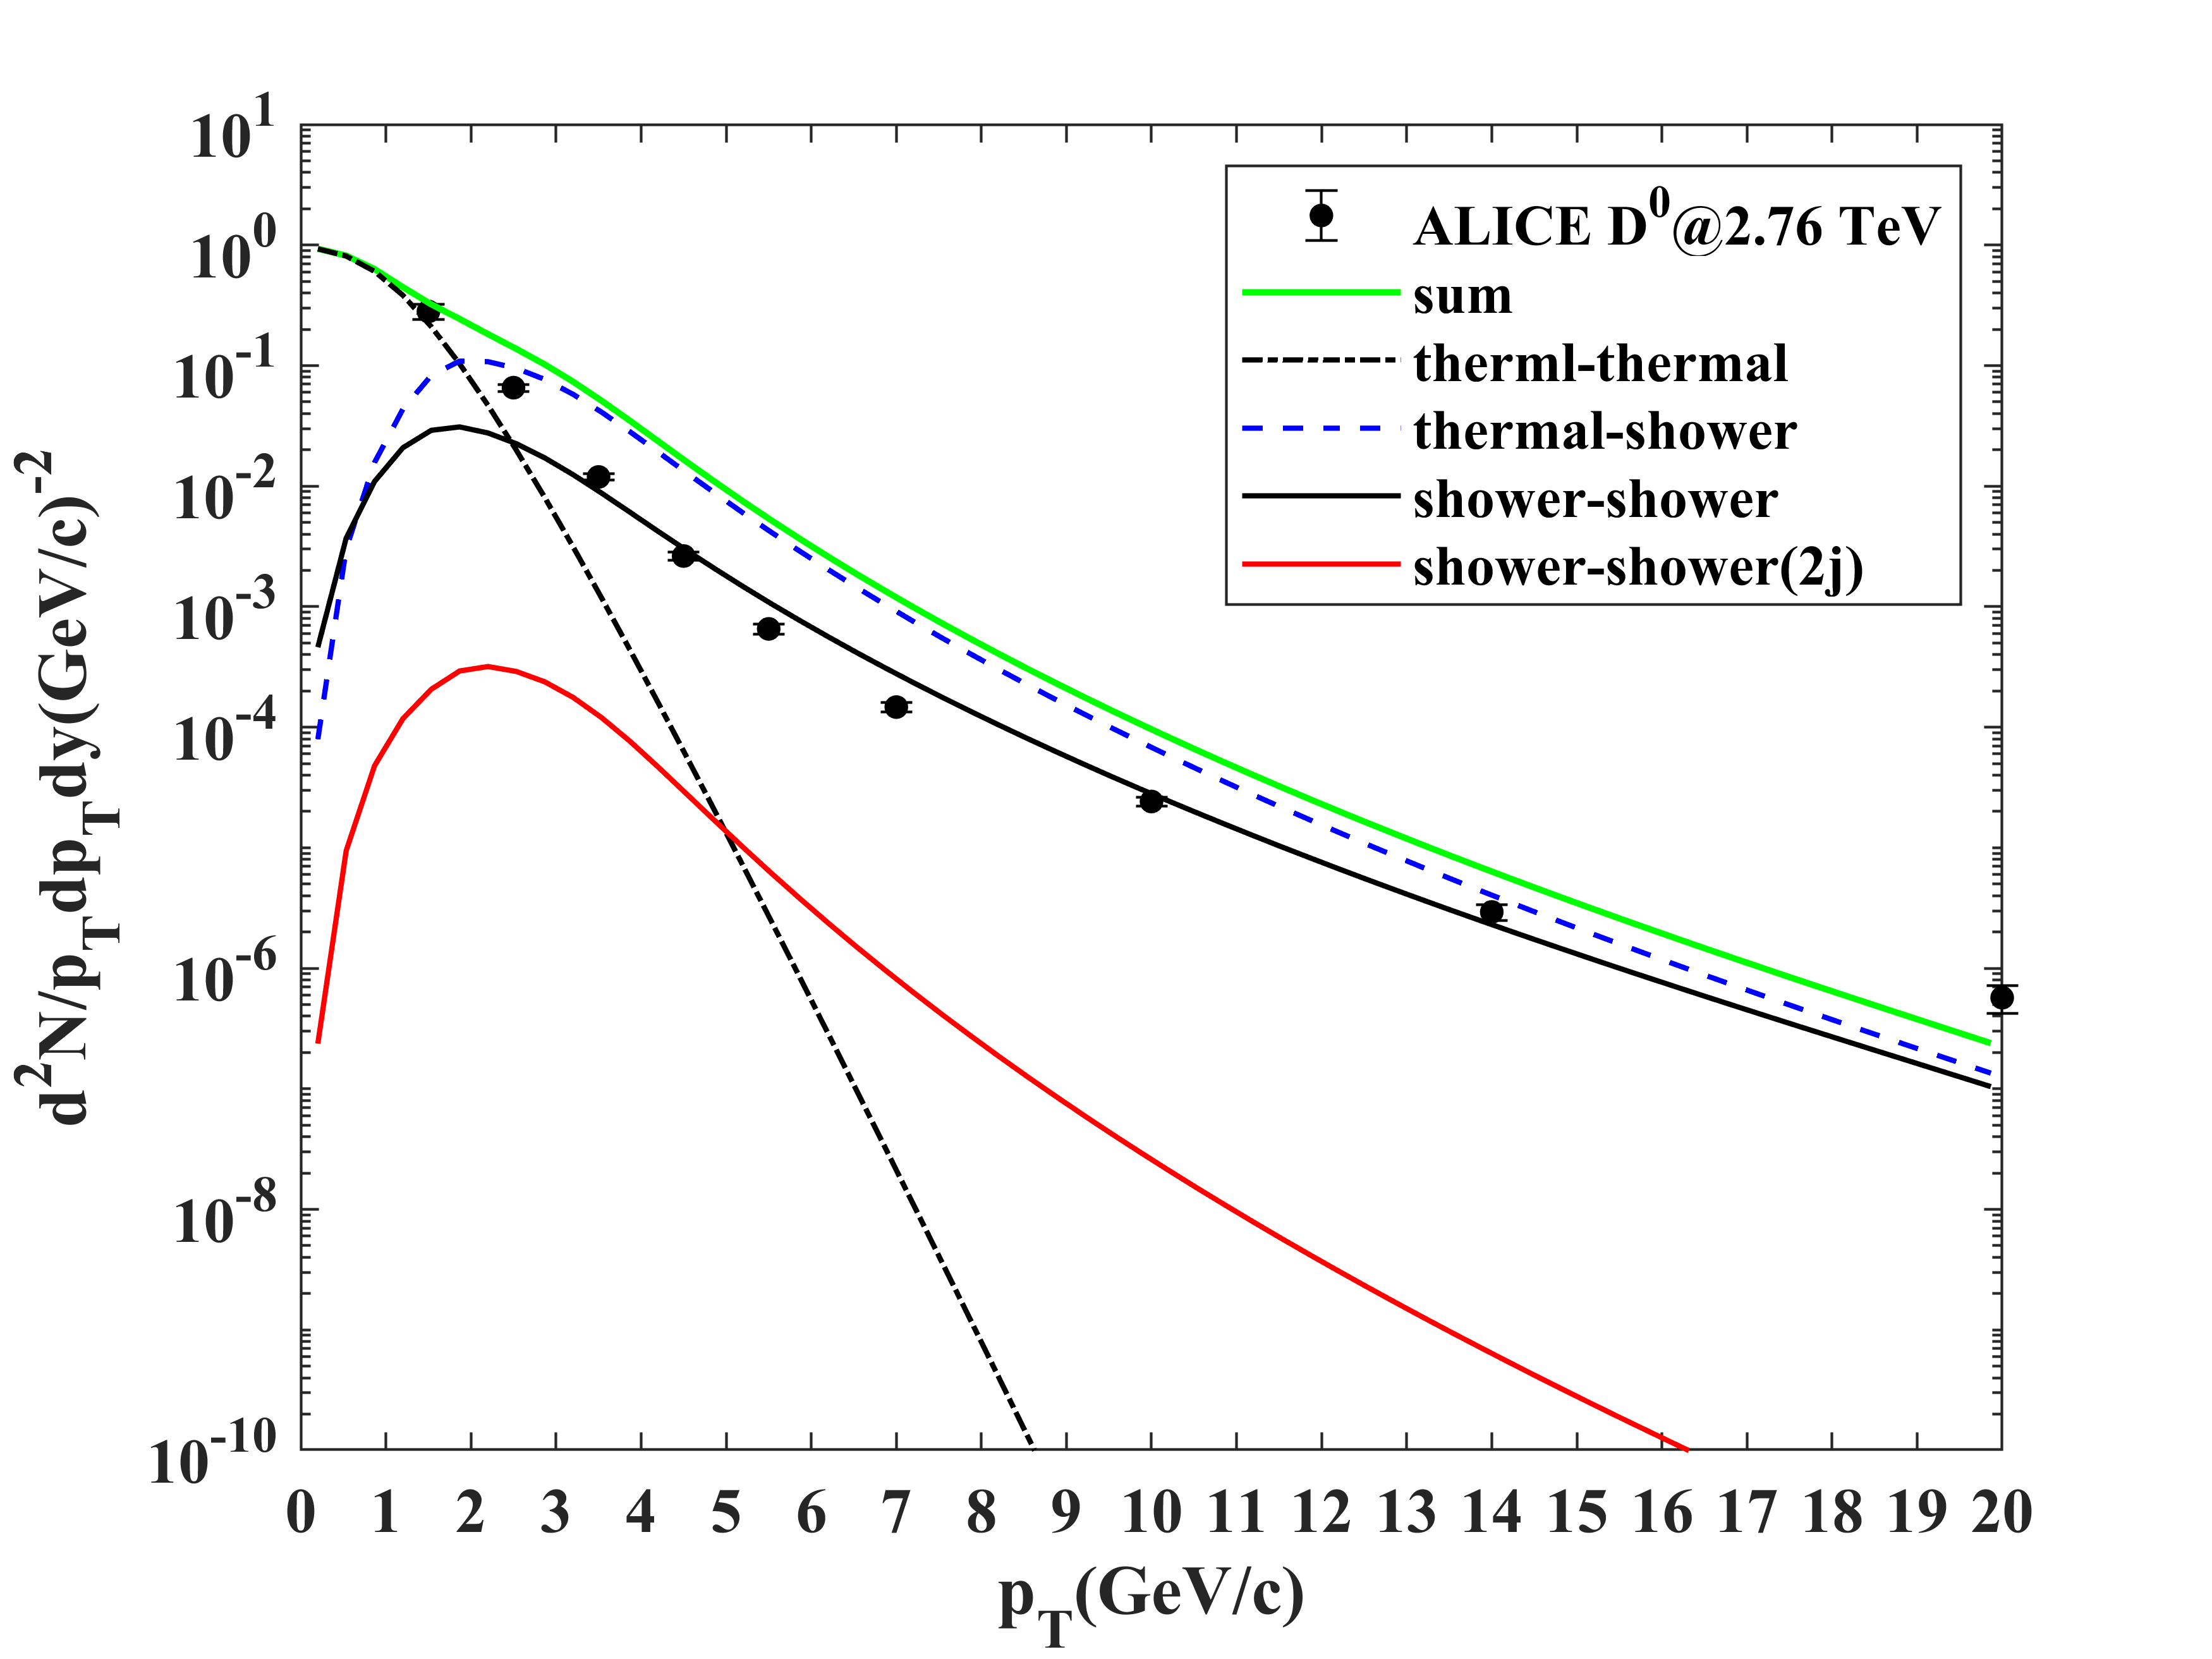
\includegraphics[width=0.45\textwidth]{D0276_230109.png}
	\caption{$D^0$ distribution at 2.76 TeV with $\Gamma=10^{-2}$. }
	\label{fig38}
\end{figure}
\begin{figure}[H]
	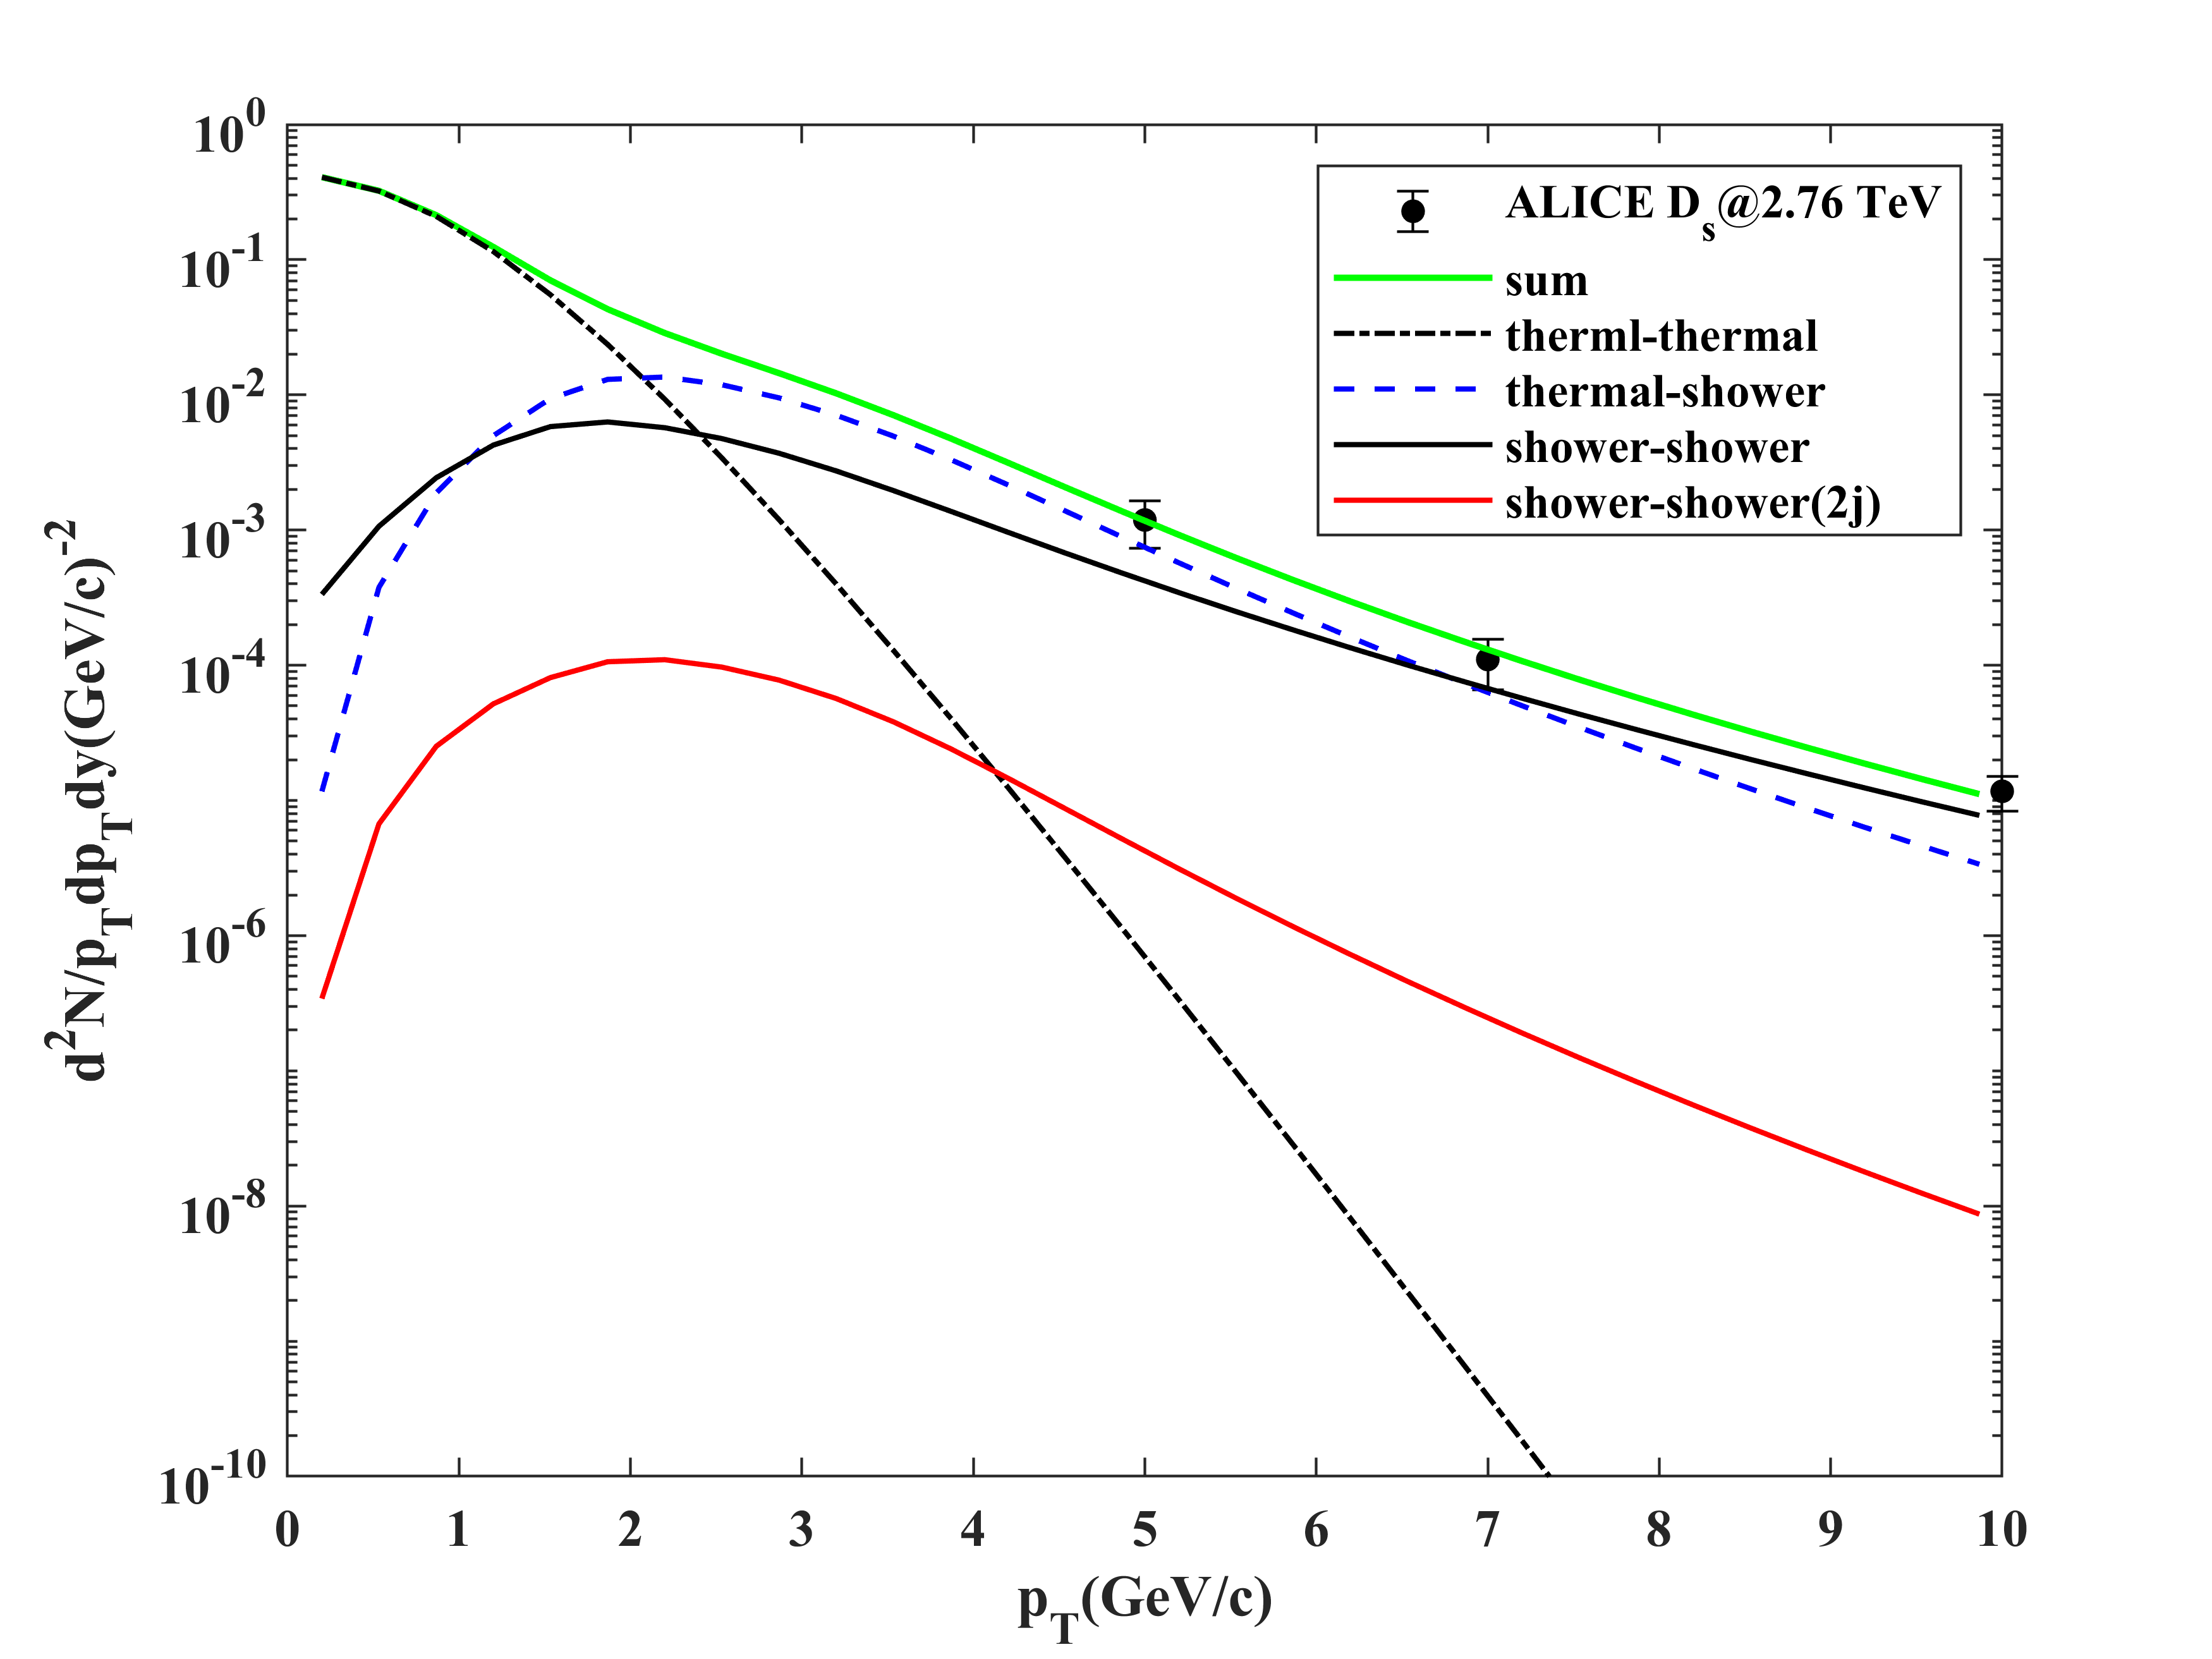
\includegraphics[width=0.45\textwidth]{Ds276_230109.png}
	\caption{$D_s$ distribution at 2.76 TeV with $\Gamma=10^{-2}$. }
	\label{fig39}
\end{figure}
\begin{figure}[H]
	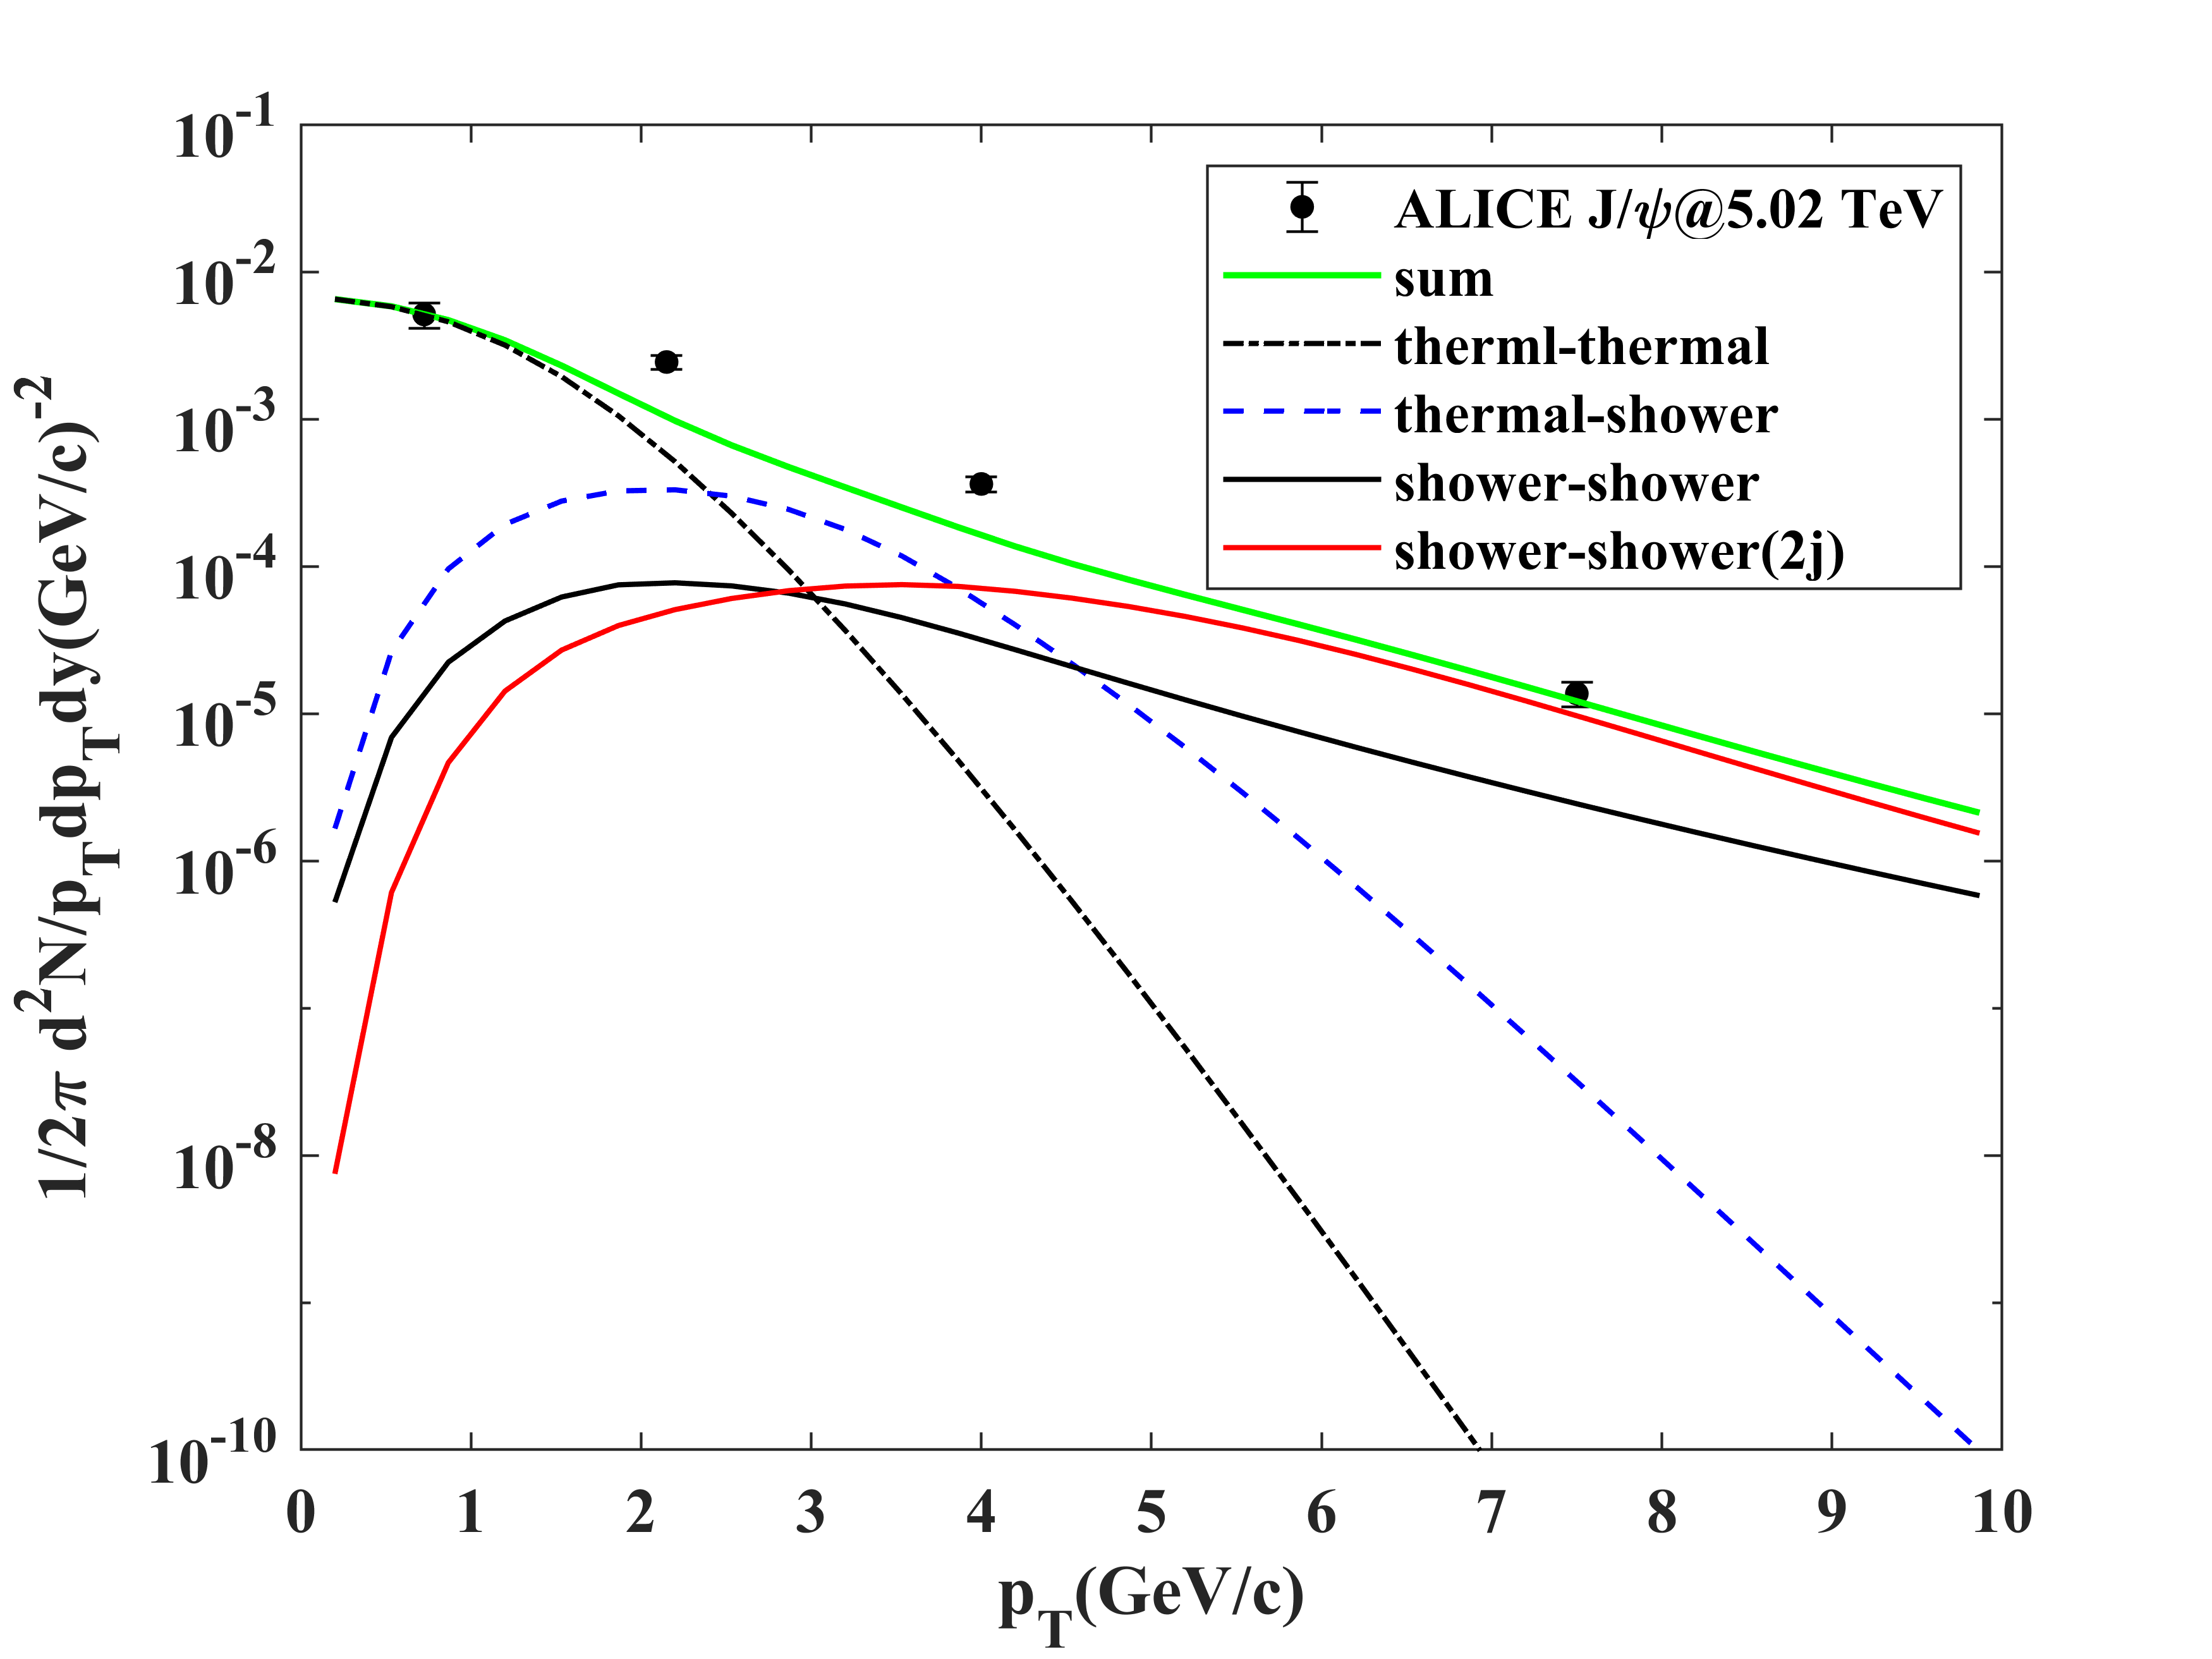
\includegraphics[width=0.45\textwidth]{Jpsi502_230109.png}
	\caption{$J/\psi$ distribution at 5.02 TeV with $\Gamma=10^{-2}$. }
	\label{fig40}
\end{figure}
\begin{figure}[H]
	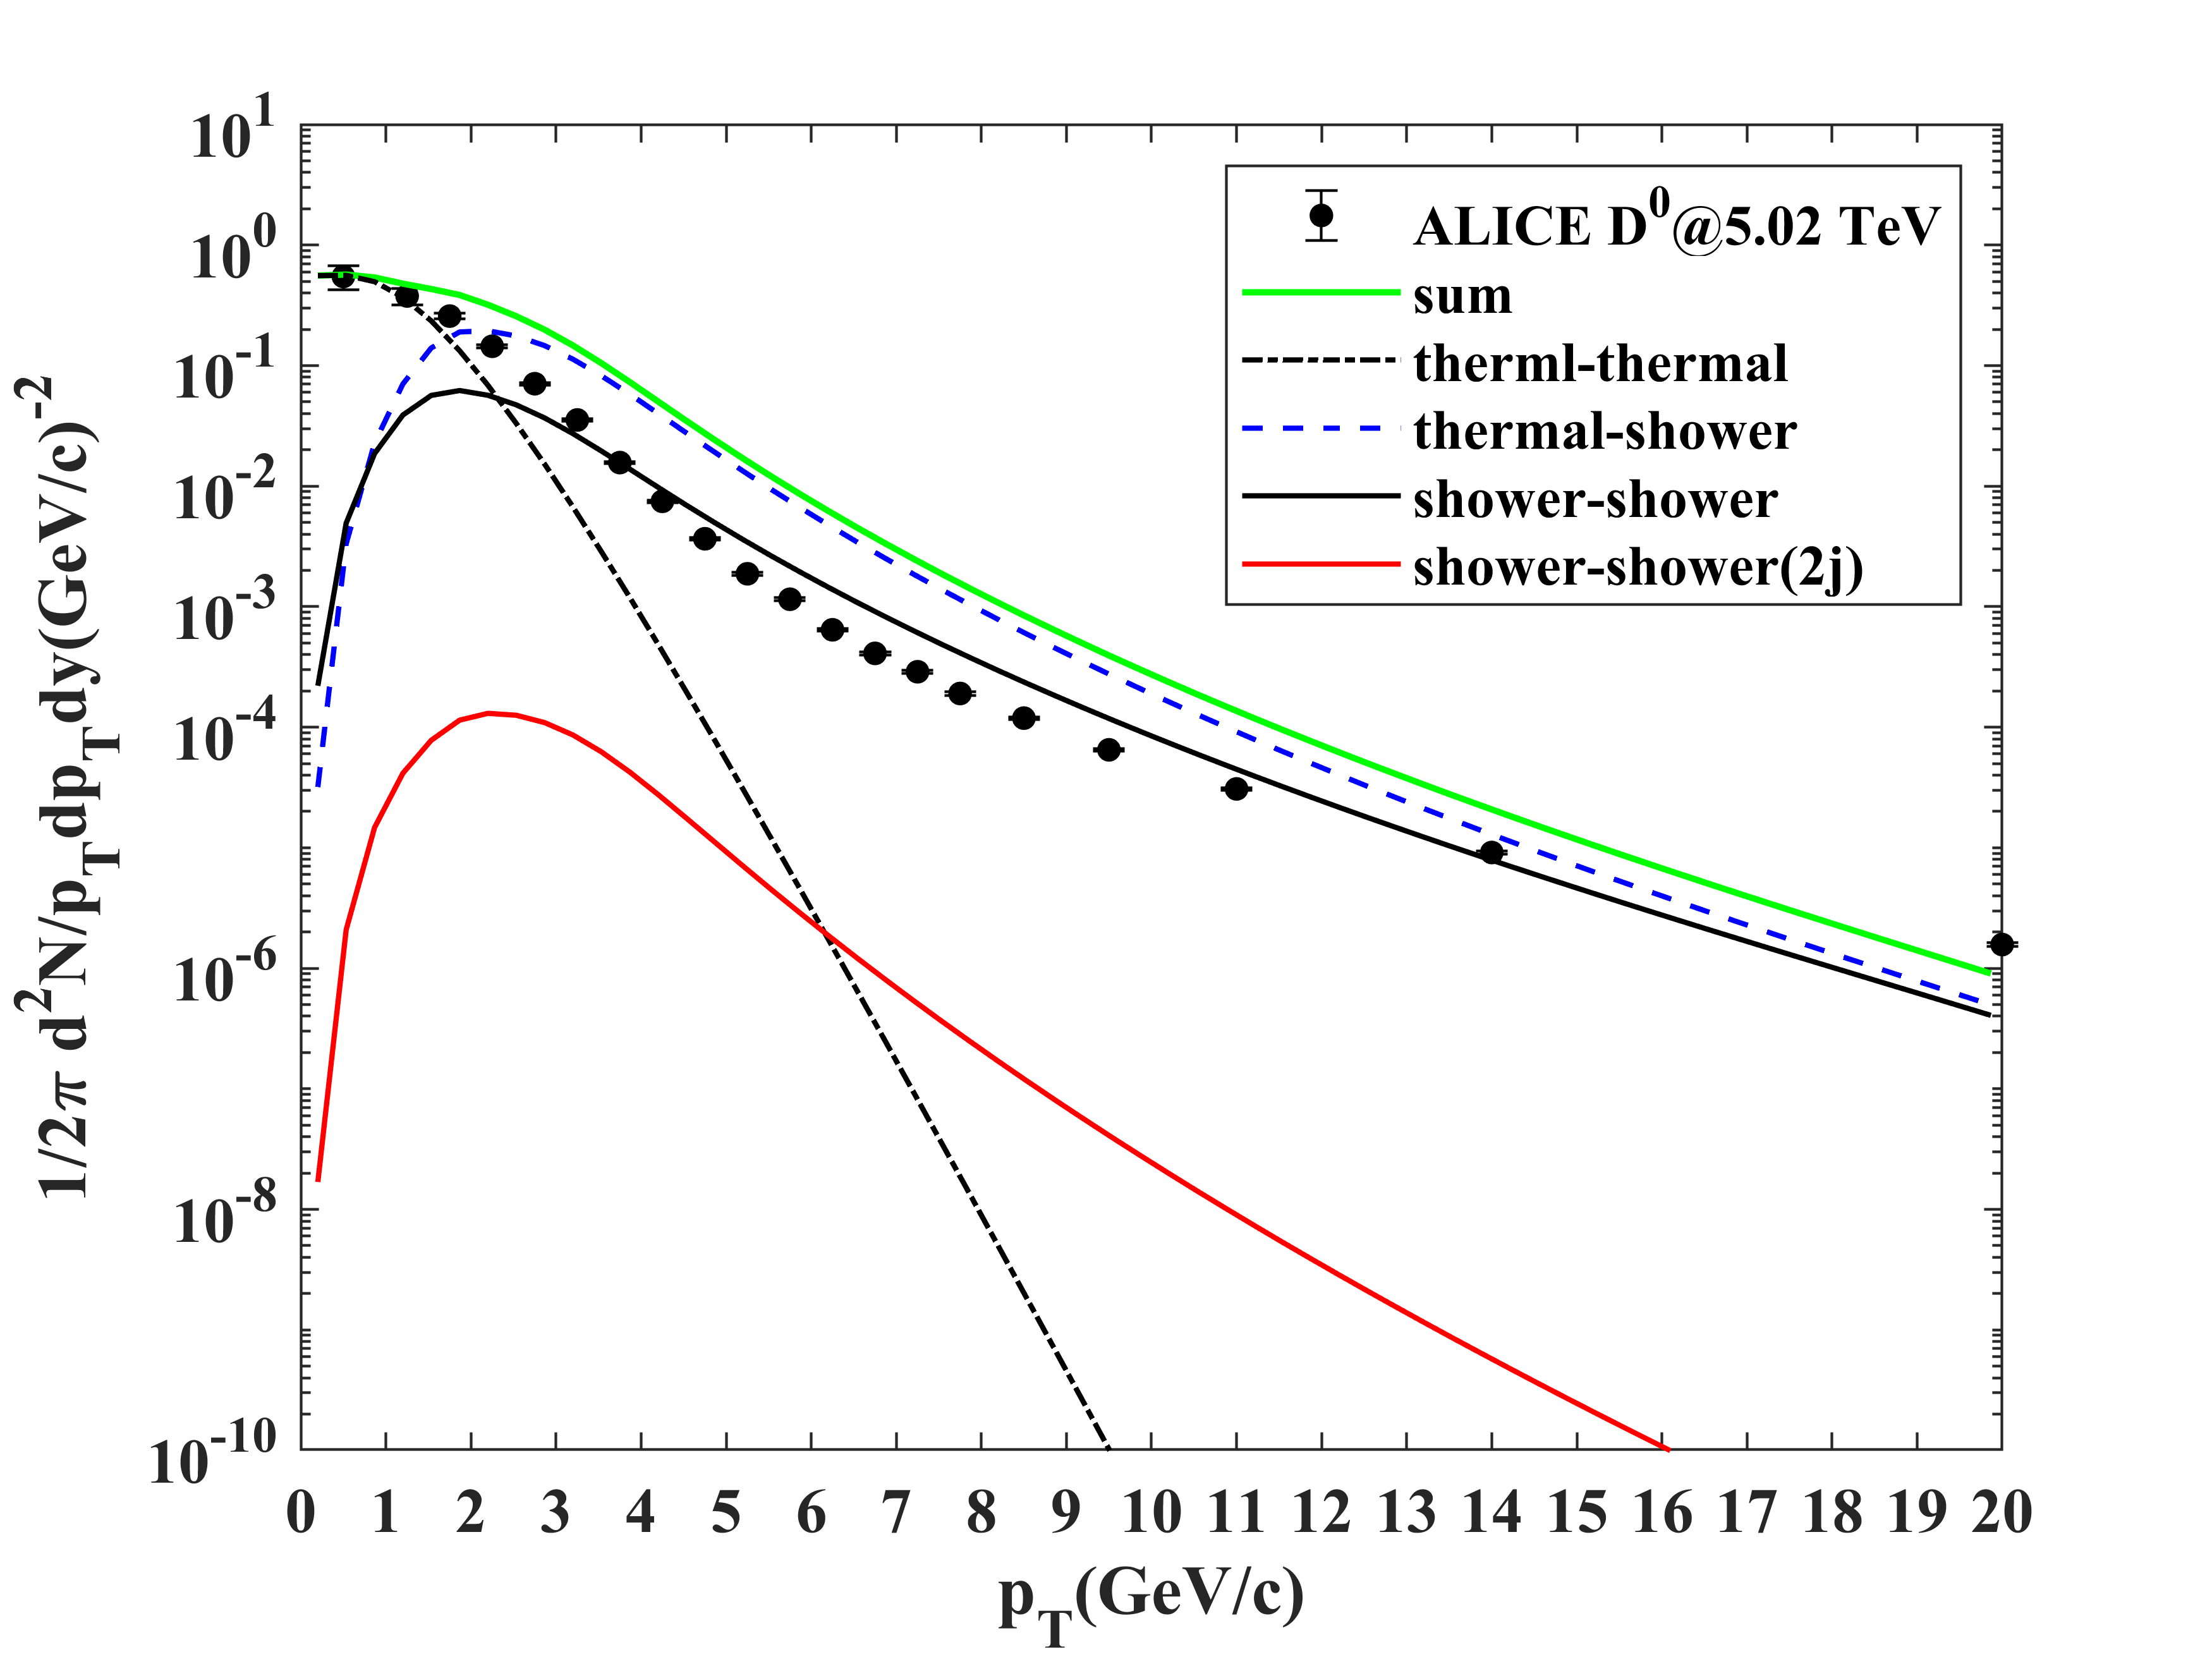
\includegraphics[width=0.45\textwidth]{D0502_230109.png}
	\caption{$D^0$ distribution at 5.02 TeV with $\Gamma=10^{-2}$. }
	\label{fig41}
\end{figure}
\begin{figure}[H]
	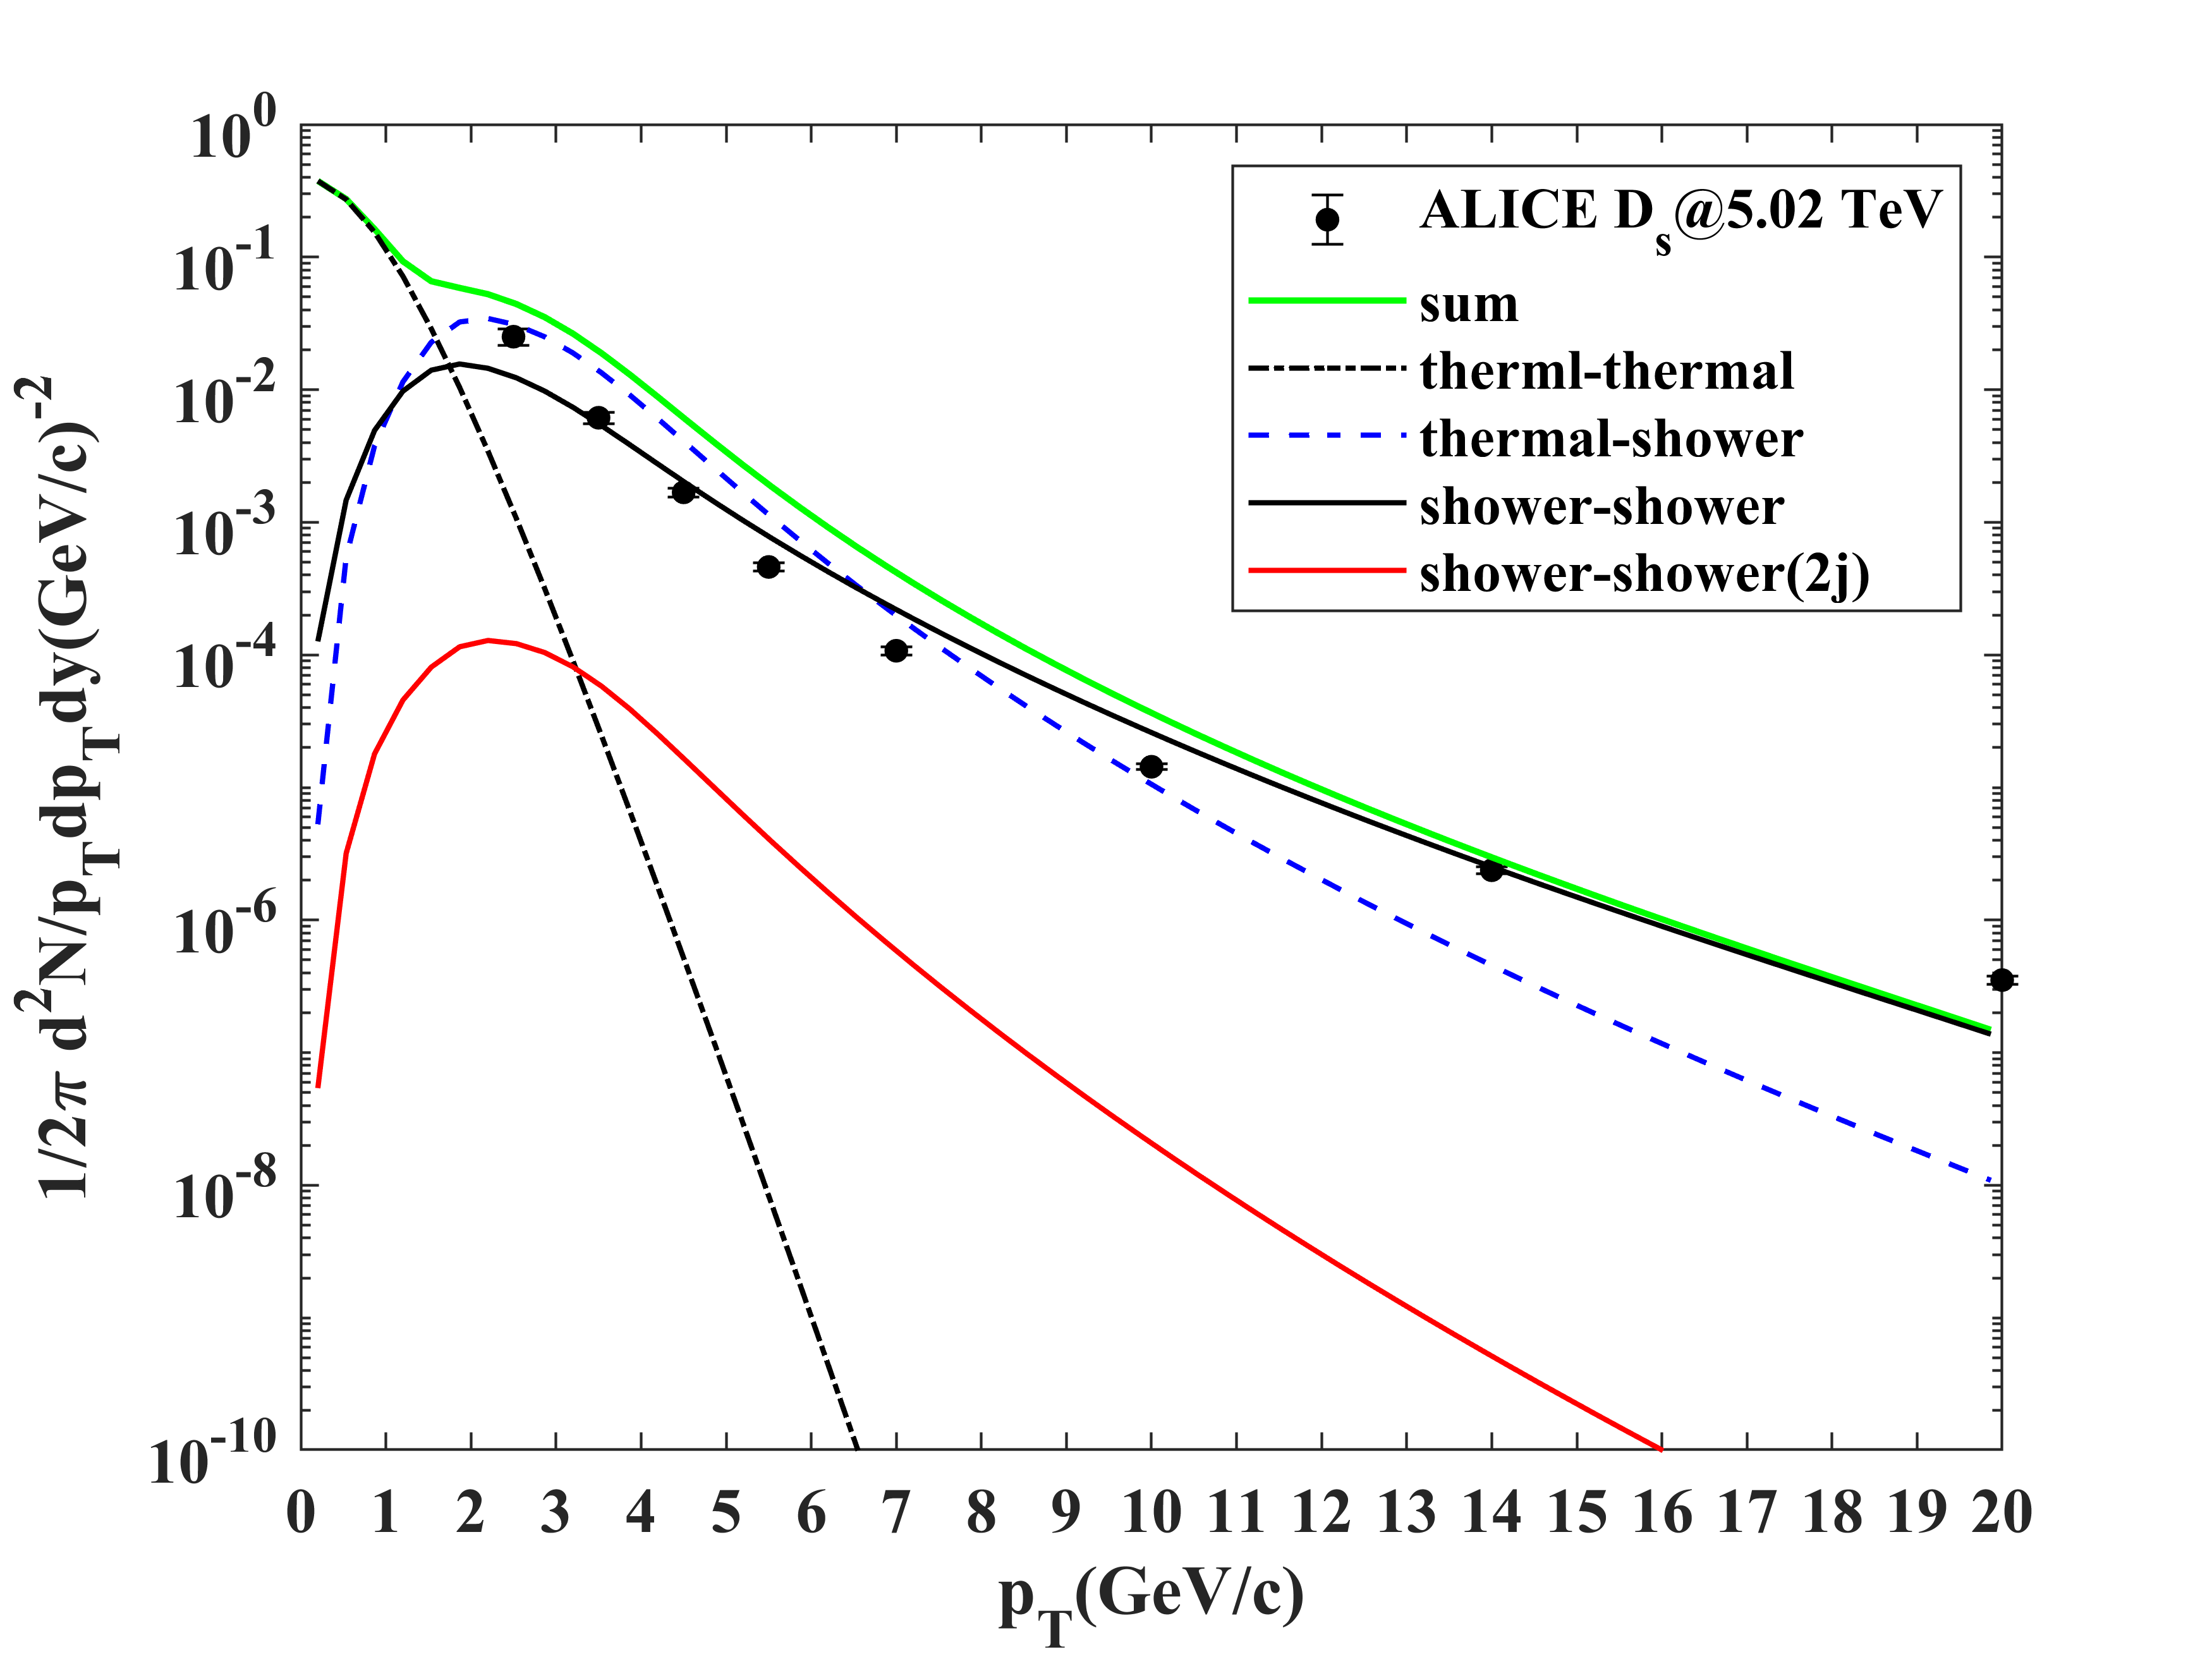
\includegraphics[width=0.45\textwidth]{Ds502_230109.png}
	\caption{$D_s$ distribution at 5.02 TeV with $\Gamma=10^{-2}$. }
	\label{fig42}
\end{figure}
It is suggested that we should replace all the integral algorithm with exponential integral algorithm in v15 program, owing to the scale of integrand.

\section{MEETING 2023.01.30}
While adding exponential integral algorithm in v15 program, we find it difficult to reproduce spectrum using old parameters in v15 (the step fdel=0.02, 0.05, 0.1). Thus this issue is tackled after decreasing the step to 0.01/0.005, however, increasing the computing cost, so that now we can reproduce spectrum for $J/\psi$ and $D^0$ at 2.76 TeV at least.

It is suggested to check the accuracy of integral algorithms. Then we will fit the spectrum.

\section{MEETING 2023.02.06}
After checking the accuracy of integral algorithms, it is found that the step 0.01 is suitable for our calculation. Then we fit the spectrum, shown below.
\begin{figure}[H]
	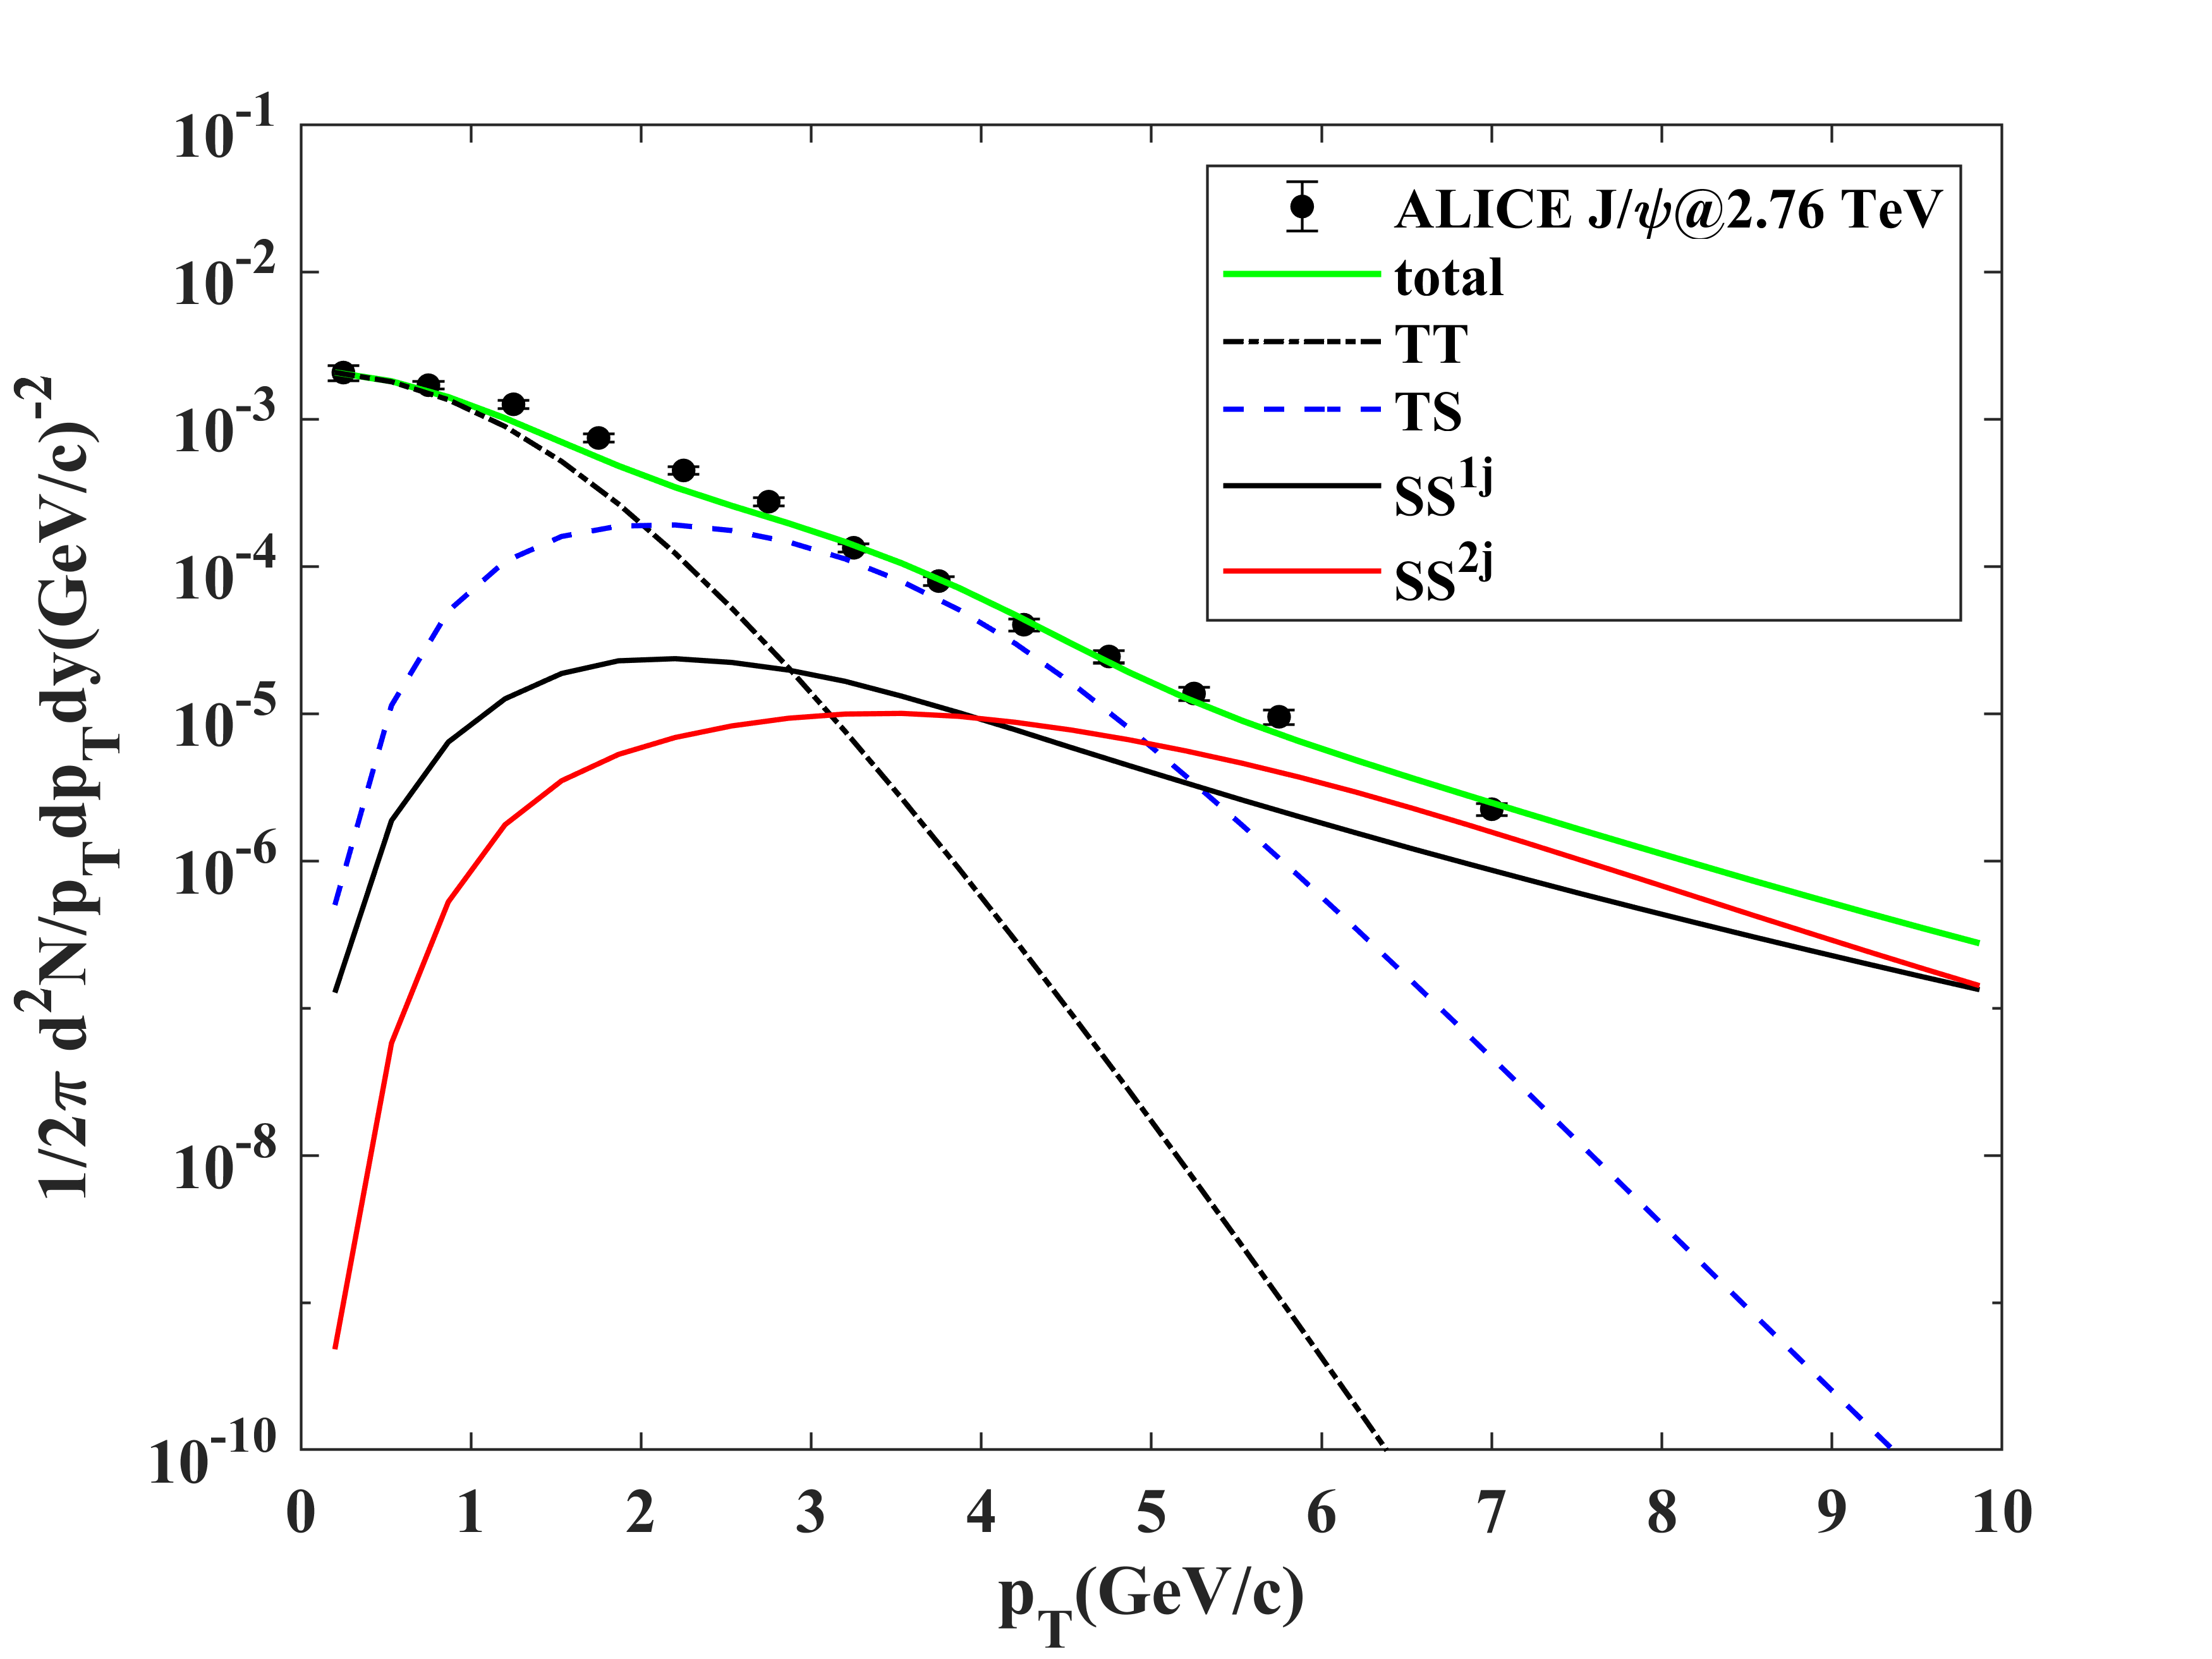
\includegraphics[width=0.45\textwidth]{Jpsi276_230205.png}
	\caption{$J/\psi$ distribution at 2.76 TeV with $\Gamma=10^{-2}$. }
	\label{fig43}
\end{figure}
\begin{figure}[H]
	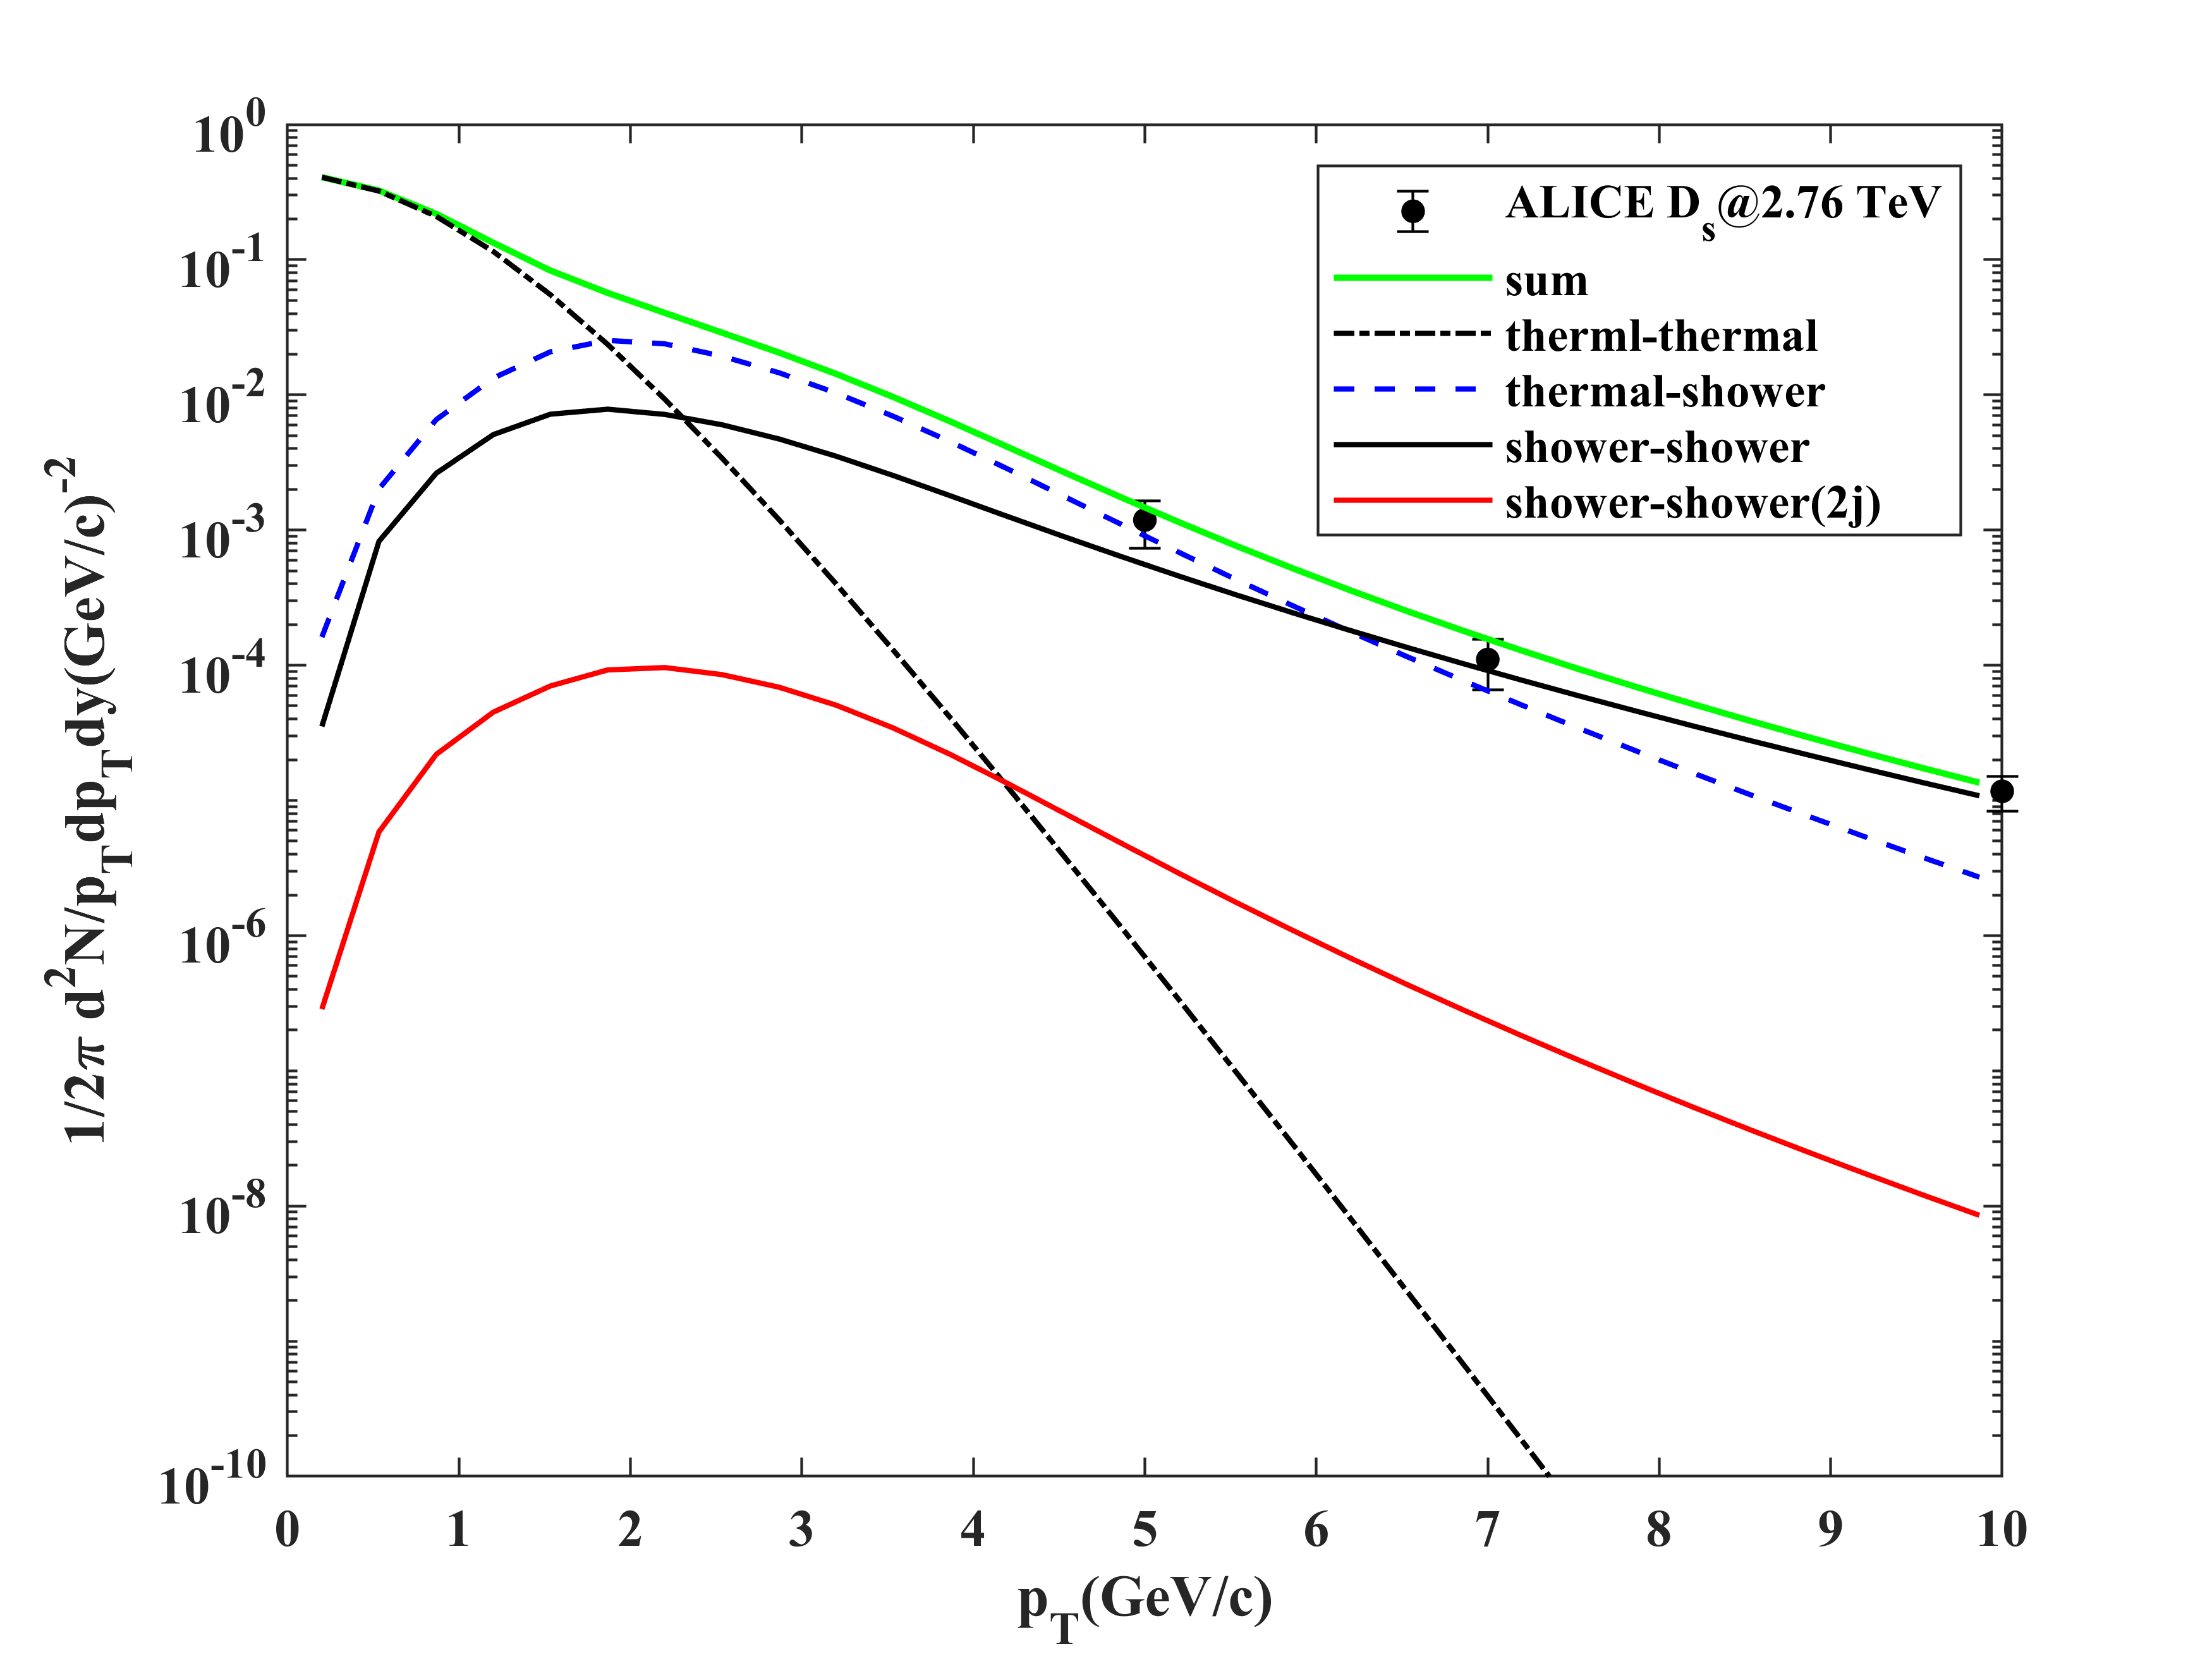
\includegraphics[width=0.45\textwidth]{Ds276_230205.png}
	\caption{$D_s$ distribution at 2.76 TeV with $\Gamma=10^{-2}$. }
	\label{fig44}
\end{figure}
\begin{figure}[H]
	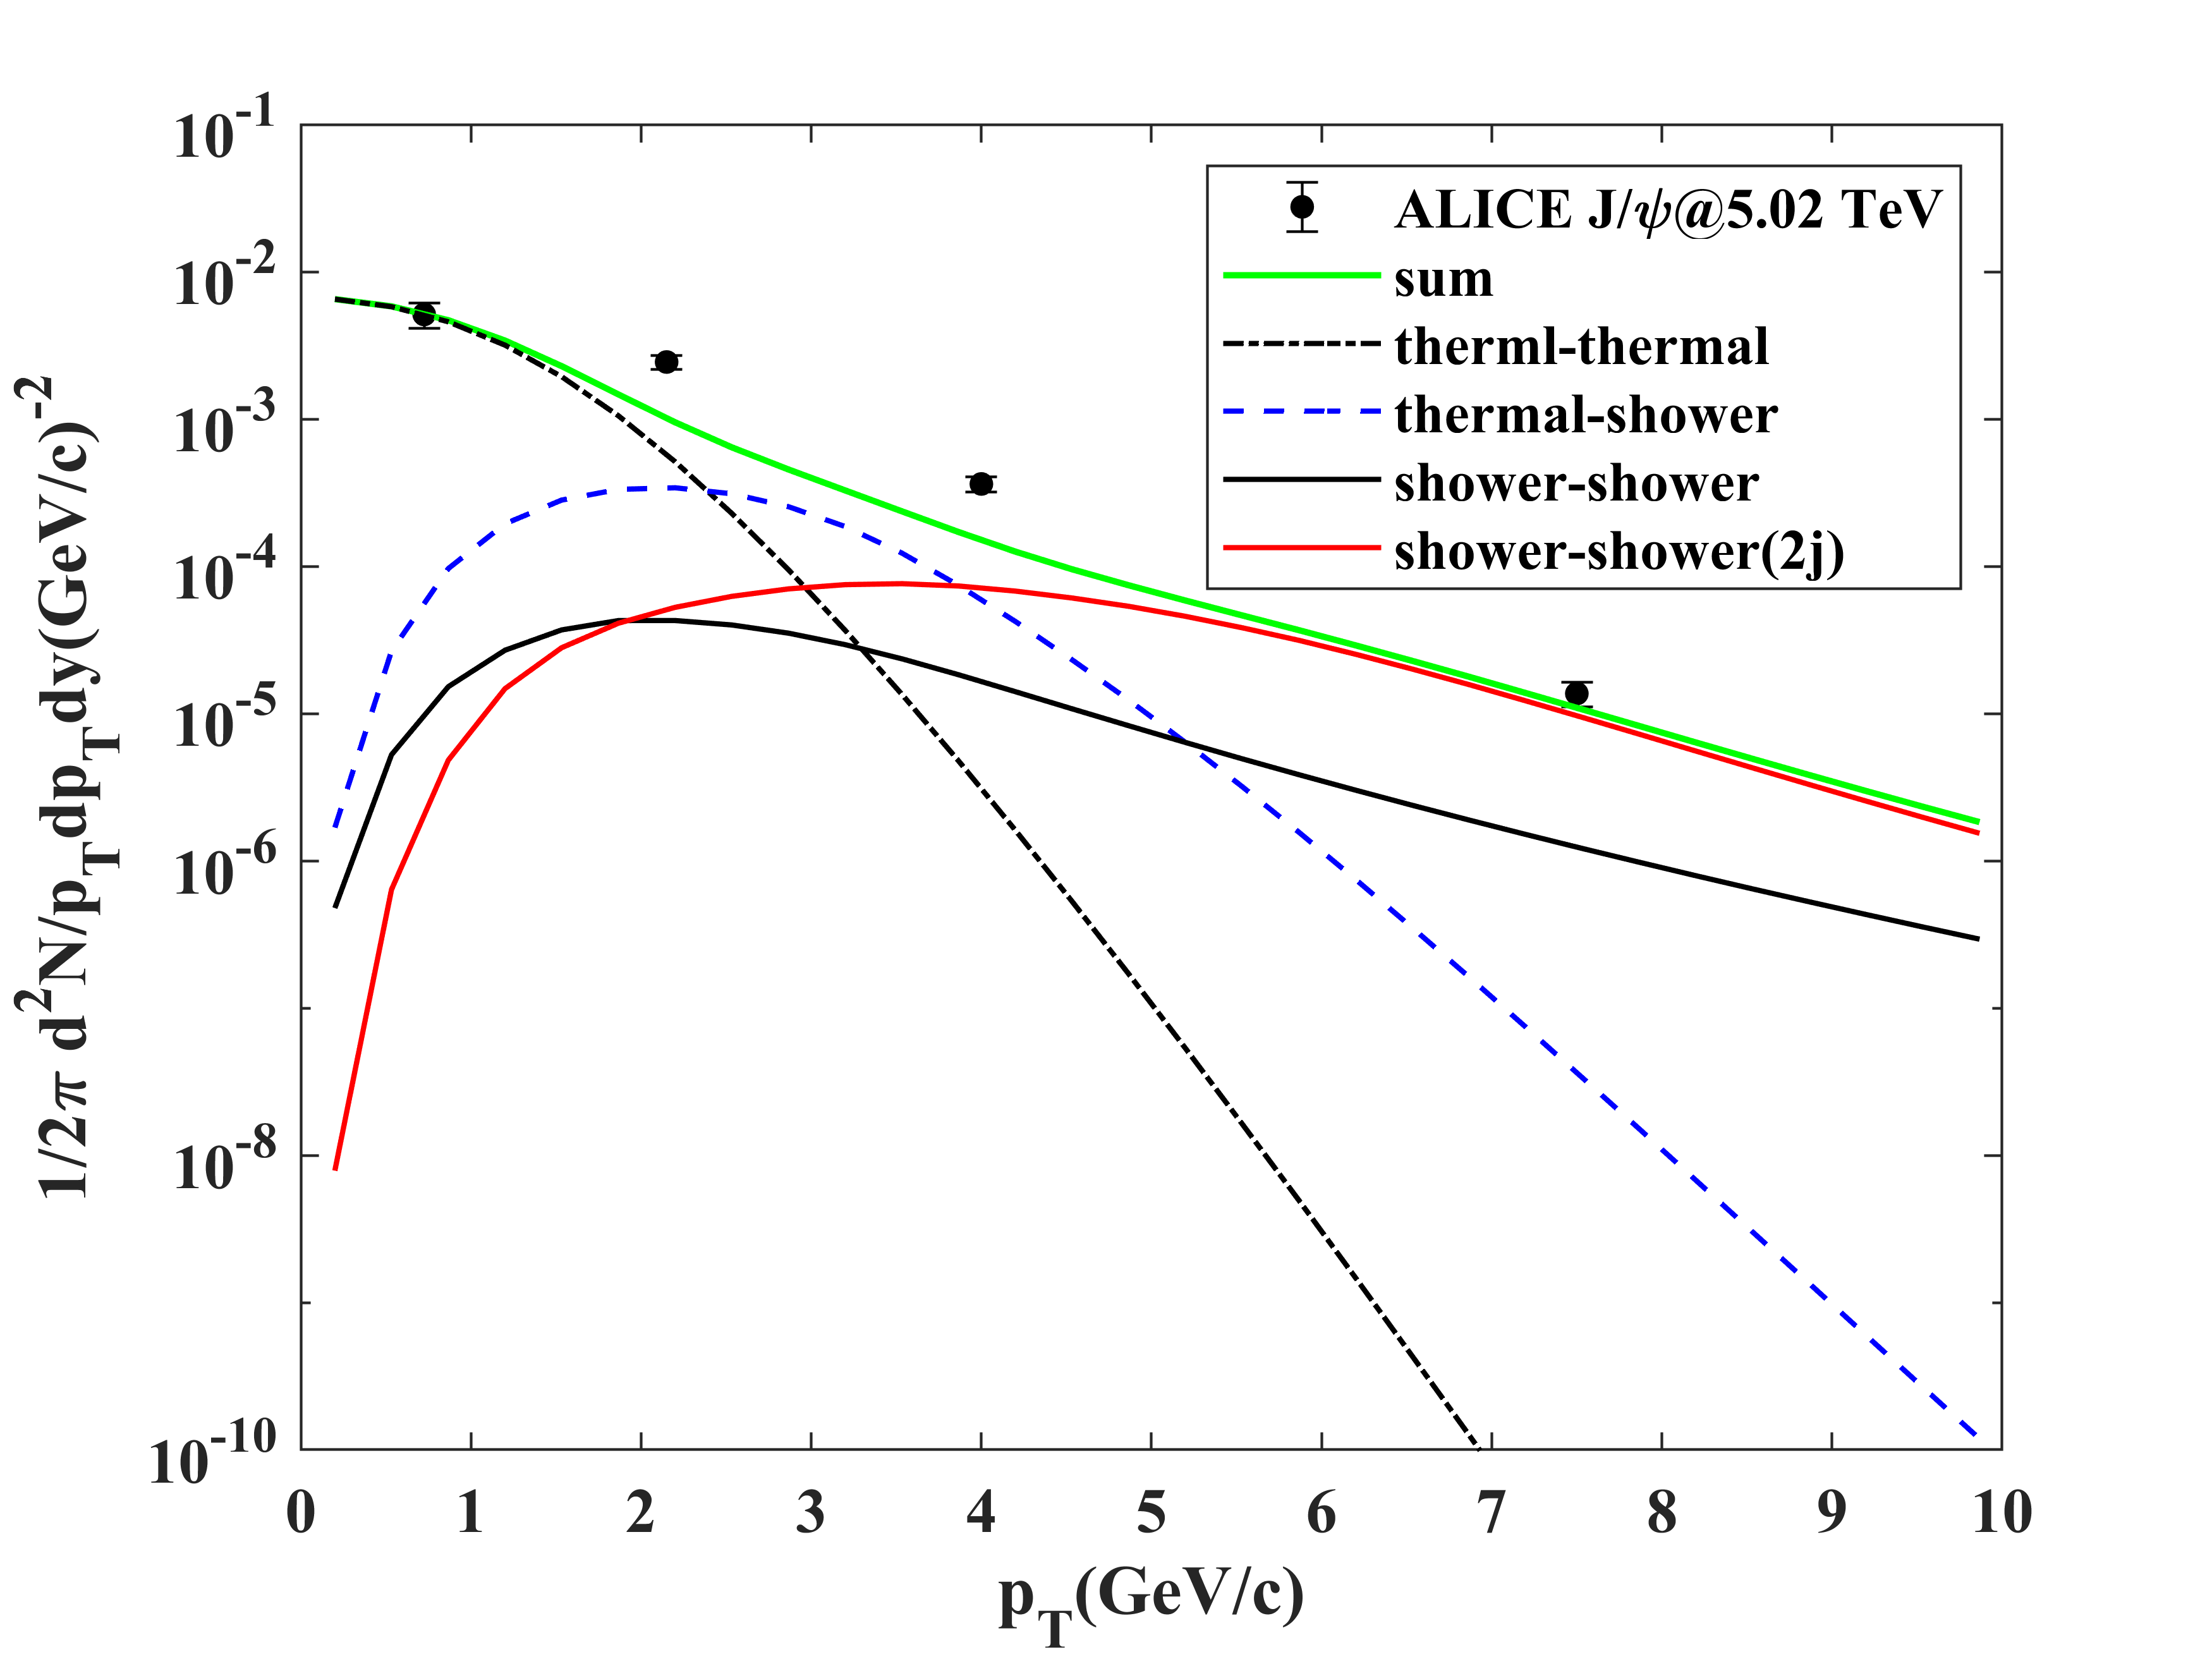
\includegraphics[width=0.45\textwidth]{Jpsi502_230205.png}
	\caption{$J/\psi$ distribution at 5.02 TeV with $\Gamma=10^{-2}$. }
	\label{fig45}
\end{figure}

It is suggested to fix the step size at 0.05 to fit parameters and then turn it down as we need.

\section{MEETING 2023.02.13}
Latest fitted parameters are listed here:
\begin{eqnarray}
	\text{2.76 TeV}&:&  \nonumber \\
	&&T=0.185 \text{ GeV}, \Gamma=10^{-2}, \nonumber \\
	&&\gamma_l=1.0,  \gamma_s=0.8 ,\gamma_c=0.26\nonumber \\
	J/\psi&:& v_T=0.25c,  \\ \nonumber
	&&\beta L\rightarrow \text{0 for charm, 2.39 for gluon}\nonumber\\
	D^0&:& v_T=0.43c,  \beta L=\text{8.0 for all}\nonumber\\
	D_s&:& v_T=0.3c,    \beta L=\text{2.39 for all}.\nonumber\\
	\text{5.02 TeV}&:&  \nonumber \\
	&&\Gamma=10^{-2}, \nonumber \\
	&&\gamma_l=1.0,  \gamma_s=0.8 ,\gamma_c=0.39\nonumber \\
	J/\psi&:& v_T=0.25c,  T=0.190 \text{ GeV},\\ \nonumber
	&&\beta L\rightarrow \text{0 for charm, 0.1 for gluon}\nonumber\\
	D^0&:& v_T=0.5c,  T=0.175 \text{ GeV},\\ \nonumber
	&&\beta L=\text{3.0 for charm, 7.0 for gluon}\nonumber\\
	D_s&:& v_T=0.3c,   T=0.175 \text{ GeV},\\ \nonumber
	&&\beta L=\text{2.0 for charm, 6.0 for gluon}.\nonumber
\end{eqnarray}
Through those above, the spectra are shown below. We have improved the spectra of $D^0$ at 2.76 TeV. Note that $TS$ component in Fig.\ref{fig47} should have been larger than what we see, because $TS$ component is calculated by using step 0.05 for triple integral.
\begin{figure}[H]
	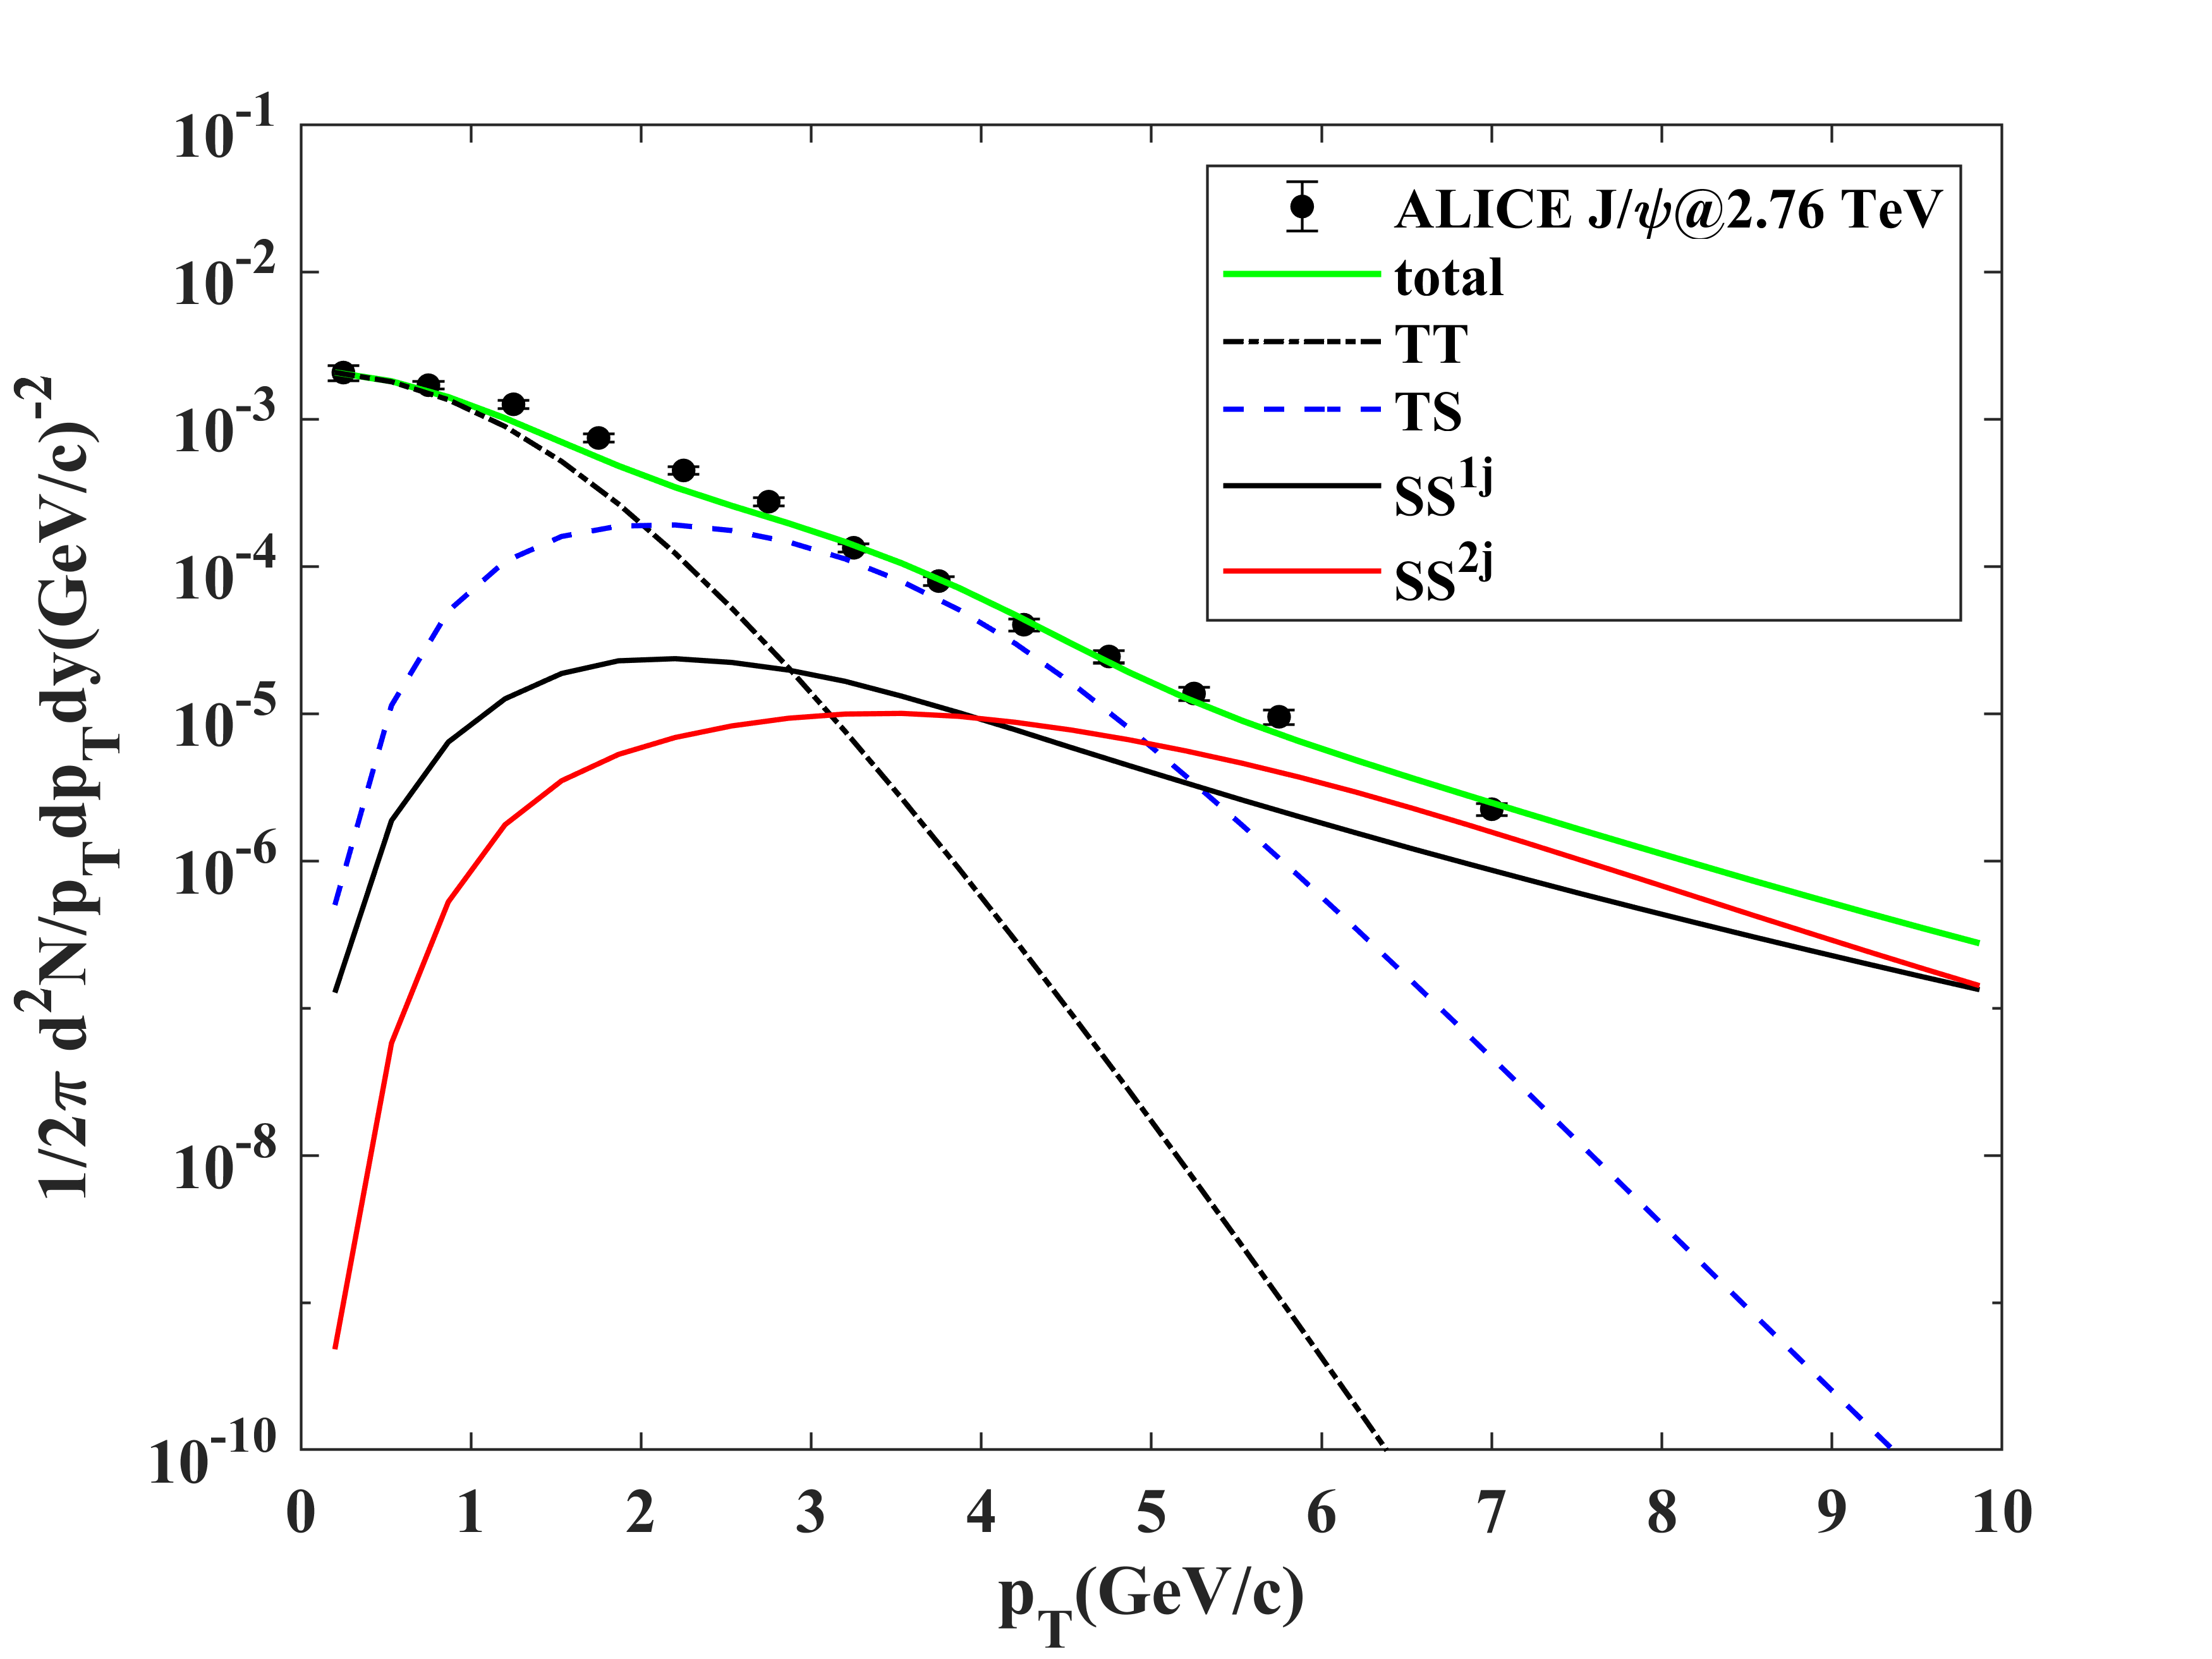
\includegraphics[width=0.45\textwidth]{Jpsi276_230205.png}
	\caption{$J/\psi$ distribution at 2.76 TeV with $\Gamma=10^{-2}$. }
	\label{fig46}
\end{figure}
\begin{figure}[H]
	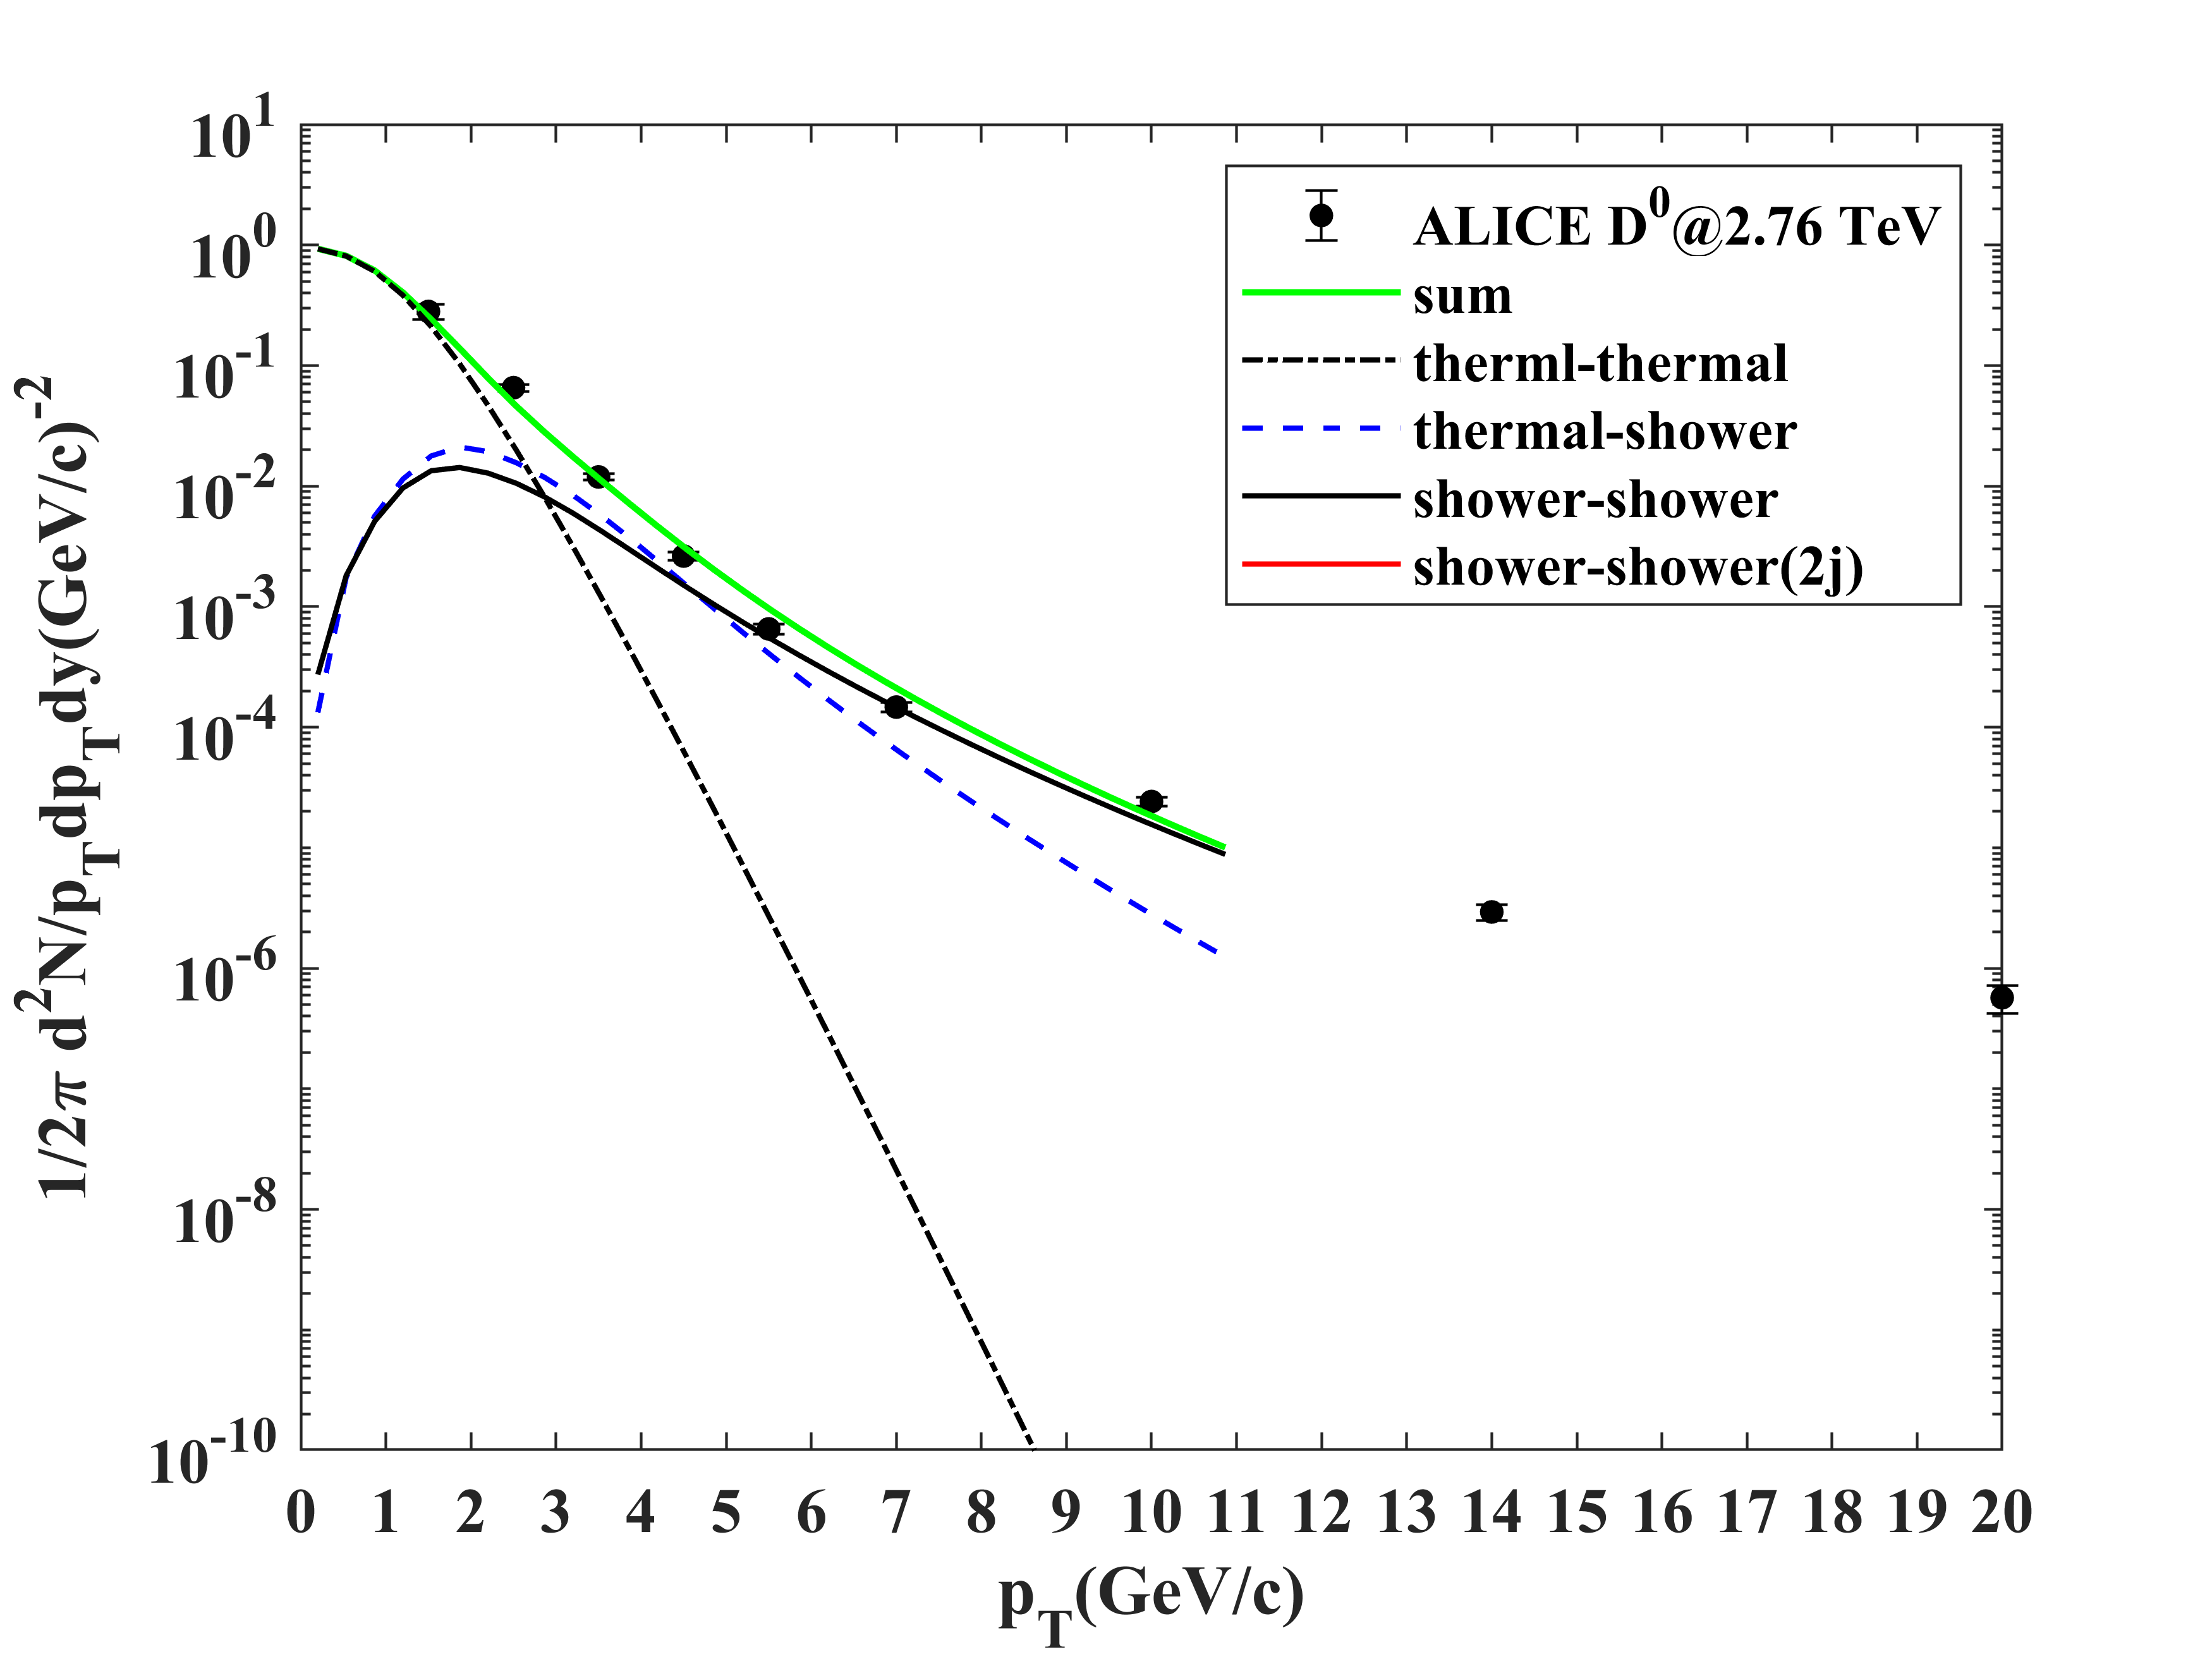
\includegraphics[width=0.45\textwidth]{D0276_230213.png}
	\caption{$D^0$ distribution at 2.76 TeV with $\Gamma=10^{-2}$. }
	\label{fig47}
\end{figure}
\begin{figure}[H]
	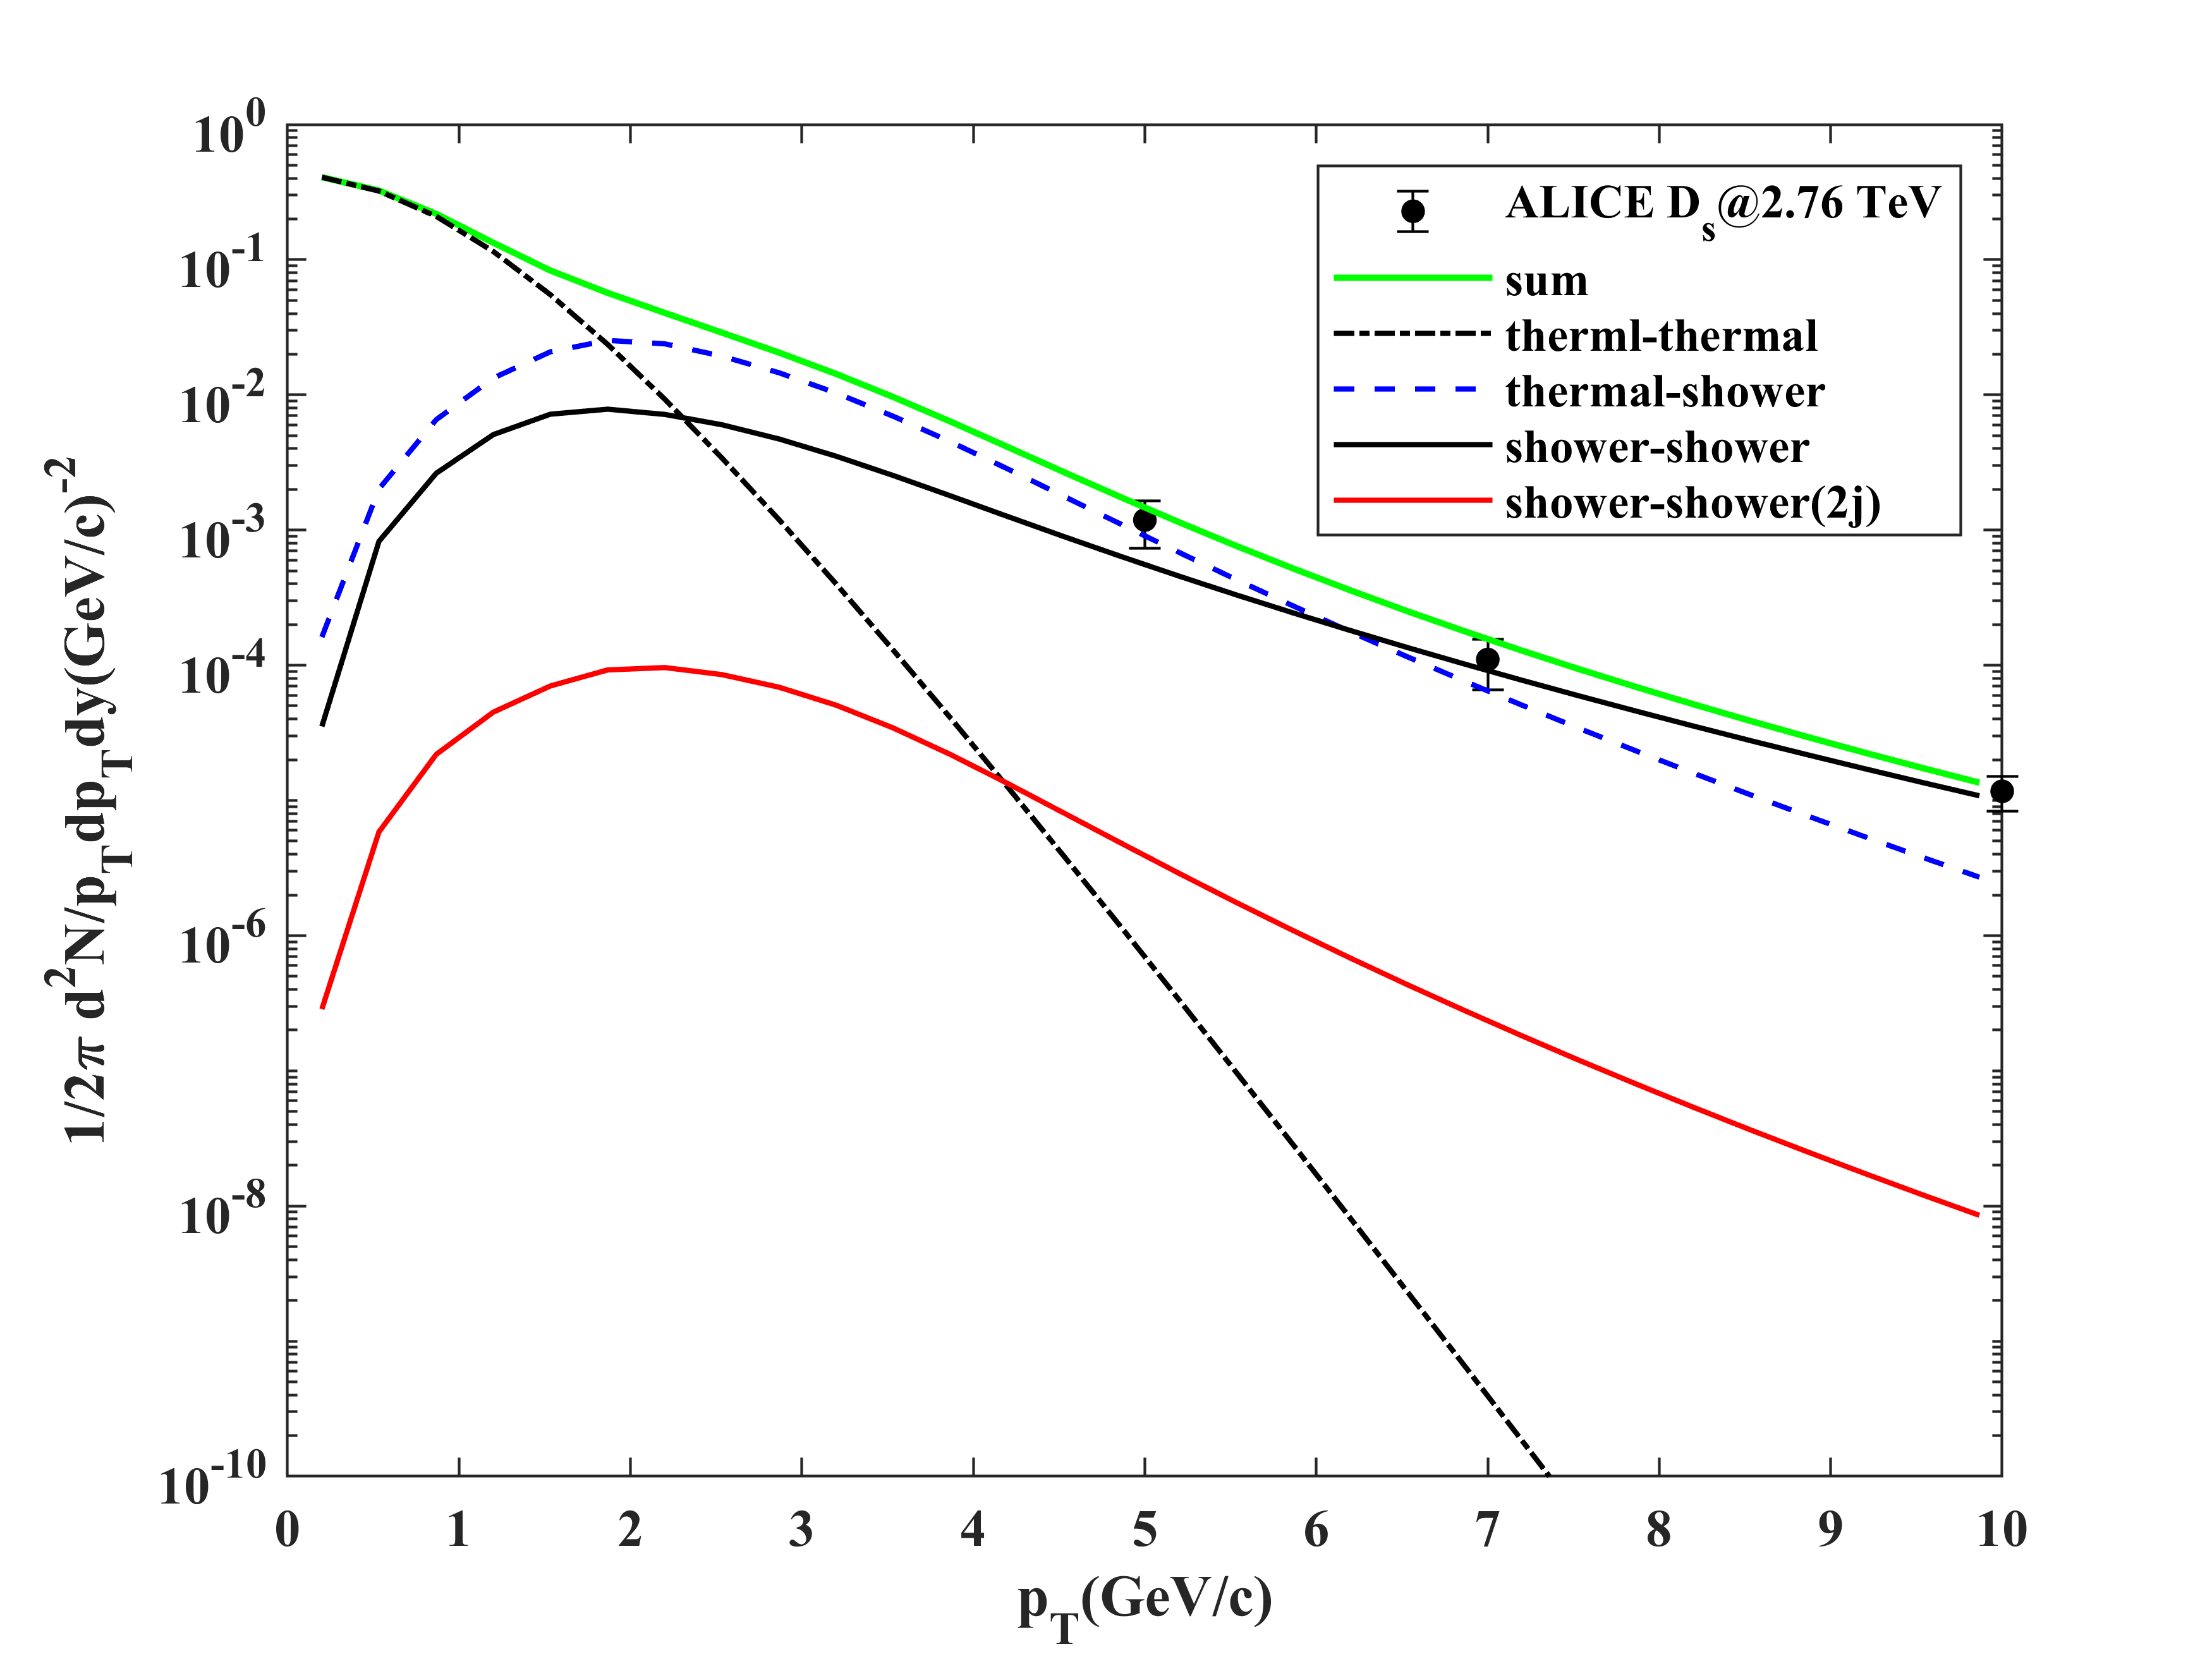
\includegraphics[width=0.45\textwidth]{Ds276_230205.png}
	\caption{$D_s$ distribution at 2.76 TeV with $\Gamma=10^{-2}$. }
	\label{fig48}
\end{figure}
\begin{figure}[H]
	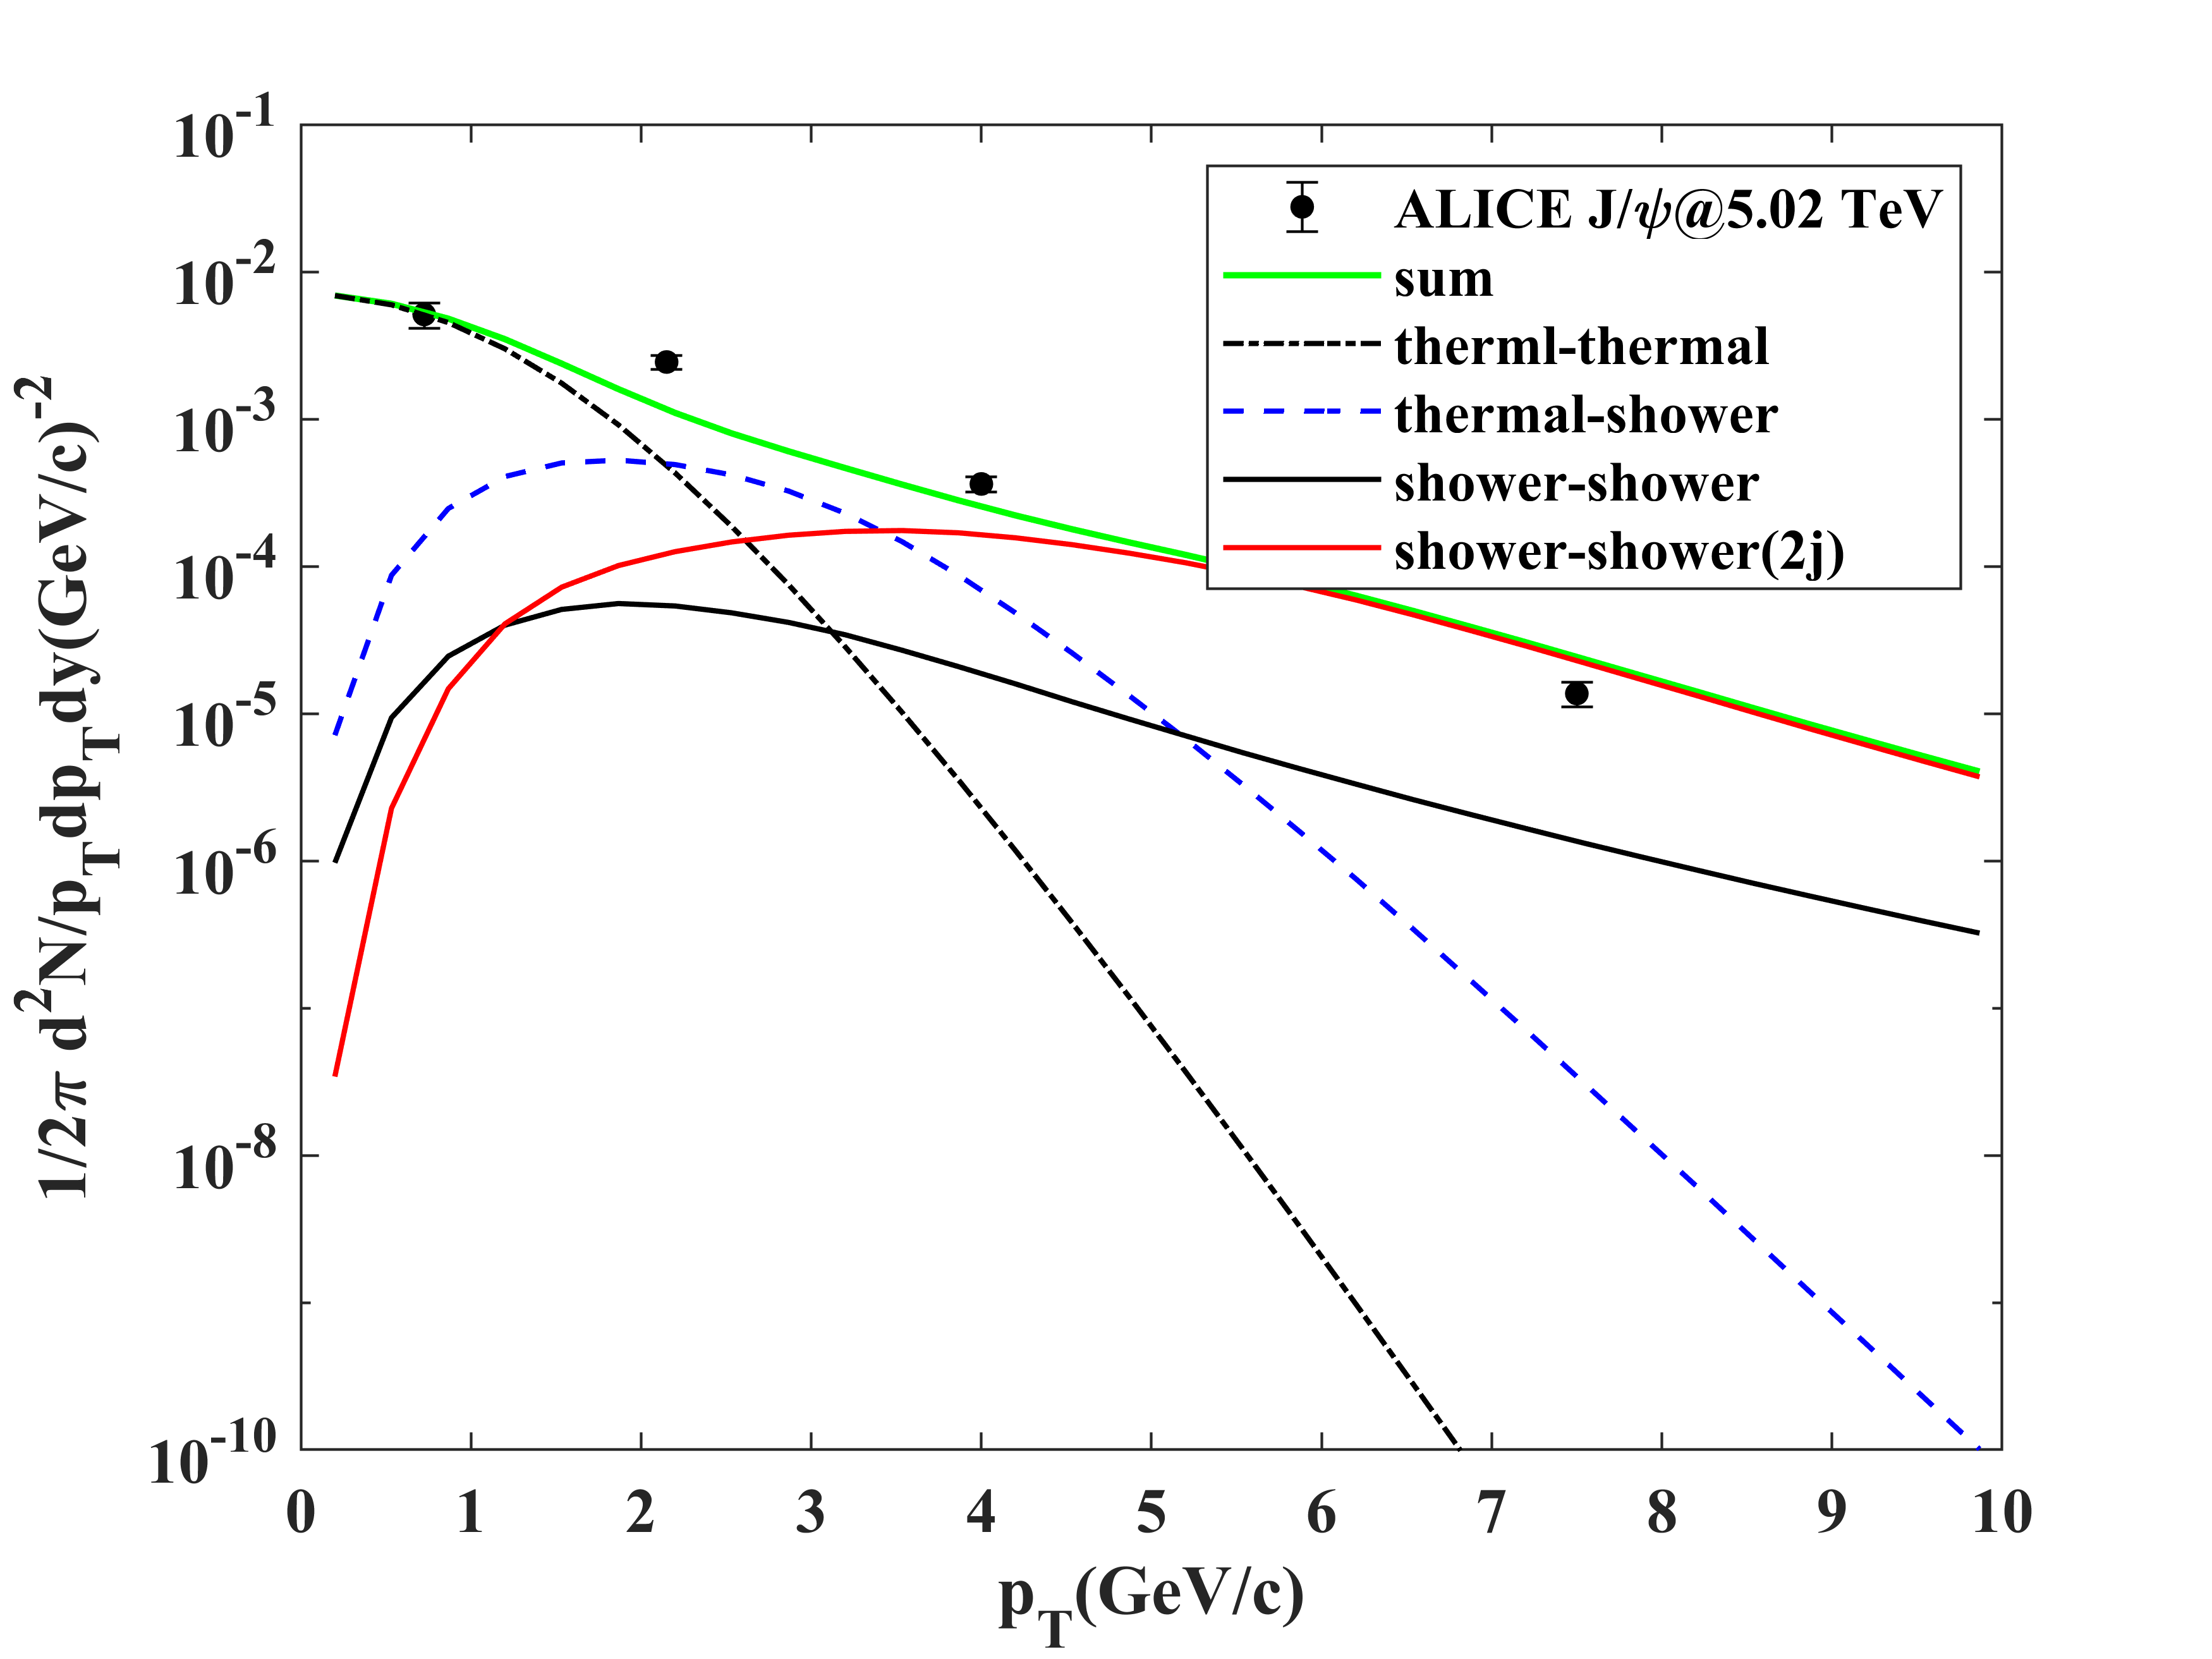
\includegraphics[width=0.45\textwidth]{Jpsi502_230213.png}
	\caption{$J/\psi$ distribution at 5.02 TeV with $\Gamma=10^{-2}$. }
	\label{fig49}
\end{figure}
\begin{figure}[H]
	\includegraphics[width=0.45\textwidth]{D0502_230213.png}
	\caption{$D^0$ distribution at 5.02 TeV with $\Gamma=10^{-2}$. }
	\label{fig50}
\end{figure}
\begin{figure}[H]
	\includegraphics[width=0.45\textwidth]{Ds502_230213.png}
	\caption{$D_s$ distribution at 5.02 TeV with $\Gamma=10^{-2}$. }
	\label{fig51}
\end{figure}

\section{MEETING 2023.02.20}
Since last week, we decline the number of calculated points and fix the first point at $p_T=0.5$ GeV/c owing to uncertain validity for RM at such a low transverse momentum. And before, it is checked that the accuracy of single exponential integral algorithm is suitable(4 significant figures) for our calculation, when the step fdel=0.05. However, for triple exponential integral algorithm, it can be obtained only one significant figure when the step fdel=0.02 and two significant figures when the step fdel=0.01. To derive accurate results with lower computational cost, we choose the step fdel=0.02 finally. Note that the abnormal phenomenon only appeared in the spectra of $D^0$, that the contribution from $SS(1)$ exceeds that from $TS$ at the first point, has vanished after changing the first point and improving accuracy.

Latest fitted parameters and spectra are listed here:
\begin{eqnarray}
	\text{2.76 TeV}&:&  \nonumber \\
	&&T=0.185 \text{ GeV}, \Gamma=10^{-2}, \nonumber \\
	&&\gamma_l=1.0,  \gamma_s=0.8 ,\gamma_c=0.26\nonumber \\
	J/\psi&:& v_T=0.25c,  \\ \nonumber
	&&\beta L\rightarrow \text{0 for charm, 2.39 for gluon}\nonumber\\
	D^0&:& v_T=0.43c,  \beta L=\text{8.0 for all}\nonumber\\
	D_s&:& v_T=0.3c,    \beta L=\text{2.39 for all}.\nonumber\\
	\text{5.02 TeV}&:&  \nonumber \\
	&&\Gamma=10^{-2}, \nonumber \\
	&&\gamma_l=1.0,  \gamma_s=0.8 ,\gamma_c=0.39\nonumber \\
	J/\psi&:& v_T=0.25c,  T=0.190 \text{ GeV},\\ \nonumber
	&&\beta L\rightarrow \text{0 for charm, 0.1 for gluon}\nonumber\\
	D^0&:& v_T=0.5c,  T=0.175 \text{ GeV},\\ \nonumber
	&&\beta L=\text{8.0 for charm and gluon, 5.0 for $\overline{u}$}\nonumber\\
	D_s&:& v_T=0.3c,   T=0.175 \text{ GeV},\\ \nonumber
	&&\beta L=\text{7.0 for charm and gluon, 5.0 for $\overline{s}$}.\nonumber
\end{eqnarray}
\begin{figure}[H]
	\includegraphics[width=0.45\textwidth]{Jpsi276_230205.png}
	\caption{$J/\psi$ distribution at 2.76 TeV with $\Gamma=10^{-2}$. }
	\label{fig52}
\end{figure}
\begin{figure}[H]
	\includegraphics[width=0.45\textwidth]{D0276_230220.png}
	\caption{$D^0$ distribution at 2.76 TeV with $\Gamma=10^{-2}$. }
	\label{fig53}
\end{figure}
\begin{figure}[H]
	\includegraphics[width=0.45\textwidth]{Ds276_230205.png}
	\caption{$D_s$ distribution at 2.76 TeV with $\Gamma=10^{-2}$. }
	\label{fig54}
\end{figure}
\begin{figure}[H]
	\includegraphics[width=0.45\textwidth]{Jpsi502_230213.png}
	\caption{$J/\psi$ distribution at 5.02 TeV with $\Gamma=10^{-2}$. }
	\label{fig55}
\end{figure}
\begin{figure}[H]
	\includegraphics[width=0.45\textwidth]{D0502_230220.png}
	\caption{$D^0$ distribution at 5.02 TeV with $\Gamma=10^{-2}$. }
	\label{fig56}
\end{figure}
\begin{figure}[H]
	\includegraphics[width=0.45\textwidth]{Ds502_230220.png}
	\caption{$D_s$ distribution at 5.02 TeV with $\Gamma=10^{-2}$. }
	\label{fig57}
\end{figure}

\section{MEETING 2023.02.27}
Latest fitted parameters and spectra are listed here:
\begin{eqnarray}
	\text{2.76 TeV}&:&  \nonumber \\
	&&T=0.185 \text{ GeV}, \Gamma=10^{-2}, \nonumber \\
	&&\gamma_l=1.0,  \gamma_s=0.8 ,\gamma_c=0.26\nonumber \\
	J/\psi&:& v_T=0.25c,  \\ \nonumber
	&&\beta L\rightarrow \text{0 for charm, 2.39 for gluon}\nonumber\\
	D^0&:& v_T=0.43c,  \beta L=\text{17.0 for all}\nonumber\\
	D_s&:& v_T=0.3c,    \beta L=\text{2.9 for all}.\nonumber\\
	\text{5.02 TeV}&:&  \nonumber \\
	&&\Gamma=10^{-2}, \nonumber \\
	&&\gamma_l=1.0,  \gamma_s=0.8 ,\gamma_c=0.39\nonumber \\
	J/\psi&:& v_T=0.25c,  T=0.190 \text{ GeV},\\ \nonumber
	&&\beta L\rightarrow \text{0 for charm, 0.1 for gluon}\nonumber\\
	D^0&:& v_T=0.5c,  T=0.175 \text{ GeV},\\ \nonumber
	&&\beta L=\text{17.0 for all}\nonumber\\
	D_s&:& v_T=0.3c,   T=0.175 \text{ GeV},\\ \nonumber
	&&\beta L=\text{7.0 for charm and gluon, 5.0 for $\overline{s}$}.\nonumber
\end{eqnarray}
\begin{figure}[H]
	\includegraphics[width=0.45\textwidth]{Jpsi276_230223.png}
	\caption{$J/\psi$ distribution at 2.76 TeV with $\Gamma=10^{-2}$. }
	\label{fig58}
\end{figure}
\begin{figure}[H]
	\includegraphics[width=0.45\textwidth]{D0276_230223.png}
	\caption{$D^0$ distribution at 2.76 TeV with $\Gamma=10^{-2}$. }
	\label{fig59}
\end{figure}
\begin{figure}[H]
	\includegraphics[width=0.45\textwidth]{Ds276_230223.png}
	\caption{$D_s$ distribution at 2.76 TeV with $\Gamma=10^{-2}$. }
	\label{fig60}
\end{figure}
\begin{figure}[H]
	\includegraphics[width=0.45\textwidth]{Jpsi502_230223.png}
	\caption{$J/\psi$ distribution at 5.02 TeV with $\Gamma=10^{-2}$. }
	\label{fig61}
\end{figure}
\begin{figure}[H]
	\includegraphics[width=0.45\textwidth]{D0502_230223.png}
	\caption{$D^0$ distribution at 5.02 TeV with $\Gamma=10^{-2}$. }
	\label{fig62}
\end{figure}
\begin{figure}[H]
	\includegraphics[width=0.45\textwidth]{Ds502_230223.png}
	\caption{$D_s$ distribution at 5.02 TeV with $\Gamma=10^{-2}$. }
	\label{fig63}
\end{figure}

Considering the unreliable fitted formula Eq.\ref{fit_276} and Eq.\ref{fit_502} in Fig.\ref{fig34} at large momentum, leading to generally inaccurate results at high $p_T$ in spectra above, we direct produce 3000 points from FONLL shown in Fig.\ref{fig64} and read them in program, like the way of MatFiqc.
\begin{figure}[H]
	\includegraphics[width=0.45\textwidth]{charmJet.png}
	\caption{Charm jet distribution $f_c(k)$ produced by FONLL. }
	\label{fig64}
\end{figure}

\section{Meeting 2023.03.05}
In spite of agreement with experimental data, the fitted parameters  seem unreasonable. Thus we will do some check in the followings.

First, all data are plotted in one figure below.
\begin{figure}[H]
	\includegraphics[width=0.45\textwidth]{all_data.png}
	\caption{Experimental data of three mesons at two energy. }
	\label{fig65}
\end{figure}
Second, we check the spectrum of $D^0$, replacing $F'_i(q)$ by $f_i(k)$. In practice, we just set $bL$=0.01, assuming the dynamic length tends to 0, i.e. no momentum decay at creation.
\begin{figure}[H]
	\includegraphics[width=0.45\textwidth]{change_F1iq_to_fik.png}
	\caption{$D^0$ distribution at 2.76 TeV with $\Gamma=10^{-2}$ when $bL$=0.01. }
	\label{fig66}
\end{figure}
Third, the thermal distribution at 2.76 and 5.02 TeV are fitted by $C*exp(-p_T/T)$ respectively.
\begin{figure}[H]
	\includegraphics[width=0.45\textwidth]{Thermal276.png}
	\caption{Thermal parton distribution at 2.76 TeV. }
	\label{fig67}
\end{figure}
\begin{figure}[H]
	\includegraphics[width=0.45\textwidth]{Thermal502.png}
	\caption{Thermal parton distribution at 5.02 TeV. }
	\label{fig68}
\end{figure}
Fourth, we reproduce the results at the beginning of this paper after debugging.
\begin{figure}[H]
	\includegraphics[width=0.45\textwidth]{Jpsi200.png}
	\caption{$J/\psi$ distribution at 200 GeV with $\Gamma=10^{-2}$. }
	\label{fig69}
\end{figure}
\begin{figure}[H]
	\includegraphics[width=0.45\textwidth]{D0200.png}
	\caption{$D^0$ distribution at 200 GeV with $\Gamma=10^{-2}$. }
	\label{fig70}
\end{figure}
\begin{figure}[H]
	\includegraphics[width=0.45\textwidth]{Ds200.png}
	\caption{$D_s$ distribution at 200 GeV with $\Gamma=10^{-2}$. }
	\label{fig71}
\end{figure}


\section{MEETING 2023.03.13}
Last week, we figured out the importance of cutoff in shower, the same as v15(2$\sim$30). Then it is corrected to 3$\sim$30, shown better agreement below.
\begin{figure}[H]
	\includegraphics[width=0.45\textwidth]{Jpsi200_230313.png}
	\caption{$J/\psi$ distribution at 200 GeV with $\Gamma=10^{-2}, q=3\sim30$. }
	\label{fig72}
\end{figure}
\begin{figure}[H]
	\includegraphics[width=0.45\textwidth]{D0200_230313.png}
	\caption{$D^0$ distribution at 200 GeV with $\Gamma=10^{-2}, q=3\sim30$. }
	\label{fig73}
\end{figure}
\begin{figure}[H]
	\includegraphics[width=0.45\textwidth]{Ds200_230313.png}
	\caption{$D_s$ distribution at 200 GeV with $\Gamma=10^{-2}, q=3\sim30$. }
	\label{fig74}
\end{figure}

Thus, we attempt to utilize it to correct the strangeness of parameters for $D^0$. Through a lot of tests below, it seems hard to correct $bL$ from 17.0 to 2.9. In Fig.\ref{fig80}, $bL=15.0$ and $q=3\sim30$ was used and a little improvement was seen.
\begin{figure}[H]
	\includegraphics[width=0.45\textwidth]{D0276_q330.png}
	\caption{$D^0$ distribution at 2.76 TeV with $\Gamma=10^{-2}, q=3\sim30, bL=2.9$. }
	\label{fig75}
\end{figure}
\begin{figure}[H]
	\includegraphics[width=0.45\textwidth]{D0276_q430.png}
	\caption{$D^0$ distribution at 2.76 TeV with $\Gamma=10^{-2}, q=4\sim30, bL=2.9$. }
	\label{fig76}
\end{figure}
\begin{figure}[H]
	\includegraphics[width=0.45\textwidth]{D0276_q830.png}
	\caption{$D^0$ distribution at 2.76 TeV with $\Gamma=10^{-2}, q=8\sim30, bL=2.9$. }
	\label{fig77}
\end{figure}
 \begin{figure}[H]
 	\includegraphics[width=0.45\textwidth]{D0276_q320.png}
 	\caption{$D^0$ distribution at 2.76 TeV with $\Gamma=10^{-2}, q=3\sim20, bL=2.9$. }
 	\label{fig78}
 \end{figure}
 \begin{figure}[H]
	\includegraphics[width=0.45\textwidth]{D0276_q340.png}
	\caption{$D^0$ distribution at 2.76 TeV with $\Gamma=10^{-2}, q=3\sim40, bL=2.9$. }
	\label{fig79}
\end{figure}

 \begin{figure}[H]
	\includegraphics[width=0.45\textwidth]{D0276_q330_bL15.png}
	\caption{$D^0$ distribution at 2.76 TeV with $\Gamma=10^{-2}, q=3\sim30, bL=15$. }
	\label{fig80}
\end{figure}

\section{MEETING 2023.04.10}
Parameters should be modified in v16:
\begin{eqnarray}
	T_c, C_c, \gamma_0, q_0,  gbst
\end{eqnarray}
Question: am, bm in subroutine $meson\_coe$, function FF(IDH, IDparticle, x)


\section{MEETING 2023.05.29}
Since parameters of previous program are unreasonable, we move to v16 constructed from v15. We find that recombination function in \cite{Zhu_2020}(JPG) is different from \cite{Peng2010,Peng2011,Peng:2011zzd}(R. P.), which mainly reflected in whether it includes the parameter $g_M$. We will use the former in v16, including $g_M$. And then the formulae of mesons are given here,
\begin{widetext}
	\begin{eqnarray}
		\frac{dN^{TT}_{D^0}}{d^2p}&=&{5g_{D^0} C_q C_c\over p_0 p_T^6}\int_0^{p_T}dp_1 p_1 e^{-p_1/T_q} (p_T -p_1) e^{-(p_T -p_1)/T_c} (p_T -p_1)^4, \\
		\frac{dN^{TS}_{D^0}}{d^2p}&=&{5g_{D^0} \over p_0 p_T^6}\int_0^{p_T}dp_1 
		p_1(p_T -p_1)^4 [C_q e^{-p_1/T_q} S^c(p_T-p_1)+C_c({p_T\over p_1} -1) e^{-(p_T -p_1)/T_c}S^{\bar{u}}(p_1)] , \\
		\frac{dN^{TT}_{D_s}}{d^2p}&=&{660g_{D_s} C_s C_c\over p_0 p_T^{13}}\int_0^{p_T}dp_1 p_1 e^{-p_1/T_s} (p_T -p_1) e^{-(p_T -p_1)/T_c} p_1^2 (p_T -p_1)^9, \\
		\frac{dN^{TS}_{D_s}}{d^2p}&=&{660g_{D_s} \over p_0 p_T^{13}}\int_0^{p_T}dp_1 
		p_1^3(p_T -p_1)^9 [C_s e^{-p_1/T_s} S^c(p_T-p_1)+C_c({p_T\over p_1} -1) e^{-(p_T -p_1)/T_c}S^{\bar{s}}(p_1)] .
	\end{eqnarray}
\end{widetext}

After fitting, parameters in \ref{parameters} and results are listed here.

\begin{table*}[htbp]
	\centering
	\caption{Parameters used in v16, in which $\gamma_0$ and $q_0$ are only for charm quark.}
	\label{parameters}
	\setlength{\tabcolsep}{4.5mm}{
	\begin{tabular}{|c|ccccccccccc|}
		\hline
		 &$C_q$ & $T_q$ & $C_s$ & $T_s$ & $C_c$ & $T_c$ & $\gamma_0$ & $q_0$ & $g_{J/\psi}$ &  $g_{D^0}$ &  $g_{D_s}$ \\
		\hline
		2.76 TeV &23.2 & 0.39 & 11.0 & 0.51 & 1.8 &0.65 & 1.7 & 10.8 & \multirow{2}{*}{0.04} & \multirow{2}{*}{1}  & \multirow{2}{*}{0.5}  \\ 

		5.02 TeV &22.0 & 0.42 & 10.0 & 0.545 & 2.5 &0.70 & 2.0 & 10.8 &&  & \\
		\hline
	\end{tabular}}
\end{table*}


 \begin{figure}[H]
	\includegraphics[width=0.45\textwidth]{v16_Jpsi_276.png}
	\caption{$J/\psi$ distribution at 2.76 TeV. }
	\label{fig81}
\end{figure}
\begin{figure}[H]
	\includegraphics[width=0.45\textwidth]{v16_D0_276.png}
	\caption{$D^0$ distribution at 2.76 TeV. }
	\label{fig82}
\end{figure}

\begin{figure}[H]
	\includegraphics[width=0.45\textwidth]{v16_Ds_276.png}
	\caption{$D_s$ distribution at 2.76 TeV. }
	\label{fig83}
\end{figure}
 \begin{figure}[H]
	\includegraphics[width=0.45\textwidth]{v16_Jpsi_502.png}
	\caption{$J/\psi$ distribution at 5.02 TeV. }
	\label{fig84}
\end{figure}
\begin{figure}[H]
	\includegraphics[width=0.45\textwidth]{v16_D0_502.png}
	\caption{$D^0$ distribution at 5.02 TeV. }
	\label{fig85}
\end{figure}

\begin{figure}[H]
	\includegraphics[width=0.45\textwidth]{v16_Ds_502.png}
	\caption{$D_s$ distribution at 5.02 TeV. }
	\label{fig86}
\end{figure}
It seems the agreement for $J/\psi$ at 5.02 TeV is not good. However, the better parameters $C_c=2.1, T_c=0.9$ for $J/\psi$ are not suitable for the other two mesons, showed below.
 \begin{figure}[H]
	\includegraphics[width=0.45\textwidth]{v16_Jpsi_502_try.png}
	\caption{$J/\psi$ distribution at 5.02 TeV with $C_c=2.1, T_c=0.9$. }
	\label{fig87}
\end{figure}
\begin{figure}[H]
	\includegraphics[width=0.45\textwidth]{v16_D0_502_try.png}
	\caption{$D^0$ distribution at 5.02 TeV with $C_c=2.1, T_c=0.9$. }
	\label{fig88}
\end{figure}

\begin{figure}[H]
	\includegraphics[width=0.45\textwidth]{v16_Ds_502_try.png}
	\caption{$D_s$ distribution at 5.02 TeV with $C_c=2.1, T_c=0.9$. }
	\label{fig89}
\end{figure}

\section{MEETING 2023.06.12}
In our fitting strategy, $T_c$ and $C_c$ are first determined by fitting with spectrum of $J/\psi$, where $TT$ dominates in the range of 0 to 7 GeV/c. Then $g_M$ can be determined by fitting the components of $TT$ for various mesons. Eventually, $\gamma_0$ and $q_0$ should be fine-tuned by fitting the components of $TS$ .
\begin{table*}[htbp]
	\centering
	\caption{Parameters used in v16, in which $\gamma_0$ and $q_0$ are only for charm quark.}
	\label{parameters0605}
	\setlength{\tabcolsep}{4.5mm}{
		\begin{tabular}{|c|ccccccccccc|}
			\hline
			&$C_q$ & $T_q$ & $C_s$ & $T_s$ & $C_c$ & $T_c$ & $\gamma_0$ & $q_0$ & $g_{J/\psi}$ &  $g_{D^0}$ &  $g_{D_s}$ \\
			\hline
			2.76 TeV &23.2 & 0.39 & 11.0 & 0.51 & 1.4 &0.7 & 3.0 & 7.0 & \multirow{2}{*}{0.04} & \multirow{2}{*}{0.7}  & \multirow{2}{*}{0.2}  \\ 
			
			5.02 TeV &22.0 & 0.42 & 10.0 & 0.545 & 2.1 &0.9 & 3.0 & 7.0 &&  & \\
			\hline
	\end{tabular}}
\end{table*}

 \begin{figure}[H]
	\includegraphics[width=0.45\textwidth]{v16_Jpsi_276_0612.png}
	\caption{$J/\psi$ distribution at 2.76 TeV. }
	\label{fig90}
\end{figure}
\begin{figure}[H]
	\includegraphics[width=0.45\textwidth]{v16_D0_276_0612.png}
	\caption{$D^0$ distribution at 2.76 TeV. }
	\label{fig91}
\end{figure}

\begin{figure}[H]
	\includegraphics[width=0.45\textwidth]{v16_Ds_276_0612.png}
	\caption{$D_s$ distribution at 2.76 TeV. }
	\label{fig92}
\end{figure}
\begin{figure}[H]
	\includegraphics[width=0.45\textwidth]{v16_Jpsi_502_0612.png}
	\caption{$J/\psi$ distribution at 5.02 TeV. }
	\label{fig93}
\end{figure}
\begin{figure}[H]
	\includegraphics[width=0.45\textwidth]{v16_D0_502_0612.png}
	\caption{$D^0$ distribution at 5.02 TeV. }
	\label{fig94}
\end{figure}

\begin{figure}[H]
	\includegraphics[width=0.45\textwidth]{v16_Ds_502_0612.png}
	\caption{$D_s$ distribution at 5.02 TeV. }
	\label{fig95}
\end{figure}

\section{MEETING 2023.06.19}
Last week, we found the data of $J/\psi$ at 2.76 TeV are not at mid-rapidity, which gives $2.5<y<4.0$. And $R_{AA}$, related with parameter $q_0$, are given in \cite{D0_276,Ds_276,jpsi_502,D0_502,Ds_502}. After scanning, latest parameters are given below.
\begin{table*}[htbp]
	\centering
	\caption{Parameters used in v16, in which $\gamma_0$ and $q_0$ are only for charm quark.}
	\label{parameters0619}
	\setlength{\tabcolsep}{4.5mm}{
		\begin{tabular}{|c|ccccccccccc|}
			\hline
			&$C_q$ & $T_q$ & $C_s$ & $T_s$ & $C_c$ & $T_c$ & $\gamma_0$ & $q_0$ & $g_{J/\psi}$ &  $g_{D^0}$ &  $g_{D_s}$ \\
			\hline
			2.76 TeV &23.2 & 0.39 & 11.0 & 0.51 & 2.7 &0.7 & 2.8 & 6.7 & \multirow{2}{*}{0.05} & \multirow{2}{*}{0.7}  & \multirow{2}{*}{0.24}  \\ 
			
			5.02 TeV &22.0 & 0.42 & 10.0 & 0.545 & 2.2 &0.83 & 3.9 & 5.8 &&  & \\
			\hline
	\end{tabular}}
\end{table*}

\begin{figure}[H]
	\includegraphics[width=0.45\textwidth]{Jpsi_276.png}
	\caption{$J/\psi$ distribution at 2.76 TeV. }
	\label{fig96}
\end{figure}
\begin{figure}[H]
	\includegraphics[width=0.45\textwidth]{D0_276.png}
	\caption{$D^0$ distribution at 2.76 TeV. }
	\label{fig97}
\end{figure}

\begin{figure}[H]
	\includegraphics[width=0.45\textwidth]{Ds_276.png}
	\caption{$D_s$ distribution at 2.76 TeV. }
	\label{fig98}
\end{figure}
\begin{figure}[H]
	\includegraphics[width=0.45\textwidth]{Jpsi_502.png}
	\caption{$J/\psi$ distribution at 5.02 TeV. }
	\label{fig99}
\end{figure}
\begin{figure}[H]
	\includegraphics[width=0.45\textwidth]{D0_502.png}
	\caption{$D^0$ distribution at 5.02 TeV. }
	\label{fig100}
\end{figure}

\begin{figure}[H]
	\includegraphics[width=0.45\textwidth]{Ds_502.png}
	\caption{$D_s$ distribution at 5.02 TeV. }
	\label{fig101}
\end{figure}

%\section*{Acknowledgements}
\begin{thebibliography}{99}

\bibitem{fik14}
D.~K. Srivastava, C.~Gale, and R.~J. Fries, ``Large mass dileptons from the
passage of jets through a quark gluon plasma,'' \emph{Physical Review C},
vol.~67, no.~3, mar 2003. [Online]. Available:
\url{https://doi.org/10.1103%2Fphysrevc.67.034903}

\bibitem{fik15}
C.~M. Ko and W.~Liu, ``Suppression of heavy quarks in heavy-ion collisions,''
\emph{Nuclear Physics A}, vol. 783, no.~1, pp. 233--240, 2007, proceedings of
the 2nd International Conference on Hard and Electromagnetic Probes of
High-Energy Nuclear Collisions. [Online]. Available:
\url{https://www.sciencedirect.com/science/article/pii/S0375947406008232}

\bibitem{Zhu_2020}
L.~Zhu and R.~C. Hwa, ``A unified study of the production of all identified
hadrons over wide ranges of transverse momenta at {LHC},'' \emph{Journal of
	Physics G: Nuclear and Particle Physics}, vol.~47, no.~5, p. 055102, mar
2020. [Online]. Available: \url{https://doi.org/10.1088/1361-6471/ab6edf}

\bibitem{jpsi_276}
The ALICE collaboration., Adam, J., Adamová, D. et al. Differential studies of inclusive $J/\Psi$ and $\Psi$(2S) production at forward rapidity in Pb-Pb collisions at $\sqrt{ s_{NN} }$=2.76 TeV. J. High Energ. Phys. 2016, 179 (2016). 
\url{https://doi.org/10.1007/JHEP05(2016)179}

\bibitem{jpsi_502}
\textbf{ALICE} collaborations, S.~Acharya et al, ``Centrality and transverse
momentum dependence of inclusive $J/\Psi$ production at midrapidity in Pb-Pb
collisions at $\sqrt{s_{NN}}$=5.02 TeV,'' \emph{Physics Letters B}, vol. 805, p. 135434,
2020. [Online]. Available:
\url{https://www.sciencedirect.com/science/article/pii/S0370269320302380}

\bibitem{D0_276}
The ALICE collaboration., Adam, J., Adamová, D. et al. Transverse momentum dependence of D-meson production in Pb-Pb collisions at $\sqrt{s_{NN}}$=2.76 TeV. J. High Energ. Phys. 2016, 81 (2016). \url{https://doi.org/10.1007/JHEP03(2016)081}

\bibitem{D0_502}
The ALICE collaboration., Acharya, S., Adamová, D. et al. Prompt $D^0$, $D^+$, and $D^{*+}$ production in Pb–Pb collisions at $\sqrt{s_{NN}}$ = 5.02 TeV. J. High Energ. Phys. 2022, 174 (2022). \url{https://doi.org/10.1007/JHEP01(2022)174}

\bibitem{Ds_276}
The ALICE collaboration., Adam, J., Adamová, D. et al. Measurement of $D^+_s$
production and nuclear modification factor in Pb-Pb collisions at $\sqrt{s_{NN}}$=2.76 TeV. J. High Energ. Phys. 2016, 82 (2016). 
\url{https://doi.org/10.1007/JHEP03(2016)082}

\bibitem{Ds_502}
\textbf{ALICE} collaborations, S.~Acharya et al, ``Measurement of prompt $D_s^+$-meson
production and azimuthal anisotropy in Pb-Pb collisions at $\sqrt{s_{NN}}$=5.02 TeV,''
\emph{Physics Letters B}, vol. 827, p. 136986, 2022. [Online]. Available:
\url{https://www.sciencedirect.com/science/article/pii/S0370269322001204}

\bibitem{Liu:2008bw}
W.~Liu and R.~J.~Fries,
%``Heavy Quark Production from Jet Conversions in a Quark-Gluon Plasma,''
Phys. Rev. C \textbf{78}, 037902 (2008)
doi:10.1103/PhysRevC.78.037902
[arXiv:0805.1093 [nucl-th]].
%17 citations counted in INSPIRE as of 03 Sep 2022

%\cite{Peng:2011zzd}
\bibitem{Peng:2011zzd}
R.~Peng, C.~B.~Yang and C.~B.~Yang,
%``$J/\psi$ production and elliptic flow parameter $v_2$ at LHC energy,''
Phys. Scripta \textbf{84}, 035202 (2011)
doi:10.1088/0031-8949/84/03/035202
[arXiv:1103.3346 [hep-ph]].
%1 citations counted in INSPIRE as of 07 Sep 2022

\bibitem{Zhu_cutoff}
L.~Zhu and R.~Hwa, ``Centrality and transverse momentum dependencies of
minijets and hadrons in au-au collisions,'' \emph{Physical Review C},
vol.~88, 07 2013.

\bibitem{PhysRevC.84.064914}
R.~C. Hwa and L.~Zhu, ``Spectra of identified hadrons in pb-pb collisions at
2.76 tev at the cern large hadron collider,'' \emph{Phys. Rev. C}, vol.~84,
p. 064914, Dec 2011. [Online]. Available:
\url{https://link.aps.org/doi/10.1103/PhysRevC.84.064914}

\bibitem{Peng2011}
R.~Peng and C.~B. Yang, ``Productions of heavy flavored mesons in relativistic heavy ion collisions in the recombination model,'' \emph{International Journal of Modern Physics E}, vol.~20, no.~5, pp. 1213--1226, May 2011. doi: 10.1142/S0218301311018356. url: \url{https://doi.org/10.1142/S0218301311018356}.

\bibitem{Peng2010}
R.~Peng and C.~B. Yang, ``Production of baryon-antibaryon pairs in relativistic heavy ion collisions with the recombination model,'' \emph{Nuclear Physics A}, vol.~837, no.~3-4, pp. 215--224, Nov. 2010. doi: 10.1016/j.nuclphysa.2010.05.057.

\end{thebibliography}

\end{document}




